%% Copyright (C) 2009-2010, Gostai S.A.S.
%%
%% This software is provided "as is" without warranty of any kind,
%% either expressed or implied, including but not limited to the
%% implied warranties of fitness for a particular purpose.
%%
%% See the LICENSE file for more information.

\documentclass[openright,twoside,11pt,final]{book}
  \usepackage{gostai-documentation}
  \usepackage{nameref}

\newcommand{\UBinary}{\lstinline{UBinary}\xspace}
\newcommand{\UImage}{\lstinline{UImage}\xspace}
\newcommand{\UList}{\lstinline{UList}\xspace}
\newcommand{\UObjectHub}{\lstinline{UObjectHub}\xspace}
\newcommand{\UObject}{\lstinline{UObject}\xspace}
\newcommand{\USound}{\lstinline{USound}\xspace}
\newcommand{\UVar}{\lstinline{UVar}\xspace}
\newcommand{\UEvent}{\lstinline{UEvent}\xspace}

\usepackage{config}
\newcommand{\uobjectsDir}{\absTopSrcdir/sdk-remote/src/urbi}

%% -------------- %%
%% Experimental.  %%
%% -------------- %%

\newcommand{\experimentalremoved}
{%
  \begin{quote}%
    This feature is experimental.  It might be changed, or even removed.%
    Feedback on its use would be appreciated.%
  \end{quote}%
}

\newcommand{\experimental}
{%
  \begin{quote}%
    This feature is experimental.  It might be changed in the future.
    Feedback on its use would be appreciated.%
  \end{quote}%
}

\title{The Urbi Software Development Kit}
\subtitle{Version \packageVersion}
\date{\VcsDay\\(Revision \VcsDescription)}
\author{Gostai}

\begin{document}

\maketitle

This documentation is updated regularly on the Gostai Web site both as a
\href{\docurl/urbi-sdk.pdf}{PDF document}, and as a
\href{\docurl/urbi-sdk.htmldir}{set of HTML pages}.  You may also want to
look at the documentation of the latest versions.

\newcommand{\versionItem}[2]
{
\item[\packageName{} #1] #2.

  \begin{itemize}
  \item \url{\downloadUrl/\packageTarname/#1/doc}
  \item \url{\downloadUrl/\packageTarname/#1/doc/urbi-sdk.pdf}
  \item \url{\downloadUrl/\packageTarname/#1/doc/urbi-sdk.htmldir}
  \item \url{\downloadUrl/\packageTarname/#1/doc/sdk-remote.htmldir} \\
    The Doxygen documentation of SDK Remote.
  \end{itemize}
}
\begin{description}
\versionItem{\packageVersion}{This version}
\versionItem{\packageMajor.\packageMinor.x}{The latest version of the
  \packageMajor.\packageMinor{} family of versions}
\versionItem{\packageMajor.x}{The latest version (also available as
  \url{\downloadUrl/\packageTarname/doc})}
\end{description}

%% Copyright (C) 2009-2010, Gostai S.A.S.
%%
%% This software is provided "as is" without warranty of any kind,
%% either expressed or implied, including but not limited to the
%% implied warranties of fitness for a particular purpose.
%%
%% See the LICENSE file for more information.

\chapter{Introduction}

\usdk is a fully-featured environment to orchestrate complex
organizations of components.  It relies on a middleware architecture
that coordinates components named UObjects.  It also features \us, a
scripting language that can be used to write orchestration programs.

\section{\urbi and UObjects}

\urbi makes the orchestration of independent, concurrent, components
easier.  It was first designed for robotics: it provides all the
needed features to coordinate the execution of various components
(actuators, sensors, software devices that provide features such as
text-to-speech, face recognition and so forth).  Languages such as
\Cxx are well suited to program the local, low-level, handling of
these hardware or software devices; indeed one needs efficiency, small
memory footprint, and access to low-level hardware details.  Yet, when
it comes to component orchestration and coordination, in a word, when
it comes to addressing concurrency, it can be tedious to use such
languages.

Middleware infrastructures make possible to use remote components as
if they were local, to allow concurrent execution, to make synchronous
or asynchronous requests and so forth.  The \dfn{UObject} \Cxx
architecture provides exactly this: a common API that allows
conforming components to be used seamlessly in highly concurrent
settings.  Components need not be designed with UObjects in mind,
rather, UObjects are typically ``shells'' around ``regular''
components.

Components with an UObject interface are naturally supported by the
\us programming language.  This provides a tremendous help: one can
interact with these components (making queries, changing them,
observing their state, monitoring various kinds of events and so
forth), which provides a huge speed-up during development.

Finally, note that, although made with robots in mind, the UObject
architecture is well suited to tame any heavily concurrent
environment, such as video games or complex systems in general.

\section{\urbi and \us}

\us is a programming language primarily designed for robotics. It's a
dynamic, prototype-based, object-oriented scripting language. It
supports and emphasizes parallel and event-based programming, which
are very popular paradigms in robotics, by providing core primitives
and language constructs.

Its main features are:
\begin{itemize}
\item syntactically close to \Cxx. If you know \C or \Cxx, you can
  easily write \us programs.
\item fully integrated with \Cxx. You can bind \Cxx classes in \us
  seamlessly. \us is also integrated with many other languages such as
  \java, \matlab or \python.
\item object-oriented. It supports encapsulation, inheritance and
  inclusion polymorphism. Dynamic dispatching is available through
  monomethods --- just as \Cxx, \Cs or \java.
\item concurrent. It provides you with natural constructs to run and
  control high numbers of interacting concurrent tasks.
\item event-based. Triggering events and reacting to them is
  absolutely straightforward.
\item functional programming.  Inspired by languages such as \lisp or
  \caml, \us features first class functions and pattern matching.
\item client/server.  The interpreter accepts multiple connections
  from different sources (human users, robots, other servers \ldots)
  and enables them to interact.
\item distributed.  You can run objects in different processes,
  potentially remote computers across the network.
\end{itemize}

\section{Genesis}

\urbi what first designed and implemented by Jean-Christophe Baillie,
together with Matthieu Nottale.  Because its users wildly acclaimed it,
Jean-Christophe founded Gostai, a France-based Company that develops
software for robotics with a strong emphasis on personal robotics.

\paragraph{Authors}
\usdk 1 was further developed by Akim Demaille, Guillaume Deslandes, Quentin
Hocquet, and Benoît Sigoure.

The \usdk 2 project was started and developed by Akim Demaille, Quentin
Hocquet, Matthieu Nottale, and Benoît Sigoure.  Samuel Tardieu provided an
immense help during the year 2008, in particular for the concurrency and
event support.

The maintenance is currently carried out by Akim Demaille, Quentin
Hocquet, and Matthieu Nottale.  Jean-Christophe Baillie is still
deeply involved in the development of \us, he regularly submits ideas,
and occasionally even code!

\paragraph{Contributors}

A number of people contributed significantly to \urbi, including Romain
Bezut, Thomas Moulard, Nicolas Pierron.

\section{Outline}

This multi-part document provides a complete guide to Urbi.  See
\autoref{sec:notations} for the various notations that are used in the
document.

\newenvironment{partDescription}[2]
{%
  \item[\autoref{#1} --- \nameref{#1}]~\\%
  #2
  \begin{description}%
    \let\itemOrig\item%
    \renewcommand{\item}[1][]{\itemOrig[~~\autoref{##1} --- \nameref{##1}]~\\}%
  }{%
  \end{description}%
}

%%% Keep sync with urbi-sdk.tex.
\begin{description}
%% Copyright (C) 2010, Gostai S.A.S.
%%
%% This software is provided "as is" without warranty of any kind,
%% either expressed or implied, including but not limited to the
%% implied warranties of fitness for a particular purpose.
%%
%% See the LICENSE file for more information.

\begin{partDescription}{part:specs}
  {
    %
    This part defines the specifications of the \us language version
    2.0. It defines the expected behavior from the \us interpreter,
    the standard library, and the \sdk. It can be used to check
    whether some code is valid, or browse \us or \Cxx \api for a
    desired feature. Random reading can also provide you with advanced
    knowledge or subtleties about some \us aspects.

    This part is not an \us tutorial; it is not structured in a
    progressive manner and is too detailed.  Think of it as a
    dictionary: one does not learn a foreign language by reading a
    dictionary. The \us Tutorial (\autoref{part:tut}), or the live \us
    tutorial built in the interpreter are good introductions to \us.

    This part does not aim at giving advanced programming
    techniques. Its only goal is to define the language and its
    libraries.
    %
  }
\item[sec:tools]
  Presentation and usage of the different tools available with the
  \urbi framework related to \us, such as the \urbi server, the
  command line client, \umake, \ldots

\item[sec:lang]
  Core constructs of the language and their behavior.

\item[sec:stdlib]
  Listing of all classes and methods provided in the standard library.

\item[sec:specs:ros] \urbi provides a set of tools to communicate with ROS
  (Robot Operating System). For more information about ROS, see
  \url{http://www.ros.org}.  \urbi, acting as a ROS node, is able to
  interact with the ROS world.

\item[sec:naming]
  Also known as ``The \urbi Naming Standard'': naming conventions in
  for standard hardware/software devices and components implemented as
  UObject and the corresponding slots/events to access them.

%\item[sec:sdk]
%  The \urbi software development kit that enable to
%  interact with \urbi from \Cxx.
\end{partDescription}


%%% Local Variables:
%%% mode: latex
%%% TeX-master: "../urbi-sdk"
%%% ispell-dictionary: "american"
%%% ispell-personal-dictionary: "../urbi.dict"
%%% fill-column: 76
%%% End:

%% Copyright (C) 2010, Gostai S.A.S.
%%
%% This software is provided "as is" without warranty of any kind,
%% either expressed or implied, including but not limited to the
%% implied warranties of fitness for a particular purpose.
%%
%% See the LICENSE file for more information.

\begin{partDescription}{part:specs}
  {
    %
    This part defines the specifications of the \us language version
    2.0. It defines the expected behavior from the \us interpreter,
    the standard library, and the \sdk. It can be used to check
    whether some code is valid, or browse \us or \Cxx \api for a
    desired feature. Random reading can also provide you with advanced
    knowledge or subtleties about some \us aspects.

    This part is not an \us tutorial; it is not structured in a
    progressive manner and is too detailed.  Think of it as a
    dictionary: one does not learn a foreign language by reading a
    dictionary. The \us Tutorial (\autoref{part:tut}), or the live \us
    tutorial built in the interpreter are good introductions to \us.

    This part does not aim at giving advanced programming
    techniques. Its only goal is to define the language and its
    libraries.
    %
  }
\item[sec:tools]
  Presentation and usage of the different tools available with the
  \urbi framework related to \us, such as the \urbi server, the
  command line client, \umake, \ldots

\item[sec:lang]
  Core constructs of the language and their behavior.

\item[sec:stdlib]
  Listing of all classes and methods provided in the standard library.

\item[sec:specs:ros] \urbi provides a set of tools to communicate with ROS
  (Robot Operating System). For more information about ROS, see
  \url{http://www.ros.org}.  \urbi, acting as a ROS node, is able to
  interact with the ROS world.

\item[sec:naming]
  Also known as ``The \urbi Naming Standard'': naming conventions in
  for standard hardware/software devices and components implemented as
  UObject and the corresponding slots/events to access them.

%\item[sec:sdk]
%  The \urbi software development kit that enable to
%  interact with \urbi from \Cxx.
\end{partDescription}


%%% Local Variables:
%%% mode: latex
%%% TeX-master: "../urbi-sdk"
%%% ispell-dictionary: "american"
%%% ispell-personal-dictionary: "../urbi.dict"
%%% fill-column: 76
%%% End:

%% Copyright (C) 2010, Gostai S.A.S.
%%
%% This software is provided "as is" without warranty of any kind,
%% either expressed or implied, including but not limited to the
%% implied warranties of fitness for a particular purpose.
%%
%% See the LICENSE file for more information.

\begin{partDescription}{part:specs}
  {
    %
    This part defines the specifications of the \us language version
    2.0. It defines the expected behavior from the \us interpreter,
    the standard library, and the \sdk. It can be used to check
    whether some code is valid, or browse \us or \Cxx \api for a
    desired feature. Random reading can also provide you with advanced
    knowledge or subtleties about some \us aspects.

    This part is not an \us tutorial; it is not structured in a
    progressive manner and is too detailed.  Think of it as a
    dictionary: one does not learn a foreign language by reading a
    dictionary. The \us Tutorial (\autoref{part:tut}), or the live \us
    tutorial built in the interpreter are good introductions to \us.

    This part does not aim at giving advanced programming
    techniques. Its only goal is to define the language and its
    libraries.
    %
  }
\item[sec:tools]
  Presentation and usage of the different tools available with the
  \urbi framework related to \us, such as the \urbi server, the
  command line client, \umake, \ldots

\item[sec:lang]
  Core constructs of the language and their behavior.

\item[sec:stdlib]
  Listing of all classes and methods provided in the standard library.

\item[sec:specs:ros] \urbi provides a set of tools to communicate with ROS
  (Robot Operating System). For more information about ROS, see
  \url{http://www.ros.org}.  \urbi, acting as a ROS node, is able to
  interact with the ROS world.

\item[sec:naming]
  Also known as ``The \urbi Naming Standard'': naming conventions in
  for standard hardware/software devices and components implemented as
  UObject and the corresponding slots/events to access them.

%\item[sec:sdk]
%  The \urbi software development kit that enable to
%  interact with \urbi from \Cxx.
\end{partDescription}


%%% Local Variables:
%%% mode: latex
%%% TeX-master: "../urbi-sdk"
%%% ispell-dictionary: "american"
%%% ispell-personal-dictionary: "../urbi.dict"
%%% fill-column: 76
%%% End:

%% Copyright (C) 2010, Gostai S.A.S.
%%
%% This software is provided "as is" without warranty of any kind,
%% either expressed or implied, including but not limited to the
%% implied warranties of fitness for a particular purpose.
%%
%% See the LICENSE file for more information.

\begin{partDescription}{part:specs}
  {
    %
    This part defines the specifications of the \us language version
    2.0. It defines the expected behavior from the \us interpreter,
    the standard library, and the \sdk. It can be used to check
    whether some code is valid, or browse \us or \Cxx \api for a
    desired feature. Random reading can also provide you with advanced
    knowledge or subtleties about some \us aspects.

    This part is not an \us tutorial; it is not structured in a
    progressive manner and is too detailed.  Think of it as a
    dictionary: one does not learn a foreign language by reading a
    dictionary. The \us Tutorial (\autoref{part:tut}), or the live \us
    tutorial built in the interpreter are good introductions to \us.

    This part does not aim at giving advanced programming
    techniques. Its only goal is to define the language and its
    libraries.
    %
  }
\item[sec:tools]
  Presentation and usage of the different tools available with the
  \urbi framework related to \us, such as the \urbi server, the
  command line client, \umake, \ldots

\item[sec:lang]
  Core constructs of the language and their behavior.

\item[sec:stdlib]
  Listing of all classes and methods provided in the standard library.

\item[sec:specs:ros] \urbi provides a set of tools to communicate with ROS
  (Robot Operating System). For more information about ROS, see
  \url{http://www.ros.org}.  \urbi, acting as a ROS node, is able to
  interact with the ROS world.

\item[sec:naming]
  Also known as ``The \urbi Naming Standard'': naming conventions in
  for standard hardware/software devices and components implemented as
  UObject and the corresponding slots/events to access them.

%\item[sec:sdk]
%  The \urbi software development kit that enable to
%  interact with \urbi from \Cxx.
\end{partDescription}


%%% Local Variables:
%%% mode: latex
%%% TeX-master: "../urbi-sdk"
%%% ispell-dictionary: "american"
%%% ispell-personal-dictionary: "../urbi.dict"
%%% fill-column: 76
%%% End:

\ifthen{\boolean{platforms}}
{
  %% Copyright (C) 2010, Gostai S.A.S.
%%
%% This software is provided "as is" without warranty of any kind,
%% either expressed or implied, including but not limited to the
%% implied warranties of fitness for a particular purpose.
%%
%% See the LICENSE file for more information.

\begin{partDescription}{part:specs}
  {
    %
    This part defines the specifications of the \us language version
    2.0. It defines the expected behavior from the \us interpreter,
    the standard library, and the \sdk. It can be used to check
    whether some code is valid, or browse \us or \Cxx \api for a
    desired feature. Random reading can also provide you with advanced
    knowledge or subtleties about some \us aspects.

    This part is not an \us tutorial; it is not structured in a
    progressive manner and is too detailed.  Think of it as a
    dictionary: one does not learn a foreign language by reading a
    dictionary. The \us Tutorial (\autoref{part:tut}), or the live \us
    tutorial built in the interpreter are good introductions to \us.

    This part does not aim at giving advanced programming
    techniques. Its only goal is to define the language and its
    libraries.
    %
  }
\item[sec:tools]
  Presentation and usage of the different tools available with the
  \urbi framework related to \us, such as the \urbi server, the
  command line client, \umake, \ldots

\item[sec:lang]
  Core constructs of the language and their behavior.

\item[sec:stdlib]
  Listing of all classes and methods provided in the standard library.

\item[sec:specs:ros] \urbi provides a set of tools to communicate with ROS
  (Robot Operating System). For more information about ROS, see
  \url{http://www.ros.org}.  \urbi, acting as a ROS node, is able to
  interact with the ROS world.

\item[sec:naming]
  Also known as ``The \urbi Naming Standard'': naming conventions in
  for standard hardware/software devices and components implemented as
  UObject and the corresponding slots/events to access them.

%\item[sec:sdk]
%  The \urbi software development kit that enable to
%  interact with \urbi from \Cxx.
\end{partDescription}


%%% Local Variables:
%%% mode: latex
%%% TeX-master: "../urbi-sdk"
%%% ispell-dictionary: "american"
%%% ispell-personal-dictionary: "../urbi.dict"
%%% fill-column: 76
%%% End:

}
%% Copyright (C) 2010, Gostai S.A.S.
%%
%% This software is provided "as is" without warranty of any kind,
%% either expressed or implied, including but not limited to the
%% implied warranties of fitness for a particular purpose.
%%
%% See the LICENSE file for more information.

\begin{partDescription}{part:specs}
  {
    %
    This part defines the specifications of the \us language version
    2.0. It defines the expected behavior from the \us interpreter,
    the standard library, and the \sdk. It can be used to check
    whether some code is valid, or browse \us or \Cxx \api for a
    desired feature. Random reading can also provide you with advanced
    knowledge or subtleties about some \us aspects.

    This part is not an \us tutorial; it is not structured in a
    progressive manner and is too detailed.  Think of it as a
    dictionary: one does not learn a foreign language by reading a
    dictionary. The \us Tutorial (\autoref{part:tut}), or the live \us
    tutorial built in the interpreter are good introductions to \us.

    This part does not aim at giving advanced programming
    techniques. Its only goal is to define the language and its
    libraries.
    %
  }
\item[sec:tools]
  Presentation and usage of the different tools available with the
  \urbi framework related to \us, such as the \urbi server, the
  command line client, \umake, \ldots

\item[sec:lang]
  Core constructs of the language and their behavior.

\item[sec:stdlib]
  Listing of all classes and methods provided in the standard library.

\item[sec:specs:ros] \urbi provides a set of tools to communicate with ROS
  (Robot Operating System). For more information about ROS, see
  \url{http://www.ros.org}.  \urbi, acting as a ROS node, is able to
  interact with the ROS world.

\item[sec:naming]
  Also known as ``The \urbi Naming Standard'': naming conventions in
  for standard hardware/software devices and components implemented as
  UObject and the corresponding slots/events to access them.

%\item[sec:sdk]
%  The \urbi software development kit that enable to
%  interact with \urbi from \Cxx.
\end{partDescription}


%%% Local Variables:
%%% mode: latex
%%% TeX-master: "../urbi-sdk"
%%% ispell-dictionary: "american"
%%% ispell-personal-dictionary: "../urbi.dict"
%%% fill-column: 76
%%% End:

\end{description}

%% Redefine this environment so that next time the */abstract.tex
%% files are read, they create the part instead of referencing to it.

\renewenvironment{partDescription}[2]
{%
  \chapter*{About This Part}
  #2
  \begin{description}%
    \let\itemOrig\item%
    \renewcommand{\item}[1][]{\itemOrig[~~\autoref{##1} --- \nameref{##1}]~\\}%
  }{%
  \end{description}%
}


%%% Local Variables:
%%% mode: latex
%%% TeX-master: "urbi-sdk"
%%% ispell-dictionary: "american"
%%% ispell-personal-dictionary: "urbi.dict"
%%% fill-column: 76
%%% End:


\tableofcontents

%% Copyright (C) 2010, Gostai S.A.S.
%%
%% This software is provided "as is" without warranty of any kind,
%% either expressed or implied, including but not limited to the
%% implied warranties of fitness for a particular purpose.
%%
%% See the LICENSE file for more information.

\chapter{Getting Started}
\label{sec:tut:started}

\us comes with a set of tools, two of which being of particular
importance:
\begin{description}
\item[\dfn{urbi}] launches an \urbi server.  There are several means
  to interact with it, which we will see later.
\item[\dfn{urbi-launch}] runs \urbi components, the UObjects, and connects
  them to an \urbi server.
\end{description}

Please, first make sure that these tools are properly installed.  If you
encounter problems, please see the frequently asked questions
(\autoref{sec:faq}), and the detailed installation instructions
(\autoref{sec:installation}).

\begin{shell}
# Make sure urbi is properly installed.
$ urbi --version
Urbi Kernel version preview/2.0/beta3-425 rev. 000913e
Copyright (C) 2005-2010 Gostai SAS.

URBI SDK Remote version preview/1.6/beta1-666 rev. 92ec3b4
Copyright (C) 2004-2010 Gostai SAS.

Libport version preview/1.0/beta1-1048 rev. f1c5170
Copyright (C) 2005-2010 Gostai SAS.
\end{shell}%$

There are several means to interact with a server spawned by \command{urbi},
see \autoref{sec:tools:urbi} for details.  First of all, you may use the
options \option{-e}/\option{--expression \var{code}} and
\option{-f}/\option{--file \var{file}} to send some \var{code} or the
contents of some \var{file} to the newly run server.  The option
\option{q}/\option{--quiet} discards the banner.

You may combine any number of these options, but beware that being
event-driven, the server does not ``know'' when a program ends.  Therefore,
batch programs should end by calling \lstinline{shutdown}.  Using a Unix
shell:

\begin{shell}[alsolanguage={[interactive]urbiscript},caption={A batch session under Unix.}]
# A classical program.
$ urbi -q -e 'echo("Hello, World!");' -e 'shutdown;'
[00000004] *** Hello, World!
\end{shell}

If you are running Windows, then, since the quotation rules differ, run:

\begin{shell}[alsolanguage={[interactive]urbiscript},caption={A batch session under Windows.}]
# A classical program.
$ urbi -q -e "echo(""Hello, World!"");" -e "shutdown;"
[00000004] *** Hello, World!
\end{shell}


To run an interactive session, use option
\option{-i}/\option{--interactive}.  Like most interactive interpreters,
\urbi will evaluate the given commands and print out the results.

\begin{shell}[alsolanguage={[interactive]urbiscript},caption={An interactive session under Unix.}]
$ urbi -i
[00000987] *** ********************************************************
[00000990] *** Urbi SDK version 2.0.3 rev. d6a568d
[00001111] *** Copyright (C) 2005-2010 Gostai S.A.S.
[00001111] ***
[00001111] *** This program comes with ABSOLUTELY NO WARRANTY.  It can
[00001112] *** be used under certain conditions.  Type `license;',
[00001112] *** `authors;', or `copyright;' for more information.
[00001112] ***
[00001112] *** Check our community site: http://www.urbiforge.org.
[00001112] *** ********************************************************
1+2;
[00001200] 3
shutdown;
\end{shell}%$

The output from the server is prefixed by a number surrounded by
square brackets: this is the date (in milliseconds since the server
was launched) at which that line was sent by the server. This is
useful at occasions, since \urbi is meant to run many parallel
commands.  But since these timestamps are irrelevant in most examples,
they will often be filled with zeroes through this documentation.

Under Unix, the program \command{rlwrap} provides additional services
(history of commands, advanced command line edition etc.); run \samp{rlwrap
  urbi -i}.

In either case the server can also be made available for network-based
interactions using option \option{--port \var{port}}.  Note that while
\lstinline{shutdown} asks the server to quit, \lstinline{quit} only quits
one interactive session.  In the following example (under Unix) the server
is still available for other, possibly concurrent, sessions.

\begin{shell}[alsolanguage={[interactive]urbiscript},caption={An interactive session under Unix.}]
$ urbi --port 54000 &
[1] 77024
$ telnet localhost 54000
Trying 127.0.0.1...
Connected to localhost.
Escape character is '^]'.
[00000987] *** ********************************************************
[00000990] *** Urbi SDK version 2.0.3 rev. d6a568d
[00001111] *** Copyright (C) 2005-2010 Gostai S.A.S.
[00001111] ***
[00001111] *** This program comes with ABSOLUTELY NO WARRANTY.  It can
[00001112] *** be used under certain conditions.  Type `license;',
[00001112] *** `authors;', or `copyright;' for more information.
[00001112] ***
[00001112] *** Check our community site: http://www.urbiforge.org.
[00001112] *** ********************************************************
12345679*8;
[00018032] 98765432
quit;
\end{shell}%$

Under Windows, instead of using \command{telnet}, you may use
\command{Gostai Console} (part of the package), which provides a Graphical
User Interface to a network-connection to an \urbi server.  To launch the
server, run:

\begin{shell}[alsolanguage={[interactive]urbiscript},caption={Starting an interactive session under Windows.}]
C:\...> start urbi --port 54000
\end{shell}

\noindent
and to launch the client, click on \command{Gostai Console} which is
installed by the installer.

Then, the interaction proceeds in the \command{Gostai Console} windows.
Specify the host name and port to use (\samp{127.0.0.1:54000}) in the text
field in the top of the window and click on the right to start the
connection.

\begin{center}
  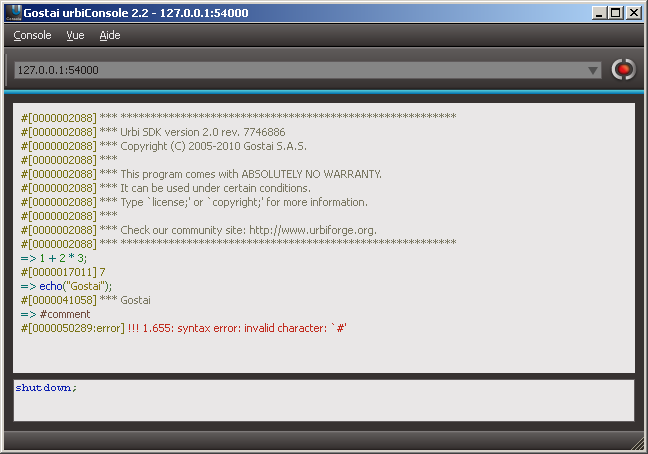
\includegraphics[width=.8\linewidth]{img/gostai-console}
\end{center}

The program \command{urbi-send} (see \autoref{sec:tools:urbi-send}) provides
a nice interface to send batches of instructions (and/or files) to a running
server.

\begin{shell}[alsolanguage={[interactive]urbiscript}]
$ urbi-send -P 54000 -e "1+2*3;" -Q
[00018032] 7
# Have the server shutdown;
$ urbi-send -P 54000 -e "shutdown;"
\end{shell}

\medskip

You can now send commands to your \urbi server. If at any point you get
lost, or want a fresh start, you can simply close and reopen your connection
to the server to get a clean environment.  In some cases, particularly if
you made global changes in the environment, it is simpler to start anew:
shut your current server down using the command \lstinline{shutdown}, and
spawn a new one. In interactive mode you can also use the shortcut sequence
\key{Ctrl-D}, like in many other interpreters.

In case of a foreground task preventing you to execute other commands, you
can use \key{Ctrl-C} to kill the foreground task, clear queued commands and
restore interactive mode.

\medskip

You are now ready to proceed to the \us tutorial: see \autoref{part:tut}.

Enjoy!

%%% Local Variables:
%%% mode: latex
%%% TeX-master: "urbi-sdk"
%%% ispell-dictionary: "american"
%%% ispell-personal-dictionary: "urbi.dict"
%%% fill-column: 76
%%% End:


%%% Keep sync with introduction.tex.
%% Copyright (C) 2010, Gostai S.A.S.
%%
%% This software is provided "as is" without warranty of any kind,
%% either expressed or implied, including but not limited to the
%% implied warranties of fitness for a particular purpose.
%%
%% See the LICENSE file for more information.

\section{UObject}

UObject is used by the \lstinline|UObject| API (see
\autoref{part:uobject}) to represent a bound \Cxx instance.

All the UObjects are copied under an unique name as slots of
\lstinline{uobjects}.

\subsection{Prototypes}
\begin{refObjects}
\item[Object]
\end{refObjects}

\subsection{Slots}

\begin{urbiscriptapi}
\item[__uobjectName]%
  Unique name assigned to this object. This is also the slot name of
  \refSlot[Global]{uobjects} containing this \lstinline|UObject|.
\end{urbiscriptapi}

%%% Local Variables:
%%% mode: latex
%%% TeX-master: "../urbi-sdk"
%%% ispell-dictionary: "american"
%%% ispell-personal-dictionary: "../urbi.dict"
%%% fill-column: 76
%%% End:

%% Copyright (C) 2009-2010, Gostai S.A.S.
%%
%% This software is provided "as is" without warranty of any kind,
%% either expressed or implied, including but not limited to the
%% implied warranties of fitness for a particular purpose.
%%
%% See the LICENSE file for more information.

\part{\us User Manual}
\label{part:tut}

%% Copyright (C) 2010, Gostai S.A.S.
%%
%% This software is provided "as is" without warranty of any kind,
%% either expressed or implied, including but not limited to the
%% implied warranties of fitness for a particular purpose.
%%
%% See the LICENSE file for more information.

\begin{partDescription}{part:specs}
  {
    %
    This part defines the specifications of the \us language version
    2.0. It defines the expected behavior from the \us interpreter,
    the standard library, and the \sdk. It can be used to check
    whether some code is valid, or browse \us or \Cxx \api for a
    desired feature. Random reading can also provide you with advanced
    knowledge or subtleties about some \us aspects.

    This part is not an \us tutorial; it is not structured in a
    progressive manner and is too detailed.  Think of it as a
    dictionary: one does not learn a foreign language by reading a
    dictionary. The \us Tutorial (\autoref{part:tut}), or the live \us
    tutorial built in the interpreter are good introductions to \us.

    This part does not aim at giving advanced programming
    techniques. Its only goal is to define the language and its
    libraries.
    %
  }
\item[sec:tools]
  Presentation and usage of the different tools available with the
  \urbi framework related to \us, such as the \urbi server, the
  command line client, \umake, \ldots

\item[sec:lang]
  Core constructs of the language and their behavior.

\item[sec:stdlib]
  Listing of all classes and methods provided in the standard library.

\item[sec:specs:ros] \urbi provides a set of tools to communicate with ROS
  (Robot Operating System). For more information about ROS, see
  \url{http://www.ros.org}.  \urbi, acting as a ROS node, is able to
  interact with the ROS world.

\item[sec:naming]
  Also known as ``The \urbi Naming Standard'': naming conventions in
  for standard hardware/software devices and components implemented as
  UObject and the corresponding slots/events to access them.

%\item[sec:sdk]
%  The \urbi software development kit that enable to
%  interact with \urbi from \Cxx.
\end{partDescription}


%%% Local Variables:
%%% mode: latex
%%% TeX-master: "../urbi-sdk"
%%% ispell-dictionary: "american"
%%% ispell-personal-dictionary: "../urbi.dict"
%%% fill-column: 76
%%% End:


%% Copyright (C) 2009-2010, Gostai S.A.S.
%%
%% This software is provided "as is" without warranty of any kind,
%% either expressed or implied, including but not limited to the
%% implied warranties of fitness for a particular purpose.
%%
%% See the LICENSE file for more information.

\chapter{First Steps}
\label{sec:tut:first}
This section introduces the most basic notions to write \us code. Some
aspects are presented only minimally.  The goal of this section is to
bootstrap yourself with the \us language, to be able to study more
in-depth examples afterward.

\section{Comments}\index{comment}

Commenting your code is crucial, so let's start by learning how to do
this in \us. Comments are ignored by the interpreter, and
can be left as documentation, reminder, \ldots \us supports \C and
\Cxx style comments:

\begin{itemize}
\item \C style comments start with \texttt{/*} and end with \texttt{*/}.
\item \Cxx style comments start with \texttt{//} and last until the
  end of the line.
\end{itemize}

\begin{urbiscript}[firstnumber=1]
1; // This is a C++ style comment.
[00000000] 1
2 + /* This is a C-style comment. */ 2;
[00000000] 4
/* Contrary to C/C++, this type of comment /* does nest */. */
3;
[00000000] 3
\end{urbiscript}


\section{Literal values}

As already seen, we can evaluate literal integers. \us supports
several other literals, such as:

\begin{description}
\item[floats] floating point numbers.
\item[strings] character strings.
\item[lists] ordered collection of values.
\item[dictionary] unordered collection of associations.
\item[nil] neutral value. Think of it as the value that fits anywhere.
\item[void] absence of value. Think of it as the value that fits nowhere.
\end{description}

These literal values can be obtained with the syntax presented below.

\begin{urbiscript}
42; // Integer literal.
[00000000] 42
3.14; // Floating point number literal.
[00000000] 3.14
"string"; // Character string literal.
[00000000] "string"
[1, 2, "a", "b"]; // List literal.
[00000000] [1, 2, "a", "b"]
["a" => 1, "b" => 2]; // Dictionary literal.
[00000000] ["a" => 1, "b" => 2]
nil;
void;
\end{urbiscript}

This listing highlights some point:
\begin{itemize}
\item Lists and Dictionaries in \us are heterogeneous. That is, one list can
  hold values of different types.
\item The printing of nil and void is empty.
\end{itemize}

\section{Function calls}

You can call functions with the classical, mathematical notation.

\begin{urbiscript}
cos(0); // Compute cosine
[00000000] 1
max(1, 3); // Get the maximum of the arguments.
[00000000] 3
max(1, 3, 4, 2);
[00000000] 4
\end{urbiscript}

Again, the result of the evaluation are printed out. You can see here
that function in \us can be variadic, that is, take different number
of arguments, such as the \lstinline{max} function. Let's now try the
\lstinline{echo} function, that prints out its argument.

\begin{urbiscript}
echo("Hello world!");
[00000000] *** Hello world!
\end{urbiscript}

The server prints out \lstinline{Hello world!}, as expected. Note that
this output is still prepended with the time stamp. Since echo returns
void, no evaluation result is printed.

\section{Variables}\index{variable}
Variables can be introduced with the \lstinline{var} keyword, given a
name and an initial value. They can be assigned new values with the
\lstinline{=} operator.

\begin{urbiscript}
var x = 42;
[00000000] 42
echo(x);
[00000000] *** 42
x = 51;
[00000000] 51
x;
[00000000] 51
\end{urbiscript}

Note that, just as in \Cxx, assignments return the (right-hand side) value, so
you can write code like ``\lstinline|x = y = 0|''. The rule for valid
identifiers is also the same as in \Cxx: they may contain alphanumeric
characters and underscores, but they may not start with a digit.

You may omit the initialization value, in which case it defaults to
\lstinline|void|.

\begin{urbiscript}
var y;
y;
// Remember, the interpreter remains silent
// because void is printed out as nothing.
// You can convince yourself that y is actually
// void with the following methods.
y.asString;
[00000000] "void"
y.isVoid;
[00000000] true
\end{urbiscript}

\section{Scopes}\index{scope}
Scopes are introduced with curly brackets (\lstinline|{}|).  They can
contain any number of statements. Variables declared in a scope only
exist within this scope.

\begin{urbiscript}
{
  var x = "test";
  echo(x);
};
[00000000] *** test
// x is no longer defined here
\end{urbiscript}

Note that the interpreter waits for the whole scope to be inputted to
evaluate it. Also note the mandatory terminating semicolon after the
closing curly bracket.

\section{Method calls}

Methods are called on objects with the dot (\lstinline{.}) notation as in
\Cxx. Method calls can be chained. Methods with no arguments don't
require the parentheses.

\begin{urbiscript}
0.cos();
[00000000] 1
"a-b-c".split("-");
[00000000] ["a", "b", "c"]
// Empty parentheses are optional
"foo".length();
[00000000] 3
"foo".length;
[00000000] 3
// Method call can be chained
"".length.cos;
[00000000] 1
\end{urbiscript}

In \lstinline|obj.method|, we say that \lstinline{obj} is the
\dfn{target}, and that we are sending him the \lstinline{method}
\dfn{message}.

\section{Function definition}

You know how to call routines, let's learn how to write
some. Functions can be declared thanks to the \lstinline{function}
keyword, followed by the comma separated, parentheses surrounded list
of formal arguments, and the body between curly brackets.

\begin{urbiscript}
// Define myFunction
function myFunction()
{
  echo("Hello world");
  echo("from my function!");
};
[00000000] function () {
[:]  echo("Hello world");
[:]  echo("from my function!");
[:]}

// Invoke it
myFunction();
[00000000] *** Hello world
[00000000] *** from my function!
\end{urbiscript}

Note the strange output after you defined the function. \us seems to
be printing the function you just typed in again. This is because
a function definition evaluates to the freshly created function.

Functions are first class citizen: they are values, just as
\lstinline{0} or \lstinline{"foobar"}.  The evaluation of a function
definition yields the new function, and as always, the interpreter
prints out the evaluation result, thus showing you the function
again:

\begin{urbiscript}
// Work in a scope.
{
  // Define f
  function f()
  {
    echo("f")
  };
  // This does not invoke f, it returns its value.
  f;
};
[00000000] function () {
[:]  echo("f")
[:]}
{
  // Define f
  function f()
  {
    echo("Hello World");
  };
  // This actually calls f
  f();
};
[00000000] *** Hello World
\end{urbiscript}

Here you can see that \lstinline{f} is actually a simple value. You can just
evaluate it to see its value, that is, its body. By adding the
parentheses, you can actually call the function. This is a difference
with methods calling, where empty parentheses are optional: method are
always evaluated, you cannot retrieve their functional value --- of
course, you can with a different construct, but that's not the point
here.

Since this output is often irrelevant, most of the time it is hidden
in this documentation using the \lstinline'|{};' trick (or even
\lstinline'|;'): when evaluating \lstinline'\var{code} | {};', the
server first evaluates \var{code}, then evaluates \lstinline'{}' and
return its value, \lstinline'void', which prints to nothing.

\begin{urbiscript}
function sum(a, b, c)
{
  return a + b + c;
} | {};
sum(20, 2, 20);
[00000000] 42
\end{urbiscript}

The \lstinline{return} keyword enables to return a value from the
function. If no \lstinline{return} statement is executed, the
evaluation of the last expression is returned.

\begin{urbiscript}
function succ(i) { i + 1 } | {};
succ(50);
[00000000] 51
\end{urbiscript}

\section{Conclusion}

You're now up and running with basic \us code, and we can dive in
details into advanced \us code.

%%% Local Variables:
%%% mode: latex
%%% TeX-master: "../urbi-sdk"
%%% ispell-dictionary: "american"
%%% ispell-personal-dictionary: "../urbi.dict"
%%% fill-column: 76
%%% End:

%% Copyright (C) 2009-2010, Gostai S.A.S.
%%
%% This software is provided "as is" without warranty of any kind,
%% either expressed or implied, including but not limited to the
%% implied warranties of fitness for a particular purpose.
%%
%% See the LICENSE file for more information.

\chapter{Basic Objects, Value Model}
\label{sec:tut:value}

In this section, we focus on \us values as objects, and study \us
by-reference values model. We won't study classes and actual objective
programming yet, these points will be presented in
\autoref{sec:tut:object}.

\section{Objects in \us}
\label{sec:tut:objects}
An object in \us is a rather simple concept: a list of slots. A
\dfn{slot} is a value associated to a name. So an \dfn{object} is a
list of slot names, each of which indexes a value --- just like a
dictionary.

\begin{urbiscript}[firstnumber=1]
// Create a fresh object with two slots.
class Foo
{
  var a = 42;
  var b = "foo";
};
[00000000] Foo
\end{urbiscript}

The \lstinline{localSlotNames} method lists the names of the slots of
an object (\refObject{Object}).

\begin{urbiscript}
// Inspect it.
Foo.localSlotNames;
[00000000] ["a", "asFoo", "b", "type"]
\end{urbiscript} % fix color $

You can get an object's slot value by using the dot (\lstinline{.})
operator on this object, followed by the name of the slot.

\begin{urbiscript}
// We now know the name of its slots. Let's see their value.
Foo.a;
[00000000] 42
Foo.b;
[00000000] "foo"
\end{urbiscript}

It's as simple as this.  The \lstinline|inspect| method provides a
convenient short-hand to discover an object (\refObject{Object}).

\begin{urbiscript}
Foo.inspect;
[00000009] *** Inspecting Foo
[00000010] *** ** Prototypes:
[00000011] ***   Object
[00000012] *** ** Local Slots:
[00000014] ***   a : Float
[00000015] ***   asFoo : Code
[00000016] ***   b : String
[00000013] ***   type : String
\end{urbiscript} % fix color $

Let's now try to build such an object. First, we want a fresh object
to work on. In \us, \lstinline{Object} is the parent type of every
object (in fact, since \us is prototype-based, \lstinline{Object} is
the uppermost prototype of every object, but we'll talk about
prototypes later). An instance of object, is an empty, neutral object,
so let's start by instantiating one with the \lstinline{clone} method
of \lstinline{Object}.

\begin{urbiscript}
// Create the o variable as a fresh object.
var o = Object.clone;
[00000000] Object_0x00000000
// Check its content
o.inspect;
[00006725] *** Inspecting Object_0x00000000
[00006725] *** ** Prototypes:
[00006726] ***   Object
[00006726] *** ** Local Slots:
\end{urbiscript}

As you can see, we obtain an empty fresh object. Note that it still
inherits from \lstinline{Object} features that all objects share, such as
the \lstinline{localSlotNames} method.

Also note how \lstinline{o} is printed out: \lstinline{Object_},
followed by an hexadecimal number. Since this object is empty, its
printing is quite generic: its type (\lstinline{Object}), and its
unique identifier (every \us object has one). Since these identifiers
are often irrelevant and might differ between two executions, they are
often filled with zeroes in this document.

We're now getting back to our empty object. We want to give it two
slots, \lstinline{a} and \lstinline{b}, with values \lstinline|42| and
\lstinline|"foo"| respectively. We can do this with the
\lstinline{setSlot} method, which takes the slot name and
its value.

\begin{urbiscript}
o.setSlot("a", 42);
[00000000] 42
o.inspect;
[00009837] *** Inspecting Object_0x00000000
[00009837] *** ** Prototypes:
[00009837] ***   Object
[00009838] *** ** Local Slots:
[00009838] ***   a : Float
\end{urbiscript}

Here we successfully created our first slot, \lstinline|a|. A good
shorthand for setting slot is using the \lstinline{var} keyword.

\begin{urbiscript}
// This is equivalent to o.setSlot("b", "foo").
var o.b = "foo";
[00000000] "foo"
o.inspect;
[00072678] *** Inspecting Object_0x00000000
[00072678] *** ** Prototypes:
[00072679] ***   Object
[00072679] *** ** Local Slots:
[00072679] ***   a : Float
[00072680] ***   b : String
\end{urbiscript}

The latter form with \lstinline{var} is preferred, but you need to know
the name of the slot at the time of writing the code. With the former
one, you can compute the slot name at execution time. Likewise, you
can read a slot with a run-time determined name with the
\lstinline{getSlot} method, which takes the slot name as
argument.  The following listing illustrates the use of
\lstinline{getSlot} and \lstinline{setSlot} to read and write slots whose
names are unknown at code-writing time.

% mefyl: FIXME: I never introduced that '+' concatenates strings.

\begin{urbiscript}
function set(object, name, value)
{
  // We have to use setSlot here, since we don't
  // know the actual name of the slot.
  return object.setSlot("x_" + name, value);
} |;
function get(object, name)
{
  // We have to use getSlot here, since we don't
  // know the actual name of the slot.
  return object.getSlot("x_" + name);
} |;
var x = Object.clone;
[00000000] Object_0x00000000
set(x, "foo", 0);
[00000000] 0
set(x, "bar", 1);
[00000000] 1
x.localSlotNames;
[00000000] ["x_bar", "x_foo"]
get(x, "foo");
[00000000] 0
get(x, "bar");
[00000000] 1
\end{urbiscript}

Right, now we can create fresh objects, create slots in them and read
them afterward, even if their name is dynamically computed, with
\lstinline{getSlot} and \lstinline{setSlot}. Now, you might wonder if
there's a method to update the value of the slot. Guess what, there's
one, and it's named\ldots \lstinline{updateSlot} (originality
award). Getting back to our \lstinline{o} object, let's try to update one
of its slots.

\begin{urbiscript}
o.a;
[00000000] 42
o.updateSlot("a", 51);
[00000000] 51
o.a;
[00000000] 51
\end{urbiscript}

Again, there's a shorthand for \lstinline{updateSlot}: operator
\lstinline{=}.

\begin{urbiscript}
o.b;
[00000000] "foo"
// Equivalent to o.updateSlot("b", "bar")
o.b = "bar";
[00000000] "bar"
o.b;
[00000000] "bar"
\end{urbiscript}

Likewise, prefer the '\lstinline{=}' notation whenever
possible, but you'll need \lstinline{updateSlot} to update a slot whose
name you don't know at code-writing time.

Note that defining the same slot twice, be it with \lstinline{setSlot} or
\lstinline{var}, is an error. The slot must be defined once with setSlot,
and subsequent writes must be done with \lstinline{updateSlot}.

\begin{urbiscript}
var o.c = 0;
[00000000] 0
// Can't redefine a slot like this
var o.c = 1;
[00000000:error] !!! slot redefinition: c
// Okay.
o.c = 1;
[00000000] 1
\end{urbiscript}

Finally, use \lstinline{removeSlot} to delete a slot from an object.

\begin{urbiscript}
o.localSlotNames;
[00000000] ["a", "b", "c"]
o.removeSlot("c");
[00000000] Object_0x00000000
o.localSlotNames;
[00000000] ["a", "b"]
\end{urbiscript}

Here we are, now you can inspect and modify objects at will. Don't
hesitate to explore \us objects you'll encounter through this
documentation like this. Last point: reading, updating or removing a
slot which does not exist is, of course, an error.

\begin{urbiscript}
o.d;
[00000000:error] !!! lookup failed: d
o.d = 0;
[00000000:error] !!! lookup failed: d
\end{urbiscript}

\section{Methods}

Methods in \us are simply object slots containing functions. We made a
little simplification earlier by saying that \lstinline|obj.slot| is
equivalent to \lstinline|obj.getSlot("slot")|: if the fetched value is
executable code such as a function, the dot form evaluates it, as
illustrated below. Inside a method, \this gives access to
the target --- as in \Cxx.  It can be omitted if there is no ambiguity
with local variables.

\begin{urbiscript}[firstnumber=1]
var o = Object.clone;
[00000000] Object_0x0
// This syntax stores the function in the 'f' slot of 'o'.
function o.f ()
{
  echo("This is f with target " + this);
  return 42;
} |;
// The slot value is the function.
o.getSlot("f");
[00000001] function () {
[:]  echo("This is f with target ".'+'(this));
[:]  return 42;
[:]}
// Huho, the function is invoked!
o.f;
[00000000] *** This is f with target Object_0x0
[00000000] 42
// The parentheses are in fact optional.
o.f();
[00000000] *** This is f with target Object_0x0
[00000000] 42
\end{urbiscript}

This was designed this way so as one can replace an attribute, such as
an integer, with a function that computes the value. This enables to
replace an attribute with a method without changing the object
interface, since the parentheses are optional.

This implies that \lstinline|getSlot| can be a better tool for object
inspection to avoid invoking slots, as shown below.

\begin{urbiscript}
// The 'empty' method of strings returns whether the string is empty.
"foo".empty;
[00000000] false
"".empty;
[00000000] true
// Using getSlot, we can fetch the function without calling it.
"".getSlot("asList");
[00000000] function () {
[:]  split("")
[:]}
\end{urbiscript}

The \lstinline|asList| function simply bounces the task to
\lstinline|split|.  Let's try \lstinline{getSlot}'ing another method:

\begin{urbiscript}
"foo".size;
[00000000] 3
"foo".getSlot("size");
[00000000] Primitive_0x0
\end{urbiscript}

The \lstinline{size} method of \refObject{String} is another type of
object: a \refObject{Primitive}. These objects are executable, like
functions, but they are actually opaque primitives implemented in
\Cxx.

\section{Everything is an object}

If you're wondering what is an object and what is not, the answer is
simple: every single bit of value you manipulate in \us is an
object, including primitive types, types themselves, functions, \ldots

\begin{urbiscript}
var x = 0;
[00000000] 0
x.localSlotNames;
[00000000] []
var x.slot = 1;
[00000000] 1
x.localSlotNames;
[00000000] ["slot"]
x.slot;
[00000000] 1
x;
[00000000] 0
\end{urbiscript}

% FIXME: I'm saying integer through this whole documentation, even
% though 42 is a float for now. But it will eventually be an integer
% (right? right?).
As you can see, integers are objects just like any other value.

\section{The \us values model}

We are now going to focus on the \us value model, that is how values
are stored and passed around. The whole point is to understand when
variables point to the same object.  For this, we introduce
\lstinline{uid}, a method that returns the target's unique identifier
--- the same one that was printed when we evaluated
\lstinline|Object.clone|.  Since uids might vary from an execution to
another, their values in this documentation are dummy, yet not null to
be able to differentiate them.

\begin{urbiscript}[firstnumber=1]
var o = Object.clone;
[00000000] Object_0x100000
o.uid;
[00000000] "0x100000"
42.uid;
[00000000] "0x200000"
42.uid;
[00000000] "0x300000"
\end{urbiscript}

% FIXME: maybe should I introduce == and other basic operator before.
Our objects have different uids, reflecting the fact that they are
different objects. Note that entering the same integer twice
(\lstinline{42} here) yields different objects. Let's introduce new
operators before diving in this concept. First the equality operator:
\lstinline{==}. This operator is the exact same as \C or \Cxx's one,
it simply returns whether its two operands are \emph{semantically}
equal. The second operator is \lstinline{===}, which is the
\emph{physical} equality operator. It returns whether its two operands
are the same object, which is equivalent to having the same uid. This
can seem a bit confusing; let's have an example.

\begin{urbiscript}
var a = 42;
[00000000] 42
var b = 42;
[00000000] 42
a == b;
[00000000] true
a === b;
[00000000] false
\end{urbiscript}

Here, the \lstinline{==} operator reports that \lstinline{a} and
\lstinline{b} are equal ---
indeed, they both evaluate to 42. Yet, the \lstinline{===} operator shows
that they are not the same object: they are two different
instances of integer objects, both equal 42.

Thanks to this operator, we can point out the fact that slots and
local variables in \us have a reference semantic. That is, when you
defining a local variable or a slot, you're not copying any value (as
you would be in \C or \Cxx), you're only making it refer to an already
existing value (as you would in \ruby or \java).

\begin{urbiscript}[firstnumber=1]
var a = 42;
[00000000] 42
var b = 42;
[00000000] 42
var c = a; // c refers to the same object as a.
[00000000] 42
// a, b and c are equal: they have the same value.
a == b && a == c;
[00000000] true
// Yet only a and c are actually the same object.
a === b;
[00000000] false
a === c;
[00000000] true
\end{urbiscript}

So here we see that \lstinline|a| and \lstinline|c| point to the same
integer, while \lstinline|b| points to a second one. This a
non-trivial fact: any modification on \lstinline|a| will affect
\lstinline|c| as well, as shown below.

\begin{urbiscript}
a.localSlotNames;
[00000000] []
b.localSlotNames;
[00000000] []
c.localSlotNames;
[00000000] []
var a.flag; // Create a slot in a.
a.localSlotNames;
[00000000] ["flag"]
b.localSlotNames;
[00000000] []
c.localSlotNames;
[00000000] ["flag"]
\end{urbiscript}

Updating slots or local variables does not update the referenced
value. It simply redirects the variable to the new given value.

\begin{urbiscript}[firstnumber=1]
var a = 42;
[00000000] 42
var b = a;
[00000000] 42
// b and a point to the same integer.
a === b;
[00000000] true
// Updating b won't change the referred value, 42,
// it makes it reference a fresh integer with value 51.
b = 51;
[00000000] 51
// Thus, a is left unchanged:
a;
[00000000] 42
\end{urbiscript}

Understanding the two latter examples is really important, to be aware
of what your variable are referring to.

Finally, function and method arguments are also passed by reference:
they can be modified by the function.

\begin{urbiscript}[firstnumber=1]
function test(arg)
{
  var arg.flag;  // add a slot in arg
  echo(arg.uid); // print its uid
} |;
var x = Object.clone;
[00000000] Object_0x1
x.uid;
[00000000] "0x1"
test(x);
[00000000] *** 0x1
x.localSlotNames;
[00000000] ["flag"]
\end{urbiscript}

Beware however that arguments are passed by reference, and the
behavior might not be what you may expected.

\begin{urbiscript}[firstnumber=1]
function test(arg)
{
  // Updates the local variable arg to refer 1.
  // Does not affect the referred value, nor the actual external argument.
  arg = 1;
} |;
var x = 0;
[00000000] 0
test(x);
[00000000] 1
// x wasn't modified
x;
[00000000] 0
\end{urbiscript}

\section{Conclusion}

You should now understand the reference semantic of local variables,
slots and arguments. It's very important to keep them in mind,
otherwise you will end up modifying variables you didn't want, or
change a copy of reference, failing to update the desired one.

%%% Local Variables:
%%% mode: latex
%%% TeX-master: "../urbi-sdk"
%%% ispell-dictionary: "american"
%%% ispell-personal-dictionary: "../urbi.dict"
%%% fill-column: 76
%%% End:

%% Copyright (C) 2009-2010, Gostai S.A.S.
%%
%% This software is provided "as is" without warranty of any kind,
%% either expressed or implied, including but not limited to the
%% implied warranties of fitness for a particular purpose.
%%
%% See the LICENSE file for more information.

\chapter{Flow Control Constructs}
\label{sec:tut:flow}

In this section, we'll introduce some flow control structures that
will prove handy later. Most of them are inspired by \C/\Cxx.

\section{if}

The \lstinline{if} construct is the same has \C/\Cxx's one. The
\lstinline{if} keyword is followed by a condition between parentheses and
an expression, and optionally the \lstinline{else} keyword and another
expression. If the condition evaluates to true, the first expression
is evaluated. Otherwise, the second expression is evaluated if
present.

\begin{urbiscript}[firstnumber=1]
if (true)
  echo("ok");
[00000000] *** ok
if (false)
  echo("ko")
else
  echo("ok");
[00000000] *** ok
\end{urbiscript}

The \lstinline|if| construct is an expression: it has a value.

\begin{urbiscript}
echo({ if (false) "a" else "b" });
[00000000] *** b
\end{urbiscript}

\section{while}

The \lstinline{while} construct is, again, the same as in \C/\Cxx. The
\lstinline{while} keyword is followed by a condition between parentheses
and an expression. If the condition evaluation is false, the
execution jumps after the while block; otherwise, the expression is
evaluated and control jumps before the while block.

% FIXME: += wasn't introduced
\begin{urbiscript}
var x = 2;
[00000000] 2
while (x < 40)
{
  x += 10;
  echo(x);
};
[00000000] *** 12
[00000000] *** 22
[00000000] *** 32
[00000000] *** 42
\end{urbiscript}

\section{for}

The \lstinline{for} keyword supports different constructs, as in
languages such as Java, \Cs, or even the forthcoming \Cxx revision.

The first construct is hardly more than syntactic sugar for a
\lstinline{while} loop.

\begin{urbiscript}
for (var x = 2; x < 40; x += 10)
  echo(x);
[00000000] *** 2
[00000000] *** 12
[00000000] *** 22
[00000000] *** 32
\end{urbiscript}

The second construct allows to iterate over members of a collection,
such as a list. The \lstinline{for} keyword, followed by
\lstinline|var|, an identifier, a colon (or \lstinline|in|), an
expression and a scope, executes the scope for every element in the
collection resulting of the evaluation of the expression, with the
variable named with the identifier referring to the list members.

\begin{urbiscript}
for (var e : [1, 2, 3]) { echo(e) };
[00000000] *** 1
[00000000] *** 2
[00000000] *** 3
\end{urbiscript}

\section{switch}

The syntax of the \lstinline|switch| construct is similar to \C/\Cxx's
one, except it works on any kind of object, not only integral
ones. Comparison is done by semantic equality (operator
\lstinline{==}). Execution will jump out of the
\lstinline|switch|-block after a case has been executed (no need to
\lstinline{break}).  Also, contrary to \Cxx, the whole construct has a
value: that of the matching \lstinline{case}.

\begin{urbiscript}
switch ("bar")
{
  case "foo":  0;
  case "bar":  1;
  case "baz":  2;
  case "qux":  3;
};
[00000000] 1
\end{urbiscript}

\section{do}
\label{section:constructs:do}

A \lstinline|do| scope is a shorthand to perform several actions on an
object.

\begin{urbiscript}
var o1 = Object.clone;
[00000000] Object_0x100000
var o1.one = 1;
[00000000] 1
var o1.two = 2;
[00000000] 2
echo(o1.uid);
[00000000] *** 0x100000
\end{urbiscript}

The same result can be obtained with a short \lstinline|do| scope,
that redirect method calls to their target, as in the listing
below. This is similar to the \pascal
``\lstinline[language=Pascal]{with}'' construct.  The value of the
\lstinline{do}-block is the target itself.

\begin{urbiscript}
var o2 = Object.clone;
[00000000] Object_0x100000
// All the message in this scope are destined to o.
do (o2)
{
  var one = 1; // var is a shortcut for the setSlot
  var two = 2; // message, so it applies on obj too.
  echo(uid);
};
[00000000] *** 0x100000
[00000000] Object_0x100000
\end{urbiscript}


%\section{Conclusion} FIXME?

%%% Local Variables:
%%% mode: latex
%%% TeX-master: "../urbi-sdk"
%%% ispell-dictionary: "american"
%%% ispell-personal-dictionary: "../urbi.dict"
%%% fill-column: 76
%%% End:

%% Copyright (C) 2009-2010, Gostai S.A.S.
%%
%% This software is provided "as is" without warranty of any kind,
%% either expressed or implied, including but not limited to the
%% implied warranties of fitness for a particular purpose.
%%
%% See the LICENSE file for more information.

\chapter{Advanced Functions and Scoping}
\label{sec:tut:function}

This section presents advanced uses of functions and scoping, as well
as their combo: lexical closures, which prove to be a very powerful
tool.

\section{Scopes as expressions}

Contrary to other languages from the \C family, scopes are
expressions: they can be used where values are expected, just as
\lstinline|1 + 1| or \lstinline|"foo"|.
They evaluate to the value of their last expression, or
\lstinline|void| if they are
empty. The following listing illustrates the use of scopes as
expressions. Note that the last semicolon inside a scope is optional.

\begin{urbiscript}[firstnumber=1]
// Scopes evaluate to the last expression they contain.
{ 1; 2; 3};
[00000000] 3
// They are expressions.
echo({1; 2; 3});
[00000000] *** 3
\end{urbiscript}

\section{Advanced scoping}

Scopes can be nested. Variables can be redefined in sub-scopes. In
this case, the inner variables hide the outer ones, as illustrated
below.

\begin{urbiscript}
var x = 0;   // Define the outer x.
[00000000] 0
{
  var x = 1; // Define an inner x.
  x = 2;     // These refer to
  echo(x);   // the inner x
};
[00000000] *** 2
x;           // This is the outer x again.
[00000000] 0
{
  x = 3;     // This is still the outer x.
  echo(x);
};
[00000000] *** 3
x;
[00000000] 3
\end{urbiscript}

\section{Local functions}

Functions can be defined anywhere local variables can --- that is,
about anywhere. These functions' visibility are limited to the scope
they're defined in, like variables. This enables for instance to write
local helper functions like ``max2'' in the example below.

\begin{urbiscript}
function max3(a, b, c) // Max of three values
{
  function max2(a, b)
  {
    if (a > b)
      return a
    else
      return b
  };
  max2(a, max2(b, c));
} | {};
\end{urbiscript}

\section{Lexical closures}

A \dfn{closure} is the capture by a function of a variable external to this
function. \us supports lexical closure: functions can refer to outer
local variables, as long as they are visible (in scope) from where
the function is defined.

\begin{urbiscript}
function printSalaries(rate)
{
  var charges = 100;
  function computeSalary(hours)
  {
    // Here rate and charges are captured
    // from the environment by closure
    rate * hours - charges
  };

  echo("Alice's salary is " + computeSalary(35));
  echo("Bob's salary is " + computeSalary(30));
} | {};
printSalaries(15);
[00000000] *** Alice's salary is 425
[00000000] *** Bob's salary is 350
\end{urbiscript}

Closures can also write to captured variables, as shown below.

% Fixme: these are not actually closures because of the toplevel ...
\begin{urbiscript}
var a = 0;
[00000000] 0
var b = 0;
[00000000] 0
function add(n)
{
  // x and y are updated by closure
  a += n;
  b += n;
  void
} | {};
add(25);
add(25);
add(1);
a;
[00000000] 51
b;
[00000000] 51
\end{urbiscript}

Closure can be really powerful tools in some situation, and they are
even more useful when combined with functional programing, as
described in \autoref{sec:tut:functional}.

%\section{Conclusion}


%%% Local Variables:
%%% mode: latex
%%% TeX-master: "../urbi-sdk"
%%% ispell-dictionary: "american"
%%% ispell-personal-dictionary: "../urbi.dict"
%%% fill-column: 76
%%% End:

%% Copyright (C) 2009-2010, Gostai S.A.S.
%%
%% This software is provided "as is" without warranty of any kind,
%% either expressed or implied, including but not limited to the
%% implied warranties of fitness for a particular purpose.
%%
%% See the LICENSE file for more information.

\section{Object}

All objects in \us must have \refObject{Object} in their
parents. \refObject{Object} is done for this purpose so that it come
with many primitives that are mandatory for all object in \us.

\subsection{Prototypes}

\begin{refObjects}
\item[Orderable]
\item[Global]
\end{refObjects}

\subsection{Construction}

Fresh object can be instantiated by cloning Object itself.

\begin{urbiscript}[firstnumber=1]
Object.new;
[00000421] Object_0x00000000
\end{urbiscript}

The keyword \lstindex{class} also allows to define objects which are
intended to serve as prototype of a family of objects, similarly to
classes in traditional object-oriented programming languages (see
\autoref{sec:tut:class}).

\begin{urbiscript}
{
  class Foo
  {
    var attr = 23;
  };
  assert
  {
    Foo.localSlotNames == ["asFoo", "attr", "type"];
    Foo.asFoo === Foo;
    Foo.attr == 23;
    Foo.type == "Foo";
  };
};
\end{urbiscript}


\subsection{Slots}

\begin{urbiscriptapi}
\item[acceptVoid]
  Return \this.  See \refObject{void} to know why.
\begin{urbiscript}
{
  var o = Object.new;
  assert(o.acceptVoid === o);
};
\end{urbiscript}


\item[addProto](<proto>)%
  Add \var{proto} into the list of prototypes of \this.
  Return \this.
\begin{urbiscript}
do (Object.new)
{
  assert
  {
    addProto(Orderable) === this;
    protos == [Orderable, Object];
  };
}|;
\end{urbiscript}

\item[allProto]
  Return a list with \this, all parents of
  \this, the parents of the parents of
  \this,\ldots
\begin{urbiassert}
123.allProtos.size == 12;
\end{urbiassert}

\item[allSlotNames]
  Deprecated alias for \refSlot{slotNames}.
\begin{urbiassert}
Object.allSlotNames == Object.slotNames;
\end{urbiassert}

\item[apply](<args>)%
  ``Invoke \this''.  The size of the argument list,
  \var{args}, must be one.  This argument is ignored.  This function
  exists for compatibility with \refSlot[Code]{apply}.
\begin{urbiassert}
Object.apply([this]) === Object;
Object.apply([1])    === Object;
\end{urbiassert}

\item[as](<type>)%
  Convert \this to \var{type}.  This is syntactic sugar for
  \lstinline|as\var{Type}| when \var{Type} is the \lstinline|type| of
  \var{type}.
\begin{urbiassert}
     12.as(Float) == 12;
   "12".as(Float) == 12;
    12.as(String) == "12";
Object.as(Object) === Object;
\end{urbiassert}

\item[asBool]
  Whether \this is ``true'', see \autoref{sec:truth}.
\begin{urbiscript}
assert
{
  Global.asBool == true;
  nil.asBool ==    false;
};
void.asBool;
[00000421:error] !!! unexpected void
\end{urbiscript}

\item[bounce](<name>)%
  Return \lstinline|this.\var{name}| transformed from a method into a
  function that takes its target (its ``\this'') as first
  and only argument.  \lstinline|this.\var{name}| must take no
  argument.
\begin{urbiassert}
{ var myCos = Object.bounce("cos"); myCos(0) }    == 0.cos;
{ var myType = bounce("type"); myType(Object); } == "Object";
{ var myType = bounce("type"); myType(3.14); }   == "Float";
\end{urbiassert}

\item[callMessage](<msg>)%
  Invoke the \refObject{CallMessage} \var{msg} on this.
%%% \begin{urbiscript}
%%% function f(var tgt, var msg, var args)
%%% {
%%%   call.target  = tgt;
%%%   call.message = msg;
%%%   call.code = tgt.getSlot(msg);
%%%   call.args    = args;
%%%   call.inspect;
%%%   tgt.callMessage(call);
%%% }|;
%%% assert
%%% {
%%%   f(Object, "type", []) == "Object.f(1, 2)";
%%%
%%% };
%%% \end{urbiscript}
\item[clone]
  Clone \this, i.e., create a fresh, empty, object, which
  sole prototype is \this.
\begin{urbiassert}
Object.clone.protos == [Object];
Object.clone.localSlotNames == [];
\end{urbiassert}

\item[cloneSlot](<from>, <to>)%
  Set the new slot \var{to} using a clone of \var{from}. This can only
  be used into the same object.

\begin{urbiscript}
var foo = Object.new |;
cloneSlot("foo", "bar") |;
assert(!(foo === bar));
\end{urbiscript}

\item[copySlot](<from>, <to>)%
  Same as \lstinline|cloneSlot|, but the slot aren't cloned, so the
  two slot are the same.
\begin{urbiscript}
var moo = Object.new |;
cloneSlot("moo", "loo") |;
assert(!(moo === loo));
\end{urbiscript}

\item[createSlot](<name>)%
  Create an empty slot (which actually means it is bound to
  \lstinline|void|) named \var{name}.  Raise an error if \var{name}
  was already defined.
\begin{urbiscript}
do (Object.new)
{
  assert(!hasLocalSlot("foo"));
  assert(createSlot("foo").isVoid);
  assert(hasLocalSlot("foo"));
}|;
\end{urbiscript}

\item[dump](<depth>)%
  Describe \this: its prototypes and slots.  The argument
  \var{depth} specifies how recursive the description is: the greater,
  the more detailed.  This method is mostly useful for debugging
  low-level issues, for a more human-readable interface, see also
  \refSlot{inspect}.
\begin{urbiscript}
do (2) { var this.attr = "foo"; this.attr->prop = "bar" }.dump(0);
[00015137] *** Float_0x240550 {
[00015137] ***   /* Special slots */
[00015137] ***   protos = Float
[00015137] ***   value = 2
[00015137] ***   /* Slots */
[00015137] ***   attr = String_0x23a750 <...>
[00015137] ***     /* Properties */
[00015137] ***     prop = String_0x23a7a0 <...>
[00015137] ***   }
do (2) { var this.attr = "foo"; this.attr->prop = "bar" }.dump(1);
[00020505] *** Float_0x240550 {
[00020505] ***   /* Special slots */
[00020505] ***   protos = Float
[00020505] ***   value = 2
[00020505] ***   /* Slots */
[00020505] ***   attr = String_0x23a750 {
[00020505] ***     /* Special slots */
[00020505] ***     protos = String
[00020505] ***     /* Slots */
[00020505] ***     }
[00020505] ***     /* Properties */
[00020505] ***     prop = String_0x239330 {
[00020505] ***       /* Special slots */
[00020505] ***       protos = String
[00020505] ***       /* Slots */
[00020505] ***       }
[00020505] ***   }
\end{urbiscript}

\item[getPeriod]
  Deprecated.  Use \refSlot[System]{period} instead.

\item[getProperty](<slotName>, <propName>)%
  Return the value of the \var{propName} property associated to the
  slot \var{slotName} if defined, \lstinline|void| otherwise.
\begin{urbiscript}
const var myPi = 3.14|;
assert
{
  getProperty("myPi", "constant");
  getProperty("myPi", "foobar").isVoid;
};
\end{urbiscript}

\item[getLocalSlot](<name>)%
  The value associated to \var{name} in \this, excluding
  its ancestors (contrary to \lstinline|getSlot|).
\begin{urbiscript}
var a = Object.new|;

// Local slot.
var a.slot = 21|;
assert
{
  a.locateSlot("slot") === a;
  a.getLocalSlot("slot") == 21;
};

// Inherited slot are not looked-up.
assert { a.locateSlot("init") == Object };
a.getLocalSlot("init");
[00041066:error] !!! lookup failed: init
\end{urbiscript}

\item[getSlot](<name>)%
  The value associated to \var{name} in \this, possibly
  after a look-up in its prototypes (contrary to
  \lstinline|getLocalSlot|).
\begin{urbiscript}
var b = Object.new|;
var b.slot = 21|;

assert
{
  // Local slot.
  b.locateSlot("slot") === b;
  b.getSlot("slot") == 21;

  // Inherited slot.
  b.locateSlot("init") === Object;
  b.getSlot("init") == Object.getSlot("init");
};

// Unknown slot.
assert { b.locateSlot("ENOENT") == nil; };
b.getSlot("ENOENT");
[00041066:error] !!! lookup failed: ENOENT
\end{urbiscript}

\item[hasLocalSlot](<slot>)%
  Whether \this features a slot \var{slot}, locally, not
  from some ancestor.  See also \refSlot{hasSlot}.
\begin{urbiscript}
class Base         { var this.base = 23; } |;
class Derive: Base { var this.derive = 43 } |;
assert(Derive.hasLocalSlot("derive"));
assert(!Derive.hasLocalSlot("base"));
\end{urbiscript}

\item[hasProperty](<slotName>, <propName>)%
  Whether the slot \var{slotName} of \this has a property
  \var{propName}.
\begin{urbiscript}
const var halfPi = pi / 2|;
assert
{
  hasProperty("halfPi", "constant");
  !hasProperty("halfPi", "foobar");
};
\end{urbiscript}

\item[hasSlot](<slot>)%
  Whether \this has the slot \var{slot}, locally, or from
  some ancestor.  See also \refSlot{hasLocalSlot}.

\begin{urbiassert}
Derive.hasSlot("derive");
Derive.hasSlot("base");
!Base.hasSlot("derive");
\end{urbiassert}

\item['$id']% fix color $

\item[inspect](<deep> = false)%
  Describe \this: its prototypes and slots, and their
  properties.  If \var{deep}, all the slots are described, not only
  the local slots. See also \refSlot{dump}.
\begin{urbiscript}
do (2) { var this.attr = "foo"; this.attr->prop = "bar"}.inspect;
[00001227] *** Inspecting 2
[00001227] *** ** Prototypes:
[00001227] ***   0
[00001227] *** ** Local Slots:
[00001228] ***   attr : String
[00001228] ***     Properties:
[00001228] ***      prop : String = "bar"
\end{urbiscript}

\item[isA](<obj>)%
  Return true if \this has \var{obj} in his parents, false
  otherwise.
\begin{urbiassert}
Float.isA(Orderable);
!(String.isA(Float));
\end{urbiassert}

\item[isNil]
  Return true if \this is \refObject{nil}, false otherwise.
\begin{urbiassert}
nil.isNil;
!(0.isNil);
\end{urbiassert}

\item[isProto]
  Return true if \this is a prototype, false otherwise;
\begin{urbiassert}
Float.isProto;
!(42.isProto);
\end{urbiassert}

\item[isVoid]
  Return true if \this is \lstinline|void|.  See
  \refObject{void}.
\begin{urbiassert}
void.isVoid;
! 42.isVoid;
\end{urbiassert}

\item[localSlotNames] Return a list with the names of the local slots of
  \this, not including those of its ancestors.  See also
  \refSlot{slotNames}.
\begin{urbiscript}
var top = Object.new|;
var top.top1 = 1|;
var top.top2 = 2|;
var bot = top.new|;
var bot.bot1 = 10|;
var bot.bot2 = 20|;
assert
{
  top.localSlotNames == ["top1", "top2"];
  bot.localSlotNames == ["bot1", "bot2"];
};
\end{urbiscript}

\item[locateSlot](<slot>)%
  Return \lstinline|nil| if \this don't have the slot
  \lstinline|slot|. Otherwise it returns the first lowest owner of
  \lstinline|slot| of \this.
\begin{urbiassert}
locateSlot("init") == Channel;
locateSlot("doesNotExist").isNil;
\end{urbiassert}

\item[print]
  Send \lstinline|print| to the \refSlot[Channel]{topLevel} channel.
\begin{urbiscript}
1.print;
[00001228] 1
[1, "12"].print;
[00001228] [1, "12"]
\end{urbiscript}

\item[protos]
  Return the list of prototypes of \this.
\begin{urbiassert}
12.protos == [0];
\end{urbiassert}

\item[properties](<slotName>)%
  Return a dictionary of the properties of slot \var{slotName}.  Raise
  an error if the slot does not exist.
\begin{urbiscript}
2.properties("foo");
[00238495:error] !!! lookup failed: foo
do (2) { var foo = "foo" }.properties("foo");
[00238501] ["constant" => false]
do (2) { var foo = "foo" ; foo->bar = "bar" }.properties("foo");
[00238502] ["bar" => "bar", "constant" => false]
\end{urbiscript}

\item[removeProperty](<slotName>, <propName>)%
  Remove the property \var{propName} from the slot \var{slotName}.
  Raise an error if the slot does not exist, do nothing if the
  property does not exist.
\begin{urbiscript}
do (2)
{
  var foo = "foo";
  foo->bar = "bar";
  removeProperty("foo", "bar");
}.properties("foo");
[00238502] ["constant" => false]

2.removeProperty("foo", "bar");
[00000072:error] !!! lookup failed: foo

do (2)
{
  var foo = "foo";
  removeProperty("foo", "bar");
}|;
\end{urbiscript}

\item[removeProto](<proto>)%
  Remove \var{proto} from the list of prototypes of \this,
  and return \this.  Do nothing if \var{proto} is not a
  prototype of \this.
\begin{urbiscript}
do (Object.new)
{
  assert
  {
    addProto(Orderable);
    removeProto(123) === this;
    protos == [Orderable, Object];
    removeProto(Orderable) === this;
    protos == [Object];
  };
}|;
\end{urbiscript}

\item[removeSlot](<slot>)%
  Remove \var{slot} from the (local) list of slots of
  \this, and return \this.  Do nothing if
  \var{slot} does not exist.
\begin{urbiscript}
{
  var base = Object.new;
  var base.slot = "base";

  var derive = Base.new;
  var derive.slot = "derive";

  do (derive)
  {
    assert
    {
      removeSlot("no such slot") === this;
      removeSlot("slot") === this;
      localSlotNames == [];
      base.slot == "base";
      removeSlot("slot") === this;
      base.slot == "base";
    };
  }|;
};
\end{urbiscript}


\item[setConstSlot]
  Like \lstinline|setSlot| but the created slot is const.
\begin{urbiscript}
assert(setConstSlot("fortyTwo", 42) == 42);
fortyTwo = 51;
[00000000:error] !!! cannot modify const slot
\end{urbiscript}

\item[setProperty](<slotName>, <propName>, <value>)%
  Set the property \var{propName} of slot \var{slotName} to
  \var{value}.  Raise an error in \var{slotName} does not exist.
  Return \var{value}.  This is what
  \lstinline|\var{slotName}->\var{propName} = \var{value}| actually
  performs.
\begin{urbiscript}
do (Object.new)
{
  var slot = "slot";
  var value = "value";
  assert
  {
    setProperty("slot", "prop", value) === value;
    "prop" in properties("slot");
    getProperty("slot", "prop") === value;
    slot->prop === value;
    setProperty("slot", "noSuchProperty", value) === value;
  };
}|;
setProperty("noSuchSlot", "prop", "12");
[00000081:error] !!! lookup failed: noSuchSlot
\end{urbiscript}


\item[setProtos](<protos>)%
  Set the list of prototypes of \this to \var{protos}.
  Return \lstinline|void|.
\begin{urbiscript}
do (Object.new)
{
  assert
  {
    protos == [Object];
    setProtos([Orderable, Object]).isVoid;
    protos == [Orderable, Object];
  };
}|;
\end{urbiscript}

\item[setSlot](<name>, <value>)%
  Create a slot \var{name} mapping to \var{value}. Raise an error if
  \var{name} was already defined.  This is what
  \lstinline|var \var{name} = \var{value}| actually performs.
\begin{urbiassert}
Object.setSlot("theObject", Object) === Object;
Object.theObject === Object;
theObject === Object;
\end{urbiassert}

  If the current job is in redefinition mode, \lstinline|setSlot| on
  an already defined slot is not an error and overwrites the slot like
  \lstinline|updateSlot| would. See the \lstinline|redefinitionMode|
  method in \refObject{System}.

\item[slotNames]
  Return a list with the slot names of \this and its
  ancestors.
\begin{urbiassert}
Object.localSlotNames
  .subset(Object.slotNames);
Object.protos.foldl(function (var r, var p) { r + p.localSlotNames },
                    [])
  .subset(Object.slotNames);
\end{urbiassert}

\item[type]%
  The name of the type of \this.  The \lstinline|class|
  construct defines this slot to the name of the class
  (\autoref{sec:tut:class}).  This is used to display the name of
  ``instances''.
\begin{urbiscript}
class Example {};
[00000081] Example
assert
{
  Example.type == "Example";
};
Example.new;
[00000081] Example_0x6fb2720
\end{urbiscript}

\item[uid]
  Returns the unique id of \this.
\begin{urbiscript}
{
  var foo = Object.new;
  var bar = Object.new;
  assert
  {
    foo.uid == foo.uid;
    foo.uid != bar.uid;
  };
};
\end{urbiscript}

\item[unacceptvoid]
  Return \this.  See \refObject{void} to know why.
\begin{urbiscript}
{
  var o = Object.new|
  assert(o.unacceptVoid === o);
};
\end{urbiscript}

%%% FIXME: \item[uobjectInit]
\item[updateSlot](<name>, <value>)%
  Map the existing slot named \var{name} to \var{value}. Raise an
  error if \var{name} was not defined.
\begin{urbiassert}
Object.setSlot("one", 1)    == 1;
Object.updateSlot("one", 2) == 2;
Object.one                  == 2;
\end{urbiassert}

\item['&&'](<that>)%
  Short-circuiting logical and. If \this evaluates to true
  evaluate and return \var{that}, otherwise return \this
  without evaluating \var{that}.
\begin{urbiassert}
(0 && "foo") == 0;
(2 && "foo") == "foo";

(""    && "foo") == "";
("foo" && "bar") == "bar";
\end{urbiassert}

\item['||'](<that>)%
  Short-circuiting logical or. If \this evaluates to false
  evaluate and return \var{that}, otherwise return \this
  without evaluating \var{that}.
\begin{urbiassert}
(0 || "foo") == "foo";
(2 ||  1/0)  == 2;

(""    || "foo") == "foo";
("foo" || 1/0)   == "foo";
\end{urbiassert}

\item \lstinline|'!'|\\
  Logical negation. If \this evaluates to false return
  \lstinline|true| and vice-versa.
\begin{urbiassert}
!1 == false;
!0 == true;

!"foo" == false;
!""    == true;
\end{urbiassert}

\item['+='](<that>)%
  Bounce to \lstinline|this '+' \var{that}|.

\item['-='](<that>)%
  Bounce to \lstinline|this '-' \var{that}|.

\item['*='](<that>)%
  Bounce to \lstinline|this '*' \var{that}|.

\item['/='](<that>)%
  Bounce to \lstinline|this '/' \var{that}|.

\item['^='](<that>)%
  Bounce to \lstinline|this '^' \var{that}|.

\item \lstinline|'%='(\var{that})|\\
  Bounce to \lstinline|this '-' \var{that}|.

\end{urbiscriptapi}

%%% Local Variables:
%%% mode: latex
%%% TeX-master: "../urbi-sdk"
%%% ispell-dictionary: "american"
%%% ispell-personal-dictionary: "../urbi.dict"
%%% fill-column: 76
%%% End:

%% Copyright (C) 2009-2010, Gostai S.A.S.
%%
%% This software is provided "as is" without warranty of any kind,
%% either expressed or implied, including but not limited to the
%% implied warranties of fitness for a particular purpose.
%%
%% See the LICENSE file for more information.

\chapter{Functional Programming}
\label{sec:tut:functional}

\us support functional programming through first class functions and
lambda expressions.

\section{First class functions}

\us has first class functions, i.e., functions are regular values,
just like integers or strings. They can be stored in variables,  passed
as arguments to other functions, and so forth. For instance, you don't need
to write
\lstinline|function object.f(){/* ... */}| to insert a function in an
object, you can simply use \lstinline{setSlot}.

% FIXME: doesn't work, toplevel, puke, etc
\begin{urbiscript}[firstnumber=1]
var o = Object.clone | {};
// Here we can use f as any regular value
o.setSlot("m1", function () { echo("Hello") }) | {};
// This is strictly equivalent
var o.m2 = function () { echo("Hello") } | {};
o.m1;
[00000000] *** Hello
o.m2;
[00000000] *** Hello
\end{urbiscript}

This enables to write powerful pieces of code, like functions that
take function as argument. For instance, consider the \lstinline{all}
function: given a list and a function, it applies the function to each
element of the list, and returns whether all calls returned true. This
enables to check very simply if all elements in a list verify a
predicate.

\begin{urbiscript}
function all(list, predicate)
{
  for (var elt : list)
    if (!predicate(elt))
      return false;
  return true;
} | {};
// Check if all elements in a list are positive.
function positive(x) { x >= 0 } | {};
all([1, 2, 3], getSlot("positive"));
[00000000] true
all([1, 2, -3], getSlot("positive"));
[00000000] false
\end{urbiscript}

It turns out that \lstinline|all| already exists: instead of
\lstinline|all(\var{list}, \var{predicate})|, use
\lstinline|\var{list}.all(\var{predicate})|, see \refObject{List}.

\section{Lambda functions}

Another nice feature is the ability to write lambda functions, which
are anonymous functions. You can create a functional value as an
expression, without naming it, with the syntax shown below.

\begin{urbiscript}
// Create an anonymous function
function (x) {x + 1} | {};
// This enable to easily pass function
// to our "all" function:
[1, 2, 3].all(function (x) { x > 0});
[00000000] true
\end{urbiscript}

In fact, the \lstinline{function} construct we saw earlier is only a
shorthand for a variable assignment.

\begin{lstlisting}
// This ...
function obj.f (/*...*/) {/*...*/};
// ... is actually a shorthand for this
var obj.f = function (/*...*/) {/* ... */};
\end{lstlisting}

% This should maybe be outside the functional section. It is also
% incomplete.
\section{Lazy arguments}

Most popular programming languages use strict arguments evaluation:
arguments are evaluated before functions are called. Other languages
use lazy evaluation: argument are evaluated by the function only when
needed. In \us, evaluation is strict by default, but you can ask a
function not to evaluate its arguments, and do it by hand. This works
by not specifying formal arguments. The function is provided with a
\lstinline{call} object that enables you to evaluate arguments.

\begin{urbiscript}
// Note the lack of formal arguments specification
function first
{
  // Evaluate only the first argument.
  call.evalArgAt(0);
} | {};
first(echo("first"), echo("second"));
[00000000] *** first
function reverse
{
  call.evalArgAt(1);
  call.evalArgAt(0);
} | {};
reverse(echo("first"), echo("second"));
[00000000] *** second
[00000000] *** first
\end{urbiscript}

A good example are logic operators. Although \Cxx is a strict
language, it uses a few logic operators. For instance, the logical and
(\lstinline{&&}) does not evaluate its right operand if the left
operand is false (the result will be false anyway).

\us logic operator mimic this behavior. The listing below shows how
one can implement such a behavior.

\begin{urbiscript}
function myAnd
{
  if (call.evalArgAt(0))
    call.evalArgAt(1)
  else
    false;
}|;

function f()
{
  echo("f executed");
  return true;
}|;

myAnd(false, f());
[00000000] false

myAnd(true, f());
[00000000] *** f executed
[00000000] true
\end{urbiscript}

%\section{Pattern matching}

%%% Local Variables:
%%% mode: latex
%%% TeX-master: "../urbi-sdk"
%%% ispell-dictionary: "american"
%%% ispell-personal-dictionary: "../urbi.dict"
%%% fill-column: 76
%%% End:

%% Copyright (C) 2009-2010, Gostai S.A.S.
%%
%% This software is provided "as is" without warranty of any kind,
%% either expressed or implied, including but not limited to the
%% implied warranties of fitness for a particular purpose.
%%
%% See the LICENSE file for more information.

\chapter{Parallelism, Concurrent Flow Control}
\label{sec:tut:concurrent}

Parallelism is a major feature of \us. So far, all we've
seen already existed in other languages --- although we tried to pick,
mix and adapt features and paradigms to create a nice scripting
language. Parallelism is one of the corner stones of its paradigm, and
what makes it so well suited to high-level scripting of interactive
agents, in fields such as robotics or \ai.

\section{Parallelism operators}

For now, we've separated our different commands with a semicolon
(\lstinline{;}). There are actually four statement separators in \us:

\begin{itemize}
\item ``\lstinline{;}'': Serialization operator. Wait for the left
  operand to finish before continuing.
\item ``\lstinline{&}'': Parallelism n-ary operator. All its operands are
  started simultaneously, and executed in parallel. The \lstinline{&} block
  itself finishes when all the operands have finished. \lstinline{&} has
  higher precedence than other separators.
\item ``\lstinline{,}'': Background operator. Its left operand is started,
  and then it proceeds immediately to its right operand.  This operator is
  bound to scopes: when used inside a scope, the scope itself finishes only
  when all the statements backgrounded with \samp{,} have finished.
\end{itemize}

The example below demonstrates the use of \lstinline{&} to launch two
functions in parallel.

\begin{urbiscript}[firstnumber=1]
function test(name)
{
  echo(name + ": 1");
  echo(name + ": 2");
  echo(name + ": 3");
} |;
// Serialized executions
test("left") ; test ("middle"); test ("right");
[00000000] *** left: 1
[00000000] *** left: 2
[00000000] *** left: 3
[00000000] *** middle: 1
[00000000] *** middle: 2
[00000000] *** middle: 3
[00000000] *** right: 1
[00000000] *** right: 2
[00000000] *** right: 3
// Parallel execution
test("left") & test("middle") & test ("right");
[00000000] *** left: 1
[00000000] *** middle: 1
[00000000] *** right: 1
[00000000] *** left: 2
[00000000] *** middle: 2
[00000000] *** right: 2
[00000000] *** left: 3
[00000000] *** middle: 3
[00000000] *** right: 3
\end{urbiscript}

In this test, we see that the \lstinline{&} runs its operands
simultaneously.

The difference between ``\lstinline{&}'' and ``\lstinline{,}'' is
rather subtle:

\begin{itemize}
\item In the top level, no operand of a job will start ``\lstinline{&}''
  until all are known.  So if you send a line ending with ``\lstinline{&}'',
  the system will wait for the right operand (in fact, it will wait for a
  ``\lstinline{,}'' or a ``\lstinline{;}'') before firing its left operand.
  A statement ending with ``\lstinline{,}'' will be fired immediately.
\item Execution is blocked after a ``\lstinline{&}'' group until all
  its children have finished.
\end{itemize}

\begin{urbiscript}[firstnumber=1]
function test(name)
{
  echo(name + ": 1");
  echo(name + ": 2");
  echo(name + ": 3");
} | {};
// Run test and echo("right") in parallel,
// and wait until both are done before continuing
test("left") & echo("right"); echo("done");
[00000000] *** left: 1
[00000000] *** right
[00000000] *** left: 2
[00000000] *** left: 3
[00000000] *** done
// Run test in background, then both echos without waiting.
test("left") , echo("right"); echo("done");
[00000000] *** left: 1
[00000000] *** right
[00000000] *** left: 2
[00000000] *** done
[00000000] *** left: 3
\end{urbiscript}

That's about all there is to say about these operators. Although
they're rather simple, they are really powerful and enables you to
include parallelism anywhere at no syntactical cost.

\section{Detach}

The \lstindex{Control.detach} function backgrounds the execution of
its argument. Its behavior is the same as the comma (\lstinline{,})
operator, except that the execution is completely detached, and not
waited for at the end of the scope.

\begin{urbiscript}[firstnumber=1]
function test()
{
  // Wait for one second, and echo "foo".
  detach({sleep(1s); echo("foo")});
}|;
test();
echo("Not blocked");
[00000000] Job<shell_4>
[00000000] *** Not blocked
sleep(2s);
echo("End of sleep");
[00001000] *** foo
[00002000] *** End of sleep
\end{urbiscript}

\section{Tags for parallel control flows}
\label{sec:tut:tags}

A \refObject{Tag} is a multipurpose code execution control and instrumentation
feature. Any chunk of code can be tagged, by preceding it with a tag
and a colon (\lstinline{:}). Tag can be created with
\lstinline|Tag.new(\var{name})|.  Naming tags is optional, yet it's
a good idea since it will be used for many features. The example below
illustrates how to tag chunks of code.

\begin{urbiscript}[firstnumber=1]
// Create a new tag
var mytag = Tag.new("name");
[00000000] Tag<name>
// Tag the evaluation of 42
mytag: 42;
[00000000] 42
// Tag the evaluation of a block.
mytag: { "foo"; 51 };
[00000000] 51
// Tag a function call.
mytag: echo("tagged");
[00000000] *** tagged
\end{urbiscript}

You can use tags that were not declared previously, they will be created
implicitly (see below). However, this is not recommended since
tags will be created in a global scope, the \lstinline{Tag} object. This
feature can be used when inputting test code in the top level to avoid
bothering to declare each tag, yet it is considered poor
practice in regular code.

\begin{urbiscript}[firstnumber=1]
// Since mytag is not declared, this will first do:
// var Tag.mytag = Tag.new("mytag");
mytag : 42;
[00000000] 42
\end{urbiscript}

So you can tag code, yet what's the use? One of the primary purpose of
tags is to be able to control the execution of code running in
parallel. Tags have a few control methods (see \refObject{Tag}):

\begin{description}
\item[freeze] Suspend execution of all tagged code.
\item[unfreeze] Resume execution of previously frozen code.
\item[stop] Stop the execution of the tagged code. The flows of
  execution that where stopped jump immediately at the end of the
  tagged block.
\item[block] Block the execution of the tagged code, that is:
  \begin{itemize}
  \item Stop it.
  \item When an execution flow encounters the tagged block, it simply
    skips it.
  \end{itemize}
  You can think of \lstinline{block} like a permanent \lstinline{stop}.
\item[unblock] Stop blocking the tagged code.
\end{description}

The three following examples illustrate these features.

\begin{urbiscript}[firstnumber=1]
// Launch in background (using the comma) code that prints "ping"
// every second.  Tag it to keep control over it.
mytag:
  every (1s)
    echo("ping"),
sleep(2.5s);
[00000000] *** ping
[00001000] *** ping
[00002000] *** ping
// Suspend execution
mytag.freeze;
// No printing anymore
sleep(1s);
// Resume execution
mytag.unfreeze;
sleep(1s);
[00007000] *** ping
\end{urbiscript}

\begin{urbiscript}[firstnumber=1]
// Now, we print out a message when we get out of the tag.
{
  mytag:
    every (1s)
      echo("ping");
  // Execution flow jumps here if mytag is stopped.
  echo("Background job stopped")|
},
sleep(2.5s);
[00000000] *** ping
[00001000] *** ping
[00002000] *** ping
// Stop the tag
mytag.stop;
[00002500] *** Background job stopped
// Our background job finished.
// Unfreezing the tag has no effect.
mytag.unfreeze;
\end{urbiscript}

\begin{urbiscript}[firstnumber=1]
// Now, print out a message when we get out of the tag.
loop
{
  echo("ping"); sleep(1s);
  mytag: { echo("pong"); sleep(1s); };
},
sleep(3.5s);
[00000000] *** ping
[00001000] *** pong
[00002000] *** ping
[00003000] *** pong

// Block printing of pong.
mytag.block;
sleep(3s);

// The second half of the while isn't executed anymore.
[00004000] *** ping
[00005000] *** ping
[00006000] *** ping

// Reactivate pong
mytag.unblock;
sleep(3.5s);
[00008000] *** pong
[00009000] *** ping
[00010000] *** pong
[00011000] *** ping
\end{urbiscript}

\section{Advanced example with parallelism and tags}

In this section, we implement a more advanced example with
parallelism.

The listing below presents how to implement a \lstinline{timeOut}
function, that takes code to execute and a timeout as arguments. It
executes the code, and returns its value. However, if the code
execution takes longer than the given timeout, it aborts it, prints
\lstinline|"Timeout!"| and returns \lstinline|void|. In this example, we use:

\begin{itemize}
\item Lazy evaluation, since we want to delay the execution of the
  given code, to keep control on it.
\item Concurrency operators, to launch a timeout job in background.
\end{itemize}

% FIXME: doesn't work (inner return)
\begin{urbiscript}[firstnumber=1]
// timeout (Code, Duration).
function timeOut
{
  // In background, launch a timeout job that waits
  // for the given duration before aborting the function.
  // call.evalArgAt(1) is the second argument, the duration.
  {
    sleep(call.evalArgAt(1));
    echo("Timeout!");
    return;
  },
  // Run the Code and return its value.
  return call.evalArgAt(0);
} |;
timeOut({sleep(1s); echo("On time"); 42}, 2s);
[00000000] *** On time
[00000000] 42
timeOut({sleep(2s); echo("On time"); 42}, 1s);
[00000000] *** Timeout!
\end{urbiscript}

% FIXME: add example with tags

% Add chronograms

%%% Local Variables:
%%% mode: latex
%%% TeX-master: "../urbi-sdk"
%%% ispell-dictionary: "american"
%%% ispell-personal-dictionary: "../urbi.dict"
%%% fill-column: 76
%%% End:

%% Copyright (C) 2009-2010, Gostai S.A.S.
%%
%% This software is provided "as is" without warranty of any kind,
%% either expressed or implied, including but not limited to the
%% implied warranties of fitness for a particular purpose.
%%
%% See the LICENSE file for more information.

\chapter{Event-based Programming}
\label{sec:tut:event-prog}

When dealing with highly interactive agent programming, sequential
programming is inconvenient. We want to react to external, random
events, not execute code linearly with a predefined flow. \us has a
strong support for event-based programming.

\section{Event related constructs}

The first construct we will study is the \lstinline|at| keyword. Given
a condition, and an expression, \lstinline|at| will evaluate the
expression every time the condition becomes true. That is,
when a rising edge occurs on the condition.

\begin{urbiscript}[firstnumber=1]
var x = 0;
[00000000] 0
at (x > 5)
  echo("ping");
x = 5;
[00000000] 5
// This triggers the event
x = 6;
[00000000] 6
[00000000] *** ping
// Does not trigger, since the condition is already true.
x = 7;
[00000000] 7
// The condition becomes false here.
x = 3;
[00000000] 3

x = 10;
[00000000] 10
[00000000] *** ping
\end{urbiscript}

An \lstinline|onleave| block can be appended to execute an expression
when the expression \emph{becomes} false --- that is, on falling edges.

\begin{urbiscript}[firstnumber=1]
var x = false;
[00000000] false
at (x)
  echo("x")
onleave
  echo("!x");
x = true;
[00000000] true
[00000000] *** x
x = false;
[00000000] false
[00000000] *** !x
\end{urbiscript}

See \autoref{sec:lang:at} for more details on \lstinline|at|
statements.

The \lstinline|whenever| construct is similar to \lstinline|at|,
except the expression evaluation is systematically restarted when it
finishes as long as the condition stands true.

\begin{urbiscript}[firstnumber=1]
var x = false;
[00000000] false
whenever (x)
{
  echo("ping");
  sleep(1s);
};
x = true;
[00000000] true
sleep(3s);
// Whenever keeps triggering
[00000000] *** ping
[00001000] *** ping
[00002000] *** ping
x = false;
[00002000] false
// Whenever stops triggering
\end{urbiscript}

Just like \lstinline|at| has \lstinline|onleave|, \lstinline|whenever|
has \lstinline|else|: the given expression is evaluated as long as the
condition is false.

\begin{urbiscript}[firstnumber=1]
var x = false;
[00002000] false
whenever (x)
{
  echo("ping");
  sleep(1s);
}
else
{
  echo("pong");
  sleep(1s);
};
sleep (3s);
[00000000] *** pong
[00001000] *** pong
[00002000] *** pong
x = true;
[00003000] true
sleep (3s);
[00003000] *** ping
[00004000] *** ping
[00005000] *** ping
x = false;
[00006000] false
sleep (2s);
[00006000] *** pong
[00007000] *** pong
\end{urbiscript}

\section{Events}
\label{sec:tut:events}
\us enables you to define events, that can be caught with the \lstinline|at|
and \lstinline|whenever| constructs we saw earlier. You can create events by
cloning the \refObject{Event} prototype. They can then be emitted with the
\lstinline|!| keyword.

\begin{urbiscript}[firstnumber=1]
var myEvent = Event.new;
[00000000] Event_0x0
at (myEvent?)
  echo("ping");
myEvent!;
[00000000] *** ping
// events work well with parallelism
myEvent! & myEvent!;
[00000000] *** ping
[00000000] *** ping
\end{urbiscript}

Both \lstinline|at| and \lstinline|whenever| have the same behavior on
punctual events. However, if you emit an event for a given duration,
\lstinline|whenever| will keep triggering for this duration, contrary to
\lstinline|at|.

% FIXME: sleep(1s) is required at the end to make this test pass ...
\begin{urbiunchecked}[firstnumber=1]
var myEvent = Event.new;
[00000000] Event_0x0
whenever (myEvent?)
{
  echo("ping (whenever)")|
  sleep(200ms)
};
at (myEvent?)
{
  echo("ping (at)")|
  sleep(200ms)
};
// Emit myEvent for .3 second.
myEvent! ~ 300ms;
[00000000] *** ping (whenever)
[00000100] *** ping (whenever)
[00000000] *** ping (at)
\end{urbiunchecked}

%\section{Valued events}

%%% Local Variables:
%%% mode: latex
%%% TeX-master: "../urbi-sdk"
%%% ispell-dictionary: "american"
%%% ispell-personal-dictionary: "../urbi.dict"
%%% fill-column: 76
%%% End:

%% Copyright (C) 2010, Gostai S.A.S.
%%
%% This software is provided "as is" without warranty of any kind,
%% either expressed or implied, including but not limited to the
%% implied warranties of fitness for a particular purpose.
%%
%% See the LICENSE file for more information.

\chapter{Communication with ROS}
\setHtmlFileName{ros}
\label{sec:specs:ros}

This chapter is not an introduction to using ROS from \urbi, see
\autoref{sec:tut:ros} for a tutorial.

\urbi provides a set of tools to communicate with ROS (Robot Operating
System). For more information about ROS, please refer to
\url{http://www.ros.org}.  \urbi, acting as a ROS node, is able to interact
with the ROS world.


\paragraph{Requirements}

You need to have installed ROS (possibly a recent version), and compiled all
of the common ROS tools (\command{rxconsole}, \command{roscore},
\command{roscpp}, \ldots).

You also need to have a few environment variables set, normally provided
with ROS installation: \env{ROS\_ROOT}, \env{ROS\_MASTER\_URI} and
\env{ROS\_PACKAGE\_PATH}.


\paragraph{Usage}

The classes are implemented as uobjects (see \autoref{part:uobject}):
\refObject{Ros.Service}, \refObject{Ros.Topic}, and \refObject{Ros}.

This module is loaded automatically if \env{ROS\_ROOT} is set  in
your environment. If \command{roscore} is not launched, you will be noticed
by a warning and \urbi will check regularly for \command{roscore}.

If for any reason you need to load this module manually, use:
\begin{urbiunchecked}
loadModule("urbi/ros");
\end{urbiunchecked}


\section{Ros}
\defObject{Ros}

This object provides some handy tools to know the status of \command{roscore},
to list the different nodes, topics, services, \ldots.  It also serves as a
namespace entry point for ROS entities, such as \refObject{Ros.Topic} and so
forth.

\subsection{Construction}

There is no construction, since this class only provides a set of tools
related to ROS in general, or the current node (which is unique per instance
of \urbi).

\subsection{Slots}

\begin{urbiscriptapi}
\item[checkMaster]
  Whether \command{roscore} is accessible.

\item[name] The name of the current node associated with \urbi (as a
  string).  The name of an \urbi node is generally composed of
  \file{/urbi\_+random} sequence.

\item[nodes]%
  A dictionary containing all the nodes known by \command{roscore}. Each key
  of the dictionary is a node name. The associated value is an other
  dictionary, with the following keys: \lstinline{publish},
  \lstinline{subscribe}, \lstinline{services}.  Each of these keys is
  associated with a list of topics or services.
\begin{urbiassert}
"/rosout" in Ros.nodes;
Ros.name in Ros.nodes;
\end{urbiassert}


\item[Service]%
  The \refObject{Ros.Service} class.

\item[services]%
  A dictionary containing all the services known by \command{roscore}. Each
  key is the name of a service, and the associated value is a list of nodes
  that provide this service.
\begin{urbiscript}
//#roscore
var services = Ros.services|
var name = Ros.name|;
assert
{
         "/rosout/get_loggers" in services;
    "/rosout/set_logger_level" in services;
       (name + "/get_loggers") in services;
  (name + "/set_logger_level") in services;
};
\end{urbiscript}

\item[Topic]%
  The \refObject{Ros.Topic} class.

\item[topics]%
  A dictionary containing all the topics advertised to
  \command{roscore}. Each key is the name of a topic, and the associated
  value is an other dictionary, with the following keys:
  \lstinline{subscribers}, \lstinline{publishers}, \lstinline{type}.
\begin{urbiscript}
var topics = Ros.topics|;
topics.keys;
[03316144] ["/rosout_agg"]
topics["/rosout_agg"];
[03325634] ["publishers" => ["/rosout"], "subscribers" => [], "type" => "roslib/Log"]
\end{urbiscript}
\end{urbiscriptapi}


\section{Ros.Topic}
\defObject{Ros.Topic}

This \UObject provides a handy way to communicate through ROS topics, by
subscribing to existent topics or advertising to them.

\subsection{Construction}

To create a new topic, call \lstinline{Ros.topic.new} with a string (the
name of the topic you want to subscribe to / advertise on).

The topic name can only contain alphanumerical characters, \samp{/} and
\samp{\_}, and cannot be empty.  If the topic name is invalid, an exception
is thrown and the topic is not created.

Until you decide what you want to do with your topic (\refSlot{subscribe} or
\refSlot{advertise}), you are free to call \lstinline{init} to change its
name.


\subsection{Slots}

Some slots on this \UObject have no interest once the type of instance is
determined. For example, you cannot call unsubscribe if you advertise, and
in the same way you cannot call publish if you subscribed to a topic.

\subsubsection{Common}

\begin{urbiscriptapi}

\item[name]%
  The name of the topic you provided in \lstinline{init}.
\begin{urbiscript}
Ros.Topic.new("/test").name;
[00011644] "/test"
\end{urbiscript}


\item[subscriberCount]%
  The number of subscribers for the topic given in \lstinline{init}; 0 if
  the topic is not registered.

\item[structure]%
  Once \refSlot{advertise} or \refSlot{subscribe} has been called, this slot
  contains a template of the message type, with default values for each type
  (empty strings, zeros, \ldots). This template is made of
  \refObject[s]{Dictionary}.
\begin{urbiscript}
var logTopic = Ros.Topic.new("/rosout_agg")|
logTopic.subscribe|;
logTopic.structure.keys;
[00133519] ["file", "function", "header", "level", "line", "msg", "name", "topics"]
\end{urbiscript}
\end{urbiscriptapi}


\subsubsection{Subscription}

\begin{urbiscriptapi}

\item[subscribe]%
  Subscribe to the provided topic. Throw an exception it doesn't exist, or
  if the type advertised by ROS for this topic does not exist.  From the
  call of this method, a direct connection is made between the advertiser
  and the subscriber which starts deserializing the received messages.

\item[unsubscribe]%
  Unsubscribe from a previously subscribed channel, and set the state of the
  instance as if \lstinline{init} was called but not subscribe.

\item[onMessage]%
  Event triggered when a new message is received from a subscribed channel,
  the payload of this event contains the message.

\begin{urbiunchecked}
var t = Ros.Topic.new("/test")|;
msg: at (t.onMessage?(var m)) echo(m);
t.subscribe;
\end{urbiunchecked}
\end{urbiscriptapi}


\subsubsection{Advertising}

\begin{urbiscriptapi}

\item[advertise](<type>)%
  Tells ROS that this node will advertise on the topic given in
  \lstinline{init}, with the type \var{type}. \var{type} must be a valid ROS
  type, such as \samp{roslib/Log}. If \var{type} is an empty string, the
  method will try to check whether a node is already advertising on this
  topic, and its type.
\begin{urbiscript}
var stringPub = Ros.Topic.new("/mytest")|;
stringPub.advertise("std_msgs/String");
stringPub.structure;
[00670809] ["data" => ""]
\end{urbiscript}


\item[onConnect](<name>)%
  This event is triggered when the current instance is advertising on a
  topic and a node subscribes to this topic. The payload \var{name} is the
  name of the node that subscribed.
\begin{urbiunchecked}
var p = Ros.Topic.new("/test/publisher")|;
con: at (p.onConnect?(var n))
  echo(n + " has subscribed to " + p.name);
p.advertise("roslib/Log");
\end{urbiunchecked}

\item[onDisconnect](<name>)%
  This event is triggered when the current instance is advertising on a
  topic, and a node unsubscribes from this topic. The payload is the name of
  the node that unsubscribed.

\item[publish](<message>)%
  Publish \var{message} to the current topic. This method is usable only if
  \refSlot{advertise} was called. The message must follow the same structure
  as the one in the slot \lstinline{structure}, or it will throw an
  exception telling which key is missing / wrong in the dictionary.

\item['<<'](<message>)%
  An alias for \refSlot{publish}.
\begin{urbiunchecked}
stringPub << ["data" => "Hello world!"];
\end{urbiunchecked}


\item[unadvertise]%
  Tells ROS that we stop publishing on this topic. The \UObject then gets back
  to a state where it could call \lstinline{init}, \refSlot{subscribe} or
  \refSlot{advertise}.
\end{urbiscriptapi}


\subsection{Example}

This is a typical example of the creation of a publisher, a subscriber, and
message transmission between both of them.

First we need to declare our Publisher, the topic name is \file{/example},
and the type of message that will be sent on this topic is
\samp{std\_msgs/String}. This type contains a single field called
\samp{data}, holding a string.  We also set up handlers for
\refSlot{onConnect} and \refSlot{onDisconnect} to be noticed when someone
subscribes to us.

\begin{urbiscript}
var publisher = Ros.Topic.new("/example")|
con: at (publisher.onConnect?(var name))
  echo(name[0,5] + " is now listening on " + publisher.name);
dcon: at (publisher.onDisconnect?(var name))
  echo(name[0,5] + " is no longer listening on " + publisher.name);
publisher.advertise("std_msgs/String");
\end{urbiscript}

Then we subscribe to the freshly created topic, and for each message, we
display the \samp{data} section (which is the content of the
message). Thanks to the previous \lstinline{at} above, a message is
displayed at subscription time.

\begin{urbiscript}
var subscriber = Ros.Topic.new("/example")|
msg: at (subscriber.onMessage?(var m))
  echo(m["data"]);
subscriber.subscribe;
[00026580] *** /urbi is now listening on /example

// The types should be the same, ensure that.
assert { subscriber.structure == publisher.structure };
\end{urbiscript}

\begin{comment}
\begin{urbiscript}
// A small delay to let the "is now listening" message arrives
// before the next interaction.
sleep(500ms);
\end{urbiscript}
\end{comment}

Now we can send a message, and get it back through the at in the section
above. To do this we first copy the template structure and then fill the
field \samp{data} with our message.

\begin{urbiscript}
var message = publisher.structure.new;
[00098963] ["data" => ""]
message["data"] = "Hello world!"|;

// publish the message.
publisher << message;
// Leave some time to asynchronous communications before shutting down.
sleep(200ms);
[00098964] *** Hello world!

subscriber.unsubscribe;
[00252566] *** /urbi is no longer listening on /example
\end{urbiscript}



\section{Ros.Service}
\defObject{Ros.Service}

This \UObject provides a handy way to call services provided by other ROS
nodes.


\subsection{Construction}

To create a new instance of this object, call \lstinline{Ros.Service.new}
with a string representing which service you want to use, and a Boolean
stating whether the connection between you and the service provider should
be kept opened (pass \lstinline{true} for better performances on multiple
requests).

The service name can only contain alphanumerical characters, \samp{/},
\samp{\_}, and cannot be empty. If the service name is invalid, an exception
is thrown, and the object is not created.

Then if the service does not exist, an other exception is thrown. Since the
initialization is asynchronous internally, you need to wait for
\lstinline|\var{service}.initialized| to be true to be able to call
\lstinline{request}.


\subsection{Slots}

\begin{urbiscriptapi}

\item[initialized]%
  Boolean.  Whether the method \var{request} is ready to be called, and
  whether \refSlot{resStruct} and \refSlot{reqStruct} are filled.
\begin{urbiscript}
var logService = Ros.Service.new("/rosout/get_loggers", false)|;
waituntil(logService.initialized);
\end{urbiscript}

\item[name]%
  The name of the current service.
\begin{urbiscript}
logService.name;
[00036689] "/rosout/get_loggers"
\end{urbiscript}

\item[resStruct]%
  Get the template of the response message type, with default values for
  each type (empty strings, zeros, \ldots). This template is made of
  dictionaries.
\begin{urbiscript}
logService.resStruct;
[00029399] ["loggers" => []]
\end{urbiscript}

\item[reqStruct]%
  Get the template of the request message type, with default values for
  each type (empty strings, zeros, \ldots). This template is made of
  dictionaries.
\begin{urbiscript}
logService.reqStruct;
[00029399] [ => ]
\end{urbiscript}


\item[request](<req>)%
  Synchronous call to the service, providing \var{req} as your request
  (following the structure of \refSlot{reqStruct}). The returned value is a
  dictionary following the structure of \refSlot{resStruct}, containing the
  response to your request.
\begin{urbiscript}
for (var item in logService.request([=>])["loggers"])
  echo(item);
[00236349] *** ["level" => "INFO", "name" => "ros"]
[00236349] *** ["level" => "INFO", "name" => "ros.roscpp"]
[00236350] *** ["level" => "WARN", "name" => "ros.roscpp.superdebug"]
[00236350] *** ["level" => "DEBUG", "name" => "roscpp_internal"]
\end{urbiscript}

\end{urbiscriptapi}

%%% Local Variables:
%%% mode: latex
%%% TeX-master: "../urbi-sdk"
%%% ispell-dictionary: "american"
%%% ispell-personal-dictionary: "../urbi.dict"
%%% fill-column: 76
%%% End:


%%% Local Variables:
%%% mode: latex
%%% TeX-master: "../urbi-sdk"
%%% ispell-dictionary: "american"
%%% ispell-personal-dictionary: "../urbi.dict"
%%% fill-column: 76
%%% End:

%% Copyright (C) 2010, Gostai S.A.S.
%%
%% This software is provided "as is" without warranty of any kind,
%% either expressed or implied, including but not limited to the
%% implied warranties of fitness for a particular purpose.
%%
%% See the LICENSE file for more information.

\part{Guidelines and Cook Books}
\label{part:guide}

%% Copyright (C) 2010, Gostai S.A.S.
%%
%% This software is provided "as is" without warranty of any kind,
%% either expressed or implied, including but not limited to the
%% implied warranties of fitness for a particular purpose.
%%
%% See the LICENSE file for more information.

\begin{partDescription}{part:specs}
  {
    %
    This part defines the specifications of the \us language version
    2.0. It defines the expected behavior from the \us interpreter,
    the standard library, and the \sdk. It can be used to check
    whether some code is valid, or browse \us or \Cxx \api for a
    desired feature. Random reading can also provide you with advanced
    knowledge or subtleties about some \us aspects.

    This part is not an \us tutorial; it is not structured in a
    progressive manner and is too detailed.  Think of it as a
    dictionary: one does not learn a foreign language by reading a
    dictionary. The \us Tutorial (\autoref{part:tut}), or the live \us
    tutorial built in the interpreter are good introductions to \us.

    This part does not aim at giving advanced programming
    techniques. Its only goal is to define the language and its
    libraries.
    %
  }
\item[sec:tools]
  Presentation and usage of the different tools available with the
  \urbi framework related to \us, such as the \urbi server, the
  command line client, \umake, \ldots

\item[sec:lang]
  Core constructs of the language and their behavior.

\item[sec:stdlib]
  Listing of all classes and methods provided in the standard library.

\item[sec:specs:ros] \urbi provides a set of tools to communicate with ROS
  (Robot Operating System). For more information about ROS, see
  \url{http://www.ros.org}.  \urbi, acting as a ROS node, is able to
  interact with the ROS world.

\item[sec:naming]
  Also known as ``The \urbi Naming Standard'': naming conventions in
  for standard hardware/software devices and components implemented as
  UObject and the corresponding slots/events to access them.

%\item[sec:sdk]
%  The \urbi software development kit that enable to
%  interact with \urbi from \Cxx.
\end{partDescription}


%%% Local Variables:
%%% mode: latex
%%% TeX-master: "../urbi-sdk"
%%% ispell-dictionary: "american"
%%% ispell-personal-dictionary: "../urbi.dict"
%%% fill-column: 76
%%% End:


%% Copyright (C) 2009-2010, Gostai S.A.S.
%%
%% This software is provided "as is" without warranty of any kind,
%% either expressed or implied, including but not limited to the
%% implied warranties of fitness for a particular purpose.
%%
%% See the LICENSE file for more information.

\chapter{Installation}
\label{sec:installation}

\section{Download}

Various pre-compiled packages are provided.  They are named
\begin{center}
\file{urbi-sdk-\var{version}-\var{arch}-\var{os}-\var{compiler}.\var{ext}}
\end{center}
where
\begin{description}
\item[\var{version}] specifies the exact revision of Urbi that you are
  using.  It can be simple, \code{2.0}, or more complex,
  \code{2.0-beta3-137-g28f8880}.  In that case,
  \begin{description}
  \item[2.0] is the version of the \urbi Kernel,
  \item[beta3] designates the third pre-release,
  \item[137] is the number of changes since beta3 (not counting
    changes in sub-packages),
  \item[g28f8880] is a version control identifier, used internally to
    track the exact version that is being tested by our users.
  \end{description}
\item[\var{arch}] describes the architecture, the \acro{cpu}:
  \code{ARM}, \code{ppc}, or \code{x86}.
\item[\var{os}] is the operating system: \code{linux} for GNU/Linux,
  \code{osx} for Mac OS X, or \code{windows} for Microsoft Windows.
\item[\var{compiler}] is the tool chain used to compile the programs:
  \code{gcc4} for the GNU Compiler Collection 4.x, \code{vcxx2005} for
  Microsoft Visual \Cxx 2005, \code{vcxx2008} for Microsoft Visual
  \Cxx 2008.
\item[\var{ext}] is the package format extension.  For Unix architectures,
  \code{tar.bz2}; uncompress them with \command{tar xf \var{tarfile}}.  For
  Windows hosts, we provide zip files (\file{*.zip}) for both ``release''
  and ``debug'' flavors, and installers (for instance \file{*.exe}).  You
  are encouraged to use the installers, since in addition to installing
  headers and libraries, they also install Visual \Cxx Wizards to create
  UObjects, they take care of installing the Visual Runtime if needed, and
  they install Gostai Console and Gostai Editor.
\end{description}

\section{Install \&{} Check}
\label{sec:install:install}

The package is \dfn{relocatable}, i.e., it does not need to be put at
a specific location, nor does it need special environment variables to
be set.  It is not necessary to be a super-user to install it.  The
\dfn{root} of the package, denoted by \var{urbi-root} hereafter, is
the absolute name of the directory which contains the package.

After the install, the quickest way to test your installation is to run
the various programs.

\subsection{GNU/Linux and Mac OS X}

Decompress the package where you want to install it.  If \var{urbi-sdk-2.x}
denotes the version of Urbi SDK you downloaded (say, \var{urbi-sdk-2.x} is
\file{urbi-sdk-2.3-linux-x86-gcc4}), run something like:

\begin{shell}
$ rm -rf \var{urbi-root}
$ cd /tmp
$ tar xf \var{path-to}/\var{urbi-sdk-2.x}.tar.bz2
$ mv \var{urbi-sdk-2.x} \var{urbi-root}
\end{shell}

This directory, \var{urbi-root}, should contain \file{bin}, \file{FAQ.txt}
and so forth.  Do not move things around inside this directory.  In order to
have an easy access to the \urbi programs, set up your \env{PATH}:

\begin{shell}[style=varInString]
$ export PATH="\var{urbi-root}/bin:$PATH"
\end{shell}%$

\begin{shell}
# Check that urbi is properly set up.
$ urbi --version

# Check that urbi-launch is properly installed.
$ urbi-launch --version
# Check that urbi-launch can find its dependencies.
$ urbi-launch -- --version

# Check that Urbi can compute.
$ urbi -e '1+2*3; shutdown;'
[00000175] 7
\end{shell}%$

\subsection{Windows}

Decompress the zip file wherever you want or execute the installer.

Execute the script \file{urbi.bat}, located at the root of the
uncompressed package. It should open a terminal with an interactive
Urbi session.

\begin{cygwin}
Inputs and outputs of windows native application are buffered under Cygwin.
Thus, either running the interactive mode of Urbi or watching the output of the
server under Cygwin is not recommended.
\end{cygwin}

% FIXME: add a listing with the urbi banner under windows?

%%% Local Variables:
%%% mode: latex
%%% TeX-master: "../urbi-sdk"
%%% ispell-dictionary: "american"
%%% ispell-personal-dictionary: "../urbi.dict"
%%% fill-column: 76
%%% End:

%% Copyright (C) 2009-2010, Gostai S.A.S.
%%
%% This software is provided "as is" without warranty of any kind,
%% either expressed or implied, including but not limited to the
%% implied warranties of fitness for a particular purpose.
%%
%% See the LICENSE file for more information.

\chapter{Frequently Asked Questions}
\label{sec:faq}
\setHtmlFileName{faq}

\ifx\ifHtml\undefined\else
  \let\subsubsectionSave\subsubsection
  \let\subsubsection\faqsection
\fi

\section{Build Issues}
\label{sec:faq:build}

\subsection{Complaints about \samp{+=}}
At random places we use \samp{+=} in \command{/bin/sh} scripts, which Ash
(aka, \command{dash} and \command{sash}) does not support.  Please, use
\command{bash} or \command{zsh} instead of Ash as \command{/bin/sh}.

\subsection{error: `<anonymous>' is used uninitialized in this function}
\label{sec:faq:build:uninitialized}

If you encounter this error:

\begin{lstlisting}[language={}]
cc1plus: warnings being treated as errors
parser/ugrammar.hh: In member function \
  `void yy::parser::yypush_(const char*, int, yy::parser::symbol_type&)':
parser/ugrammar.hh:1240: error: `<anonymous>' is used uninitialized \
  in this function
parser/ugrammar.cc:1305: note: `<anonymous>' was declared here
parser/ugrammar.hh: In member function \
  `void yy::parser::yypush_(const char*, yy::parser::stack_symbol_type&)':
parser/ugrammar.hh:1240: error: `<anonymous>' is used uninitialized \
  in this function
parser/ugrammar.cc:1475: note: `<anonymous>' was declared here
\end{lstlisting}

\noindent
then you found a problem that we don't know how to resolved currently.
Downgrade from GCC-4.4 to GCC-4.3.

\subsection{AM\_LANGINFO\_CODESET}

If at bootstrap you have something like:

\begin{lstlisting}[language={}]
configure:12176: error: possibly undefined macro: AM_LANGINFO_CODESET
 If this token and others are legitimate, please use m4_pattern_allow.
 See the Autoconf documentation.
configure:12246: error: possibly undefined macro: gl_GLIBC21
\end{lstlisting}

\noindent
it probably means your Automake installation is incomplete.  See the
Automake item in \autoref{sec:build:req}.

%% \subsection{git: fatal: Needed a single revision}
%% You may experience something like this:
%%
%% \begin{shell}
%% $ git submodule update --init
%% fatal: Needed a single revision
%% Unable to find current revision in submodule path 'gnulib'
%% \end{shell}
%%
%% \noindent
%% this is the sign that the initial checkout of \file{gnulib} went
%% completely wrong (I don't know what makes this happen).  Chances are
%% that the directory exists, but is empty.  Git does not seem to be able
%% to overcome this situation, so:
%%
%% \begin{shell}
%% $ rm -rf gnulib
%% $ git submodule update --init
%% \end{shell}
%%
%% \noindent
%% et voila.

\subsection{\samp{make check} fails}

Be sure to read \autoref{sec:build:check}.  In particular, run \samp{make
  check} several times (see \autoref{sec:build:check} to know why).  If the
failures remain, please submit the \file{test-suite.log} file(s) (see
\autoref{sec:bug}).

\section{Troubleshooting}

\subsection{Error 1723: "A DLL required for this install to complete could
  not be run."}

This error is raised when you try to install a program like
\command{vcredist-x86.exe}.  This program use the ``Windows Installer''
which is probably outdated on your system.

To fix this problem, update the ``Windows Installer'' and re-start the
installation of vcredist which should no longer fail.

\subsection{When executing a program, the message ``The system cannot
  execute the specified program.'' is raised.}
\label{faq:vcredist:inst}

This library is necessary to start running any application.  Run
\file{vcredist-x86.exe} to install the missing libraries.

If you have used the \usdk installer, it is \file{vcredist-x86.exe} in
your install directory.  Otherwise download it from the Microsoft web site.
Be sure to get the one corresponding to the right Visual \Cxx version.

\subsection{When executing a program, the message ``This application has
  failed to start'' is raised.}

Same answer as \autoref{faq:vcredist:inst}.

\subsection{The server dies with ``stack exhaustion''}
Your program might be deeply recursive, or use large temporary
objects.  Use \option{--stack-size} to augment the stack size, see
\autoref{sec:tools:urbi}.

Note that one stack is allocated per ``light thread''.  This can
explain why programs that heavily rely on concurrency might succeed
where sequential programs can fail.  For instance the following
program is very likely to quickly exhaust the (single) stack.

\begin{urbiunchecked}
function consume (var num)
{
  if (num)
    consume(num - 1) | consume(num - 1)
}|;
consume (512);
\end{urbiunchecked}

But if you use \lstinline{&} instead of \lstinline{|}, then each
recursive call to \lstinline{consume} will be spawn with a fresh
stack, and therefore none will run out of stack space:

\begin{urbiunchecked}
function consume (var num)
{
  if (num)
    consume(num - 1) & consume(num - 1)
}|;
consume (512);
\end{urbiunchecked}

However your machine will run out of resources: this heavily
concurrent program aims at creating no less than $2^{513}$ threads,
about $2.68 \times 10^{156}$ (a 156-digit long number, by far larger
than the number of atoms in the observable universe, estimated to
$10^{80}$).

\subsection{'myuobject: file not found'. What can I do?}
If \command{urbi-launch} (or \command{urbi}) fails to load an UObject (a
shared library or \acro{DLL}) although the file exists, then the most
probable cause is an undefined symbol in your shared library.

\subsubsection{Getting a better diagnostic}
First, set the \env{GD\_LEVEL} environment variable (see
\autoref{sec:tools:env}) to some high level, say \code{DUMP}, to log
messages from \command{urbi-launch}.  You might notice that your library is
not exactly where you thought \command{urbi-launch} was looking at.

\subsubsection{GNU/Linux}
A libltdl quirk prevents us from displaying a more accurate error message.
You can use a tool named \command{ltrace} to obtain the exact error message.
Ltrace is a standard package on most Linux distributions.  Run it with
\samp{ltrace -C -s 1024 urbi-launch ...}, and look for lines containing
\samp{dlerror} in the output. One will contain the exact message that
occurred while trying to load your shared library.

It is also useful to use \command{ldd} to check that the dependencies of
your object are correct.  See the documentation of \command{ldd} on your
machine (\samp{man ldd}).  The following run is successful: every request
(left-hand side of \lstinline{=>}) is satisfied (by the file shown on the
right-hand side).

\begin{shell}
$ all.so
	linux-gate.so.1 =>  (0xb7fe8000)
	libstdc++.so.6 => \
          /usr/lib/gcc/i686-pc-linux-gnu/4.4.1/libstdc++.so.6 (0xb7eba000)
	libm.so.6 => /lib/libm.so.6 (0xb7e94000)
	libc.so.6 => /lib/libc.so.6 (0xb7d51000)
	libgcc_s.so.1 => \
          /usr/lib/gcc/i686-pc-linux-gnu/4.4.1/libgcc_s.so.1 (0xb7d35000)
	/lib/ld-linux.so.2 (0xb7fe9000)
\end{shell}

The following run shows a broken dependency.

\begin{shell}
# A simple C++ program.
$ echo 'int main() {}' >foo.cc

# Compile it, and depend on the libport shared library.
$ g++ foo.cc -L\var{urbi-root}/gostai/lib -lport -o foo

# Run it.
$ ./foo
./foo: error while loading shared libraries: \
  libport.so: cannot open shared object file: No such file or directory

# See that ldd is unhappy.
$ ldd foo
	linux-gate.so.1 =>  (0xb7fa4000)
	libport.so => not found
	libstdc++.so.6 => \
          /usr/lib/gcc/i686-pc-linux-gnu/4.4.1/libstdc++.so.6 (0xb7eae000)
	libm.so.6 => /lib/libm.so.6 (0xb7e88000)
	libgcc_s.so.1 => \
          /usr/lib/gcc/i686-pc-linux-gnu/4.4.1/libgcc_s.so.1 (0xb7e6c000)
	libc.so.6 => /lib/libc.so.6 (0xb7d29000)
	/lib/ld-linux.so.2 (0xb7fa5000)
\end{shell}

Notice the \samp{not found} message.  The shared object could not be loaded
because it is not found in the \dfn{runtime path}, which is the list of
directories where the system looks for shared objects to be loaded when
running a program.

You may extend your \env{LD\_LIBRARY\_PATH} to include the missing
directory.

\begin{shell}
$ export LD_LIBRARY_PATH=\var{urbi-root}/gostai/lib:$LD_LIBRARY_PATH
# Run it.
$ ./foo
\end{shell}

\subsubsection{Mac OS X}
Set the \env{DYLD\_PRINT\_LIBRARIES} environment variable to 1 to make the
shared library loader report the libraries it loads on the standard error
stream.

Use \command{otool} to check whether a shared object ``finds'' all its
dependencies.

\begin{shell}
$ otool -L all.so
all.so:
	/usr/lib/libstdc++.6.dylib \
          (compatibility version 7.0.0, current version 7.4.0)
	/usr/lib/libgcc_s.1.dylib \
          (compatibility version 1.0.0, current version 1.0.0)
	/usr/lib/libSystem.B.dylib \
          (compatibility version 1.0.0, current version 111.1.4)
\end{shell}

The following run shows a broken dependency.

\begin{shell}
# A simple C++ program.
$ echo 'int main() {}' >foo.cc

# Compile it, and depend on the libport shared library.
$ g++ foo.cc -L\var{urbi-root}/gostai/lib -lport -o foo

# Run it.
$ ./foo
dyld: Library not loaded: @loader_path/libport.dylib
  Referenced from: /private/tmp/./foo
  Reason: image not found

# See that otool is unhappy.
$ otool -L ./foo
./foo:
	@loader_path/libport.dylib \
          (compatibility version 0.0.0, current version 0.0.0)
	/usr/lib/libstdc++.6.dylib \
          (compatibility version 7.0.0, current version 7.4.0)
	/usr/lib/libgcc_s.1.dylib \
          (compatibility version 1.0.0, current version 1.0.0)
	/usr/lib/libSystem.B.dylib \
          (compatibility version 1.0.0, current version 111.1.5)
\end{shell}

The fact that the \file{libport.dylib} was not found shows by the unresolved
relative runtime-path: \samp{@loader\_path} still shows.  Use
\env{DYLD\_LIBRARY\_PATH} to specify additional directories where the system
should look for runtime dependencies.

\begin{shell}
$ DYLD_PRINT_LIBRARIES=1 \
  DYLD_LIBRARY_PATH=\var{urbi-root}/lib:$DYLD_LIBRARY_PATH \
  ./foo
dyld: loaded: /private/tmp/./foo
dyld: loaded: \var{urbi-root}/lib/libport.dylib
dyld: loaded: /usr/lib/libstdc++.6.dylib
dyld: loaded: /usr/lib/libgcc_s.1.dylib
dyld: loaded: /usr/lib/libSystem.B.dylib
dyld: loaded: \var{urbi-root}/lib/libboost_filesystem-mt.dylib
dyld: loaded: \var{urbi-root}/lib/libboost_signals-mt.dylib
dyld: loaded: \var{urbi-root}/lib/libboost_system-mt.dylib
dyld: loaded: \var{urbi-root}/lib/libboost_thread-mt.dylib
dyld: loaded: /usr/lib/system/libmathCommon.A.dylib
$
\end{shell}

\subsubsection{Windows}

If you are running Cygwin, then have a look at the following section, which
uses some of its tools.

A specific constraint, for which currently we do not have nice solutions, is
that when Windows loads a \acro{DLL}, it looks for all its dependencies
(i.e., other \acro{DLL} that are needed) in the directory from which the
program was run, or in the \env{PATH}.  There is no way, that we are aware
of, to embed in a \acro{DLL} the information about where the dependencies
are.  When trying to load a \acro{DLL} with missing dependencies, say
\file{foo.dll}, the error message will be something like ``can't open the
module'', and worse yet, if you read the detailed log messages (by setting
\env{GD\_LEVEL} to \code{DUMP} for instance) it will report ``failed with
error 126: The specified module could not be found'' although the file
\emph{is} there.

So first try to understand what are the missing dependencies.  Under
Windows, use \command{DependencyWalker} (see
\url{http://dependencywalker.com}) to check that a given \acro{DLL} finds
all its dependencies.  If some dependencies are not found either:
\begin{itemize}
\item change your \env{PATH} so that it goes via the directories that
  contain the dependencies of your \acro{DLL}s;
\item or copy these dependencies in the \file{bin/} directory of \usdk,
  since that's the directory of the program, \file{urbi-launch}.
\end{itemize}

The first approach is more tractable.  Beware that dependencies may also
have dependencies\ldots

\paragraph{Cygwin}

Use the \command{cygcheck.exe} program to check dependencies.  Beware that
you must provide a qualified path to the file.  Chances are that if

\begin{shell}
$ cygcheck foo.dll
\end{shell}

\noindent
does not work and will pretend that \file{foo.dll} does not exist (although
it's \emph{right there}), then this will work:

\begin{shell}
$ cygcheck ./foo.dll
\end{shell}

In this output, look for lines like these:

\begin{shell}
cygcheck: track_down: could not find OgreMain.dll
cygcheck: track_down: could not find OIS.dll
cygcheck: track_down: could not find libuobject-vc90.dll
\end{shell}

\noindent
and make sure that \file{OgreMain.dll}, \file{OIS.dll} and so forth are
visible in the \env{PATH} (don't be worry about \file{libuobject-vc90.dll},
\command{urbi-launch} will take care of it).  Note that when they are
finally visible from the \env{PATH}, then you can run

\begin{shell}
$ cygcheck OgreMain.dll
\end{shell}

\noindent
without having to specify the path.

\section{\us}
\subsection{Objects lifetime}

\subsubsection{How do I create a new Object derivative?}
Urbi is based on prototypes. To create a new Object derivative (which
will inherit all the Object methods), you can do:

\begin{urbiscript}
var myObject = Object.new;
[00000001] Object_0x76543210
\end{urbiscript}

\subsubsection{How do I destroy an Object?}
There is no \lstindex{delete} in Urbi, for a number of reasons (see
\autoref{sec:k122:delete}).  Objects are deleted when they are no
longer used/referenced to.

In practice, users who want to ``delete an object'' actually want to
remove a slot --- see \autoref{sec:tut:objects}.  Users who want to
clear an object can empty it --- see \autoref{sec:k122:delete}.

Note that \lstinline{myObject = nil} does not explicitly destroy the
object bound to the name \lstinline{myObject}, yet it may do
so provided that \lstinline{myObject} was the last and only reference
to this object.

\subsection{Slots and variables}

\subsubsection{Is the lobby a scope?}

One frequently asked question is what visibility do variables have in
\us, especially when they are declared at the top-level interactive
loop.  In this section, we will see the mechanisms behind slots, local
variables and scoping to fully explain this behavior and determine how
to proceed to give the right visibility to variables.

For instance, this code might seem confusing at first:

\begin{urbiscript}
var mind = 42;
[00000001] 42
function get()
{
  echo(mind);
}|;
get();
[00000000] *** 42
function Object.get()
{
  echo(mind)
}|;
// Where is my mind?
Object.get;
[00000006:error] !!! lookup failed: mind
[00000007:error] !!!    called from: echo
[00000008:error] !!!    called from: get
\end{urbiscript}

\paragraph{Local variables, slots and targets}
The first point is to understand the difference between local
variables and slots. Slots are simply object fields: a name in an
object referring to another object, like members in \Cxx. They can be
defined with the \lstinline|setSlot| method, or with the
\lstinline|var| keyword.

\begin{urbiscript}
// Add an `x' slot in Object, with value 51.
Object.setSlot("x", 51);
[00000000] 51
// This is an equivalent version, for the `y' slot.
var Object.y = 51;
[00000000] 51

// We can access these slots with the dot operator.
Object.x + Object.y;
[00000000] 102
\end{urbiscript}

On the other hand, local variables are not stored in an object, but in
the execution stack: their lifetime spans from their declaration point
to the end of the current scope. They are declared with the `var'
keyword.

\begin{urbiscript}
function foo()
{
  // Declare an `x' local variable, with value 51.
  var x = 51;
  // `x' isn't stored in any object. It's simply
  // available until the end of the scope.
  echo(x);
}|;
\end{urbiscript}

You probably noticed that in the last two code snippets, we used the
\lstinline|var| keyword to declare both a slot in Object and a local
variable. The rule is simple: \lstinline|var| declares a slot if an
owning object is specified with the dot notation, as in %
\lstinline|var owner.slot|, and a local variable if only an
unqualified name is given, as in \lstinline|var name|.

\begin{urbiscript}
{
  // Store a `kyle' slot in Object.
  var Object.kyle = 42;
  // Declare a local variable, limited to this scope.
  var kenny = 42;
}; // End of scope.
[00000000] 42

// Kyle survived.
echo(Object.kyle);
[00000000] *** 42

// Oh my God, they killed Kenny.
echo(kenny);
[00000000:error] !!! lookup failed: kenny
\end{urbiscript}

There is however an exception to this rule: \lstinline|do| and
\lstinline|class| scopes are designed to define a target where to
store slots. Thus, in \lstinline|do| and \lstinline|class| scopes,
even unqualified \lstinline|var| uses declare slots in the target.

\begin{urbiscript}
// Classical scope.
{
  var arm = 64; // Local to the scope.
};
[00000000] 64

// Do scope, with target Object
do (Object)
{
  var chocolate = 64; // Stored as a slot in Object.
};
[00000000] Object

// No arm...
echo(arm);
[00000000:error] !!! lookup failed: arm
// ... but still chocolate!
echo(chocolate);
[00000000] *** 64
\end{urbiscript}

Last tricky rule you must keep in mind: the top level of your
connection --- your interactive session --- is a %
\lstinline|do (lobby)| scope. That is, when you type \lstinline|var x|
directly in your connection, it stores an \lstinline|x| slot in the
\lstinline|lobby| object. So, what is this \dfn{lobby}? It's precisely
the object designed to store your top-level variables. Every \urbi
server has an unique \refObject{Lobby} (note the capital), and every
connection has its \lstinline|lobby| that inherits the
\lstinline|Lobby|. Thus, variables stored in \lstinline|Lobby| are
accessible from any connection, while variables stored in a
connection's \lstinline|lobby| are local to this connection.

To fully understand how lobbies and the top-level work, we must
understand how calls --- message passing --- work in \us.  In \us,
every call has a target. For instance, in \lstinline|Object.x|,
\lstinline|Object| is the target of the \lstinline|x| call. If no
target is specified, as in \lstinline|x| alone, the target defaults to
\this, yielding \lstinline|this.x|. Knowing this rules,
plus the fact that at the top-level \this is
\lstinline|lobby|, we can understand better what happens when defining
and accessing variables at the top-level:

\begin{urbiscript}
// Since we are at the top-level, this stores x in the lobby.
// It is equivalent to `var lobby.x'.
var x = "hello";
[00000000] "hello"

// This is an unqualified call, and is thus
// equivalent to `this.x'.
// That is, `lobby.x' would be equivalent.
x;
[00000000] "hello"
\end{urbiscript}

\paragraph{Solving the tricky example}
We now know all the scoping rules required to explain the behavior of
the first code snippet. First, let's determine why the first access to
\lstinline|mind| works:

\begin{urbiscript}
// This is equivalent to `var lobby.myMind = 42'.
var myMind = 42;
[00000001] 42
// This is equivalent to `function lobby.getMine...'
function getMine()
{
  // This is equivalent to `echo(this.myMind)'
  echo(myMind);
}|;
// This is equivalent to `this.getMine()', i.e. `lobby.getMine()'.
getMine();
[00000000] *** 42
\end{urbiscript}

Step by step:
\begin{itemize}
\item We create a \lstinline|myMind| slot in \lstinline|lobby|, with
  value 42.
\item We create a \lstinline|getMine| function in \lstinline|lobby|.
\item We call the lobby's \lstinline|getMine| method.
\item We access \lstinline|this.myMind| from within the method. Since
  the method was called with \lstinline|lobby| as targetMine,
  \this is \lstinline|lobby|, and \lstinline|lobby.x|
  resolves to the previously defined 42.
\end{itemize}

We can also explain why the second test fails:

\begin{urbiscript}
// Create the `hisMind' slot in the lobby.
var hisMind = 42;
[00000000] 42
// Define a `getHis' method in `Object'.
function Object.getHis()
{
  // Equivalent to echo(this.hisMind).
  echo(hisMind)
}|;
// Call Object's getHis method.
Object.getHis;
[00000032:error] !!! lookup failed: hisMind
[00000032:error] !!!    called from: echo
[00000033:error] !!!    called from: getHis
\end{urbiscript}

Step by step:
\begin{itemize}
\item We create a \lstinline|hisMind| slot in \lstinline|lobby|, with
  value 42, like before.
\item We create a \lstinline|getHis| function in \lstinline|Object|.
\item We call Object's \lstinline|getHis| method.
\end{itemize}

In the method, \this is \lstinline|Object|. Thus
\lstinline|hisMind|, which is \lstinline|this.hisMind|, fails because
Object has no such slot.

The key to understanding this behavior is that any unqualified call
--- unless it refers to a local variable --- is destined to
\this. Thus, variables stored in the lobby are only
accessible from the top-level, or from functions that are targeted on
the lobby.

\paragraph{So, where to store global variables?}
From these rules, we can deduce a simple statement: since unqualified
slots are searched in \this, for a slot to be global, it
must always be accessible through \this. One way to achieve
this is to store the slot in \lstinline|Object|, the ancestor of any
object:

\begin{urbiscript}
var Object.global = 1664;
[00000000] 1664

function any_object()
{
  // This is equivalent to echo(this.global)
  echo(global);
}|;
\end{urbiscript}

In the previous example, typing \lstinline|global| will look for the
\lstinline|global| slot in \this. Since \this
necessarily inherits \lstinline|Object|, it will necessarily be found.

This solution would work; however, storing all global variables in
\lstinline|Object| wouldn't be very clean. \lstinline|Object| is
rather designed to hold methods shared by all objects. Instead, a
\lstinline|Global| object exists. This object is a prototype of
Object, so all his slots are accessible from Object, and thus from
anywhere. So, creating a genuine global variable is as simple as
storing it in \lstinline|Global|:

\begin{urbiscript}
var Global.g = "I'm global!";
[00000000] "I'm global!"
\end{urbiscript}

Note that you might want to reproduce the \lstinline|Global| system
and create your own object to store your related variables in a more
tidy fashion. This is for instance what is done for mathematical
constants:

\begin{urbiscript}
// Store all constants here
class Constants
{
  var Pi = 3.14;
  var Euler = 2.17;
  var One = 1;
  // ...
}|;
// Make them global by making them accessible from Global.
Global.addProto(Constants);
[00000000] Global

// Test it.
Global.Pi;
[00000000] 3.14
Pi;
[00000000] 3.14
function Object.testPi() { echo(Pi) }|;
42.testPi;
[00000000] *** 3.14
\end{urbiscript}

\subsubsection{How do I add a new slot in an object?}
To add a slot to an object \lstinline{O}, you have to use the
\lstinline{var} keyword, which is syntactic sugar for the
\lstinline{setSlot} method:

\begin{urbiscript}
var O2 = Object.new |
// Syntax...
var O2.mySlot1 = 42;
[00000001] 42

// and semantics.
O2.setSlot("mySlot2", 23);
[00000001] 23
\end{urbiscript}

Note that in a method, \lstinline{this} designates the current
object.  It is needed to distinguish the name of a slot in the current
object, versus a local variable name:

\begin{urbiscript}
{
  // Create a new slot in the current object.
  var this.bar = 42;

  // Create a local variable, which will not be known anymore
  // after we exit the current scope.
  var qux = 23;
}|
qux;
[00000001:error] !!! lookup failed: qux
bar;
[00000001] 42
\end{urbiscript}


\subsubsection{How do I modify a slot of my object?}
Use the \lstinline|=| operator, which is syntactic sugar for the
\lstinline|updateSlot| method.

\begin{urbiscript}
class O
{
  var mySlot = 42;
}|
// Sugarful.
O.mySlot = 51;
[00000001] 51

// Sugar-free.
O.updateSlot("mySlot", 23);
[00000001] 23
\end{urbiscript}

\subsubsection{How do I create or modify a local variable?}
Use \lstinline|var| and \lstinline|=|.

\begin{urbiscript}
// In two steps: definition, and initial assignment.
var myLocalVariable;
myLocalVariable = "foo";
[00000001] "foo"
// In a single step: definition with an initial value.
var myOtherLocalVariable = "bar";
[00000001] "bar"
\end{urbiscript}


\subsubsection{How do I make a constructor?}
\index{constructor}
You can define a method called \lstinline{init} which will be called
automatically by \lstinline{new}. For example:

\begin{urbiunchecked}
class myObject
{
  function init(x, y)
  {
    var this.x = x;
    var this.y = y;
  };
};
myInstance = myObject.new(10, 20);
\end{urbiunchecked}


\subsubsection{How can I manipulate the list of prototypes of my objects?}
The \lstindex{protos} method returns a list (which can be manipulated)
containing the list of your object prototype.

\begin{urbiunchecked}
var myObject = Object.new;
myObject.protos;
[00000001] [Object]
\end{urbiunchecked}

\subsubsection{How can I know the slots available for a given object?}
The \lstindex{localSlotNames} and \lstindex{allSlotNames} methods
return respectively the local slot names and the local+inherited slot
names.

\subsubsection{How do I create a new function?}
Functions are first class objects. That means that you can add them as
any other slot in an object:

\begin{urbiunchecked}
var myObject = Object.new;
var myObject.myFunction = function (x, y)
  { echo ("myFunction called with " + x + " and " + y) };
\end{urbiunchecked}

You can also use the following notation to add a function to your
object:

\begin{urbiunchecked}
var myObject = Object.new;
function myObject.myFunction (x, y) { /* ... */ };
\end{urbiunchecked}

\noindent
or even group definitions within a \lstinline{do} scope, which will
automatically define new slots instead of local variables and
functions:

\begin{urbiunchecked}
var myObject = Object.new;
do (myObject)
{
  function myFunction (x, y) { /* ... */ };
};
\end{urbiunchecked}

\noindent
or group those two statements by using a convenient \lstinline{class}
scope:

\begin{urbiunchecked}
class myObject
{
  function myFunction (x, y) { /* ... */ };
};
\end{urbiunchecked}


\subsection{Tags}
\index{tag}

See \autoref{sec:tut:tags}, in the \us User Manual, for an
introduction about Tags.  Then for a definition of the Tag objects
(construction, use, slots, etc.), see \refObject{Tag}.

\subsubsection{How do I create a tag?}
See \autoref{stdlib:tag:ctor}.

\subsubsection{How do I stop a tag?}
Use the \lstinline|stop| method (see \autoref{sec:specs:tag:stop}).
\begin{urbiunchecked}
myTag.stop;
\end{urbiunchecked}

\subsubsection{Can tagged statements return a value?}
Yes, by giving it as a parameter to \lstinline{stop}.  See
\autoref{sec:specs:tag:stop}.


\subsection{Events}
\index{event}

See \autoref{sec:tut:event-prog}, in the \us User Manual, for an
introduction about event-based programming.  Then for a definition of
the Event objects (construction, use, slots, etc.), see
\refObject{Event}.

\subsubsection{How do I create an event?}
Events are objects, and must be created as any object by using
\lstinline{new} to create derivatives of the \lstinline{Event} object.

\begin{urbiunchecked}
var ev = Event.new;
\end{urbiunchecked}

See \autoref{sec:stdlib:event:ctor}.

\subsubsection{How do I emit an event?}
Use the \lstinline|!| operator.

\begin{urbiunchecked}
ev!(1, "foo");
\end{urbiunchecked}

\subsubsection{How do I catch an event?}
Use the \lstinline|at(\var{event}?\var{args})| construct (see
\autoref{sec:lang:at}).

\begin{urbiunchecked}
at(ev?(1, var msg))
  echo ("Received event with 1 and message " + msg);
\end{urbiunchecked}

The \lstinline{?} marker indicates that we are looking for an event
instead of a Boolean condition. The construct \lstinline{var msg}
indicates that the \lstinline{msg} variable will be bound (as a local
variable) in the body part of the \lstinline{at} construct, with
whatever value is present in the event that triggered the
\lstinline{at}.

\subsection{Standard Library}

\subsubsection{How can I iterate over a list?}
\index{list}
Use the \lstinline{for} construct (\autoref{sec:lang:for:each}), or
the \lstinline|each| method (\refObject{List}):

\begin{urbiscript}
for (var i: [10, 11, 12]) echo (i);
[00000001] *** 10
[00000002] *** 11
[00000003] *** 12
\end{urbiscript}

\section{UObjects}
\index{UObject}
\subsection{Is the UObject API Thread-Safe?}
\index{thread-safety}
We are receiving a lot of questions on thread-safety issues in UObject
code. So here comes a quick explanation on how things work in plugin
and remote mode, with a focus on those questions.

\subsubsection{Plugin mode}

In \dfn{plugin mode}, all the UObject callbacks (timer, bound
functions, notifyChange and notifyAccess targets) are called
synchronously in the same thread that executes \us code. All reads and
writes to \urbi variables, through \dfn{UVar}, are done
synchronously. Access to the UObject API (reading/writing UVars, using
\lstinline|call()|...) is possible from other threads, though those
operations are currently using one serialization lock with the main
thread: each UObject API call from an other thread will wait until the
main thread is ready to process it.


\subsubsection{Remote mode}

\paragraph{Execution model}

In \dfn{remote mode}, a single thread is also used to handle all
UObject callbacks, for all the UObjects in the same executable. It
means that two bound functions registered from the same executable
will never execute in parallel. Consider this sample \Cxx function:

\begin{cxx}
int MyObject::test(int delay)
{
  static const int callNumber = 0;
  int call = ++callNumber;
  std::cerr << "in "  << call << ": " << time() << std::endl;
  sleep(delay);
  std::cerr << "out " << call << ": " << time() << std::endl;
  return 0;
}
\end{cxx}

If this function is bound in a remote uobject, the following code:

\begin{cxx}
MyObject.test(1), MyObject.test(1)
\end{cxx}

\noindent
will produce the following output (assuming the first call to
\lstinline|time| returns 1000).

\begin{lstlisting}
in 1: 1000
out 1: 1001
in 2: 1001
out 2: 1002
\end{lstlisting}

However, the execution of the \urbi kernel is not ``stuck'' while the
remote function executes, as the following code demonstrates:

\begin{urbiunchecked}
var t = Tag.new;
test(1) | t.stop,
t:every(300ms)
  cerr << "running";
\end{urbiunchecked}

The corresponding output is (mixing the kernel and the remote outputs):

\begin{lstlisting}
[0] running
in 1: 1000
[300] running
[600] running
[900] running
out 1: 1001
\end{lstlisting}

As you can see, \urbi semantics is respected (the execution flow is
stuck until the return value from the function is returned), but the
kernel is not stuck: other pieces of code are still running.

\paragraph{Thread-safety}

The liburbi and the UObject API in remote mode are thread safe. All
operations can be performed in any thread. As always, care must be
taken for all non-atomic operations. For example, the following
function is not thread safe:

\begin{cxx}
void
writeToVar(UClient* cl, std::string varName, std::string value)
{
  (*cl) << varName << " = " << value << ";";
}
\end{cxx}

Two simultaneous calls to this function from different threads can
result in the two messages being mixed.  The following implementation
of the same function is thread-safe however:

\begin{cxx}
void
writeToVar(UClient* cl, std::string varName, std::string value)
{
  std::stringstream s;
  s << varName << " = " << value << ";";
  (*cl) << s.str();
}
\end{cxx}

\noindent
since a single call to UClient's \lstinline[language=C++]|operator <<|
is thread-safe.


\section{Miscellaneous}
\subsection{What has changed since the latest release?}
See \autoref{sec:news}.

\subsection{How can I contribute to the code?}
\label{sec:faq:contribute}
You are encouraged to submit patches to \email{kernel@lists.gostai.com},
where they will be reviewed by the \urbi team.  If they fit the project and
satisfy the quality requirements, they will be accepted.  As of today there
is no public repository for \usdk (there will be, eventually), patches
should be made against the latest source tarballs (see
\url{http://gostai.com/downloads/urbi-sdk/2.x/}).

Even though \usdk is free software (GNU Affero General Public License 3+,
see the \file{LICENSE.txt} file), licensing patches under GNU AGPL3+ does
not suffice to support our dual licensed products.  This situation is
common, see for instance the case of Oracle VM Virtual Box,
\url{http://www.virtualbox.org/wiki/Contributor_information}.

There are different means to ensure that your contributions to \usdk can be
accepted.  None require that you ``give away your copyright''.  What is
needed, is the right to use contributions, which can be achieved in two
ways:
\begin{itemize}
\item Sign the Urbi Open Source Contributor Agreement, see
  \autoref{sec:license:uosca}.  This may take some time initially, but it
  will cover all your future contributions.
\item Submit your contribution under the Expat license (also known as the
  ``MIT license'', see \autoref{sec:license:expat}), or under the modified
  BSD license (see \autoref{sec:license:bsd}).
\end{itemize}



\subsection{How do I report a bug?}
\label{sec:bug}
Bug reports should be sent to \email{kernel-bugs@lists.gostai.com}, it will
be addressed as fast as possible.  Please, be sure to read the FAQ (possibly
updated on our web site), and to have checked that no more recent release
fixed your issue.

Each bug report should contain a self-contained example, which can be tested
by our team. Using self-contained code, i.e., code that does not depend on
other code, helps ensuring that we will be able to duplicate the problem and
analyze it promptly. It will also help us integrating the code snippet into
our non-regression test suite so that the bug does not reappear in the
future.

If your report identifies a bug in the \urbi kernel or its dependencies, we
will prepare a fix to be integrated in a later release. If the bug takes
some time to fix, we may provide you with a workaround so that your
developments are not delayed.

In your bug report, make sure that you indicate the \urbi version you are
using (use \samp{urbi --version} to check it out) and whether this bug is
blocking you or not. Also, please keep \email{kernel-bugs@lists.gostai.com}
in copy of all your correspondence, and do not reply individually to a
member of our team as this may slow down the handling of the report.

If your bug report is about a failing \samp{make check}, first be sure to
read \autoref{sec:build:check}.

\ifx\ifHtml\undefined\else
  \let\subsubsection\subsubsectionSave
\fi


%%% Local Variables:
%%% mode: latex
%%% TeX-master: "urbi-sdk"
%%% ispell-dictionary: "american"
%%% ispell-personal-dictionary: "../urbi.dict"
%%% fill-column: 76
%%% End:

%% Copyright (C) 2009-2010, Gostai S.A.S.
%%
%% This software is provided "as is" without warranty of any kind,
%% either expressed or implied, including but not limited to the
%% implied warranties of fitness for a particular purpose.
%%
%% See the LICENSE file for more information.

\chapter{Migration from urbiscript 1 to urbiscript 2}
\label{sec:k1}

This chapter is intended to people who want to migrate programs in \us
1 to \us 2.  Backward compatibility is \emph{mostly} ensured, but some
\us 1 constructs were removed because they prevented the introduction
of cleaner constructs in \us 2.  When possible, \us 2 supports the
remaining \us 1 constructs.  The \refObject{Kernel1} object contains
functions that support some \us 1 features.

% \section{One to one translation}

\section{\$(Foo)}
\label{sec:k122:dollar}

This construct was designed to build identifiers at run-time.  This
used to be a common idiom to work around some limitations of \us 1
which are typically \emph{no longer needed in \us 2}.  For instance,
genuine local variables are simpler and safer to use than identifiers
forged by hand to be unique.  In order to associate information to a
string, use a \refObject{Dictionary}.

If you really need to forge identifiers at run-time, use
\lstinline{setSlot}, \lstinline{updateSlot}, and \lstinline{getSlot},
which all work with strings, and possibly \lstinline{asString}, which
converts arbitrary expressions into strings.  The
following table lists common patterns.

\begin{center}
  \begin{tabular}{|l|l|}
    \hline
    \textbf{Deprecated} & \textbf{Updated}  \\
    \hline
    \lstinline|var $(Foo) = ...;| & \lstinline|setSlot(Foo.asString, ...);|   \\
    \lstinline|$(Foo) = ...;|     & \lstinline|updateSlot(Foo.asString, ...);|\\
    \lstinline|$(Foo)|            & \lstinline|getSlot(Foo.asString);|\\
    \hline
  \end{tabular}%$
\end{center}

\section{delete Foo}
\label{sec:k122:delete}
In order to maintain an analogy with the \Cxx language, \us used to
support \lstinline{delete Foo}, but this was removed for a number of
reasons:
\begin{itemize}
\item \us 2 features genuine local variables for which
  \lstinline{delete} makes no sense.
\item in \Cxx \lstinline{delete} really targets the object: destroy
  yourself, then the system will reclaim the memory.  In \us one
  cannot destroy an object and reclaim the memory, it is the task of
  the system to notice objects that are no longer used, and to reclaim
  the memory.  This is called \dfn{garbage collection}.  Therefore in
  \us \lstinline{delete} is actually bounced to \lstinline{removeSlot}
  sent to the owner of the object.
\item \lstinline{delete} is an unsafe feature that makes only sense in
  pointer-based languages such as \C and \Cxx.  It enables nice bugs
  such as:
\begin{urbiunchecked}
var this.a := A.new;
// ...
delete this.a;
// ...
cout << this.a;
\end{urbiunchecked}
\end{itemize}

For these reasons, and others, \lstinline{delete Foo} was removed.
To remove the \emph{name} Foo, run
{\lstinline{removeSlot("Foo")}} (\autoref{sec:tut:objects}) --- the
garbage collector will reclaim memory if there are no other use of
\lstinline{Foo}.  To remove the contents of
\lstinline{Foo}, you remove all its slots one by one:

\begin{urbiscript}[firstnumber=1]
class Foo
{
  var a = 12;
  var b = 23;
} | {};
function Object.removeAllSlots()
{
  for (var s: localSlotNames)
    removeSlot(s);
} | {};
Foo.removeAllSlots;
Foo.localSlotNames;
[00000000] []
\end{urbiscript}

\section{emit Foo}

The keyword \lstinline{emit} is deprecated in favor of \lstinline{!}.

\begin{center}
  \begin{tabular}{|l|l|}
    \hline
    \textbf{Deprecated} & \textbf{Updated}  \\
    \hline
    \lstinline|emit e;|         & \lstinline|e!;|          \\
    \lstinline|emit e(a);|      & \lstinline|e!(a);|       \\
    \lstinline|emit e ~ 1s;|    & \lstinline|e! ~ 1s;|     \\
    \lstinline|emit e(a) ~ 1s;| & \lstinline|e!(a) ~ 1s;|  \\
    \hline
  \end{tabular}
\end{center}

The \lstinline{?} construct is changed for symmetry.

\begin{center}
  \begin{tabular}{|l|l|}
    \hline
    \textbf{Deprecated} & \textbf{Updated}  \\
    \hline
    \lstinline|at (?e)|                  & \lstinline|at (e?)|\\
    \lstinline|at (?e(var a))|           & \lstinline|at (e?(var a))|\\
    \lstinline|at (?e(var a) if a == 2)| & \lstinline|at (e?(var a) if a == 2)|\\
    \hline
  \end{tabular}
\end{center}


\section{eval(Foo)}
\lstinline{eval} is still supported, but its use is discouraged: one
can often easily do without.  For instance, \lstinline{eval} was often
used to manipulate forged identifiers; see \autoref{sec:k122:dollar}
for means of getting rid of them.

\section{foreach}
The same feature with a slightly different syntax is now provided by
\lstinline|for|.  See \autoref{sec:lang:for:each}.

\section{group}
Where support for groups was a built-in feature in \us 1, it is now
provided by the standard library, see \refObject{Group}.  Instead of
\begin{urbiunchecked}
group myGroup {a, b, c}
\end{urbiunchecked}
\noindent
write
\begin{urbiunchecked}
var myGroup = Group.new(a,b,c)
\end{urbiunchecked}

\section{loopn}
The same feature and syntax is now provided by \lstinline|for|.  See
\autoref{sec:lang:for:n}.

\section{new Foo}

See \autoref{sec:tut:ctor} for details on \lstinline{new}.  The construct
\lstinline{new Foo} is no longer supported because it is (too) ambiguous:
what does \lstinline{new a(1,2).b(3,4)} mean?  Is
\lstinline{a(1,2).b} the object to clone and \lstinline{(3,4)} are the
arguments of the constructor?  Or is it the result of
\lstinline{a(1,2).b(3,4)} that must be cloned?

In temporary versions, \us 2 used to support this \lstinline{new} construct,
but too many users got it wrong, and we decided to keep only the
simpler, safer, and more consistent method-call-style construct:
\lstinline{Foo.new}.  Every single possible interpretation of
\lstinline{new a(1,2).b(3,4)} is reported below, unambiguously.
\begin{itemize}
\item \lstinline{a(1,2).b(3,4).new}
\item \lstinline{a(1,2).b.new(3,4)}
\item \lstinline{a(1,2).new.b(3,4)}
\item \lstinline{a.new(1,2).b(3,4)}
\item \lstinline{new.a(1,2).b(3,4)}
\end{itemize}

\section{self}
For consistency with the \Cxx syntax, \us now uses \lstinline{this}.

\section{stop Foo}

Use \lstinline{Foo.stop} instead, see \refObject{Tag}.

\section{\# line}

Use \lstinline{//#line} instead, see \autoref{sec:specs:synclines}.

\section{tag+end}

To detect the end of a statement, instead of

\begin{urbiunchecked}
mytag+end: { echo ("foo") },
\end{urbiunchecked}

\noindent
use the \lstinline{leave?} method of the \refObject{Tag} object:

\begin{urbiscript}
{
  var mytag = Tag.new("mytag");
  at (mytag.leave?)
    Channel.new("mytag") << "code has finished";
  mytag: { echo ("foo") },
};
[00000002] *** foo
[00000003:mytag] "code has finished"
\end{urbiscript}



%%% Local Variables:
%%% mode: latex
%%% TeX-master: "urbi-sdk"
%%% ispell-dictionary: "american"
%%% ispell-personal-dictionary: "../urbi.dict"
%%% fill-column: 76
%%% End:

%% Copyright (C) 2010, Gostai S.A.S.
%%
%% This software is provided "as is" without warranty of any kind,
%% either expressed or implied, including but not limited to the
%% implied warranties of fitness for a particular purpose.
%%
%% See the LICENSE file for more information.

\chapter{Building \usdk}
\label{sec:build}
\setHtmlFileName{build}

\lstnewenvironment{package}[1][]
  {\cxxPre%
    \lstset{language={},
      style=UrbiSDKEnv,
      #1}}
  {\cxxPost}

This section is meant for people who want to \emph{build} the \usdk.  If
you just want to install a pre-built \usdk, see \autoref{sec:installation}.

\section{Requirements}
\label{sec:build:req}

This section lists all the dependencies of this package.  Some of them are
required to \dfn{bootstrap} the package, i.e., to build it from the
repository.  Others are required to \dfn{build} the package, i.e., to
compile it from a tarball, or after a bootstrap.

\subsection{Bootstrap}

To bootstrap this package from its repository, and then to compile it,
the following tools are needed.

\begin{description}
\item[Autoconf 2.64 or later]~\\

\begin{package}
package: autoconf
\end{package}

\item[Automake 1.11.1 or later] Note that if you have to install Automake by
  hand (as opposed to ``with your distribution's system''), you have to tell
  its \command{aclocal} that it should also look at the files from the
  system's aclocal.  If \file{/usr/local/bin/aclocal} is the one you just
  installed, and \file{/usr/bin/aclocal} is the system's one, then run
  something like this:

\begin{shell}
$ dirlist=$(/usr/local/bin/aclocal --print-ac-dir)/dirlist
$ sudo mkdir -p $(dirname $dirlist)
$ sudo /usr/bin/aclocal --print-ac-dir >>$dirlist
\end{shell}

\begin{package}
package: automake
\end{package}

\item[Cvs]
  This surprising requirement comes from the system Bison uses to fetch
  the current version of the message translations.
\begin{package}
package: cvs
\end{package}

\item[Git 1.6 or later]
  Beware that older versions behave poorly with submodules.
\begin{package}
package: git-core
\end{package}

\item[Gettext 1.17]
  Required to bootstrap Bison.  In particular it provides autopoint.
\begin{package}
package: gettext
\end{package}

\item[GNU sha1sum]
  We need the GNU version of sha1sum.
\begin{package}
package: coreutils
\end{package}

\item[Help2man]
Needed by Bison.
\begin{package}
package: help2man
\end{package}

\item[Python] You need \file{xml/sax}, which seems to be part only of
  Python 2.6.  Using \command{python\_select} can be useful to state
  that you want to use Python 2.6 by default (\samp{sudo
    python\_select python26}).
\begin{package}
deb: python2.6
MacPorts: python26
MacPorts: python_select
\end{package}

\item[Texinfo] Needed to compile Bison.
\begin{package}
package: texinfo
\end{package}

\item[yaml for Python] The AST is generated from a description written
  in YAML.  Our (Python) tools need to read these files to generate
  the AST classes.  See \url{http://pyyaml.org/wiki/PyYAML}.  The
  installation procedure on Cygwin is:

\begin{shell}
$ cd /tmp
$ wget http://pyyaml.org/download/pyyaml/PyYAML-3.09.zip
$ unzip PyYAML-3.09.zip
$ cd pyYAML-3.09
$ python setup.py install
\end{shell}

\begin{package}
MacPorts: py26-yaml
deb:   python-yaml
\end{package}

At least on OS X you also need to specify the PYTHONPATH:

\begin{shell}
export PYTHONPATH="\
/opt/local/Library/Frameworks/Python.framework/Versions/2.6\
/lib/python2.6/site-packages:$PYTHONPATH"
\end{shell}
\end{description}

\subsection{Build}

\begin{description}
\item[bc]
  Needed by the test suite.
\begin{package}
package: bc
\end{package}

\item[Boost 1.38 or later] Don't try to build it yourself, ask your
  distribution's management to install it.
\begin{package}
deb: libboost-dev
MacPorts: boost
windows: http://www.boostpro.com/download
\end{package}

\item[Ccache]
  Not a requirement, but it's better to have it.
\begin{package}
package: ccache
\end{package}

\item[Flex 2.5.35 or later]
  Beware that 2.5.33 has bugs than prevents this package from building
  correctly.
\begin{package}
package: flex
\end{package}

\item[G++ 4.0 or later] GCC 4.2 or later is a better option.  Beware that we
  have a problem with GCC-4.4 which rejects some Bison generated code.  See
  \autoref{sec:faq:build:uninitialized}.
\begin{package}
deb: g++-4.2
MacPorts: gcc42
\end{package}

\item[Gnuplot]
  Required to generate charts of trajectories for the documentation.
\begin{package}
package: gnuplot
\end{package}

\item[GraphViz] Used to generate some of the figures in the
  documentation.  There is no GraphViz package for Cygwin, so download
  the MSI file from GraphViz' site, and install it.  Then change your
  path to go into its bin directory.

\begin{shell}
wget http://www.graphviz.org/pub/graphviz/stable/windows/graphviz-2.26.msi
PATH=/cygdrive/c/Program\ Files/Graphviz2.26/bin:$PATH
\end{shell}

\begin{package}
package: graphviz
\end{package}

\item[ImageMagick] Used to convert some of the figures in the
  documentation.
\begin{package}
MacPorts: ImageMagick
deb: imagemagick
\end{package}

\item[PDFLaTeX] TeX Live is the most common \TeX{} distribution nowadays.
\begin{package}
deb: texlive-base texlive-latex-extra
MacPorts: texlive texlive-latex-extra texlive-htmlxml
\end{package}

\item[py-docutils] This is not a requirement, but it's better to have
  it.  Used by the test suite.  Unfortunately the name of the package
  varies between distributions.  It provides \command{rst2html}.

\begin{package}
MacPorts: py26-docutils
\end{package}

\item[socat] Needed by the test suite to send messages to an \urbi server.
\begin{package}
package: socat
\end{package}

\item[TeX4HT] Used to generate the HTML documentation.
\begin{package}
deb: tex4ht
MacPorts: texlive_texmf-full
\end{package}

\item[Transfig] Needed to convert some figures for documentation
  (using fig2dev).
\begin{package}
package: transfig
\end{package}

\item[Valgrind] Not needed, but if present, used by the test suite.
\begin{package}
package: valgrind
\end{package}

\item[xsltproc] This is not a requirement, but it's better to have it.
\end{description}

\section{Check out}

Get the open source version tarball from
\url{http://www.urbiforge.com/index.php/Main/Downloads} and uncompress it.
With this version, the bootstrap step can be skipped.

\section{Bootstrap}
Run

\begin{shell}
$ ./bootstrap
\end{shell}

\section{Configure}
You should compile in another directory than the one containing the sources.

\begin{shell}
$ mkdir _build
$ cd _build
$ ../configure OPTIONS...
\end{shell}

\subsection{configuration options}
See \samp{../configure --help} for detailed information.  Unless you
want to do funky stuff, you probably need no option.

To use ccache, pass \samp{CC='ccache gcc' CXX='ccache g++'} as
arguments to configure:

\begin{shell}
$ ../configure CC='ccache gcc' CXX='ccache g++' ...
\end{shell}

\subsection{Windows: Cygwin}
The builds for windows use our wrappers.  These wrappers use a
database to store the dependencies (actually, to speed up their
computation).  We use Perl, and its DBI module.  So be sort to have
sqlite, and DBI.

\begin{shell}
$ perl -MCPAN -e 'install Bundle::DBI'
\end{shell}

It might fail.  The most important part is

\begin{shell}
$ perl -MCPAN -e 'install DBD::SQLite'
\end{shell}

It might suffice, I don't know...

\subsection{building For Windows}

We support two builds: using Wine on top of Unix, and using Cygwin on
top of Windows.

Both builds use our wrappers around MSVC's cl.exe and link.exe.  It
is still unclear whether it was a good or a bad idea, but the wrappers
use the same names.  Yet libtool will also need to use the genuine
link.exe.  So to set up Libtool properly, you will need to pass the
following as argument to configure:

\begin{shell}
$ AR=lib.exe                                                    \
  CC='ccache cl.exe'                                            \
  CC_FOR_BUILD=gcc                                              \
  CXX='ccache cl.exe'                                           \
  LD=link.exe                                                   \
  DUMPBIN='/cygdrive/c/vcxx8/VC/bin/link.exe -dump -symbols'    \
  RANLIB=:                                                      \
  host_alias=mingw32                                            \
  --host=mingw32
\end{shell}

where:
\begin{itemize}
\item \file{lib.exe}, \file{cl.exe}, \file{link.exe} are the wrappers
\item \file{/cygdrive/c/vcxx8/VC/bin/link.exe} is the genuine MSVC
  tool.
\end{itemize}

Since we are cross-compiling, we also need to specify
\env{CC\_FOR\_BUILD} so that \command{config.guess} can properly guess
the type of the build machine.

\subsection{Building for Windows using Cygwin}

We use our cl.exe wrappers, which is something that Libtool cannot
know.  So we need to tell it that we are on Windows with Cygwin, and
pretend we use GCC, so we pretend we run mingw.

The following options have been used with success to compile \usdk
with Visual C++ 2005.  Adjust to your own case (in particular the
location of Boost).

\begin{shell}
$ ../configure                                                  \
  -C                                                            \
  --prefix=/usr/local/gostai                                    \
  --enable-compilation-mode=debug                               \
  --enable-shared                                               \
  --disable-static                                              \
  --enable-dependency-tracking                                  \
  --with-boost=/cygdrive/c/gt-win32-2/d/boost_1_39              \
  AR=lib.exe                                                    \
  CC='ccache cl.exe'                                            \
  CC_FOR_BUILD=gcc                                              \
  CXX='ccache cl.exe'                                           \
  LD=link.exe                                                   \
  DUMPBIN='/cygdrive/c/vcxx8/VC/bin/link.exe -dump -symbols'    \
  RANLIB=:                                                      \
  host_alias=mingw32                                            \
  --host=mingw32
\end{shell}

%%% FIXME: Obsolete I think.
%%%
%%% For some reason, the building of \file{libuobject.dll} will fail.
%%% You need to remove the reference to \file{libltld.la} from the
%%% libtool invocation.  This will be simplified later.

\section{Compile}
Should be straightforward.

\begin{shell}
$ make -j3
\end{shell}

Using \command{distcc} and \command{ccache} is recommended.

\section{Install}

Running \samp{make install} works as expected.  It is a good idea to check
that your installation works properly: run \samp{make installcheck} (see
\autoref{sec:build:check}).


\section{Relocatable}

If you intend to make a relocatable tree of \usdk (i.e., a self-contained
tree that can be moved around), then run \samp{make relocatable} after
\samp{make install}.

This step \emph{requires} that you use a DESTDIR (see the Automake
documentation for more information).  Basically, the sequence of commands
should look like:

\begin{shell}
$ DESTDIR=/tmp/install
$ rm -rf $DESTDIR
$ make install DESTDIR=$DESTDIR
$ make relocatable DESTDIR=$DESTDIR
$ make installcheck DESTDIR=$DESTDIR
\end{shell}

You may now move this tree around and expect the executable to work
properly.

\section{Run}

There are some special variables in addition to the environment
variables documented in the manual.

\begin{envs}
\item[URBI\_CONSOLE\_MODE] Skip lines in input that look like shell
  output.  A way to accept *.chk as input.

\item[URBI\_DESUGAR] Display the desugared ASTs instead of the
  original one.

\item[URBI\_IGNORE\_URBI\_U] Ignore failures (such as differences between
  kernel revision and \file{urbi.u} revision) during the initialization.

\item[URBI\_INTERACTIVE] Force the interactive mode, as if
  \option{--interactive} was passed.

\item[URBI\_LAUNCH] The path to \command{urbi-launch} that
  \command{urbi.exe} will exec.

\item[URBI\_NO\_ICE\_CATCHER] Don't try to catch SEGVs.

\item[URBI\_PARSER] Enable Bison parser traces.

\item[URBI\_REPORT] Display stats about execution rounds performed by
  the kernel.

\item[URBI\_ROOT\_LIB\var{name}] The location of the libraries to load,
  without the extension.  The \code{LIB\var{name}} are: LIBJPEG4URBI,
  LIBPLUGIN (libuobject plugin), LIBPORT, LIBREMOTE (libuobject remote),
  LIBSCHED, LIBSERIALIZE, LIBURBI.

\item[URBI\_SCANNER] Enable Flex scanner traces.

\item[URBI\_TOPLEVEL] Force the display the result of the top-level
  evaluation into the lobby.
\end{envs}

\section{Check}
\label{sec:build:check}
There are several test suites that will be run if you run \samp{make
  check} (\samp{-j4} works on most machines).

To rerun only the tests that failed, use \samp{make recheck}.  Some tests
have explicit dependencies, and they are not rerun if nothing was changed
(unless they had failed the previous time).  It is therefore expected that
after one (long) run of \samp{make check}, the second one will be
``instantaneous'': the previous log files are reused.

Note that running \samp{make} in the top-level is needed when you change
something deep in the package.  If you forget this \samp{make} run, the
timestamps on which the test suite depends will not be updated, and
therefore the results of the previous state of the package will be used,
instead of your fresh changes.

Some tests are extremely ``touchy''.  Because the test suite exercises \urbi
under extreme conditions, some tests may fail not because of a problem in
\urbi, but because of non-determinism in the test itself.  In this case,
another run of \samp{make check} will give an opportunity for the test to
pass (remind that the tests that passed will not be run again).  Also, using
\samp{make check -j16} is a sure means to have the \urbi scheduler behave
insufficiently well for the test to pass.  \strong{Do not send bug reports
  for such failures.}.  Before reporting bugs, make sure that the failures
remain after a few \samp{make check -j1} invocations.


\subsection{Lazy test suites}
The test suites are declared as ``lazy'', i.e., unless its
dependencies changed, a successful test will be run only once ---
failing tests do not ``cache'' their results.  Because spelling out
the dependencies is painful, we rely on a few timestamps:

\begin{files}
\item[libraries.stamp] Updated when a library is updated (libport,
  libuobject, etc.).

\item[executables.stamp] Updated when an executable is updated
  (\command{urbi-launch}, etc.).  Depends on libraries.stamp.

\item[urbi.stamp] When \urbi sources (\file{share/urbi/*.u}) are updated.

\item[all.stamp] Updated when any of the three aforementioned
  timestamps is.
\end{files}

These timestamps are updated \strong{only} when \command{make} is run
in the top-level.  Therefore, the following sequence does not work as
expected:

\begin{shell}
$ make check -C tests     # All passes.
$ emacs share/urbi/foo.u
$ make check -C tests     # All passes again.
\end{shell}

\noindent
because the timestamps were not given a chance to notice that some
\urbi source changed, so Make did not notice the tests really needed to
be rerun and \strong{the tests were not run}.

You may either just update the timestamps:

\begin{shell}
$ make check -C tests     # All passes.
$ emacs share/urbi/foo.u
$ make stamps             # Update the timestamps.
$ make check -C tests     # All passes again.
\end{shell}

or completely disable the test suite laziness:

\begin{shell}
$ make check -C tests LAZY_TEST_SUITE=
\end{shell}

\subsection{Partial test suite runs}
You can run each test suite individually by hand as follows:
\begin{files}
\item[sdk-remote/libport/test-suite.log] Tests libport.
\begin{shell}
$ make check -C sdk-remote/libport
\end{shell}

\item[sdk-remote/src/tests/test-suite.log]
Checks liburbi, and some of the executables we ship.  Requires the
kernel to be compiled in order to be able to test some of the uobjects.

\begin{shell}
$ make check -C sdk-remote/src/tests
\end{shell}

\item[tests/test-suite.log]
Tests the kernel and uobjects.
\begin{shell}
$ make check -C tests
\end{shell}

\noindent
Partial runs can be invoked:

\begin{shell}
$ make check -C tests TESTS='2.x/echo.chk'
\end{shell}

\noindent
wildcards are supported:

\begin{shell}
$ make check -C tests TESTS='2.x/*'
\end{shell}

\noindent
To check remote uobjects tests:

\begin{shell}
$ make check -C tests TESTS='uob/remote/*'
\end{shell}

\item[doc/tests/test-suite.log] The snippets of code displayed in the
  documentation are transformed into test files.
\begin{shell}
$ make check -C doc
\end{shell}
\end{files}

%%% Local Variables:
%%% mode: latex
%%% TeX-master: "../urbi-sdk"
%%% ispell-dictionary: "american"
%%% ispell-personal-dictionary: "../urbi.dict"
%%% fill-column: 76
%%% End:


%%% Local Variables:
%%% mode: latex
%%% TeX-master: "../urbi-sdk"
%%% ispell-dictionary: "american"
%%% ispell-personal-dictionary: "../urbi.dict"
%%% fill-column: 76
%%% End:

%% Copyright (C) 2009-2010, Gostai S.A.S.
%%
%% This software is provided "as is" without warranty of any kind,
%% either expressed or implied, including but not limited to the
%% implied warranties of fitness for a particular purpose.
%%
%% See the LICENSE file for more information.

\part{\usdk Reference Manual}
\label{part:specs}

%% Copyright (C) 2010, Gostai S.A.S.
%%
%% This software is provided "as is" without warranty of any kind,
%% either expressed or implied, including but not limited to the
%% implied warranties of fitness for a particular purpose.
%%
%% See the LICENSE file for more information.

\begin{partDescription}{part:specs}
  {
    %
    This part defines the specifications of the \us language version
    2.0. It defines the expected behavior from the \us interpreter,
    the standard library, and the \sdk. It can be used to check
    whether some code is valid, or browse \us or \Cxx \api for a
    desired feature. Random reading can also provide you with advanced
    knowledge or subtleties about some \us aspects.

    This part is not an \us tutorial; it is not structured in a
    progressive manner and is too detailed.  Think of it as a
    dictionary: one does not learn a foreign language by reading a
    dictionary. The \us Tutorial (\autoref{part:tut}), or the live \us
    tutorial built in the interpreter are good introductions to \us.

    This part does not aim at giving advanced programming
    techniques. Its only goal is to define the language and its
    libraries.
    %
  }
\item[sec:tools]
  Presentation and usage of the different tools available with the
  \urbi framework related to \us, such as the \urbi server, the
  command line client, \umake, \ldots

\item[sec:lang]
  Core constructs of the language and their behavior.

\item[sec:stdlib]
  Listing of all classes and methods provided in the standard library.

\item[sec:specs:ros] \urbi provides a set of tools to communicate with ROS
  (Robot Operating System). For more information about ROS, see
  \url{http://www.ros.org}.  \urbi, acting as a ROS node, is able to
  interact with the ROS world.

\item[sec:naming]
  Also known as ``The \urbi Naming Standard'': naming conventions in
  for standard hardware/software devices and components implemented as
  UObject and the corresponding slots/events to access them.

%\item[sec:sdk]
%  The \urbi software development kit that enable to
%  interact with \urbi from \Cxx.
\end{partDescription}


%%% Local Variables:
%%% mode: latex
%%% TeX-master: "../urbi-sdk"
%%% ispell-dictionary: "american"
%%% ispell-personal-dictionary: "../urbi.dict"
%%% fill-column: 76
%%% End:


%% ------------------------------------------------------------------ %%
%% If you add something here, you need to do it in abstract.tex too.  %%
%% ------------------------------------------------------------------ %%
%% Copyright (C) 2008-2010, Gostai S.A.S.
%%
%% This software is provided "as is" without warranty of any kind,
%% either expressed or implied, including but not limited to the
%% implied warranties of fitness for a particular purpose.
%%
%% See the LICENSE file for more information.

\newcommand{\optionDebug}
  {Set the verbosity level of traces.  See the \env{GD\_LEVEL} documentation
   (\autoref{sec:tools:env}).}

\newcommand{\optionHelp}
  {Display the help message and exit successfully.}

\newcommand{\optionVersion}
  {Display version information and exit successfully.}

\chapter{Programs}
\label{sec:tools}

\section{Environment Variables}
\label{sec:tools:envvars}

There is a number of environment variables that alter the behavior of
the \urbi tools.

\subsection{Search Path Variables}

Some variables define \dfn[search-path]{search-paths}, i.e.,
colon-separated lists of directories in which library files (\us
programs, UObjects and so forth) are looked for.

The tools have predefined values for these variables which are
tailored for your installation --- so that \urbi tools can be run
without any special adjustment.  In order to provide the user with a
means to override or extend these built-in values, the path variables
support a special syntax: a lone colon specifies where the standard
search path must be inserted.  See the following examples about
\env{URBI\_PATH}.

\begin{shell}
# Completely override the system path.  First look for files in
# /home/jessie/urbi, then in /usr/local/urbi.
export URBI_PATH=/home/jessie/urbi:/usr/local/urbi

# Prepend the previous path to the default path.  This is dangerous as
# it may result in some standard files being hidden.
export URBI_PATH=/home/jessie/urbi:/usr/local/urbi:

# First look in Jessie's directory, then the default location, and
# finally in /usr/local/urbi.
export URBI_PATH=/home/jessie/urbi::/usr/local/urbi

# Extend the default path, i.e., files that are not found in the
# default path will be looked for in Jessie's place, and then in
# /usr/local/urbi
export URBI_PATH=:/home/jessie/urbi:/usr/local/urbi
\end{shell}

\begin{windows}
  On Windows too directories are separated by colons, but backslashes
  are used instead of forward-slashes.  For instance
\begin{shell}
URBI_PATH=C:\cygwin\home\jessie\urbi:C:\cygwin\usr\local\urbi
\end{shell}
\end{windows}

\subsection{Environment Variables}
\label{sec:tools:env}

The following variables control the way the log messages are displayed.
They are meant for developers.
\begin{envs}
\item[GD\_COLOR] If set, force the use of colors in the logs, even if the
  output device does not seem to support them.  See also \env{GD\_NO\_COLOR}.
\item[GD\_ENABLE\_CATEGORY] If set, a comma-separated list of categories
  (e.g., \code{UValue}, \code{Urbi}) to display.  All the others will be
  discarded.  See also \env{GD\_DISABLE\_CATEGORY}.
\item[GD\_DISABLE\_CATEGORY] If set, a comma-separated list of categories
  (e.g., \code{UValue}, \code{Urbi}) \emph{not} to display.  See also
  \env{GD\_ENABLE\_CATEGORY}.
\item[GD\_LEVEL] Set the verbosity level of traces.  This environment
  variable is meant for the developers of \usdk, yet it is very useful
  when tracking problems such as a UObject that fails to load properly.
  Valid values are, in increasing verbosity order:
  \begin{enumerate}
  \item \code{NONE}, no log messages at all.
  \item \code{LOG}, the default value.
  \item \code{TRACE}
  \item \code{DEBUG}
  \item \code{DUMP}, maximum verbosity.
  \end{enumerate}

\item[GD\_LOC] If set, display the location (file, line, function name) from
  which the log message was issued.

\item[GD\_NO\_COLOR] If set, forbid the use of colors in the logs, even if
  the output device seems to support them, or if \env{GD\_COLOR} is set.

\item[GD\_PID] If set, display the PID (Process Identity).

\item[GD\_THREAD] If set, display the thread identity.

\item[GD\_TIME] If set, display timestamps.

\item[GD\_TIMESTAMP\_US] If set, display timestamps in microseconds.
\end{envs}

The following variables control more high-level features, typically to
override the default behavior.
\begin{envs}
\item[URBI\_PATH] The search-path for \us source files (i.e.,
  \file{*.u} files).

\item[URBI\_ROOT] The \usdk is relocatable: its components know the
  relative location of each other.  Yet they need to ``guess'' the
  \urbi root, i.e., the path to the directory that contains the files.
  This variable also to override that guess.  Do not use it unless you
  know exactly what you are doing.

\item[URBI\_UOBJECT\_PATH] The search-path for UObjects files.
  This is used by \command{urbi-launch}, by
  \refSlot[System]{loadModule} and \refSlot[System]{loadLibrary}.

\item[URBI\_UVAR\_HOOK\_CHANGED] If set, set \refSlot[UVar]{hookChanged} to
  false.
\end{envs}

\section{Special Files}
\label{sec:tools:files}

\begin{files}
\item[CLIENT.INI] This is the obsolete name for \file{global.u}.

\item[global.u] If found in the \env{URBI\_PATH} (see
  \autoref{sec:tools:envvars}), this file is loaded by \urbi server upon
  start-up.  It is the appropriate place to install features you
  mean to provide to all the users of the server.  It is will be
  loaded via a special system connection, with its own private lobby.
  Therefore, purely local definitions will not be reachable from
  users; global modifications should be made in globally visible
  objects, say \refObject{Global}.

\item[local.u] If found in the \env{URBI\_PATH} (see
  \autoref{sec:tools:envvars}), this file is loaded by every
  connection established with an \urbi server.  This is the
  appropriate place for enhancements local to a lobby.

\item[URBI.INI] This is the obsolete name for \file{global.u}.
\end{files}

\section{\command{urbi} --- Running an Urbi Server}
\label{sec:tools:urbi}

The \command{urbi} program launches an \urbi server, for either batch,
interactive, or network-based executions.  It is subsumed by, but
simpler to use than, \command{urbi-launch}
(\autoref{sec:tools:urbi-launch}).

\subsection{Options}

\begin{options}[General Options]
\item[h]{help} \optionHelp
\item{version} \optionVersion
\end{options}

\begin{options}[Tuning]
\item[d]{debug=\var{level}} \optionDebug
\item[F]{fast}
  Ignore system time, go as fast as possible.  Do not use this option
  unless you know exactly what you are doing.

  The \option{--fast} flag makes the kernel run the program in
  ``simulated time'', as fast as possible. A \lstinline|sleep| in fast
  mode will not actually wait (from the wall-clock point of view), but
  the kernel will internally increase its simulated time.

  For instance, the following session behaves equally in fast and
  non-fast mode:

\begin{urbiscript}[firstnumber=1]
{ sleep(2s); echo("after") } & { sleep(1s); echo("before") };
[000000463] *** before
[000001463] *** after
\end{urbiscript}

  \noindent
  However, in non fast mode the execution will take two seconds (wall
  clock time), while it be instantaneous in fast mode. This option was
  designed for testing purpose; \emph{it does not preserve the program
    semantics}.

\item[s]{stack-size=\var{size}} Set the coroutine \dfn{stack size}.
  The unit of \var{size} is KB; it defaults to 128.

  This option should not be needed unless you have ``stack exhausted''
  messages from \command{urbi} in which case you should try
  \option{--stack-size=512} or more.

  Alternatively you can define the environment variable
  \env{URBI\_STACK\_SIZE}.  The option \option{--stack-size} has
  precedence over the \env{URBI\_STACK\_SIZE}.

\item[q]{quiet} Do not send the welcome banner to incoming clients.
\end{options}

\begin{options}[Networking]
\item[H]{host=\var{address}} Set the \var{address} on which network
  connections are listened to.  Typical values of \var{address}
  include:
  \begin{sublist}
    \begin{description}
    \item[localhost] only local connections are allowed (no other
      computer can reach this server).
    \item[127.0.0.1] same as \code{localhost}.
    \item[0.0.0.0] any IP v4 connection is allowed, including from
      remote computers.
  \end{description}
  \end{sublist}
  Defaults to \code{0.0.0.0}.
\item[P]{port=\var{port}} Set the port to listen incoming connections to.
  If \var{port} is \code{-1}, no networking.  If \var{port} is \code{0},
  then the system will chose any available port (see \option{--port-file}).
  Defaults to \code{-1}.
\item[w]{port-file=\var{file}} When the system is up and running, and when
  it is ready for network connections, create the file named \var{file}
  which contains the number of the port the server listens to.
\end{options}


\begin{options}[Execution]
\item[e]{expression=\var{exp}} Send the \us expression \var{exp}.
  No separator is added, you have to pass yours.
\item[f]{file=\var{file}} Send the contents of the file \var{file}.
  No separator is added, you have to pass yours.
\item[i]{interactive} Start an interactive session.

  Enabled if no input was provided (i.e., none of
  \option{-e}/\option{--expression}, \option{-f}/\option{--file},
  \option{-P}/\option{--port} was given).
\end{options}

The options \option{-e}, \option{-f} accumulate, and are run in the
same \refObject{Lobby} as \option{-i} if used.  In other words, the
following session is valid:

\begin{shell}[alsolanguage={[interactive]urbiscript}]
# Create a file "two.u".
$ echo "var two = 2;" >two.u
$ urbi -q -e 'var one = 1;' -f two.u -i
[00000000] 1
[00000000] 2
one + two;
[00000000] 3
\end{shell}%$


\subsection{Quitting}
\label{sec:tools:urbi:quitting}

To exit \command{urbi}, use the command \refSlot[System]{shutdown}.

If you are in interactive mode, you can also use the shortcut sequence
\key{C-d} in the server lobby. The command \refSlot[Lobby]{quit} does not
shutdown the server, it only closes the current lobby which closes the
connection while in remote mode (using \command{telnet} for example), but
only closes the interactive mode if performed on the server lobby.

On Unix systems, \command{urbi} handles the SIGINT signal (action performed
when \key{C-c} is pressed). If you are in interactive mode, a first
\key{C-c} kills the foreground job (or does nothing if no job is running on
foreground).

For example consider the following piece of code:

\begin{urbiunchecked}
every (4s)
  echo("Hello world!");
\end{urbiunchecked}

\noindent
If you try to execute this code, you will notice that you can no longer
execute commands, since the \lstinline{every} job is foreground (because of
the semicolon). Now if you press \key{C-c}, the \lstinline{every} job is
killed, all the pending commands you may have typed are cleared from the
execution queue, and you get back with a working interactive mode.

\begin{urbiunchecked}
every (1s) echo("Hello world!");
[00010181] *** Hello world!
[00011181] *** Hello world!
// This command is entered while the foreground job blocks the evaluation.
// It waits to be executed.
echo("done");
[00012181] *** Hello world!
[00013181] *** Hello world!

// Pressing Control-C here:
[00014100:error] !!! received interruption, killing foreground job.
// Note that the "echo" is not run, the command queue is flushed.

// New commands are honored.
echo("interrupted");
[00019709] *** interrupted
\end{urbiunchecked}

A second \key{C-c} (or SIGINT) within the 1.5s after the first one tries to
execute \refSlot[System]{shutdown}.  This can take a while, in particular if
you have remote UObjects, since a clean shutdown will first take care of
disconnecting them cleanly.

\begin{urbiunchecked}
// Two Control-C in a row.
[00493865:error] !!! received interruption, killing foreground job.
[00494672:error] !!! received interruption, shutting down.
\end{urbiunchecked}

Pressing \key{C-c} a third time triggers the default behavior: killing the
program in emergency, by-passing all the cleanups.

\medskip

In non-interactive mode (after a \refSlot[Lobby]{quit} on the server lobby
for example), the first \key{C-c} executes \refSlot[System]{shutdown}, and
the second one triggers the default behavior.


\section{\command{urbi-image} --- Querying Images from a Server}
\label{sec:tools:urbi-image}

\begin{shell}
urbi-image \var{option}...
\end{shell}

Connect to an \urbi server, and fetch images from it, for instance
from its camera.

\subsection{Options}

\begin{options}[General Options]
\item[h]{help} \optionHelp
\item{version} \optionVersion
\end{options}

\begin{options}[Networking]
\item[H]{host=\var{host}} Address to connect to.
\item[P]{port=\var{port}} Port to connect to.
\item{port-file=\var{file}} Connect to the port contained in the file
  \var{file}.
\end{options}

\begin{options}[Tuning]
\item[p]{period=\var{period}} Specify the period, in millisecond, at
  which images are queried.
\item[F]{format=\var{format}} Select format of the image (\samp{rgb},
  \samp{ycrcb}, \samp{jpeg}, \samp{ppm}).
\item[r]{reconstruct} Use reconstruct mode (for aibo).
\item[j]{jpeg=\var{factor}} JPEG compression factor (from 0 to 100,
  defaults to 70).
\item[d]{device=\var{device}} Query image on \var{device}.val
  (default: \code{camera}).
\item[o]{output=\var{file}} Query and save one image to \var{file}.
\item[R]{resolution=\var{resolution}} Select resolution of the image
  (0=biggest).
\item[s]{scale=\var{factor}} Rescale image with given \var{factor}
  (display only).
\end{options}


\section{\command{urbi-launch} --- Running a UObject}
\label{sec:tools:urbi-launch}

The \command{urbi-launch} program launches an \urbi system.  It is
more general than \command{urbi} (\autoref{sec:tools:urbi}):
everything \command{urbi} can do, \command{urbi-launch} can do it too.

\subsection{Invoking \command{urbi-launch}}

\command{urbi-launch} launches UObjects, either in plugged-in mode, or
in remote mode.  Since UObjects can also accept options, the command
line features two parts, separated by \samp{--}:

\begin{shell}
urbi-launch [\var{urbi-launch-option}...] \var{module}... [-- \var{module-option}...]
\end{shell}

The \var{module}s are looked for in the \env{URBI\_UOBJECT\_PATH}.  The
\var{module} extension (\samp{.so}, or \samp{.dll}) does not need to be
specified.

\begin{options}[Urbi-launch options]
\item[h]{help} \optionHelp
\item{version} \optionVersion
\item[c]{customize=\var{file}} Start the \urbi server in
  \var{file}.  This option is mostly for developers.
\item[d]{debug=\var{level}} \optionDebug
\end{options}

\begin{options}[Mode selection]
\item[p]{plugin} Attach the \var{module} onto a currently running \urbi
  server (identified by \var{host} and \var{port}).  This is equivalent to
  running \lstinline[style=varInString]|loadModule("\var{module}")| on the
  corresponding server.

\item[r]{remote} Run the \var{modules} as separated processes,
  connected to a running Urbi server (identified by \var{host} and
  \var{port}) via network connection.

\item[s]{start} Start an Urbi server with plugged-in
  \var{modules}.  In this case, the \var{module-option} are exactly
  the options supported by \command{urbi}.
\end{options}

\paragraph{Networking}
\command{urbi-launch} supports the same networking options
(\option{--host}, \option{--port}, \option{--port-file}) as
\command{urbi}, see \autoref{sec:tools:urbi}.

\subsection{Examples}

To launch a fresh server in an interactive session with the
\lstinline|UFactory| UObject compiled as the file \file{factory.so}
(or \file{factory.dll} plugged in, run:

\begin{shell}
urbi-launch --start urbi/factory -- --interactive
\end{shell}

To start an \urbi server accepting connections on the local port 54000
from any remote host, with \lstinline|UFactory| plugged in, run:

\begin{shell}
urbi-launch --start --host 0.0.0.0 --port 54000 urbi/factory
\end{shell}

Since \command{urbi-launch} in server mode is basically the same as running
the \command{urbi} program, both programs are quit the same way (see
\autoref{sec:tools:urbi:quitting}).


\section{\command{urbi-send} --- Sending \us Commands to a Server}
\label{sec:tools:urbi-send}

\begin{shell}
urbi-send \var{option}...
\end{shell}

Connect to an \urbi server, and send commands or file contents to it.
Stay connected, until server disconnection, or user interruption (such
as \key{C-c} under a Unix terminal).

\begin{options}
\item[e]{expression=\var{script}} Send \var{script} to the server.
\item[f]{file=\var{file}} Send the contents of \var{file} to the
  server.
\item[h]{help} \optionHelp
\item[H]{host=\var{host}} Address to connect to.
\item[P]{port=\var{port}} Port to connect to.
\item{port-file=\var{file}} Connect to the port contained in the file
  \var{file}.
\item[Q]{quit} Disconnect from the server immediately after having sent all
  the commands.  This is equivalent to \samp{-e 'quit;'} at the end of the
  options.  This is inappropriate if code running in background is expected
  to deliver its result asynchronously: the connection will be closed before
  the result was sent.

  Without this option, \command{urbi-send} prompts the user to hit
  \key{C-c} to end the connection.
\item{version} \optionVersion
\end{options}


\section{\command{umake} --- Compiling UObject Components}
\label{sec:tools:umake}

The \command{umake} programs builds loadable modules, UObjects, to be
later run using \command{urbi-launch}
(\autoref{sec:tools:urbi-launch}).  Using it is not mandatory: users
familiar with their compilation tools will probably prefer using them
directly.  Yet \command{umake} makes things more uniform and simpler,
at the cost of less control.

\subsection{Invoking \command{umake}}
\label{sec:tools:umake:invoke}

Usage:
\begin{shell}
umake \var{option}... \var{file}...
\end{shell}

Compile the \var{file}.  The \var{files} can be of different kinds:
\begin{itemize}
\item objects files (\file{*.o}, \file{*.obj} and so forth) and linked
  into the result.
\item libraries (\file{*.a}) and linked into the result.
\item source files (\file{*.cc}, \file{*.cpp}, \file{*.c}, \file{*.C})
  are compiled.
\item header files (\file{*.h}, \file{*.hh}, \file{*.hxx},
  \file{*.hpp}) are \emph{not} compiled, but used as dependencies: if
  a header file is changed, the next \command{umake} run will actually
  recompile.
\item directories are recursively traversed, and files of the above
  types are gathered as if they were given on the command line.
\end{itemize}

\begin{options}[General options]
\item[D]{debug} Turn on shell debugging (\lstinline|set -x|) to
  track \command{umake} problems.
\item[h]{help} \optionHelp
\item[q]{quiet} Produce no output except errors.
\item[V]{version} \optionVersion
\item[v]{verbose} Report on what is done.
\end{options}

\begin{options}[Compilation options]
\item{deep-clean} Remove all building directories and exit.
\item[c]{clean} Clean building directory before compilation.
\item[j]{jobs=\var{jobs}} Specify the numbers of compilation commands to run
  simultaneously.
\item[l]{library} Produce a library, don't link to a particular core.
\item[s]{shared} Produce a shared library loadable by any core.
\item[o]{output=\var{file}} Set the output file name.
\item[C]{core=\var{core}} Set the build type.
\item[H]{host=\var{host}} Set the destination host.
\item[m]{disable-automain} Do not add the \lstinline|main| function.
\end{options}

\begin{options}[Developer options]
\item[p]{prefix=\var{dir}} Set library files location.
\item[P]{param-mk=\var{file}} Set \file{param.mk} location.
\item[k]{kernel=\var{dir}} Set the kernel location.
\end{options}


\subsection{\command{umake} Wrappers}
\label{sec:tools:umake:wrappers}

As a convenience for common \command{umake} usages, some wrappers are
provided:
\begin{description}
\item[\command{umake-deepclean}] --- Cleaning\\
  Clean the temporary files made by running \command{umake} with the
  same arguments.  Same as \samp{umake --deep-clean}.
\item[\command{umake-shared}] --- Compiling Shared UObjects\\
  Build a shared object to be later run using \command{urbi-launch}
  (\autoref{sec:tools:urbi-launch}).  Same as \samp{umake
    --shared-library}.
\end{description}

%%% Local Variables:
%%% mode: latex
%%% TeX-master: "../urbi-sdk"
%%% ispell-dictionary: "american"
%%% ispell-personal-dictionary: "../urbi.dict"
%%% fill-column: 76
%%% End:

%% Copyright (C) 2008-2010, Gostai S.A.S.
%%
%% This software is provided "as is" without warranty of any kind,
%% either expressed or implied, including but not limited to the
%% implied warranties of fitness for a particular purpose.
%%
%% See the LICENSE file for more information.

\chapter{\us Language Reference Manual}
\label{sec:lang}

\section{Syntax}

\subsection{Characters, encoding}
\index{encoding}
\index{ASCII}
\index{UTF-8}

Currently \us makes no assumptions about the encoding used in the
programs, but the streams are handled as 8-bit characters.

While you are allowed to use whatever character you want in the string
literals (especially using the binary escapes,
\autoref{sec:us-syn-lit-string}), only plain ASCII characters are
allowed in the program body.  Invalid characters are reported,
possibly escaped if they are not ``printable''.  If you enter UTF-8
characters, since they possibly span over several 8-bit characters, a
single (UTF-8) character may be reported as several invalid (8-bit)
characters.

%% UTF-8 is not supported by lstlisting, we need to escape to TeX.
%% TeX4ht produces ugly results when using lstnewenvironment.  Worse,
%% here it creates a new <pre> on each side of the escape characters.
%% So let's hope Eitan fixes this some day.
\begin{urbiscript}[firstnumber=1,escapeinside=<>]
#<Été>;
[00048238:error] !!! syntax error: invalid character: `#'
[00048239:error] !!! syntax error: invalid character: `\xc3'
[00048239:error] !!! syntax error: invalid character: `\x89'
[00048239:error] !!! syntax error: invalid character: `\xc3'
[00048239:error] !!! syntax error: invalid character: `\xa9'
\end{urbiscript}

\subsection{Comments}

\dfn{Comments} are used to document the code, they are ignored by the
\us interpreter. Both \Cxx comment types are supported.

\begin{itemize}
\item A \lstinline|//| introduces a comment that lasts until the end
  of the line.
\item A \lstinline|/*| introduces a comment that lasts until \lstinline|*/|
  is encountered. Comments nest, contrary to \C/\Cxx: if two \lstinline|/*|
  are encountered, the comment will end after two \lstinline|*/|, not one.
\end{itemize}

\begin{urbiscript}
1; // This is a one line comment.
[00000001] 1

2; /* an inner comment */ 3;
[00000002] 2
[00000003] 3

4; /* nested /* comments */ 5; */ 6;
[00000004] 4
[00000005] 6

7
  /*
    /*
       Multi-line.
    */
  */
;
[00000006] 7
\end{urbiscript}

\subsection{Synclines}
\label{sec:specs:synclines}

While the interaction with an \us kernel is usually performed via a
network connection, programmers are used to work with files which have
names, line numbers and so forth.  This is most important in error
messages.  Since even loading a file actually means sending its
content as if it were typed in the network session, in order to
provide the user with meaningful locations in error messages, \us
features \dfn[syncline]{synclines}, a means to change the ``current
location'', similarly to \lstinline[language=C]|#line| in \C-like
languages.  This is achieved using special \lstinline|//#| comments.

The following special comments are recognized only as a whole line.
If some component does not match exactly the expected syntax, or if
there are trailing items, the whole line is treated as a comment.
\begin{itemize}
%% I failed to use \var for line and file here.  -- AD.
\item \lstinline|//#line line "file"|\\
  Specify that the \emph{next} line is from the file named \var{file},
  and which line number is \var{line}.  The current location (i.e.,
  current file and line) is lost.

\item \lstinline|//#push line "file"|\\
  Save the current location, and then behave as if \lstinline|//#line|
  was used.

\item \lstinline|//#pop|\\
  Restore the current location.  \lstinline|//#push| and
  \lstinline|//#pop| must match.
\end{itemize}


\subsection{Identifiers}
\label{sec:us-syn-id}

\dfn{Identifiers} in \us are composed of one or more alphanumeric or
underscore (\lstinline|_|) characters, not starting by a digit, i.e.,
identifiers match the \lstinline|[a-zA-Z_][a-zA-Z0-9_]*| regular
expression.  Additionally, identifiers must not match any of the \us
reserved words\footnote{
%%
  The only exception to this rule is \lstinline|new|, which can be
  used as the method identifier in a method call.
%%
} documented in \autoref{sec:syn-key}. Identifiers can also be written
between simple quotes (\lstinline|'|), in which case they may contain
any character.

\begin{urbiscript}
var x;
var foobar51;
var this.a_name_with_underscores;
// Invalid.
// var 3x;
// obj.3x();

// Invalid because "if" is a keyword.
// var if;
// obj.if();
// However, keywords can be escaped with simple quotes.
var 'if';
var this.'else';

// Identifiers can be escaped with simple quotes
var '%x';
var '1 2 3';
var this.'[]';
\end{urbiscript}

\subsection{Keywords}
\label{sec:syn-key}

\dfn{Keywords} are reserved words that cannot be used as identifiers,
for instance.  They are listed in \autoref{tab:keywords}.

\renewcommand{\baselinestretch}{.85}
\begin{table}[\floatpos]
  \centering
  \begin{tabular}{|c|c||c|c|}
    \hline
    Keyword                       & Remark                           &
    Keyword                       & Remark                           \\
    \hline
    \lstinline"and"               & Synonym for \lstinline|&&|       &
    \lstinline"long"              & Reserved                         \\
    \lstinline"and_eq"            & Synonym for \lstinline|&=|       &
    \lstinline"loop"              & \lstinline|loop&| and
                                    \lstinline-loop|- flavors        \\
    \lstinline"asm"               & Reserved                         &
    \lstinline"loopn"             & Deprecated, use \lstinline|for|  \\
    \lstinline"at"                &                                  &
    \lstinline"mutable"           & Reserved                         \\
    \lstinline"auto"              & Reserved                         &
    \lstinline"namespace"         & Reserved                         \\
    \lstinline"bitand"            & Synonym for \lstinline|&|        &
    \lstinline"new"               &                                  \\
    \lstinline"bitor"             & Synonym for \lstinline-|-        &
    \lstinline"not"               & Synonym for \lstinline|!|        \\
    \lstinline"bool"              & Reserved                         &
    \lstinline"not_eq"            & Synonym for \lstinline|!=|       \\
    \lstinline"break"             &                                  &
                                  &                                  \\
    \lstinline"call"              &                                  &
    \lstinline"onleave"           &                                  \\
    \lstinline"case"              &                                  &
    \lstinline"or"                & Synonym for \lstinline-||-       \\
    \lstinline"catch"             &                                  &
    \lstinline"or_eq"             & Synonym for \lstinline-|=-       \\
    \lstinline"char"              & Reserved                         &
    \lstinline"private"           & Ignored                          \\
    \lstinline"class"             &                                  &
    \lstinline"protected"         & Ignored                          \\
    \lstinline"closure"           &                                  &
    \lstinline"public"            & Ignored                          \\
    \lstinline"compl"             & Synonym for \lstinline|~|        &
    \lstinline"register"          & Reserved                         \\
    \lstinline"const"             &                                  &
    \lstinline"reinterpret_cast"  & Reserved                         \\
    \lstinline"const_cast"        & Reserved                         &
    \lstinline"return"            &                                  \\
    \lstinline"continue"          &                                  &
    \lstinline"short"             & Reserved                         \\
    \lstinline"default"           &                                  &
    \lstinline"signed"            & Reserved                         \\
    \lstinline"delete"            & Reserved                         &
    \lstinline"sizeof"            & Reserved                         \\
    \lstinline"do"                &                                  &
    \lstinline"static"            & Deprecated                       \\
    \lstinline"double"            & Reserved                         &
    \lstinline"static_cast"       & Reserved                         \\
    \lstinline"dynamic_cast"      & Reserved                         &
    \lstinline"stopif"            &                                  \\
    \lstinline"else"              &                                  &
    \lstinline"struct"            & Reserved                         \\
    \lstinline"emit"              & Deprecated                       &
    \lstinline"switch"            &                                  \\
    \lstinline"enum"              & Reserved                         &
    \lstinline"template"          & Reserved                         \\
                                  &                                  &
    \this                         &                                  \\
    \lstinline"every"             &                                  &
    \lstinline"throw"             &                                  \\
    \lstinline"explicit"          & Reserved                         &
    \lstinline"timeout"           &                                  \\
    \lstinline"export"            & Reserved                         &
    \lstinline"try"               &                                  \\
    \lstinline"extern"            & Reserved                         &
    \lstinline"typedef"           & Reserved                         \\
    \lstinline"external"          &                                  &
    \lstinline"typeid"            & Reserved                         \\
    \lstinline"float"             & Reserved                         &
    \lstinline"typename"          & Reserved                         \\
    \lstinline"for"               & \lstinline|for&| and
                                    \lstinline-for|- flavors         &
    \lstinline"union"             & Reserved                         \\
    \lstinline"foreach"           & Deprecated, use \lstinline|for|  &
    \lstinline"unsigned"          & Reserved                         \\
    \lstinline"freezeif"          &                                  &
    \lstinline"using"             & Reserved                         \\
    \lstinline"friend"            & Reserved                         &
    \lstinline"var"               &                                  \\
                                  &                                  &
    \lstinline"virtual"           & Reserved                         \\
    \lstinline"function"          &                                  &
    \lstinline"volatile"          & Reserved                         \\
    \lstinline"goto"              & Reserved                         &
    \lstinline"waituntil"         &                                  \\
    \lstinline"if"                &                                  &
    \lstinline"wchar_t"           & Reserved                         \\
    \lstinline"in"                &                                  &
    \lstinline"whenever"          &                                  \\
    \lstinline"inline"            & Reserved                         &
    \lstinline"while"             & \lstinline|while&| and
                                    \lstinline-while|- flavors       \\
    \lstinline"int"               & Reserved                         &
    \lstinline"xor"               & Synonym for \lstinline|^|        \\
    \lstinline"internal"          & Deprecated                       &
    \lstinline"xor_eq"            & Synonym \lstinline|^=|           \\
    \hline
  \end{tabular}
  \caption{Keywords}
  \label{tab:keywords}
\end{table}
\renewcommand{\baselinestretch}{1}

\subsection{Literals}

\subsubsection{Angles}

\dfn[angle]{Angles} are floats (see \autoref{sec:us-syn-lit-float})
followed by an angle unit. They are simply equivalent to the same
float, expressed in radians. For instance, \lstinline|180deg| (180
degrees) is equal to \lstinline|pi|. Available units and their
equivalent are presented in \autoref{tab:angle}.

\begin{table}[\floatposh]
  \centering
  \begin{tabular}{|c|c|c|}
    \hline
    unit        & abbreviation & equivalence for $n$  \\
    \hline
    radian      & rad          & $n$         \\
    degree      & deg          & $n / 180 * \pi$        \\
    grad        & grad         & $n / 200 * \pi$        \\
    \hline
  \end{tabular}
  \caption{Angle units}
  \label{tab:angle}
\end{table}

\begin{urbiassert}
pi == 180deg;
pi == 200grad;
\end{urbiassert}

\subsubsection{Dictionaries}
\label{sec:us-syn-lit-dictionary}

Literal \dfn{dictionaries} are represented with a comma-separated,
potentially empty list of arbitrary associations enclosed in square brackets
(\lstinline|[]|), as shown in the listing below.  Empty dictionaries are
represented with an association arrow between the brackets to avoid
confusion with empty lists.  See \refObject{Dictionary} for more details.

Each association is composed of a key, which is represented by a string, an
arrow (\lstinline|=>|) and an expression.

\begin{urbiscript}
[ => ]; // The empty dictionary
[00000000] [ => ]
["a" => 1, "b" => 2, "c" => 3];
[00000000] ["a" => 1, "b" => 2, "c" => 3]
\end{urbiscript}

\subsubsection{Durations}

\dfn{Durations} are floats (see \autoref{sec:us-syn-lit-float})
followed by a time unit. They are simply equivalent to the same float,
expressed in seconds. For instance, \lstinline|1s 1ms|, which stands
for ``one second and one millisecond'', is strictly equivalent to
\lstinline|1.0001|. Available units and their equivalent are presented
in \autoref{tab:duration}.

\begin{table}
  \centering
  \begin{tabular}{|c|c|c|}
    \hline
    unit        & abbreviation & equivalence for $n$  \\
    \hline
    millisecond & ms           & $n / 1000$         \\
    second      & s            & $n$                \\
    minute      & min          & $n \times 60$           \\
    hour        & h            & $n \times 60 \times 60$      \\
    day         & d            & $n \times 60 \times 60 \times 24$ \\
    \hline
  \end{tabular}
  \caption{Duration units}
  \label{tab:duration}
\end{table}

\begin{urbiassert}
1d   == 24h;
0.5d == 12h;
1h   == 60min;
1min == 60s;
1s   == 1000ms;


1s == 1;
1s 2s 3s == 6;
1s 1ms == 1.001;
1ms 1s == 1.001;
\end{urbiassert}

\subsubsection{Floats}
\label{sec:us-syn-lit-float}

\us supports the \dfn{scientific notation} for floating-point
literals.  See \refObject{Float} for more details.  Examples include:

%% FIXME: On windows, does not pass.      0.000001 == 1e-06;
%% FIXME: On windows, does not pass.     0.0000001 == 1e-07;
%% FIXME: On windows, does not pass. 0.00000000001 == 1e-11;

\begin{urbiassert}
            1 == 1;
            1 == 1.0;
          1.2 == 1.2000;
      1.234e6 == 1234000;
        1e+11 == 1E+11;
         1e10 == 10000000000;
         1e30 == 1e10 * 1e10 * 1e10;
\end{urbiassert}

Numbers are displayed rounded by the top level, but internally, as
seen above, they keep their accurate value.

%% Don't try 1E-4: it is not portably output equally.  On OS X it
%% is output as 0.0001, but other architectures output 1e-4.  And
%% they seem to be right according to
%% http://www.opengroup.org/onlinepubs/007908799/xsh/fprintf.html
%%
%%  g, G
%%
%%  The double argument is converted in the style f or e (or in the style
%%  E in the case of a G conversion character), with the precision
%%  specifying the number of significant digits. If an explicit precision
%%  is 0, it is taken as 1. The style used depends on the value converted;
%%  style e (or E) will be used only if the exponent resulting from such a
%%  conversion is less than -4 or greater than or equal to the
%%  precision. Trailing zeros are removed from the fractional portion of
%%  the result; a radix character appears only if it is followed by a
%%  digit. The fprintf() family of functions may make available character
%%  string representations for infinity and NaN.
%%
\begin{urbiscript}
0.000001;
[00000011] 1e-06

0.0000001;
[00000012] 1e-07

0.00000000001;
[00000013] 1e-11

1e+3;
[00000014] 1000

1E-5;
[00000014] 1e-05
\end{urbiscript}

In order to make numbers with units (\samp{1min}) and calling a method on a
number (\samp{1.min}), numbers that include a period must have a fractional
part.  In other words, \samp{1.}, if not followed by digits, is always read
as \samp{1 .}:

\begin{urbiscript}
1.;
[00004701:error] !!! syntax error: unexpected ;
\end{urbiscript}

Hexadecimal notation is supported for integers: \lstinline|0x|
followed by one or more hexadecimal digits, whose case is irrelevant.

\begin{urbiassert}
      0x2a == 42;
      0x2A == 42;
  0xabcdef == 11259375;
  0xABCDEF == 11259375;
0xFFFFFFFF == 4294967295;
\end{urbiassert}

Numbers with unknown suffixes are invalid tokens:

\begin{urbiscript}
123foo;
[00005658:error] !!! syntax error: invalid token: `123foo'
12.3foo;
[00018827:error] !!! syntax error: invalid token: `12.3foo'
0xabcdef;
[00060432] 11259375
0xabcdefg;
[00061848:error] !!! syntax error: invalid token: `0xabcdefg'
\end{urbiscript}

\subsubsection{Lists}
\label{sec:us-syn-lit-list}

Literal \dfn{lists} are represented with a comma-separated, potentially
empty list of arbitrary expressions enclosed in square brackets
(\lstinline|[]|), as shown in the listing below.  See
\refObject{List} for more details.

\begin{urbiscript}
[]; // The empty list
[00000000] []
[1, 2, 3];
[00000000] [1, 2, 3]
\end{urbiscript}

\subsubsection{Strings}
\label{sec:us-syn-lit-string}

\dfn{String} literals are enclosed in double quotes (\lstinline|"|)
and can contain arbitrary characters, which stand for themselves, with
the exception of the escape character, backslash (\lstinline|\|), see
below.  The escapes sequences are defined in \autoref{tab:escapes}.

\begin{table}[\floatposh]
  \centering
  \begin{tabular}{|c|p{.6\linewidth}|}
    \hline
    \lstinline|\\| & backslash             \\
    \lstinline|\"| & double-quote          \\
    \lstinline|\a| & bell ring             \\
    \lstinline|\b| & backspace             \\
    \lstinline|\f| & form feed             \\
    \lstinline|\n| & line feed             \\
    \lstinline|\r| & carriage return       \\
    \lstinline|\t| & tabulation            \\
    \lstinline|\v| & vertical tabulation   \\

    \lstinline|\[0-7]{1,3}|
    & eight-bit character corresponding to a one-, two- or three-digit
    octal number.  For instance, \lstinline|\0|, \lstinline|\000| and
    \lstinline|177|.  The matching is greedy: as many digits as
    possible are taken: \lstinline|\0|, \lstinline|\000| are both
    resolved in the null character.
    \\

    \lstinline|\x[0-9a-fA-F]{2}|
    & eight-bit character corresponding to a two-digit hexadecimal
    number.  For instance, \lstinline|0xfF|. \\

    \lstinline|\B(\var{length})(\var{content})|
    & binary blob.  A \var{length}-long sequence of verbatim
    \var{content}.  \var{length} is expressed in decimal.  \var{content}
    is not interpreted in any way.  The parentheses are part of the syntax,
    they are mandatory.  For instance \lstinline|\B(2)(\B)|\\
    \hline
  \end{tabular}
  \caption{String escapes}
  \label{tab:escapes}
\end{table}

\begin{urbiassert}
// Special characters.
"\"" == "\"";
"\\" == "\\";

// ASCII characters.
"\a" == "\007"; "\a" == "\x07";
"\b" == "\010"; "\b" == "\x08";
"\f" == "\014"; "\f" == "\x0c";
"\n" == "\012"; "\n" == "\x0a";
"\r" == "\015"; "\r" == "\x0d";
"\t" == "\011"; "\t" == "\x09";
"\v" == "\013"; "\v" == "\x0b";

// Octal escapes.
"\0" == "\00"; "\0" == "\000";
"\0000" == "\0""0";
"\062\063" == "23";

// Hexadecimal escapes.
"\x00" == "\0";
"\x32\x33" == "23";

// Binary blob escape.
"\B(3)("\")" == "\"\\\"";
\end{urbiassert}

Consecutive string literals are glued together into a single string.
This is useful to split large strings into chunks that fit usual
programming widths.

\begin{urbiassert}
"foo" "bar" "baz" == "foobarbaz";
\end{urbiassert}

The interpreter prints the strings escaped; for instance, line feed
will be printed out as \lstinline|\n| when a string result is dumped
and so forth. An actual line feed will of course be output if a string
content is printed with echo for instance.

\begin{urbiscript}
"";
[00000000] ""
"foo";
[00000000] "foo"
"a\nb"; // urbiscript escapes string when dumping them
[00000000] "a\nb"
echo("a\nb"); // We can see there is an actual line feed
[00000000] *** a
[:]b
echo("a\\nb");
[00000000] *** a\nb
\end{urbiscript}

See \refObject{String} for more details.

\subsubsection{Tuples}
\label{sec:us-syn-lit-tuples}

Literal \dfn{tuples} are represented with a comma-separated, potentially
empty list of arbitrary elements enclosed in parenthesis (\lstinline|()|),
as shown in the listing below.  One extra comma can be added after the last
element.  To avoid confusion between a 1 member \lstinline|Tuple| and a
parenthesized expression, the extra comma must be added.  See
\refObject{Tuple} for more details.

\begin{urbiscript}
();
[00000000] ()
(1,);
[00000000] (1,)
(1, 2);
[00000000] (1, 2)
(1, 2, 3, 4,);
[00000000] (1, 2, 3, 4)
\end{urbiscript}



\subsection{Statement Separators}
\label{sec:lang:separators}

Sequential languages such as \Cxx support a single way to compose two
statements: the sequential composition, ``denoted'' by \samp{;}.  To
support concurrency and more fined tuned sequentiality, \us features
four different statement-separators (or connectors):
\begin{description}
\item[\samp{;}] sequentiality
\item[\samp{|}] tight sequentiality
\item[\samp{,}] background concurrency
\item[\samp{\&}] fair-start concurrency
\end{description}

\subsubsection{\samp{;}}

The \samp{;}-connector waits for the first statement to finish before
starting the second statement.  When used in the top-level interactive
session, both results are displayed.

\begin{urbiscript}
1; 2; 3;
[00000000] 1
[00000000] 2
[00000000] 3
\end{urbiscript}

\subsubsection{\samp{,}}

The \samp{,}-connector sends the first statement in background for
concurrent execution, and starts the second statement when possible.
When used in interactive sessions, the value of back-grounded
statements are \emph{not} printed --- the time of their arrival being
unpredictable, such results would clutter the output randomly.  Use
\refObject[s]{Channel} or \refObject[s]{Event} to return results
asynchronously.

\begin{urbiscript}
{
  for (3)
  {
    sleep(1s);
    echo("ping");
  },
  sleep(0.5s);
  for (3)
  {
    sleep(1s);
    echo("pong");
  },
};
[00000316] *** ping
[00000316] *** pong
[00000316] *** ping
[00000316] *** pong
[00000316] *** ping
[00000316] *** pong
\end{urbiscript}

Both \samp{;} and \samp{,} have equal precedence.  They are scoped
too: the execution follow ``waits'' for the end of the jobs
back-grounded with \samp{,} before proceeding.  Compare the two
following executions.

\begin{urbiscript}
{
  sleep(100ms) | echo("1"),
  sleep(400ms) | echo("2"),
  echo("done");
};
[00000316] *** done
[00000316] *** 1
[00000316] *** 2
\end{urbiscript}

\begin{urbiscript}
{
  sleep(100ms) | echo("1"),
  sleep(400ms) | echo("2"),
};
echo("done");
[00000316] *** 1
[00000316] *** 2
[00000316] *** done
\end{urbiscript}


\subsubsection{\samp{|}}
When using the \samp{;} connector, the scheduler is allowed to run
other commands between the first and the second statement.  The
\samp{|} does not yield between both statements.  It is therefore more
efficient, and, in a way, provides some atomicity for concurrent tasks.

\begin{urbiscript}
{
  { echo("11") ; sleep(100ms) ; echo("12") },
  { echo("21") ; sleep(400ms) ; echo("22") },
};
[00000316] *** 11
[00000316] *** 21
[00000316] *** 12
[00000316] *** 22
\end{urbiscript}

%% Cannot use sleep here, as it yields, which makes the point moot.
\begin{urbiscript}
{
  { echo("11") | echo("12") },
  { echo("21") | echo("22") },
};
[00000316] *** 11
[00000316] *** 12
[00000316] *** 21
[00000316] *** 22
\end{urbiscript}

In an interactive session, both statements must be ``known'' before
launching the sequence.  The value of the composed statement is the
value of the second statement.

\subsubsection{\samp{\&}}

The \samp{\&} is very similar to the \samp{,} connector, but for its
precedence.  \urbi expects to process the whole statement before
launching the connected statements.   This is especially handy in
interactive sessions, as a means to fire a set of tasks concurrently.


\subsection{Operators}

\us supports many \dfn{operators}, most of which are inspired from
\Cxx. Their syntax is presented here, and they are sorted and
described with their original semantics --- that is, \lstinline|+| is
an arithmetic operator that sums two numeric values. However, as in
\Cxx, these operators might be use for any other purpose --- that is,
\lstinline|+| can also be used as the concatenation operator on lists
and strings. Their semantics is thus not limited to what is presented
here.

Tables in this section sort operators top-down, by precedence order.
Group of rows (not separated by horizontal lines) describe operators
that have the same precedence. Many operators are syntactic sugar that
bounce on a method. In this case, the equivalent desugared expression
is shown in the ``Equivalence'' column. This can help you determine
what method to override to define an operator for an object (see
\autoref{sec:tut:operators}).

This section defines the syntax, precedence and associativity of the
operators. Their semantics is described in \autoref{sec:stdlib} in the
documentation of the classes that provide them.


% Operator generators.
\newcommand{\operator}[6][]{\lstinline@#2@&\lstinline@#3@&#4&#5&\lstinline@#6@#1}
\newcommand{\boperator}[3]{\operator{#1}{a #1 b}{#2}{#3}{a.'#1'(b)}}
\newcommand{\poperator}[3]{\operator{#1}{#1a}{#2}{#3}{a.'#1'()}}

% Container operators.
\newcommand{\operatorin}     {\operator  {in}     {a in b}       {-}     {Membership}            {b.has(a)}          }
\newcommand{\operatornotin}  {\operator  {not in} {a not in b}   {-}     {Non-membership}        {b.hasNot(a)}      }
\newcommand{\operatorsub}    {\operator  {[]}   {a[args]}        {-}     {Subscript}             {a.'[]'(args)}          }
\newcommand{\operatorsubass} {\operator  {[] =} {a[args] = v}    {-}     {Subscript assignment}  {a.'[]='(args, v)}      }

% Object operators.
\newcommand{\operatorprop}   {\operator  {->}   {a->b}             {-}     {Property access}        {getProperty("a", "b")} }
\newcommand{\operatorpropass}{\operator  {->}   {a->b = v}         {-}     {Property assignment}    {setProperty("a", "b", v)}}
\newcommand{\operatordot}    {\operator  {.}    {a.b}              {-}     {Message sending}        {Not redefinable}       }
\newcommand{\operatordota}   {\operator  {.}    {a.b(args)}        {-}     {Message sending}        {Not redefinable}       }
\newcommand{\operatorass}[1][]{\operator[#1]
                                         {=}    {a = b}            {Right} {Assignment}             {updateSlot("a", b)}    }

\newcommand{\operatoriass}[1]{\operator  {#1=}  {a #1= b}          {Right} {In place assignment}    {a = a.'#1='(b)}            }
\newcommand{\operatorsiass}  {
  \operatoriass{+}\\
  \operatoriass{-}\\
  \operatoriass{*}\\
  \operatoriass{/}\\
  \operatoriass{\%}\\
  \operatoriass{\^}%
  % \operatoriass{\~}
}
\newcommand{\operatorinc}    {\operator  {++}   {a++}  {-}     {Incrementation}           {\{var '$a' = a | a = a.'++' | '$a'\}       }}
\newcommand{\operatordec}    {\operator  {--}   {a--}  {-}     {Decrementation}           {\{var '$a' = a | a = a.'--' | '$a'\}       }}

\newcommand{\operatoruplus}  {\poperator {+}    {-}    {Identity}               }
\newcommand{\operatorumin}   {\poperator {-}    {-}    {Opposite}               }
\newcommand{\operatorexp}    {\boperator {**}   {Right}{Exponentiation}         }
\newcommand{\operatormult}   {\boperator {*}    {Left} {Multiplication}         }
\newcommand{\operatordiv}    {\boperator {/}    {Left} {Division}               }
\newcommand{\operatormod}    {\boperator {\%}   {Left} {Modulo}                 }
\newcommand{\operatorplus}   {\boperator {+}    {Left} {Sum}                    }
\newcommand{\operatorminus}  {\boperator {-}    {Left} {Difference}             }
\newcommand{\operatorlshift} {\boperator {<<}   {Left} {Left bit shift}         }
\newcommand{\operatorrshift} {\boperator {>>}   {Left} {Right bit shift}        }
\newcommand{\operatoreq}     {\boperator {==}   {None} {Equality}               }
\newcommand{\operatorneq}    {\boperator {!=}   {None} {Inequality}             }
\newcommand{\operatorpeq}    {\boperator {===}  {None} {Physical equality}      }
\newcommand{\operatorpneq}   {\boperator {!==}  {None} {Physical inequality}    }
\newcommand{\operatoraeq}    {\boperator {\~=}  {None} {Relative approximate equality} }
\newcommand{\operatoreqaeq}  {\boperator {=~=}  {None} {Absolute approximate equality} }
\newcommand{\operatorinf}    {\boperator {<}    {None} {Less than}              }
\newcommand{\operatorinfeq}  {\boperator {<=}   {None} {Less than or equal to}  }
\newcommand{\operatorsup}    {\boperator {>}    {None} {Greater than}           }
\newcommand{\operatorsupeq}  {\boperator {>=}   {None} {Greater than or equal to}}
\newcommand{\operatorbxor}   {\boperator {^}    {Left} {Bitwise exclusive or}   }
\newcommand{\operatorneg}    {\poperator {!}    {Left} {Logical negation}       }
\newcommand{\operatorand}    {\boperator {\&\&} {Left} {Logical and}            }
\newcommand{\operatoror}     {\boperator {||}   {Left} {Logical or}             }

\subsubsection{Arithmetic operators}

\us supports classic \dfn{arithmetic operators}, with the classic
semantics on numeric values. See \autoref{tab:arith} and the listing
below.

% \whetherHtml{HTML OUTPUT}{NOT-HTML OUTPUT}
% ------------------------------------------
\newcommand{\whetherHtml}[2]{%
  \ifx\ifHtml\undefined%
    #2%
  \else%
    #1%
  \fi%
}

%% \begin{operatorTabular}
%%   1 & 2 & 3 & 4 & 5 \\
%%   \hline
%% \end{operatorTabular}
\newenvironment{operatorTabular}
{
  \begin{tabular}{|*{5}{c|}}
    \hline
    \strong{\whetherHtml{Operator}{Oper.}}
    & \strong{Syntax}
    & \strong{\whetherHtml{Associativity}{Assoc.}}
    & \strong{Semantics}
    & \strong{Equivalence}
    \\
    \hline
  }{%
    \\
    \hline
  \end{tabular}
}

%% \begin{operatorTable}{tab:foo}{Foo Operators}
%%   1 & 2 & 3 & 4 & 5 \\
%%   \hline
%% \end{operatorTable}
\newenvironment{operatorTable}[2]
{
  \def\operatorTableLabel{#1}%
  \def\operatorTableCaption{#2}%
  \begin{table}[\floatposh]
    \centering
    \begin{operatorTabular}
    }{%
    \end{operatorTabular}
    \caption{\operatorTableCaption}
    \label{\operatorTableLabel}
  \end{table}
}

\begin{operatorTable}{tab:arith}{Arithmetic operators}
  \operatoruplus\\
  \operatorumin \\
  \hline
  \operatorexp\\
  \hline
  \operatormult\\
  \operatordiv\\
  \operatormod\\
  \hline
  \operatorplus\\
  \operatorminus\\
\end{operatorTable}

\begin{urbiassert}
       1 + 1 ==    2;
       1 - 2 ==   -1;
       2 * 3 ==    6;
      10 / 2 ==    5;
     2 ** 10 == 1024;
    -(1 + 2) ==   -3;
   1 + 2 * 3 ==    7;
 (1 + 2) * 3 ==    9;
     -2 ** 2 ==   -4;
   - - - - 1 ==    1;
\end{urbiassert}

\subsubsection{Assignment operators}
\label{sec:lang:iass}
\dfn{Assignment} in \us can be performed with the \lstinline|=| operator.
Assignment operators, such as \lstinline|+=|, are supported too, see
\autoref{tab:assignment} and the examples below.


\begin{operatorTable}{tab:assignment}{Assignment operators}
  \operatorass[\footnotemark]\\
  \operatorsiass
\end{operatorTable}
\footnotetext{For object fields only. Assignment to local variables
  cannot be redefined. }

% FIXME: this in place modulo example was removed
%         because %= is a lame Urbi operator.
%  x %= 3;

The following example demonstrates that \lstinline|\var{a} += \var{b}|
behaves as \lstinline|\var{a} = \var{a} + \var{b}| for Floats.
\begin{urbiscript}
var y = 0;
[00000000] 0
y = 10;
[00000000] 10
y += 10;
[00000000] 20
y /= 5;
[00000000] 4
\end{urbiscript}

These operators are redefinable.  Indeed, \lstinline|\var{a} += \var{b}| is
actually processed as \lstinline|\var{a} = \var{a}.'+='(\var{b})|.  This
definition, which is neither that of \C
(\lstinline|\var{a} = \var{a}.'+'(\var{b})|) nor that of \Cxx
(\lstinline|\var{a}.'+='(\var{b})|), provides support for both
\dfn{immutable} and \dfn{mutable} values.

\paragraph{Immutable Values}
Small objects such as Floats should typically be immutable, i.e., the value
of a Float cannot change:

\begin{urbiscript}
var value = 0|;
var valueAlias = value|;
value += 10;
[00002275] 10
valueAlias;
[00002301] 0
\end{urbiscript}

It would be traitorous for most users that \lstinline|valueAlias| be equal
to 10 too.  That's why \slot[Float]{'+='} (which is actually
\refSlot[Object]{'+='}) simply bounces to \slot[Float]{'+'}.  The ``net
result'' of \lstinline|value += 10| is therefore
\lstinline|value = value.'+'(10)|, i.e., a \emph{new} Float is computed from
\lstinline|0.'+'(10)|, and \lstinline|value| is rebound to it.  The binding
from \lstinline|valueAlias| to \lstinline|0| is left as is.

\paragraph{Mutable Values}
On the contrary, large, ``updatable'' objects should provide an
implementation of \lstinline|'+='| that mutates them.  For instance,
implementing \lstinline|\var{a}.'+='(\var{b})| as
\lstinline|\var{a}.'+'(\var{b})| would be too costly for
\refObject[s]{List}.  Each time \lstinline|+=| is used, we need to create a
new List (whose content is that of \var{a}), then to append the contents of
\var{b}, and finally throw away the former value of \var{a}.

Not only is this inefficient, this is also wrong (at least from a certain
point of view).  Indeed, since we no longer update the List pointed to by
\var{a}, but rather store a new List, everything that was special to the
original List (its uid or whatever special slot the user may have defined)
is lost.  The proper implementation of \refSlot[List]{'+='} is therefore to
\emph{modify} \this by appending the added members.

\begin{urbiscript}
var myList = []|;
var myList.specialFeature = 42|;
myList += [1, 2, 3];
[00848865] [1, 2, 3]
myList.specialFeature;
[00848869] 42
var myOtherList = myList + [4, 5];
[00848873] [1, 2, 3, 4, 5]
myOtherList.specialFeature;
[00848926:error] !!! lookup failed: specialFeature
\end{urbiscript}

Note however that this means that because \lstinline|\var{a} += \var{b}| is
\emph{not} processed as \lstinline|\var{a} = \var{a} + \var{b}|, aliases to
\var{a} are possibly modified.

\begin{urbiscript}
var something = []|;
var somethingElse = something|;
something += [1, 2];
[00008557] [1, 2]
somethingElse += [3, 4];
[00008562] [1, 2, 3, 4]
something;
[00008566] [1, 2, 3, 4]
\end{urbiscript}

\paragraph{Example}
So basically, the rules to redefine these operators are:
\begin{description}
\item[Immutable (small) objects] \lstinline|'+='| should redirect to
  \lstinline|'+'| (which of course should \emph{not} modify its target).
\item[Mutable (large) objects] \lstinline|'+='| should update \this and
  return it.
\end{description}

The following examples contrasts both approaches.
\begin{urbiscript}
class Counter
{
  var count = 0;
  function init (n)   { var this.count = n };
  // Display the value, and the identity.
  function asString() { "%s @ %s" % [count, uid ] };
  function '+'(var n) { new(count + n) };
  function '-'(var n) { new(count - n) };
}|;
\end{urbiscript}

\begin{multicols}{2}
\begin{urbiscript}
class ImmutableCounter : Counter
{
  function '+='(var n) { this + n };
  function '-='(var n) { this - n };
}|;

var ic1 = ImmutableCounter.new(0);
[00010566] 0 @ 0x100354b70
var ic2 = ic1;
[00010574] 0 @ 0x100354b70

ic1 += 1;
[00010588] 1 @ 0x10875bee0

// ic1 points to a new object.
ic1;
[00010592] 1 @ 0x10875bee0
// ic2 still points to its original value.
ic2;
[00010594] 0 @ 0x100354b70
\end{urbiscript}
\columnbreak
\begin{urbiscript}
class MutableCounter : Counter
{
  function '+='(var n) { count += n | this };
  function '-='(var n) { count -= n | this };
}|;

var mc1 = MutableCounter.new(0);
[00029902] 0 @ 0x100364e00
var mc2 = mc1;
[00029911] 0 @ 0x100364e00

mc1 += 1;
[00029925] 1 @ 0x100364e00

// mc1 points to the same, updated, object.
mc1;
[00029930] 1 @ 0x100364e00
// mc2 too.
mc2;
[00029936] 1 @ 0x100364e00
\end{urbiscript}
\end{multicols}

\subsubsection{Postfix Operators}
\label{sec:lang:postop}

In the tradition of \C, \us provides postfix operators (see
\autoref{tab:postop}), e.g., \lstinline|\var{b} = \var{a}++|.  Prefix
operators, however, are not supported.  Rather than \lstinline|++\var{a}|,
write \lstinline|\var{a} += 1|.

\begin{operatorTable}{tab:postop}{Postfix operators}
  \operatorinc\\
  \operatordec
\end{operatorTable}

These operators \emph{modify} the variable/slot they are applied to, and
return the \emph{former} value of the variable/slot.

\begin{urbiscript}
{
  var count = 0;
  var countAlias = count;
  assert
  {
    count++ == 0;
    count   == 1;
    countAlias == 0;
    count++ == 1;
    count   == 2;
    countAlias == 0;
    count-- == 2;
    count   == 1;
  };
};
\end{urbiscript}

Similarly to assignment operators, these operators are redefinable.
Indeed, \lstinline|\var{a}++| is actually processed like
% beware of wrapping.
\lstinline-{ var '$save' = \var{a} | \var{a} = \var{a}.'++' | '$save' }-.
In other words, you are entitled to redefine the operator \lstinline|'++'|
whose semantics is ``return the successor of \this''.

Beware that the operator \lstinline|'++'| should \emph{not} modify its
target, but rather return a fresh value.  Indeed, if it alters \this, the
copy made in \lstinline|'$save'| will also have its value updated.  In other
words, the value of \lstinline|\var{a}++| would be its new one, not its
former one.

Redefining \lstinline|'++'| is still an experimental feature which might be
changed in future releases of \usdk, do not rely on it.

\subsubsection{Bitwise operators}

\us features \dfn{bitwise operators}.  They are also used for other
purpose than bit-related operations. See \autoref{tab:bitwise} and the
listing below.

\begin{operatorTable}{tab:bitwise}{Bitwise operators}
  \operatorlshift\\
  \operatorrshift\\
  \hline
  \operatorbxor
\end{operatorTable}

\begin{urbiassert}
4 << 2 == 16;
4 >> 2 ==  1;
\end{urbiassert}

\subsubsection{Logical operators}

\us supports the usual \dfn{Boolean operators}. See the table and the
listing below. The operators \lstinline|&&| and \lstinline-||- are
short-circuiting: their right-hand side is evaluated only if needed.

\begin{operatorTable}{tab:Boolean}{Boolean operators}
  \operatorneg\\
  \hline
  \operatorand\\
  \hline
  \operatoror
\end{operatorTable}

\begin{urbiassert}
true && true;
true || false;
!true == false;
true || (1 / 0);
(false && (1 / 0)) == false;
\end{urbiassert}

\subsubsection{Comparison operators}

\us supports classical \dfn{comparison operators}. See
\autoref{tab:comparison} and the listing below.

\begin{operatorTable}{tab:comparison}{Comparison operators}
  \operatoreq\\
  \operatorneq\\
  \operatorpeq\\
  \operatorpneq\\
  \operatoraeq\\
  \operatoreqaeq\\
  \operatorinf\\
  \operatorinfeq\\
  \operatorsup\\
  \operatorsupeq
\end{operatorTable}

\begin{urbiscript}
assert
{
 ! (0 < 0);
    0 <= 0;
    0 == 0;
   0 !== 0;
};
var z = 0;
[00000000] 0
assert
{
     z === z;
  ! (z !== z);
};
\end{urbiscript}

\subsubsection{Container operators}
\label{sec:lang:operators:containers}

These operators work on containers and their members. See
\autoref{tab:operators:containers}.
\begin{operatorTable}{tab:operators:containers}{Container operators}
  \operatorin\\
  \operatornotin\\
  \hline
  \operatorsub\\
  \operatorsubass
\end{operatorTable}

The \dfn{in} and \dfn{not in} operators test the membership of an element in
a container.  They bounce to the container's \lstinline|has| and
\lstinline|hasNot| methods (see \refObject{Container}.  They are
non-associative.

\begin{urbiassert}
1     in [0, 1, 2];
3 not in [0, 1, 2];

"one"   in     ["zero" => 0, "one" => 1, "two" => 2];
"three" not in ["zero" => 0, "one" => 1, "two" => 2];
\end{urbiassert}

The following operators use an index. Note that the
\dfn[operator!subscript]{subscript} (square bracket) operator is
\dfn{variadic}: it takes any number of arguments that will be passed
to the \lstinline|'[]'| method of the targeted object.

\begin{urbiscript}
// On lists.
var l = [1, 2, 3, 4, 5];
[00000000] [1, 2, 3, 4, 5]
assert
{
  l[0] == 1;
  l[-1] == 5;
  (l[0] = 10) == 10;
  l == [10, 2, 3, 4, 5];
};

// On strings.
var s = "abcdef";
[00000005] "abcdef"
assert
{
  s[0] == "a";
  s[1,3] == "bc";
  (s[1,3] = "foo") == "foo";
  s == "afoodef";
};
\end{urbiscript}


\subsubsection{Object operators}

These core operators provide access to slots and their properties. See
\autoref{tab:operators:object}.

\begin{operatorTable}{tab:operators:object}{Object operators}
  \operatordot\\
  \operatordota\\
  \hline
  \operatorprop\\
  \operatorpropass
\end{operatorTable}

\subsubsection{All operators summary}

\autoref{tab:operators-summary} is a summary of all operators, to
highlight the overall precedences. Operators are sorted by decreasing
precedence. Groups of rows represent operators with the same
precedence.

\begin{operatorTable}{tab:operators-summary}{Operators summary}
  \operatordot\\
  \operatordota\\
  \hline
  \operatorprop\\
  \operatorpropass\\
  \hline
  \operatorsub\\
  \operatorsubass\\
  \hline
  \operatoruplus\\
  \operatorumin\\
  \hline
  \operatorexp\\
  \hline
  \operatormult\\
  \operatordiv\\
  \operatormod\\
  \hline
  \operatorplus\\
  \operatorminus\\
  \hline
  \operatorlshift\\
  \operatorrshift\\
  \hline
  \operatoreq\\
  \operatorneq\\
  \operatorpeq\\
  \operatorpneq\\
  \operatoreqaeq\\
  \operatoraeq\\
  \operatorinf\\
  \operatorinfeq\\
  \operatorsup\\
  \operatorsupeq\\
  \hline
  \operatorbxor\\
  \hline
  \operatorneg\\
  \hline
  \operatorin\\
  \operatornotin\\
  \hline
  \operatorand\\
  \hline
  \operatoror\\
  \hline
  \operatorass\\
  \operatorsiass\\
  \hline
  \operatorinc\\
  \operatordec
\end{operatorTable}


\section{Scopes and local variables}

\subsection{Scopes}

\dfn{Scopes} are sequences of statements, enclosed in curly brackets
(\lstinline|{}|). Statements are separated with the four statements
separators (see \autoref{sec:lang:separators}).  A trailing \samp{;}
or \samp{,} is ignored.  A trailing \samp{\&} or \samp{|} behaves as
if \lstinline|& {}| or \lstinline'| {}' was used.  This particular
case is heavily used by \us programmers to discard the value of an
expression:

\begin{urbiscript}
// Return value is 1.  Displayed.
1;
[00000000] 1
// Return value is that of {}, i.e., void.  Nothing displayed.
1 | {};
// Same as "1 | {}", a valueless expression.
1|;
\end{urbiscript}

Scopes are themselves expressions, and can thus be used in composite
expressions, nested, and so forth.

\begin{urbiscript}
// Scopes evaluate to their last expression
{
  1;
  2;
  3; // This last separator is optional.
};
[00000000] 3
// Scopes can be used as expressions
{1; 2; 3} + 1;
[00000000] 4
\end{urbiscript}

\subsection{Local variables}

\dfn{Local variables} are introduced with the \lstinline|var| keyword,
followed by an identifier (see \autoref{sec:us-syn-id}) and an optional
initialization value assignment. If the initial value is omitted, it
defaults to \refObject{void}. Variable
declarations evaluate to
the initialization value. They can later be referred to by their
name. Their value can be changed with the assignment operator; such an
assignment expression returns the new value. The use of local
variables is illustrated below.

\begin{urbiscript}
// This declare variable x with value 42, and evaluates to 42.
var t = 42;
[00000000] 42
// x equals 42
t;
[00000000] 42
// We can assign it a new value
t = 51;
[00000000] 51
t;
[00000000] 51
// Initialization defaults to void
var u;
u.isVoid;
[00000000] true
\end{urbiscript}

The lifespan of local variables is the same as their enclosing scope. They
are thus only accessible from their scope and its
sub-scopes\footnote{Local variables can actually escape their scope
  with lexical closures, see \autoref{sec:us-fun-closures}.}. Two
variables with the same name cannot be defined in the same scope. A
variable with the same name can be defined in an inner scope, in which
case references refer to the innermost variable, as shown below.

\begin{urbiscript}
{
  var x = "x";
  var y = "outer y";
  {
    var y = "inner y";
    var z = "z";
    // We can access variables of parent scopes.
    echo(x);
    // This refers to the inner y.
    echo(y);
    echo(z);
  };
  // This refers to the outer y.
  echo(y);
  // This would be invalid: z does not exist anymore.
  // echo(z);
  // This would be invalid: x is already declared in this scope.
  // var x;
};
[00000000] *** x
[00000000] *** inner y
[00000000] *** z
[00000000] *** outer y
\end{urbiscript}


\section{Functions}

\subsection{Function Definition}

\dfn{Functions} in \us are first class citizens: a function is a
value, like floats and strings, and can be handled as such.  This is
different from most \C-like languages.  One can create a functional
value thanks to the \lstinline|function| keyword, followed by the list
of formal arguments and a compound statement representing the body of
the function. Formal arguments are a possibly-empty comma-separated
list of identifiers.  Non-empty lists of formal arguments may
optionally end with a trailing comma. The listing below illustrates
this.

\begin{urbiscript}
function () { echo(0) };
[00000000] function () {
[:]  echo(0)
[:]}

function (arg1, arg2) { echo(0) };
[00000000] function (var arg1, var arg2) {
[:]  echo(0)
[:]}

function (
           arg1, // Ignored argument.
           arg2, // Also ignored.
          )
{
  echo(0)
};
[00000000] function (var arg1, var arg2) {
[:]  echo(0)
[:]}
\end{urbiscript}

Usually functions are bound to an identifier to be invoked later.
The listing below shows a short-hand to define a named
function.

\begin{urbiscript}
// Functions are often stored in variables to call them later.
var f1 = function () {
  echo("hello")
}|
f1();
[00000000] *** hello

// This form is strictly equivalent, yet simpler.
function f2()
{
  echo("hello")
}|
f2();
[00000000] *** hello
\end{urbiscript}


\subsection{Arguments}

The list of formal arguments defines the number of argument the
function requires. They are accessible by their name from within the
body. If the list of formal arguments is omitted, the number of
effective arguments is not checked, and arguments themselves are not
evaluated. Arguments can then be manipulated with the call message,
explained below.

\begin{urbiscript}
var f = function(a, b) {
  echo(b + a);
}|
f(1, 0);
[00000000] *** 1
// Calling a function with the wrong number of argument is an error.
f(0);
[00000000:error] !!! f: expected 2 arguments, given 1
f(0, 1, 2);
[00000000:error] !!! f: expected 2 arguments, given 3
\end{urbiscript}

Non-empty lists of effective arguments may end with an optional comma.
\begin{urbiscript}
f(
  "bar",
  "foo",
 );
[00000000] *** foobar
\end{urbiscript}


\subsection{Return value}

The \dfn[function!return value]{return value} of the function is the
evaluation of its body --- that is, since the body is a scope, the
last evaluated expression in the scope.  Values can be returned
manually with the \lstinline|return| keyword followed by the value, in
which case the evaluation of the function is stopped. If
\lstinline|return| is used with no value, the function returns
\lstinline|void|.

\begin{urbiscript}
function g1(a, b)
{
  echo(a);
  echo(b);
  a // Return value is a
}|
g1(1, 2);
[00000000] *** 1
[00000000] *** 2
[00000000] 1

function g2(a, b)
{
  echo(a);
  return a; // Stop execution at this point and return a
  echo(b); // This is not executed
}|
g2(1, 2);
[00000000] *** 1
[00000000] 1

function g3()
{
  return; // Stop execution at this point and return void
  echo(0); // This is not executed
}|
g3(); // Returns void, so nothing is printed.
\end{urbiscript}

\subsection{Call messages}
\label{sec:us-fun-callmsg}

Functions can access meta-information about how they were called,
through a \lstinline|CallMessage| object. The \dfn{call message}
associated with a function can be accessed with the \lstinline|call|
keyword. It contains several information such as not-yet evaluated
arguments, the name of the function, the target \ldots

\subsection{Strictness}

\us features two different function calls:
\dfn[function!strict]{strict} function calls, effective arguments are
evaluated before invoking the function, and \dfn[function!lazy]{lazy}
function calls, arguments are passed as-is to the function.  As a
matter of fact, the difference is rather that there are strict
functions and lazy functions.

Functions defined with a (possibly empty) list of formal arguments in
parentheses are strict: the effective arguments are first evaluated,
and then their value is given to the called function.

\begin{urbiscript}
function first1(a, b) {
  echo(a); echo(b)
}|
first1({echo("Arg1"); 1},
       {echo("Arg2"); 2});
[00000000] *** Arg1
[00000000] *** Arg2
[00000000] *** 1
[00000000] *** 2
\end{urbiscript}

A function declared with no formal argument list is lazy.  Use its
call message to manipulate its \emph{unevaluated} arguments.
The listing below gives an example.  More information about
this can be found in the \refObject{CallMessage} class documentation.

\begin{urbiscript}
function first2
{
  echo(call.evalArgAt(0));
  echo(call.evalArgAt(1));
}|
first2({echo("Arg1"); 1},
       {echo("Arg2"); 2});
[00000000] *** Arg1
[00000000] *** 1
[00000000] *** Arg2
[00000000] *** 2
\end{urbiscript}

A lazy function may implement a strict interface by evaluating its
arguments and storing them as local variables, see below.  This is
less efficient than defining a strict function.

\begin{urbiscript}
function first3
{
  var a = call.evalArgAt(0);
  var b = call.evalArgAt(1);
  echo(a); echo(b);
}|
first3({echo("Arg1"); 1},
       {echo("Arg2"); 2});
[00000000] *** Arg1
[00000000] *** Arg2
[00000000] *** 1
[00000000] *** 2
\end{urbiscript}

\subsection{Lexical closures}
\label{sec:us-fun-closures}

\dfn{Lexical closures} are an additional scoping rule, with which a function
can refer to a local variable located outside the function --- but still
in the current context. \us supports read/write lexical closures,
meaning that the variable is shared between the function and the outer
environment, as shown below.

\begin{urbiscript}
var n = 0|
function cl()
{
  // x refers to a variable outside the function
  n++;
  echo(n);
}|
cl();
[00000000] *** 1
n;
[00000000] 1
n++;
[00000000] 1
cl();
[00000000] *** 3
\end{urbiscript}

The following listing illustrate that local variables can even
escape their declaration scope by lexical closure.

\begin{urbiscript}
function wrapper()
{
  // Normally, x is local to 'wrapper', and is limited to this scope.
  var x = 0;
  at (x > 1)
    echo("ping");
  // Here we make it escape the scope by returning a closure on it.
  return function() { x++ };
} |

var w = wrapper()|
w();
[00000000] 0
w();
[00000000] 1
[00000000] *** ping
\end{urbiscript}


\section{Objects}

Any value in \us is an object. Objects contain:

\begin{itemize}
\item A list of prototypes, which are also objects.
\item A list of slots, which to a name associate an object.
\end{itemize}

\subsection{Slots}

\subsubsection{Manipulation}

\dfn{Objects} can contain any number of \dfn{slots}, every slot has a
name and a value. Slots are often called ``fields'', ``attributes'' or
``members'' in other object-oriented languages.

The \lstinline|createSlot| function adds a slot to an object with the
void (\autoref{sec:std-void}) value. The \lstinline|updateSlot|
function changes the value of a slot; \lstinline|getSlot| reads
it. The \lstinline|setSlot| method creates a slot with a given
value. Finally, the \lstinline|localSlotNames| method returns the list of
the object slot's name. The listing below shows how to manipulate
slots. More documentation about these methods can be found in
\autorefObject{Object}.

\begin{urbiscript}
var o = Object.new|
o.localSlotNames;
[00000000] []
o.createSlot("test");
o.localSlotNames;
[00000000] ["test"]
o.getSlot("test").asString;
[00000000] "void"
o.updateSlot("test", 42);
[00000000] 42
o.getSlot("test");
[00000000] 42
\end{urbiscript}

\subsubsection{Syntactic Sugar}

There is some syntactic sugar for slot methods:
\begin{itemize}
\item \lstinline|var o.name| is equivalent to
  \lstinline|o.createSlot("name")|.
\item \lstinline|var o.name = value| is equivalent to
  \lstinline|o.setSlot("name", value)|.
\item \lstinline|o.name = value| is equivalent to
  \lstinline|o.updateSlot("name", value)|.
\end{itemize}


\subsection{Prototypes}

\subsubsection{Manipulation}

\us is a prototype-based language, unlike most classical object
oriented language, which are class-based. In prototype-based
languages, objects have no type, only \dfn{prototypes}, from which they
inherit behavior.

\us objects can have several prototypes. The list of prototypes is
given by the \lstinline|protos| method; they can be added or removed
with \lstinline|addProto| and \lstinline|removeProto|.  See
\autorefObject{Object} for more documentation.

\begin{urbiscript}
var ob = Object.new|
ob.protos;
[00000000] [Object]
ob.addProto(Pair);
[00000000] (nil, nil)
ob.protos;
[00000000] [(nil, nil), Object]
ob.removeProto(Object);
[00000000] (nil, nil)
ob.protos;
[00000000] [(nil, nil)]
\end{urbiscript}

\subsubsection{Inheritance}

Objects inherit their prototypes' slots: \lstinline|getSlot| will also
look in an object prototypes' slots. \lstinline|getSlot| performs a
depth-first traversal of the prototypes hierarchy to find slots. That
is, when looking for a slot in an object:

\begin{itemize}
\item \lstinline|getSlot| checks first if the object itself has the
  requested slot. If so, it returns its value.
\item Otherwise, it applies the same research on every prototype, in
  the order of the prototype list (since addProto inserts in the front
  of the prototype list, the last prototype added has priority). This
  search is recursive: \lstinline|getSlot| will also look in the first
  prototype's prototype, etc before looking in the second
  prototype. If the slot is found in a prototype, it is returned.
\item Finally, if no prototype had the slot, an error is raised.
\end{itemize}

This listing shows how slots are inherited.

\begin{urbiscript}
var a = Object.new|
var b = Object.new|
var c = Object.new|
a.setSlot("x", "slot in a")|
b.setSlot("x", "slot in b")|
// c has no "x" slot
c.getSlot("x");
[00000000:error] !!! lookup failed: x
// c can inherit the "x" slot from a.
c.addProto(a)|
c.getSlot("x");
[00000000] "slot in a"
// b is prepended to the prototype list, and has thus priority
c.addProto(b)|
c.getSlot("x");
[00000000] "slot in b"
// a local slot in c has priority over prototypes
c.setSlot("x", "slot in c")|
c.getSlot("x");
[00000000] "slot in c"
\end{urbiscript}

\subsubsection{Copy on write}

The \lstinline|updateSlot| method has a particular behavior with
respect to prototypes. Although performing an \lstinline|updateSlot|
on a non existent slot is an error, it is valid if the slot is
inherited from a prototype. In this case, the slot is however not
updated in the prototype, but rather created in the object itself,
with the new value. This process is called \dfn{copy on write}; thanks
to it, prototypes are not altered when the slot is overridden in a
child object.

\begin{urbiscript}
var p = Object.new|
var p.slot = 0|
var d = Object.new|
d.addProto(p)|
d.slot;
[00000000] 0
d.slot = 1;
[00000000] 1
// p's slot was not altered
p.slot;
[00000000] 0
// It was copied in d
d.slot;
[00000000] 1
\end{urbiscript}

\subsection{Sending messages}

A \dfn{message} in \us consists in a message name and arguments. One can
send a message to an object with the dot (\lstinline|.|) operator,
followed by the message name (which can be any valid identifier) and
the arguments, as shown below. When there are no
arguments, the parentheses can be omitted. As you might see,
sending messages is very similar to calling methods in classical
languages.

\begin{urbiunchecked}
// Send the message msg to object obj, with arguments arg1 and arg2.
obj.msg(arg1, arg2);
// Send the message msg to object obj, with no arguments.
obj.msg();
// This is strictly equivalent.
obj.msg;
\end{urbiunchecked}

When a message \var{msg} is sent to object \lstinline|obj|:

\begin{itemize}
\item The \var{msg} slot of \lstinline|obj| is retrieved (i.e.,
  \lstinline[style=varInString]|obj.getSlot("\var{msg}")|). If the slot is
  not found, the classic lookup error is raised.
\item If the object is a \dfn{routine} (either a primitive, written in
  \Cxx for instance, or a function implemented in \us), it is invoked
  with the message arguments, and the returned value is the result. As
  a consequence, the number of arguments in the message sending must
  match the one required by the routine.
\item Otherwise (the object is not a routine), this object is the
  result of the message sending. There must be no argument.
\end{itemize}

Such message sending is illustrated below.

\begin{urbiscript}
var obj = Object.new|
var obj.a = 42|
var obj.b = function (x) { x + 1 }|
obj.a;
[00000000] 42
obj.a();
[00000000] 42
obj.a(50);
[00000000:error] !!! a: expected 0 argument, given 1
obj.b;
[00000000:error] !!! b: expected 1 argument, given 0
obj.b();
[00000000:error] !!! b: expected 1 argument, given 0
obj.b(50);
[00000000] 51
\end{urbiscript}

\section{Structural Pattern Matching}
\label{sec:lang:pattern}

Structural \dfn{pattern matching} is useful to deconstruct tuples, lists and
dictionaries with a small and readable syntax.

These patterns can be used in the following clauses:
\begin{itemize}
\item The left hand side of an assignment.
\item \lstinline{case}
\item \lstinline{catch}
\item \lstinline{at}
\item \lstinline{waituntil}
\item \lstinline{whenever}
\end{itemize}

The following examples illustrate the possibilities of \dfn{structural
  pattern matching} inside \lstinline{case} clauses:

\begin{urbiscript}
switch ( ("foo", [1, 2]) )
{
  // The pattern does not match the values of the list.
  case ("foo", [2, 1]):
    echo("fail");

  // The pattern does not match the tuple.
  case ["foo", [1, 2]]:
    echo("fail");

  // The pattern matches and binds the variable "l"
  // but the condition is not verified.
  case ("foo", var l) if l.size == 0:
    echo("fail");

  // The pattern matches.
  case ("foo", [var a, var b]):
    echo("foo(%s, %s)" % [a, b]);
};
[00000000] *** foo(1, 2)
\end{urbiscript}

\subsection{Basic Pattern Matching}

Matching is used in many locations and allows to match literal values (e.g.,
\refObject{List}, \refObject{Tuple}, \refObject{Dictionary},
\refObject{Float}, \refObject{String}).  In the following expressions each
pattern (on the left hand side) matches the value (on the right hand side).

\begin{urbiscript}
(1, "foo") = (1, "foo");
[00000000] (1, "foo")
[1, "foo"] = [1, "foo"];
[00000000] [1, "foo"]
["b" => "foo", "a" => 1] = ["a" => 1, "b" => "foo"];
[00000000] ["a" => 1, "b" => "foo"]
\end{urbiscript}

A \refSlot[Exception]{MatchFailure} exception is thrown when a pattern does
not match.

\begin{urbiscript}
try
{
  (1, 2) = (3, 4)
}
catch (var e if e.isA(Exception.MatchFailure))
{
  e.message
};
[00000000] "pattern did not match"
\end{urbiscript}

\subsection{Variable}

Patterns can contain variable declarations, to match any value and to bind
it to a new variable.

\begin{urbiscript}
{
  (var a, var b) = (1, 2);
  echo("a = %d, b = %d" % [a, b]);
};
[00000000] *** a = 1, b = 2
{
  [var a, var b] = [1, 2];
  echo("a = %d, b = %d" % [a, b]);
};
[00000000] *** a = 1, b = 2
{
  ["b" => var b, "a" => var a] = ["a" => 1, "b" => 2, "c" => 3];
  echo("a = %d, b = %d" % [a, b]);
};
[00000000] *** a = 1, b = 2
\end{urbiscript}

\subsection{Guard}

Patterns used inside a \lstinline{switch}, a \lstinline{catch} or an event
catching construct accept guards.

\dfn[guard]{Guard} are used by appending a \lstinline{if} after a pattern or
after a matched event.

The following example is inspired from the \refObject{TrajectoryGenerator}
where a \refObject{Dictionary} is used to set the trajectory type.

\begin{urbiscript}
switch (["speed" => 2, "time" => 6s])
{
  case ["speed" => var s] if s > 3:
    echo("Too fast");
  case ["speed" => var s, "time" => var t] if s * t > 10:
    echo("Too far");
};
[00000000] *** Too far
\end{urbiscript}

The same guard are available for \lstinline{catch} statement.

\begin{urbiscript}
try
{
  throw ("message", 0)
}
catch (var e if e.isA(Exception))
{
  echo(e.message)
}
catch ((var msg, var value) if value.isA(Float))
{
  echo("%s: %d" % [msg, value])
};
[00000000] *** message: 0
\end{urbiscript}

Events catchers can have guards on the pattern arguments.  You can add these
inside \lstinline{at}, \lstinline{whenever} and \lstinline{waituntil}
statements.

\begin{urbiscript}
{
  var e = Event.new;
  at (e?(var msg, var value) if value % 2 == 0)
    echo("%s: %d" % [msg, value]);

  // Does not trigger the "at" because the guard is not verified.
  e!("message", 1);

  // Trigger the "at".
  e!("message", 2);
};
[00000000] *** message: 2
\end{urbiscript}

%% \subsection{Extension}
%% \refObject{Pattern}
%% \refSlot[Pattern]{Binding}
%% \refSlot[List]{matchAgainst}

\section{Imperative flow control}

\subsection{break}

When encountered within a \lstinline|for| or a \lstinline|while| loop,
\lstinline|break| makes the execution jump after the loop.

\begin{urbiscript}
var i = 5|
for (; true; echo(i))
{
  if (i > 8)
    break;
  i++;
};
[00000000] *** 6
[00000000] *** 7
[00000000] *** 8
[00000000] *** 9
\end{urbiscript}

\subsection{continue}

When encountered within a \lstinline|for| or a \lstinline|while| loop,
\lstinline|continue| short-circuits the rest of the loop-body, and
runs the next iteration (if there remains one).

\begin{urbiscript}
for (var i = 0; i < 8; i++)
{
  if (i % 2 != 0)
    continue;
  echo(i);
};
[00000000] *** 0
[00000000] *** 2
[00000000] *** 4
[00000000] *** 6
\end{urbiscript}

\subsection{do}

The \lstinline|do| construct changes the target (\this)
when evaluating an expression.  It is a convenient means to avoid
repeating the same target several times.

\begin{urbiunchecked}
do (\var{target})
{
  \var{body}
};
\end{urbiunchecked}

It evaluates \var{body}, with \this being \var{target}, as
shown below.  The whole construct evaluates to the value
of \var{body}.

\begin{urbiscript}
do (1024)
{
  assert(this == 1024);
  assert(sqrt == 32);
  setSlot("y", 23);
}.y;
[00000000] 23
\end{urbiscript}


\subsection{if}
\label{sec:lang:if}
As in most programming languages, conditionals are expressed with
\lstinline|if|.

\begin{urbiunchecked}
if (\var{condition}) \var{then-clause}
if (\var{condition}) \var{then-clause} else \var{else-clause}
\end{urbiunchecked}

First \var{condition} is evaluated; if it evaluates to a value which
is true (\autoref{sec:truth}), evaluate \var{then-clause}, otherwise,
if applicable, evaluate \var{else-clause}.

\begin{urbiscript}
if (true) assert(true) else assert(false);
if (false) assert(false) else assert(true);
if (true) assert(true);
\end{urbiscript}

Beware that \emph{there must not be a terminator after the
  \var{then-clause}}:

\begin{urbiscript}
if (true)
  assert(true);
else
  assert(false);
[00000002:error] !!! syntax error: unexpected else
\end{urbiscript}

Contrary to \C/\Cxx, it has value: it also implements the
\lstinline|\var{condition} ? \var{then-clause} : \var{else-clause}|
construct.  Unfortunately, due to syntactic constraints inherited from
\C, it is a \emph{statement}: it cannot be used directly as an
expression.  But as everywhere else in \us, to use a statement where
an expression is expected, use braces:

\begin{urbiscript}
assert(1 + if (true) 3 else 4 == 4);
[00000003:error] !!! syntax error: unexpected if
assert(1 + { if (true) 3 else 4 } == 4);
\end{urbiscript}

The \var{condition} can be any statement list.  Variables which it
declares are visible in both the \var{then-clause} and the
\var{else-clause}, but do not escape the \lstinline|if| construct.

\begin{urbiscript}
assert({if (false) 10 else 20} == 20);
assert({if (true)  10 else 20} == 10);

assert({if (true) 10         } == 10);

assert({if (var x = 10) x + 2 else x - 2} == 12);
assert({if (var x = 0)  x + 2 else x - 2} == -2);

if (var xx = 123) xx | xx;
[00000005:error] !!! lookup failed: xx
\end{urbiscript}

\subsection{for}
\label{sec:lang:for}
\lstinline|for| comes in several flavors.

\subsubsection{C-like for}

\us support the classical \C-like \lstinline|for| construct.

\begin{urbiunchecked}
for (\var{initialization}; \var{condition}; \var{increment})
  \var{body}
\end{urbiunchecked}

It has the exact same behavior as \C's \lstinline|for|:

\begin{enumerate}
\item The \var{initialization} is evaluated.
\item \var{condition} is evaluated. If the result is false, executions
  jump after \lstinline|for|.
\item \var{body} is evaluated. If \lstinline|continue| is encountered,
  execution jumps to point 4. If \lstinline|break| is encountered,
  executions jumps after the \lstinline|for|.
\item The \var{increment} is evaluated.
\item Execution jumps to point 2.
\item The loop evaluates to \lstinline|void|.
\end{enumerate}

\subsubsection{Range-for}
\label{sec:lang:for:each}

\us supports iteration over a collection with another form of the
\lstinline|for| loop.

\begin{urbiunchecked}
for (var \var{name} : \var{collection})
   \var{body};
\end{urbiunchecked}

It evaluates \var{body} for each element in \var{collection}. The loop
evaluates to \lstinline|void|.  Inside \var{body}, the current element
is accessible via the \var{name} local variable. The listing below
illustrates this.

\begin{urbiscript}
for (var x : [0, 1, 2, 3, 4])
  echo(x.sqr);
[00000000] *** 0
[00000000] *** 1
[00000000] *** 4
[00000000] *** 9
[00000000] *** 16
\end{urbiscript}

This form of \lstinline|for| simply sends the \lstinline|each| message
to \var{collection} with one argument: the function that takes the
current element and performs \lstinline|action| over it. Thus, you can
make any object acceptable in a \lstinline|for| by defining an
adequate \lstinline|each| method.

\begin{urbiscript}
var Hobbits = Object.new|
function Hobbits.each (action)
{
  action("Frodo");
  action("Merry");
  action("Pippin");
  action("Sam");
}|
for (var name in Hobbits)
  echo("%s is a hobbit." % [name]);
[00000000] *** Frodo is a hobbit.
[00000000] *** Merry is a hobbit.
[00000000] *** Pippin is a hobbit.
[00000000] *** Sam is a hobbit.
// This for statement is equivalent to:
Hobbits.each(function (name) { echo("%s is a hobbit." % [name]) });
[00000000] *** Frodo is a hobbit.
[00000000] *** Merry is a hobbit.
[00000000] *** Pippin is a hobbit.
[00000000] *** Sam is a hobbit.
\end{urbiscript}

\subsubsection{for $n$-times}
\label{sec:lang:for:n}

\us provides some support for simple replication of computations: it
allow to repeat a loop body $n$-times.  With the exception that the
loop index is not available within the body, \lstinline|for (n)| is
equivalent to \lstinline|for (var i: n)|.  It supports the same
flavors: \lstinline|for;|, \lstinline{for|}, and \lstinline|for&|. The
loop evaluates to \lstinline|void|.

\begin{urbiassert}
{ var res = []; for (3) { res << 1; res << 2 } ; res }
        == [1, 2, 1, 2, 1, 2];

{ var res = []; for|(3) { res << 1; res << 2 } ; res }
        == [1, 2, 1, 2, 1, 2];

{ var res = []; for&(3) { res << 1; res << 2 } ; res }
        == [1, 1, 1, 2, 2, 2];
\end{urbiassert}

Note that since these \lstinline|for| loops are merely anonymous
foreach-style loops, the argument needs not being an integer, any
iterable value can be used.

\begin{urbiassert}
3 == { var r = 0; for ([1, 2, 3]) r += 1; r};
3 == { var r = 0; for ("123")     r += 1; r};
\end{urbiassert}


\subsection{if}

\us supports the usual \lstinline|if| constructs.

\begin{urbiunchecked}
if (\var{condition})
  \var{action};

if (\var{condition})
  \var{action}
else
  \var{otherwise};
\end{urbiunchecked}

If the \var{condition} evaluation is true, \var{action} is
evaluated. Otherwise, in the latter version, \var{otherwise} is
executed.  Contrary to \C/\Cxx, there \emph{must not} be a semicolon
after the \var{action}; it would end the
\lstinline|if|/\lstinline|else| construct prematurely.

\subsection{loop}

Endless loops can be created with \lstinline|loop|, which is
equivalent to \lstinline|while (true)|.  The loop evaluates to
\lstinline|void|.  Both sequential flavors, \lstinline|loop;| and
\lstinline'loop;', are supported.  The default flavor is
\lstinline|loop;|.

\begin{urbiassert}
{
  var n = 10|;
  var res = []|;
  loop;
  {
    n--;
    res << n;
    if (n == 0)
      break
  };
  res
}
==
[9, 8, 7, 6, 5, 4, 3, 2, 1, 0];
\end{urbiassert}

\begin{urbiassert}
{
  var n = 10|;
  var res = []|;
  loop|
  {
    n--;
    res << n;
    if (n == 0)
      break
  };
  res
}
==
[9, 8, 7, 6, 5, 4, 3, 2, 1, 0];
\end{urbiassert}

\subsection{switch}

The \lstinline|switch| statement in \us is similar to \C's one.

\begin{urbiunchecked}
switch (\var{value})
{
  case \var{value_one}:
    \var{action_one};
  case \var{value_two}:
    \var{action_two};
//case ...:
//  ...
  default:
    \var{default_action};
};
\end{urbiunchecked}

It might contain an arbitrary number of cases, and optionally a
default case. The \var{value} is evaluated first, and then the
result is compared sequentially with the evaluation of all cases
values, with the \lstinline|==| operator, until one comparison is
true. If such a match is found, the corresponding action is executed,
and execution jumps after the \lstinline|switch|. Otherwise, the
default case --- if any --- is executed, and execution jumps after the
switch. The switch itself evaluates to case that was evaluated, or to
void if no match was found and there's no default case. The listing below
illustrates \lstinline|switch| usage.

Unlike \C, there are no \lstinline|break| to end \lstinline|case|
clauses: execution will never span over several cases.  Since the
comparisons are performed with the generic \lstinline|==| operator,
\lstinline|switch| can be performed on any comparable data type.

\begin{urbiscript}
function sw(v)
{
  switch (v)
  {
    case "":
      echo("Empty string");
    case "foo":
      "bar";
    default:
      v[0];
  }
}|;
sw("");
[00000000] *** Empty string
sw("foo");
[00000000] "bar"
sw("foobar");
[00000000] "f"
\end{urbiscript}
% $ Pacify emacs math mode.

\subsection{while}

The \lstinline|while| loop is similar to \C's one.

\begin{urbiunchecked}
while (\var{condition})
  \var{body};
\end{urbiunchecked}

If \var{condition} evaluation, is true, \var{body} is evaluated and
execution jumps before the \lstinline|while|, otherwise execution
jumps after the \lstinline|while|.

\begin{urbiscript}
var j = 3|
while (0 < j)
{
  echo(j);
  j--;
};
[00000000] *** 3
[00000000] *** 2
[00000000] *** 1
\end{urbiscript}

The default flavor for \lstinline|while| is \lstinline|while;|.

\subsubsection{while;}

The semantics of

\begin{urbiunchecked}
while; (\var{condition})
  \var{body};
\end{urbiunchecked}

\noindent
is the same as

\begin{urbiunchecked}
\var{condition} | \var{body} ; \var{condition} | \var{body} ; ...
\end{urbiunchecked}

\noindent
as long as \var{cond} evaluates to true, or until \lstinline|break| is
invoked.  If \lstinline|continue| is evaluated, the rest of the body
is skipped, and the next iteration is started.

\begin{urbiscript}
{
  var i = 4|
  while (true)
  {
    i -= 1;
    echo ("in: " + i);
    if (i == 1)
      break
    else if (i == 2)
      continue;
    echo ("out: " + i);
  };
};
[00000000] *** in: 3
[00000000] *** out: 3
[00000000] *** in: 2
[00000000] *** in: 1
\end{urbiscript}


\subsubsection{while|}

The semantics of

\begin{urbiunchecked}
while| (\var{condition})
  \var{body};
\end{urbiunchecked}

\noindent
is the same as

\begin{urbiunchecked}
\var{condition} | \var{body} | \var{condition} | \var{body} | ...
\end{urbiunchecked}

The execution is can be controlled by \lstinline|break| and
\lstinline|continue|.

\begin{urbiscript}
{
  var i = 4|
  while| (true)
  {
    i -= 1;
    echo ("in: " + i);
    if (i == 1)
      break
    else if (i == 2)
      continue;
    echo ("out: " + i);
  };
};
[00000000] *** in: 3
[00000000] *** out: 3
[00000000] *** in: 2
[00000000] *** in: 1
\end{urbiscript}


\section{Exceptions}
\label{sec:lang:except}
\subsection{Throwing exceptions}

Use the \lstinline|throw| keyword to \dfn[exception!throwing]{throw
  exceptions}, as shown below. Thrown exceptions will break the execution
upward until they are caught, or until they reach the top-level --- as in
\Cxx.  Contrary to \Cxx, exceptions reaching the top-level are printed, and
won't abort the kernel --- other and new connections will continue to
execute normally.

\begin{urbiscript}
throw 42;
[00000000:error] !!! 42
function inner() { throw "exn" } |
function outer() { inner() }|
// Exceptions propagate to parent call up to the top-level
outer();
[00000000:error] !!! exn
[00000000:error] !!!    called from: inner
[00000000:error] !!!    called from: outer
\end{urbiscript}

\subsection{Catching exceptions}
\label{sec:lang:catch}

Exceptions are \dfn[exception!catching]{caught} with the
\lstinline|try|/\lstinline|catch| construct. Its syntax is as follows:

\begin{lstlisting}[language=bnf]
<try-statement>
  ::= "try" "{" <statement>* "}" <catch-clause>+ <else-clause>? <finally-clause>?
    | "try" "{" <statement>* "}" <finally-clause>

<catch-clause>
  ::= "catch" "(" <pattern> ")" "{" <statement>* "}"
    | "catch" "{" <statement>* "}"

<else-clause>
  ::= "else" "{" <statement>* "}"

<finally-clause>
  ::= "finally" "{" <statement>* "}"
\end{lstlisting}

It consists of a first block of statements (the \dfn{try-block}), from which
we want to catch exceptions, and one or more catch clauses to stop the
exception (\dfn{catch-blocks}).

Each \lstinline|catch| clause defines a pattern against which the thrown
exception is matched. If no pattern is specified, the catch clause matches
systematically (equivalent to \lstinline|catch (...)| in \Cxx).  It is a
syntax error if this catch-all clause is followed by a catch-clause with a
pattern:

\begin{urbiscript}
try {} catch {} catch (var e) {};
[00000701:error] !!! syntax error: catch: exception already caught by a previous clause
\end{urbiscript}

\noindent
The catch-all clause, if present, must be last:

\begin{urbiscript}
try {} catch (var e) {} catch {};
\end{urbiscript}

Exceptions thrown from the \lstinline|try| block are matched sequentially
against all catch clauses. The first matching clause is executed, and
control jumps after the whole try/catch block. If no catch clause matches,
the exceptions isn't stopped and continues upward.

\begin{urbiscript}
function test(e)
{
  try
  { throw e;  }
  catch (0)
  { echo("zero") }
  catch ([var x, var y])
  { echo(x + y) }
} | {};
test(0);
[00002126] *** zero
test([22, 20]);
[00002131] *** 42
test(51);
[00002143:error] !!! 51
[00002143:error] !!!    called from: test
\end{urbiscript}

If an \lstinline|else|-clause is specified, it is executed if the
\lstinline|try| block did not raise an exception.

\begin{urbiscript}
try   { echo("try") }
catch { echo("catch")}
else  { echo("else")};
[00002855] *** try
[00002855] *** else

try   { echo("try"); echo("throw"); throw 0 }
catch { echo("catch")}
else  { echo("else")};
[00002855] *** try
[00002855] *** throw
[00002855] *** catch
\end{urbiscript}

The value of the whole construct is:
\begin{itemize}
\item if the \lstinline|try| block raised an exception
  \begin{itemize}
  \item if the exception is not caught (or an exception is thrown from the
    catch-clause), then there is no value, as the control flow is broken;
  \item if the exception is caught; then it's the value of the corresponding
    catch clause.
\begin{urbiscript}
try { throw 0; "try" } catch (0) { "catch" } else { "else" };
[00467080] "catch"
\end{urbiscript}
  \end{itemize}
\item if the \lstinline|try| block finish properly, then
  \begin{itemize}
  \item if there is an \lstinline|else|-clause, its value.
\begin{urbiscript}
try { "try" } catch (0) { "catch" } else { "else" };
[00467080] "else"
\end{urbiscript}
  \item otherwise the value of the \lstinline|try|-block.
\begin{urbiscript}
try { "try" } catch (0) { "catch" };
[00467080] "try"
\end{urbiscript}
  \end{itemize}
\end{itemize}


\subsection{Inspecting exceptions}

An \refObject{Exception} is a regular object, on which introspection
can be performed.

\begin{urbiscript}
try
{
  Math.cos(3,1415);
}
catch (var e)
{
  echo ("Exception type: %s" % e.type);
  if (e.isA(Exception.Arity))
  {
    echo("Routine: %s" % e.routine);
    echo("Number of effective arguments: %s" % e.effective);
  };
};
[00000132] *** Exception type: Arity
[00000133] *** Routine: cos
[00000134] *** Number of effective arguments: 2
\end{urbiscript}

\subsection{Finally}
\label{sec:lang:except:finally}

Using the finally-clause construct, you can ensure some code is executed
upon exiting a try-clause, be it naturally or through an exception,
\lstinline|return|, \lstinline|continue|, \ldots

\subsubsection{Regular execution}

The finally-clause is executed when the try-clause exits normally.

\begin{urbiscript}
try
{
  echo("inside");
}
finally
{
  echo("finally");
};
[00000001] *** inside
[00000002] *** finally
\end{urbiscript}

The value of the whole construct is that of the finally-clause.

\begin{urbiscript}
try { 51 } finally { 42 };
[00000001] 51
\end{urbiscript}


\subsubsection{Control-flow}

The finally clause is executed even if \lstinline|return| is run.

\begin{urbiscript}
function with_return(var enable)
{
  try
  {
    echo("before return");
    if (enable)
      return;
    echo("after return");
  }
  finally
  {
    echo("finally");
  };
  echo("after try-block")
}|

with_return(false);
[00001983] *** before return
[00001985] *** after return
[00001985] *** finally
[00001986] *** after try-block

with_return(true);
[00001991] *** before return
[00001992] *** finally
\end{urbiscript}

It is also the case when the control flow is disrupted by
\lstinline|continue| or \lstinline|break|.

\begin{urbiscript}
for (var i : ["1", "continue", "2", "break", "3"])
  try
  {
    echo("before:  " + i);
    switch (i)
    {
      case "break":    break;
      case "continue": continue;
    };
    echo("after:   " + i);
  }
  finally
  {
    echo("finally: " + i);
  };
[00000663] *** before:  1
[00000671] *** after:   1
[00000671] *** finally: 1
[00000673] *** before:  continue
[00000675] *** finally: continue
[00000682] *** before:  2
[00000703] *** after:   2
[00000703] *** finally: 2
[00000704] *** before:  break
[00000705] *** finally: break
\end{urbiscript}


\subsubsection{Exceptions}

Exceptions caught in the try-catch clause are much like a regular execution
flow.  In particular, the value of the construct is that of the try-catch
clause regardless of the execution of the \lstinline|finally| clause.

\begin{urbiscript}
try           { echo("try");     "try" }
catch (var e) { echo("catch");   "catch" }
finally       { echo("finally"); "finally" };
[00000614] *** try
[00000615] *** finally
[00000616] "try"

try           { echo("try");     "try" }
catch (var e) { echo("catch");   "catch" }
else          { echo("else");    "else" }
finally       { echo("finally"); "finally" };
[00000614] *** try
[00000615] *** else
[00000615] *** finally
[00000616] "else"

try                      { echo("throw 42"); throw 42; "try" }
catch (var e if e == 42) { echo("caught " + e);        "catch" }
finally                  { echo("finally");            "finally" };
[00000626] *** throw 42
[00000626] *** caught 42
[00000631] *** finally
[00000631] "catch"
\end{urbiscript}


Uncaught exceptions (i.e., exceptions for which there were no handlers) are
propagated after the exception of the finally-clause.

\begin{urbiscript}
try                      { echo("throw"); throw 51; "try" }
catch (var e if e == 42) { echo("caught " + e);     "catch" }
finally                  { echo("finally");         "finally" };
[00000616] *** throw
[00000617] *** finally
[00000625:error] !!! 51
\end{urbiscript}

Exceptions launched in the finally-clause override previous exceptions.

\begin{urbiscript}
try     { throw "throw" }
catch   { throw "catch" }
finally { throw "finally" };
[00005200:error] !!! finally
\end{urbiscript}


%% FIXME: \subsection{Exceptions and parallelism}

\section{Assertions}
\label{sec:assertions}

\dfn[assertion]{Assertions} allow to embed consistency checks in the
code.  They are particularly useful when developing a program since
they allow early catching of errors.  Yet, they can be costly in
production mode: the run-time cost of verifying every single assertion
might be prohibitive.  Therefore, as in \C-like languages, assertions
are disabled when \refSlot[System]{ndebug} is true, see \refObject{System}.

\us supports assertions in two different ways: with a function-like
syntax, which is adequate for single claims, and a block-like syntax,
to group claims together.

\subsection{Asserting an Expression}

\begin{urbiscript}
assert(true);
assert(42);
\end{urbiscript}

Failed assertions are displayed in a user friendly fashion: first the
unevaluated assertion is displayed, then the effective values are reported.

\begin{urbiscript}
function fail () { false }|;
assert (fail);
[00010239:error] !!! failed assertion: fail (fail == false)

function lazyFail { call.evalArgAt(0); false }|;
assert (lazyFail(1+2, "+" * 2));
[00010241:error] !!! failed assertion: lazyFail(1.'+'(2), "+".'*'(2)) (lazyFail(3, ?) == false)
\end{urbiscript}

The following example is more realistic.

\begin{urbiscript}
function areEqual
{
  var res = true;
  if (!call.args.empty)
  {
    var args = call.evalArgs;
    var a = args[0];
    for (var b : args.tail)
      if (a != b)
      {
        res = false;
        break;
      }
  };
  res
}|;
assert (areEqual);
assert (areEqual(1));
assert (areEqual(1, 0 + 1));
assert (areEqual(1, 1, 1+1));
[00001388:error] !!! failed assertion: areEqual(1, 1, 1.'+'(1)) (areEqual(1, 1, 2) == false)
assert (areEqual(1+2, 3+3, 4*6));
[00001393:error] !!! failed assertion: areEqual(1.'+'(2), 3.'+'(3), 4.'*'(6)) (areEqual(3, 6, 24) == false)
\end{urbiscript}

Comparison operators are recognized, and displayed specially:
\begin{urbiscript}
assert(1 == 1 + 1);
[00000002:error] !!! failed assertion: 1 == 1.'+'(1) (1 != 2)
\end{urbiscript}

Note however that if opposite comparison operators are absurd (i.e., if for
instance \lstinline|a == b| is not true, but \lstinline|a != b| is not true
either), them the message is unlikely to make sense.

\subsection{Assertion Blocks}

Groups of assertions are more readable when used with the
\lstinline|assert{\var{exp1}; \var{exp2}; ...}| construct.  The
(possibly empty) list of claims may be ended with a semicolon.

\begin{urbiscript}
assert
{
  true;
  42;
  1 == 1 + 1;
};
[00000002:error] !!! failed assertion: 1 == 1.'+'(1) (1 != 2)
\end{urbiscript}

For sake of readability and compactness, this documentation shows
assertion blocks as follows.

\begin{urbiassert}
true;
42;
1 == 1 + 1;
[00000002:error] !!! failed assertion: 1 == 1.'+'(1) (1 != 2)
\end{urbiassert}


\section{Parallel and event-based flow control}

\subsection{\lstinline'at'}
\label{sec:lang:at}
Using the \lstindex{at} construct, one can arm code that will be
triggered each time some condition is true.

The \lstinline'at' construct is as follows:

\begin{urbiunchecked}
at (\var{condition})
  \var{statement1}
onleave
  \var{statement2}
\end{urbiunchecked}

The \var{condition} can be of two different kinds:
\lstinline|\var{e}?(\var{args})| to catch when events are sent, or
\lstinline|\var{exp}| to catch each time a Boolean \var{exp} becomes
true.

The \lstinline|onleave \var{statement2}| part is optional.  Note that,
as is the case for the \lstinline|if| statement, there must not be a
semicolon after \var{statement1} if there is an \lstinline|onleave|
clause.

\subsubsection{\lstinline'at' on Events}
%% FIXME: More details are needed.  Don't bounce elsewhere.
See \autoref{sec:tut:events} for an example of using \lstinline|at|
statements to watch events.

\paragraph{Durations}

Since events may last for a given duration
%% Beware of wrapping.
(\lstinline|e! ~ \var{duration}|),
%%
event handlers may also require an event to be sustained for a given amount
of time before being ``accepted'' (\lstinline|at (e? ~ \var{duration})|).

\begin{urbiscript}[firstnumber=1]
var e = Event.new|;
at (e?(var start) ~ 1s)
  echo("in : %s" % (time - start).round)
onleave
  echo("out: %s" % (time - start).round);

// This emission is too short to trigger the at.
e!;

// This one is long enough. Note that the body triggers 1s after the emission.
e!(time) ~ 2s;
[00001000] *** in : 1
[00002000] *** out: 2
\end{urbiscript}


\subsubsection{\lstinline'at' on Boolean Expressions}

The \lstinline|at| construct can be used to watch a given Boolean
expression.

\begin{urbiscript}[firstnumber=1]
var x = 0 |
var x_is_two = false |
at (x == 2)
  x_is_two = true
onleave
  x_is_two = false;

x = 3|;  assert(!x_is_two);
x = 2|;  assert( x_is_two);
x = 2|;  assert( x_is_two);
x = 3|;  assert(!x_is_two);
\end{urbiscript}

It can also wait for some condition to hold long enough:
\lstinline|\var{exp} ~ \var{duration}|, as a condition, denotes the
fact that \var{exp} was true for \var{duration} seconds.

\begin{urbiscript}[firstnumber=1]
var x = 0 |
var x_was_two_for_two_seconds = false |
at (x == 2 ~ 2s)
  x_was_two_for_two_seconds = true
onleave
  x_was_two_for_two_seconds = false;

x = 2       | assert(!x_was_two_for_two_seconds);
sleep(1.5s) | assert(!x_was_two_for_two_seconds);
sleep(1.5s) | assert( x_was_two_for_two_seconds);

x = 3|; sleep(0.1s);  assert(!x_was_two_for_two_seconds);

x = 2       | assert(!x_was_two_for_two_seconds);
sleep(1.5s) | assert(!x_was_two_for_two_seconds);
x = 3|; x = 2|; sleep (1s) | assert(!x_was_two_for_two_seconds);
\end{urbiscript}


\subsubsection{Scoping at \lstinline'at'}

\lstinline'at' statements are not scoped.  But, using a \refObject{Tag}
object, one can control them.  In the following example,
\refSlot[Tag]{scope} is used to label the \lstinline|at| statement.  When
the function ends, the \lstinline|at| is no longer active.

\begin{urbiscript}[firstnumber=1]
var x = 0 |
var x_is_two = false |;

{
  Tag.scope:
    at (x == 2)
      x_is_two = true
    onleave
      x_is_two = false;
  sleep(2s);
},
x = 2 |; assert(x_is_two);
x = 1 |; assert(!x_is_two);
sleep(3s);
x = 2 | assert(!x_is_two);
\end{urbiscript}

\subsection{\lstinline'every'}

The \lstindex{every} statement enables to execute a block of code
repeatedly, with the given period.

\begin{urbiscript}
// Print out a message every second.
timeout (2.1s)
  every (1s)
    echo("Are you still there?");
[00000000] *** Are you still there?
[00001000] *** Are you still there?
[00002000] *** Are you still there?
\end{urbiscript}

It exists in several flavors.

\subsubsection{\lstinline'every|'}
The whole \lstinline'every|' statement itself remains in foreground:
statements attached after it with \lstinline';' or \lstinline'|' will
not be reached unless you \lstinline'break' out of it.  You may use
\lstinline|continue| to finish one iteration.  In that case, the
following iteration is not immediately started, it will be launched as
expected, at the given period.

% We used to use 100ms instead of 1s, but severely loaded machines
% (the Mac Mini) fail way too often.
\begin{urbiscript}
{
  var count = 4;
  var start = time;
  echo("before");
  every| (1s)
  {
    count -= 1;
    echo("begin: %s @ %1.0fs" % [count, time - start]);
    if (count == 2)
      continue;
    if (count == 0)
      break;
    echo("end:   " + count);
  };
  echo("after");
};
[00000597] *** before
[00000598] *** begin: 3 @ 0s
[00000599] *** end:   3
[00000698] *** begin: 2 @ 1s
[00000798] *** begin: 1 @ 2s
[00000799] *** end:   1
[00000898] *** begin: 0 @ 3s
[00000899] *** after
\end{urbiscript}

The \lstindex{every|} flavor does not let iterations overlap. If an
iteration takes too long, the following iterations are delayed. That
is, the next iterations will start immediately after the end of the
current one, and next iterations will occur normally from this point.

\begin{urbiscript}
{
  var too_long = true|;

  var count = 5;
  // Every other iteration exceeds the period, and will delay the
  // following one.
  every| (1s)
  {
    if (! count -=1)
      break;

    if (too_long)
    {
      too_long = false;
      echo("Long in");
      sleep(1.5s);
      echo("Long out");
    }
    else
    {
      too_long = true;
      echo("Short");
    };
  };
};
[00000000] *** Long in
[00001500] *** Long out
[00001500] *** Short
[00002500] *** Long in
[00004000] *** Long out
[00004000] *** Short
\end{urbiscript}

The flow-control constructs \lstinline|break| and \lstinline|continue|
are supported.

\begin{urbiscript}
{
  var count = 0;
  every| (250ms)
  {
    count += 1;
    if (count == 2)
      continue;
    if (count == 4)
      break;
    echo(count);
  }
};
/*(*/sleep(2s);/*)*/
[00000000] *** 1
[00001500] *** 3
\end{urbiscript}


\subsubsection{\lstinline'every,'}
The default flavor, \lstinline|every,| launches the execution of the
block in the background every given period. Iterations may overlap.

% Cut the previous every, no
\begin{urbiscript}[firstnumber=1]
// If an iteration is longer than the given period, it will overlap
// with the next one.
timeout (2.8s)
  every (1s)
  {
    echo("In");
    sleep(1.5s);
    echo("Out");
  };
[00000000] *** In
[00001000] *** In
[00001500] *** Out
[00002000] *** In
[00002500] *** Out
\end{urbiscript}

\subsection{for}

The \lstinline|for| loops come into several flavors, depending one the
actual kind of \lstinline|for| loop.

\subsubsection{C-for,}
\experimentalremoved{}

\lstinline|for,| is syntactic sugar for \lstinline|while,|, see
\autoref{sec:lang:while:comma}.

\begin{urbiscript}
for, (var i = 3; 0 < i; i -= 1)
{
  var j = i |
  echo ("in: i = %s, j = %s" % [i, j]);
  sleep(j/10);
  echo ("out: i = %s, j = %s" % [i, j]);
};
echo ("done");
[00000144] *** in: i = 3, j = 3
[00000145] *** in: i = 2, j = 2
[00000145] *** in: i = 1, j = 1
[00000246] *** out: i = 0, j = 1
[00000346] *** out: i = 0, j = 2
[00000445] *** out: i = 0, j = 3
[00000446] *** done
\end{urbiscript}

\begin{urbiscript}
for, (var i = 9; 0 < i; i -= 1)
{
  var j = i;
  if (j % 2)
    continue
  else if (j == 4)
    break
  else
    echo("%s: done" % j)
};
echo("done");
[00000146] *** 8: done
[00000148] *** 6: done
[00000150] *** done
\end{urbiscript}


\subsubsection{range-for\& (:)}
\label{sec:lang:for:each:and}

One can iterate concurrently over the members of a collection.

\begin{urbiscript}
for& (var i: [0, 1, 2])
{
  echo (i * i);
  echo (i * i);
};
[00000000] *** 0
[00000000] *** 1
[00000000] *** 4
[00000000] *** 0
[00000000] *** 1
[00000000] *** 4
\end{urbiscript}

If an iteration executes \lstinline|continue|, it is stopped; the
other iterations are not affected.

\begin{urbiscript}
for& (var i: [0, 1, 2])
{
  var j = i;
  if (j == 1)
    continue;
  echo (j);
};
[00020653] *** 0
[00021054] *** 2
\end{urbiscript}

If an iteration executes \lstinline|break|, all the iterations
including this one, are stopped.

\begin{urbiscript}
for& (var i: [0, 1, 2])
{
  var j = i;
  echo (j);
  if (j == 1)
   { echo ("break");
    break;};
  sleep(1s);
  echo (j);
};
[00000001] *** 0
[00000001] *** 1
[00000001] *** 2
[00000002] *** break
\end{urbiscript}

\subsubsection{for\& (n)}

Since \lstinline|for& (\var{n}) \var{body}| is processed as
\lstinline|for& (var \var{tmp}: \var{n}) \var{body}|, which \var{tmp}
a hidden variable, see \autoref{sec:lang:for:each:and} for details.


\subsection{loop,}
\experimentalremoved{}

This is syntactic sugar for \lstinline|while,(true)|.  In the
following example, care must be taken that concurrent executions don't
modify \lstinline|n| simultaneously.  This would happen had
\lstinline|;| been used instead of \lstinline'|'.

\begin{urbiassert}
{
  var n = 10|;
  var res = []|;
  loop,
  {
    n-- |
    res << n |
    if (n == 0)
      break
  };
  res.sort
}
==
[0, 1, 2, 3, 4, 5, 6, 7, 8, 9];
\end{urbiassert}

\subsection{\lstinline|waituntil|}
\label{sec:lang:waituntil}

The \lstinline|waituntil| construct is used to hold the execution
until some condition is verified.  Similarly to \lstinline|at|
(\autoref{sec:lang:at}) and the other event-based constructs,
\lstinline|waituntil| may work on events, or on Boolean expressions.

\subsubsection{\lstinline'waituntil' on Events}

When the execution flow enters a \lstinline|waituntil|, the execution
flow is held until the event is fired.  Once caught, the event is
consumed, another \lstinline|waituntil| will require another event
emission.

\begin{urbiscript}
{
  var e = Event.new;
  {
    waituntil (e?);
    echo ("caught e");
  },
  e!;
[00021054] *** caught e
  e!;
};
\end{urbiscript}

In the case of lasting events (see \refSlot[Event]{trigger}), the
condition remains verified as long as the event is ``on''.

\begin{urbiscript}
{
  var e = Event.new;
  e.trigger;
  {
    waituntil (e?);
    echo ("caught e");
  };
[00021054] *** caught e
  {
    waituntil (e?);
    echo ("caught e");
  };
[00021054] *** caught e
  {
    waituntil (e?);
    echo ("caught e");
  };
[00021054] *** caught e
};
\end{urbiscript}

The event specification may use pattern-matching to specify the
accepted events.

\begin{urbiscript}
{
  var e = Event.new;
  {
    waituntil (e?(1, var b));
    echo ("caught e(1, %s)" % b);
  },
  e!;
  e!(1);
  e!(2, 2);
  e!(1, 2);
[00021054] *** caught e(1, 2)
  e!(1, 2);
};
\end{urbiscript}

Events sent before do not release the construct.

\begin{urbiscript}
{
  var e = Event.new;
  e!;
  {
    waituntil (e?);
    echo ("caught e");
  },
  e!;
[00021054] *** caught e
};
\end{urbiscript}

\subsubsection{\lstinline'waituntil' on Boolean Expressions}

You may use any expression that evaluates to a truth value as argument
to \lstinline'waituntil'.

\begin{urbiscript}
{
  var foo = Object.new;
  {
    waituntil (foo.hasLocalSlot("bar"));
    echo(foo.getLocalSlot("bar"));
  },
  var foo.bar = 123|;
};
[00021054] *** 123
\end{urbiscript}

\subsection{\lstinline|whenever|}
\label{sec:lang:whenever}

The \lstinline|whenever| construct really behaves like a never-ending
\lstinline|loop if| construct.  It also works on events and Boolean
expressions, and triggers each time the condition \emph{becomes}
verified.

\begin{urbiunchecked}
whenever (\var{condition})
  \var{statement1}
\end{urbiunchecked}

It supports an optional \lstinline|else| clause, which is run whenever
the condition changes ``from true to false''.

\begin{urbiunchecked}
whenever (\var{condition})
  \var{statement1}
else
  \var{statement2}
\end{urbiunchecked}

The execution of a \lstinline|whenever| clause is ``instantaneous'',
there is no mean to use \samp{,} to put it in background.  It is also
asynchronous with respect to the condition: the emission of an event
is not held until all its watchers have completed their job.

\subsubsection{\lstinline'whenever' on Events}

A \lstinline'whenever' clause can be used to catch events with or
without payloads.

\begin{urbiunchecked}[firstnumber=1]
var e = Event.new|;
whenever (e?)
  echo("e on")
else
  echo("e off");
[00000001] *** e off
[00000002] *** e off
[00000003] *** ...
e!;
[00000004] *** e on
[00000005] *** e off
[00000006] *** e off
[00000007] *** ...
e!(1) & e!(2);
[00000008] *** e on
[00000009] *** e on
[00000010] *** e off
[00000011] *** e off
[00000012] *** ...
\end{urbiunchecked}

The pattern-matching and guard on the payload is available.

\begin{urbiunchecked}[firstnumber=1]
var e = Event.new|;
whenever (e?("arg", var arg) if arg % 2)
  echo("e (%s) on" % arg)
else
  echo("e off");
e!("param", 23);
e!("arg", 52);
e!("arg", 23);
[00000001] *** e (23) on
[00000002] *** e off
[00000003] *** e off
[00000004] *** ...
e!("arg", 52);
e!("arg", 17);
[00000005] *** e (17) on
[00000006] *** e off
[00000007] *** e off
[00000008] *** ...
\end{urbiunchecked}


If the body of the \lstinline|whenever| lasts for a long time, it is
possible that two executions be run concurrently.

\begin{urbiscript}[firstnumber=1]
var e = Event.new|;
whenever (e?(var d))
{
  echo("e (%s) on begin" % d);
  sleep(d);
  echo("e (%s) on end" % d);
};

e!(0.3s) & e!(1s);
sleep(3s);
[00000202] *** e (1) on begin
[00000202] *** e (0.3) on begin
[00000508] *** e (0.3) on end
[00001208] *** e (1) on end
\end{urbiscript}

\subsubsection{\lstinline'whenever' on Boolean Expressions}

A \lstinline'whenever' construct will repeatedly evaluate its body as
long as its condition holds.  The number of evaluation of the bodies
is typically non-deterministic, as not only does it depend on how
long the condition holds, but also ``how fast'' the \urbi kernel runs.

\begin{urbiscript}[firstnumber=1]
var x = 0|;
var count = 0|;
var t = Tag.new|;
t:
  whenever (x % 2)
  {
    if (!count)
      echo("x is now odd (%s)" % x);
    count++;
  }
  else
  {
    if (!count)
      echo("x is now even (%s)" % x);
    count++;
  };

t:
  whenever (100 < count)
  {
    count = 0 |
    x++;
  };
waituntil(x == 4);
[00000769] *** x is now even (0)
[00000809] *** x is now odd (1)
[00000846] *** x is now even (2)
[00000886] *** x is now odd (3)
[00000924] *** x is now even (4)
t.stop;
\end{urbiscript}


\subsection{While}
\subsubsection{\lstinline|while,|}
\label{sec:lang:while:comma}
\experimentalremoved{}

This construct provides a means to run concurrently multiple instances
of statements.  The semantics of

\begin{urbiunchecked}
while, (\var{condition})
  \var{body};
\end{urbiunchecked}

\noindent
is the same as

\begin{urbiunchecked}
\var{condition} | \var{body} , \var{condition} | \var{body} , ...
\end{urbiunchecked}

Attention must be paid to the fact that the (concurrent) iterations
share a common access to the environment, therefore if, for instance,
you want to keep the value of some index variable, use a local
variable inside the loop body:

% Cut the previous every, no
\begin{urbiscript}[firstnumber=1]
{
  var i = 4|
  while, (i)
  {
    var j = i -= 1;
    echo ("in: i = %s, j = %s" % [i, j]);
    sleep(j/10);
    echo ("out: i = %s, j = %s" % [i, j]);
  }|
  echo ("done");
}|
[00000144] *** in: i = 2, j = 3
[00000145] *** in: i = 1, j = 2
[00000145] *** in: i = 0, j = 1
[00000146] *** in: i = 0, j = 0
[00000146] *** out: i = 0, j = 0
[00000246] *** out: i = 0, j = 1
[00000346] *** out: i = 0, j = 2
[00000445] *** out: i = 0, j = 3
[00000446] *** done
\end{urbiscript}

As for the other flavors, \lstinline|continue| skips the current
iteration, and \lstinline|break| ends the loop.  Note that
\lstinline|break| stops all the running iterations.  This semantics is
likely to be changed to ``\lstinline|break| ends the current iteration
and stops the generation of others, but lets the other concurrent
iterations finish'', so do not rely on this feature.

Control flow is passed to the following statement when all the
iterations are done.

\begin{urbiscript}
{
  var i = 10|
  while, (i)
  {
    var j = i -= 1;
    if (j % 2)
      continue
    else if (j == 4)
      break
    else
      echo("%s: done" % j)
  }|
  echo("done");
};
[00000146] *** 8: done
[00000148] *** 6: done
[00000150] *** done
\end{urbiscript}


%% FIXME: \section{Pattern matching}

\section{Trajectories}
\label{sec:lang:traj}

In robotics, \dfn[trajectory]{trajectories} are often used: they are a
means to change the value of a variable (actually, a slot) over time.
This can be done using detached executions, for instance using a
combination of \lstinline|every| and \lstinline|detach|, but \us
provides syntactic sugar to this end.

For instance the following drawing shows how the \lstinline|y|
variable is moved smoothly from its \dfn{initial value}
(\lstinline|0|) to its \dfn{target value} (\lstinline|100|) in 3
seconds (the value given to the \lstinline|smooth| \dfn{attribute}.

\urbitrajectory{smooth}

Trajectories can be frozen and unfrozen, using tags
(\autoref{sec:tut:tags}).  In that case, ``time is suspended'', and
the trajectory resumes as if the trajectory was never interrupted.

\urbitrajectory{smooth-frozen}

When the target value is reached, the trajectory generator is detached
from the variables: changes to the value of the variable no longer
trigger the trajectory generator.

\urbitrajectory{smooth-continued}

See the specifications of \refObject{TrajectoryGenerator} for the list
of supported trajectories.

\section{Garbage collection and limitations}
\label{sec:lang:gc}

\us provides automatic garbage collection. That is, you can create new
objects and don't have to worry about reclaiming the memory when you're done
with them. We use a reference counting algorithm for garbage collection:
every object has a counter indicating how many references to it
exist. When that counter drops to zero, nobody has a reference to the object
anymore, and it is thus deleted.

\begin{urbiunchecked}
{
  var x = List.new; // A new list is allocated
  x << 42;
};
// The list will be automatically freed, since there are no references to it left.
\end{urbiunchecked}

This is not part of the language interface, and we might change the garbage
collecting system in the future. Therefore, do not rely on the current
garbage collecting behavior, and especially not on the determinism of the
destruction time of objects.

However, this implementation has a limitation you should be aware of: cycle
of object references won't be properly reclaimed. Indeed if object A has a
reference to B, and B has a reference to A, none of them will ever be
reclaimed since they both have a reference pointing to them. As a
consequence, avoid creating cycles in object references, or if you really
have to, break the cycle manually before releasing your last reference to
the object.

\begin{urbiunchecked}
// Create a reference cycle
var A = Object.new;
var A.B = Object.new; // A refers to B
var A.B.A = A; // B refers back to A

removeSlot("A"); // delete our last reference to A
// Although we have no reference left to A or B,
// they won't be deleted since they refer to each other.
\end{urbiunchecked}

If you really need the cycle, this is how you could break it manually:

\begin{urbiunchecked}
A.B.removeSlot("A"); // Break the cycle
removeSlot("A"); // Delete our last reference to A
// A will be deleted since it's not referred from anywhere.
// Since A held the last reference to B, B will be deleted too.
\end{urbiunchecked}

%%% Local Variables:
%%% mode: latex
%%% coding: utf-8
%%% TeX-master: "../urbi-sdk"
%%% ispell-dictionary: "american"
%%% ispell-personal-dictionary: "../urbi.dict"
%%% fill-column: 76
%%% End:

%% Copyright (C) 2008-2010, Gostai S.A.S.
%%
%% This software is provided "as is" without warranty of any kind,
%% either expressed or implied, including but not limited to the
%% implied warranties of fitness for a particular purpose.
%%
%% See the LICENSE file for more information.

\chapter{\us Standard Library}
\label{sec:stdlib}

%% Redefine \section is this chapter so that we don't have to
%% call \labelObject each time.  See the bottom of this file for the
%% restoring of \section.
\let\sectionOrig\section
\let\section\sectionObject

%% Copyright (C) 2010, Gostai S.A.S.
%%
%% This software is provided "as is" without warranty of any kind,
%% either expressed or implied, including but not limited to the
%% implied warranties of fitness for a particular purpose.
%%
%% See the LICENSE file for more information.

\section{Barrier}

\lstinline|Barrier| is used to wait until another job raises a signal.
This can be used to implement blocking calls waiting until a resource
is available.

\subsection{Prototypes}

\begin{refObjects}
\item[Object]
\end{refObjects}

\subsection{Construction}

A \lstinline|Barrier| can be created with no argument.  Calls to
\refSlot{signal} and \refSlot{wait} done on this instance are restricted to
this instance.

\begin{urbiscript}[firstnumber=1]
Barrier.new;
[00000000] Barrier_0x25d2280
\end{urbiscript}

\subsection{Slots}

\begin{urbiscriptapi}

\item[signal](<payload>)%
  Wake up one of the job waiting for a signal.  The \var{payload} is sent to
  the \refSlot{wait} method.  Return the number of jobs woken up.

\begin{urbiscript}
do (Barrier.new)
{
  echo(wait) &
  echo(wait) &
  assert
  {
    signal(1) == 1;
    signal(2) == 1;
  }
}|;
[00000000] *** 1
[00000000] *** 2
\end{urbiscript}


\item[signalAll](<payload>)%
  Wake up all the jobs waiting for a signal.  The \var{payload} is
  sent to all \refSlot{wait} methods.  Return the number of jobs woken up.

\begin{urbiscript}
do (Barrier.new)
{
  echo(wait) &
  echo(wait) &
  assert
  {
    signalAll(1) == 2;
    signalAll(2) == 0;
  }
}|;
[00000000] *** 1
[00000000] *** 1
\end{urbiscript}


\item[wait]
  Block until a signal is received.  The \var{payload} sent with the signal
  function is returned by the \refSlot{wait} method.

\begin{urbiscript}
do (Barrier.new)
{
  echo(wait) &
  signal(1)
}|;
[00000000] *** 1
\end{urbiscript}

\end{urbiscriptapi}

%%% Local Variables:
%%% mode: latex
%%% TeX-master: "../urbi-sdk"
%%% ispell-dictionary: "american"
%%% ispell-personal-dictionary: "../urbi.dict"
%%% fill-column: 76
%%% End:

%% Copyright (C) 2009-2010, Gostai S.A.S.
%%
%% This software is provided "as is" without warranty of any kind,
%% either expressed or implied, including but not limited to the
%% implied warranties of fitness for a particular purpose.
%%
%% See the LICENSE file for more information.

\section{Binary}

A Binary object, sometimes called a \dfn{blob}, is raw memory,
decorated with a user defined header.

\subsection{Prototypes}
\begin{refObjects}
\item[Object]
\end{refObjects}

\subsection{Construction}

Binaries are usually not made by users, but they are heavily used by
the internal machinery when exchanging Binary UValues.  A binary
features some \lstinline|content| and some \lstinline|keywords|, both
simple \refObject[s]{String}.

\begin{urbiscript}[firstnumber=1]
Binary.new("my header", "my content");
[00000001] BIN 10 my header
[:]my content
\end{urbiscript}

Beware that the third line above (\samp{my content}), was output by
the system, although not preceded by a timestamp.

\subsection{Slots}

\begin{urbiscriptapi}
\item['+'](<that>)%
  Return a new Binary whose keywords are those of \this if
  not empty, otherwise those of \var{that}, and whose data is the
  concatenation of both.
\begin{urbiassert}
Binary.new("0", "0") + Binary.new("1", "1")
       == Binary.new("0", "01");
Binary.new("", "0") + Binary.new("1", "1")
       == Binary.new("1", "01");
\end{urbiassert}

\item['=='](<other>)%
  Whether \lstinline|keywords| and \lstinline|data| are equal.
\begin{urbiassert}
Binary.new("0", "0") == Binary.new("0", "0");
Binary.new("0", "0") != Binary.new("0", "1");
Binary.new("0", "0") != Binary.new("1", "0");
\end{urbiassert}

\item[asString]
  Display using the syntactic rules of the UObject/UValue protocol.
  Incoming binaries must use a semicolon to separate the header part
  from the content, while outgoing binaries use a carriage-return.
\begin{urbiscript}
assert(Binary.new("head", "content").asString
       == "BIN 7 head\ncontent");
var b = BIN 7 header;content;
[00000002] BIN 7 header
[:]content
assert(b == Binary.new("header", "content"));
\end{urbiscript}

This syntax (\lstinline|BIN \var{size} \var{header}; \var{content}|)
is \emph{partially} supported in \us, but it is strongly discouraged.
Rather, use the \lstinline|\B(\var{size})(\var{data})| special escape
(see \autoref{sec:us-syn-lit-string}):

\begin{urbiassert}
Binary.new("head", "\B(7)(content)").asString
       == "BIN 7 head\ncontent";
\end{urbiassert}


\item[data]
  The data carried by the Binary.
\begin{urbiassert}
Binary.new("head", "content").data == "content";
\end{urbiassert}

\item[empty]
  Whether the data is empty.
\begin{urbiassert}
Binary.new("head", "").empty;
!Binary.new("head", "content").empty;
\end{urbiassert}

\item[keywords]
  The headers carried by the Binary.
\begin{urbiassert}
Binary.new("head", "content").keywords == "head";
\end{urbiassert}
\end{urbiscriptapi}


%%% Local Variables:
%%% mode: latex
%%% TeX-master: "../urbi-sdk"
%%% ispell-dictionary: "american"
%%% ispell-personal-dictionary: "../urbi.dict"
%%% fill-column: 76
%%% End:

%% Copyright (C) 2009-2010, Gostai S.A.S.
%%
%% This software is provided "as is" without warranty of any kind,
%% either expressed or implied, including but not limited to the
%% implied warranties of fitness for a particular purpose.
%%
%% See the LICENSE file for more information.

\section{Boolean}

There is no object \lstinline|Boolean| in \us, but two specific
objects \lstindex{true} and \lstindex{false}.  They are the result of
all the comparison statements.


\subsection{Prototypes}

The objects \lstinline|true| and \lstinline|false| have the following
prototype.

\begin{refObjects}
\item[Singleton]
\end{refObjects}

\subsection{Construction}

There are no constructors, use \lstinline|true| and \lstinline|false|.
Since they are singletons, \lstinline|clone| will return themselves,
not new copies.

\begin{urbiassert}[firstnumber=1]
true;
!false;
2 < 6 === true;
true.new === true;
6 < 2 === false;
\end{urbiassert}

\subsection{Truth Values}
\label{sec:truth}

As in many programming languages, conditions may be more than only
\lstinline|true| and \lstinline|false|.  Whether some value is
considered as true depends on the type of \this.  Actually,
by default objects as considered ``true'', objects evaluating to
``false'' are the exception:
\begin{itemize}
\item \lstinline|false|, \lstinline|nil|\\
  \lstinline|false|.
\item[void]
  raise an error.
\item[Float]
  \lstinline|false| iff null (\refObject{Float}).
\item \lstinline|Dictionary|, \lstinline|List|,  \lstinline|String|\\
  \lstinline|false| iff empty (\refObject{Dictionary},
  \refObject{List}, \refObject{String}).
\item otherwise\\
  \lstinline|true|.
\end{itemize}

The method \refSlot[Object]{asBool} is in charge of converting some
arbitrary value into a Boolean.
\begin{urbiscript}
assert(Global.asBool == true);
assert(nil.asBool ==    false);
void.asBool;
[00000421:error] !!! unexpected void
\end{urbiscript}


\subsection{Slots}

\begin{urbiscriptapi}
\item['&&'](<that>)%
  Short-circuiting logical and. If \this is \lstinline|true| evaluate and
  return \var{that}.  If \this is \lstinline|false|, return itself without
  evaluating \var{that}.
\begin{urbiassert}
(true && 2) == 2;
(false && 1 / 0) == false;
\end{urbiassert}

\item \lstinline+'||'(\var{that})+\\
  Short-circuiting logical or. If \this is \lstinline|false| evaluate and
  return \var{that}.  If \this is \lstinline|true|, return itself without
  evaluating \var{that}.
\begin{urbiassert}
(true || 1/0) == true;
(false || 2)  == 2;
\end{urbiassert}

\item \lstinline|'!'|\\
  Logical negation. If \this is \lstinline|false| return \lstinline|true|
  and vice-versa.
\begin{urbiassert}
!true == false;
!false == true;
\end{urbiassert}

\item[asBool]
  Identity.
\begin{urbiassert}
true.asBool ==  true;
false.asBool == false;
\end{urbiassert}
\end{urbiscriptapi}

%%% Local Variables:
%%% mode: latex
%%% TeX-master: "../urbi-sdk"
%%% ispell-dictionary: "american"
%%% ispell-personal-dictionary: "../urbi.dict"
%%% fill-column: 76
%%% End:

%% Copyright (C) 2009-2010, Gostai S.A.S.
%%
%% This software is provided "as is" without warranty of any kind,
%% either expressed or implied, including but not limited to the
%% implied warranties of fitness for a particular purpose.
%%
%% See the LICENSE file for more information.

\section{CallMessage}
Capturing a method invocation: its target and arguments.

\subsection{Examples}
\subsubsection{Evaluating an argument several times}
\label{sec:std-callmsg-examples-several}

The following example implements a lazy function which takes an integer
\var{n}, then arguments.  The \var{n}-th argument is evaluated twice using
\refSlot{evalArgAt}.

\begin{urbiscript}[firstnumber=1]
function callTwice
{
  var n = call.evalArgAt(0);
  call.evalArgAt(n);
  call.evalArgAt(n)
} |;

// Call twice echo("foo").
callTwice(1, echo("foo"), echo("bar"));
[00000001] *** foo
[00000002] *** foo

// Call twice echo("bar").
callTwice(2, echo("foo"), echo("bar"));
[00000003] *** bar
[00000004] *** bar
\end{urbiscript}


\subsubsection{Strict Functions}

Strict functions do support \lstinline|call|.

\begin{urbiscript}
function strict(x)
{
  echo("Entering");
  echo("Strict: " + x);
  echo("Lazy:   " + call.evalArgAt(0));
} |;

strict({echo("1"); 1});
[00000011] *** 1
[00000013] *** Entering
[00000012] *** Strict: 1
[00000013] *** 1
[00000014] *** Lazy:   1
\end{urbiscript}


\subsection{Slots}

\begin{urbiscriptapi}
\item[args]
  The list of unevaluated arguments.
\begin{urbiscript}
function args { call.args }|
assert
{
  args == [];
  args() == [];
  args({echo(111); 1}) == [Lazy.new(closure() {echo(111); 1})];
  args(1, 2) == [Lazy.new(closure () {1}),
                 Lazy.new(closure () {2})];
};
\end{urbiscript}


\item[argsCount]
  The number of arguments.  Do not evaluate them.
\begin{urbiscript}
function argsCount { call.argsCount }|;
assert
{
  argsCount == 0;
  argsCount() == 0;
  argsCount({echo(1); 1}) == 1;
  argsCount({echo(1); 1}, {echo(2); 2}) == 2;
};
\end{urbiscript}

\item[code]
  The body of the called function as a \refObject{Code}.
\begin{urbiscript}
function code { call.getSlot("code") }|
assert (code == getSlot("code"));
\end{urbiscript}

\item[eval] Evaluate \this, and return the result.
\begin{urbiscript}
var c1 = do (CallMessage.new)
{
  var this.target = 1;
  var this.message = "+";
  var this.args = [Lazy.new(function () {2})];
}|
assert { c1.eval == 3 };

// A lazy function that returns the sum of this and the second argument,
// regardless of the first argument.
function Float.addSecond
{
  this + call.evalArgAt(1);
}|
var c2 = do (CallMessage.new)
{
  var this.target = 2;
  var this.message = "addSecond";
  var this.args = [Lazy.new(function (){ assert (false) }),
                   Lazy.new(function (){ echo (5); 5 })];
}|
assert { c2.eval == 7 };
[00000454] *** 5
\end{urbiscript}

\item[evalArgAt](<n>)%
  Evaluate the \var{n}-th argument, and return its value.  \var{n}
  must evaluate to an non-negative integer.  Repeated invocations
  repeat the evaluation, see
  \autoref{sec:std-callmsg-examples-several}.
\begin{urbiscript}
function sumTwice
{
  var n = call.evalArgAt(0);
  call.evalArgAt(n) + call.evalArgAt(n)
}|;

function one () { echo("one"); 1 }|;

sumTwice(1, one, one + one);
[00000008] *** one
[00000009] *** one
[00000010] 2
sumTwice(2, one, one + one);
[00000011] *** one
[00000012] *** one
[00000011] *** one
[00000012] *** one
[00000013] 4

sumTwice(3, one, one);
[00000014:error] !!! evalArgAt: invalid index: 3
[00000014:error] !!!    called from: sumTwice
sumTwice(3.14, one, one);
[00000015:error] !!! evalArgAt: invalid index: 3.14
[00000015:error] !!!    called from: sumTwice
\end{urbiscript}

\item[evalArgs]%
  Call \refSlot{evalArgAt} for each argument, return the list of values.
\begin{urbiscript}
function twice
{
  call.evalArgs + call.evalArgs
}|;
twice({echo(1); 1}, {echo(2); 2});
[00000011] *** 1
[00000012] *** 2
[00000011] *** 1
[00000012] *** 2
[00000013] [1, 2, 1, 2]
\end{urbiscript}

\item[message]
  The name under which the function was called.
\begin{urbiscript}
function myself { call.message }|
assert(myself == "myself");
\end{urbiscript}

\item[sender]%
  The object \emph{from which} the invocation was made (the \dfn{caller} in
  other languages).  Not to be confused with \refSlot{target}.
\begin{urbiscript}
function Global.getSender { call.sender } |
function Global.callGetSender { getSender } |

assert
{
  // Call from the current Lobby, with the Lobby as target.
  getSender === lobby;
  // Call from the current Lobby, with Global as the target.
  Global.getSender === lobby;
  // Ask Lobby to call getSender.
  callGetSender === lobby;
  // Ask Global to call getSender.
  Global.callGetSender === Global;
};
\end{urbiscript}

\item[target]%
  The object \emph{on which} the invocation is made.  In other words, the
  object that will be bound to \this during the evaluation.  Not to be
  confused with \refSlot{sender}.
\begin{urbiscript}
function Global.getTarget { call.target } |
function Global.callGetTarget { getTarget } |

assert
{
  // Call from the current Lobby, with the Lobby as target.
  getTarget === lobby;
  // Call from the current Lobby, with Global as the target.
  Global.getTarget === Global;
  // Ask Lobby to call getTarget.
  callGetTarget === lobby;
  // Ask Global to call getTarget.
  Global.callGetTarget === Global;
};
\end{urbiscript}

\end{urbiscriptapi}


%%% Local Variables:
%%% mode: latex
%%% TeX-master: "../urbi-sdk"
%%% ispell-dictionary: "american"
%%% ispell-personal-dictionary: "../urbi.dict"
%%% fill-column: 76
%%% End:

%% Copyright (C) 2009-2010, Gostai S.A.S.
%%
%% This software is provided "as is" without warranty of any kind,
%% either expressed or implied, including but not limited to the
%% implied warranties of fitness for a particular purpose.
%%
%% See the LICENSE file for more information.

\section{Channel}
Returning data, typically asynchronous, with a label so that the
``caller'' can find it in the flow.

\subsection{Prototypes}

\begin{itemize}
\item \refObject{Object}
\end{itemize}

\subsection{Construction}

Channels are created like any other object. The constructor must be
called with a string which will be the label.

\begin{urbiscript}[firstnumber=1]
var ch1 = Channel.new("my_label");
[00000201] Channel_0x7985810

ch1 << 1;
[00000201:my_label] 1

var ch2 = ch1;
[00000201] Channel_0x7985810

ch2 << 1/2;
[00000201:my_label] 0.5
\end{urbiscript}

\subsection{Slots}

\begin{urbiscriptapi}
\item['<<'](<value>)%
  Send \var{value} to \this tagged by its label if non-empty.

\begin{urbiscript}
Channel.new("label") << 42;
[00000000:label] 42

Channel.new("") << 51;
[00000000] 51
\end{urbiscript}

\item[echo](<value>)%
  Same as \lstinline|lobby.echo(\var{value}, name)|, see
  \refSlot[Lobby]{echo}.

\begin{urbiscript}
Channel.new("label").echo(42);
[00000000:label] *** 42

Channel.new("").echo("Foo");
[00000000] *** Foo
\end{urbiscript}

\item[enabled] Whether the Channel is enabled.  Disabled Channels
  produce no output.
\begin{urbiscript}
var c = Channel.new("")|;

c << "enabled";
[00000000] "enabled"

c.enabled = false|;
c << "disabled";

c.enabled = true|;
c << "enabled";
[00000000] "enabled"
\end{urbiscript}

\item[Filter] Filtering channel.

The Filter channel outputs text that can be parsed without error by the liburbi.
It does this by filtering types not handled by the liburbi, and displaying
them using \refSlot{echo}.

\begin{urbiscript}
// Use a filtering channel on our lobby output.
topLevel = Channel.Filter.new("")|;
// liburbi knows about List, Dictionary, String and Float, so standard display.
[1, "foo", ["test" => 5]];
[00000001] [1, "foo", ["test" => 5]]
// liburbi does not know 'lobby', so it is escaped with echo:
lobby;
[00000002] *** Lobby_0xADDR
// The following list contains a function which is not handled by liburbi, so
// it gets escaped too.
[1, function () {}];
[00000003] *** [1, function () {}]
// Restore default display to see the difference.
topLevel = Channel.topLevel|;
// The echo is now gone.
[1, function () {}];
[00001758] [1, function () {}]
\end{urbiscript}

\item[quote] Whether the strings are output escaped (the default)
  instead of raw strings.
\begin{urbiscript}
var d = Channel.new("")|;

assert(d.enabled);
d << "A \"String\"";
[00000000] "A \"String\""

d.quote = false|;
d << "A \"String\"";
[00000000] A "String"
\end{urbiscript}

\item[name] The name of the Channel, used to label the output.
\begin{urbiscript}
assert
{
  Channel.new("").name == "";
  Channel.new("foo").name == "foo";
};
\end{urbiscript}

\item[null] A predefined stream whose \lstinline|enabled| is
  \lstinline|false|.
\begin{urbiscript}
Channel.null << "Message";
\end{urbiscript}


\item[topLevel] A predefined stream for regular output.  Strings are
  output escaped.
\begin{urbiscript}
Channel.topLevel << "Message";
[00015895] "Message"
Channel.topLevel << "\"quote\"";
[00015895] "\"quote\""
\end{urbiscript}

\item[warning] A predefined stream for warning messages.  Strings sent
  to it are not escaped.
\begin{urbiscript}
Channel.warning << "Message";
[00015895:warning] Message
Channel.warning << "\"quote\"";
[00015895:warning] "quote"
\end{urbiscript}
\end{urbiscriptapi}

%%% Local Variables:
%%% mode: latex
%%% TeX-master: "../urbi-sdk"
%%% ispell-dictionary: "american"
%%% ispell-personal-dictionary: "../urbi.dict"
%%% fill-column: 76
%%% End:

%% Copyright (C) 2009-2010, Gostai S.A.S.
%%
%% This software is provided "as is" without warranty of any kind,
%% either expressed or implied, including but not limited to the
%% implied warranties of fitness for a particular purpose.
%%
%% See the LICENSE file for more information.

\section{Code}

Functions written in \us.

\subsection{Prototypes}

\begin{refObjects}
\item[Comparable]
\item[Executable]
\end{refObjects}

\subsection{Construction}

The keywords \lstinline|function| and \lstinline|closure| build Code
instances.

\begin{urbiassert}
function(){}.protos[0] === getSlot("Code");
closure(){}.protos[0] === getSlot("Code");
\end{urbiassert}

\subsection{Slots}

\begin{urbiscriptapi}
\item[==](<that>)%
  Whether \this and \var{that} are the same source code (actually checks
  that both have the same \refSlot{asString}), and same closed values.

  Closures and functions are different, even if the body is the same.
\begin{urbiassert}
function () { 1 } == function () { 1 };
function () { 1 } != closure  () { 1 };
closure  () { 1 } != function () { 1 };
closure  () { 1 } == closure  () { 1 };
\end{urbiassert}

No form of equivalence is applied on the body, it must be the same.
\begin{urbiassert}
function () { 1 + 1 } == function () { 1 + 1 };
function () { 1 + 2 } != function () { 2 + 1 };
\end{urbiassert}

Arguments do matter, even if in practice the functions are the same.
\begin{urbiassert}
function (var ignored) {} != function () {};
function (var x) { x }    != function (y) { y };
\end{urbiassert}

A lazy function cannot be equal to a strict one.
\begin{urbiassert}
function () { 1 } != function { 1 };
\end{urbiassert}

If the functions capture different variables, they are different.
\begin{urbiscript}
{
  var x;
  function Global.capture_x() { x };
  function Global.capture_x_again () { x };
  {
    var x;
    function Global.capture_another_x() { x };
  }
}|;
assert
{
  getSlot("capture_x") == getSlot("capture_x_again");
  getSlot("capture_x") != getSlot("capture_another_x");
};
\end{urbiscript}

If the functions capture different targets, they are different.
\begin{urbiscript}
class Foo
{
  function makeFunction() { function () {} };
  function makeClosure()  { closure () {} };
}|;

class Bar
{
  function makeFunction() { function () {} };
  function makeClosure()  { closure () {} };
}|;

assert
{
  Foo.makeFunction() == Bar.makeFunction();
  Foo.makeClosure()  != Bar.makeClosure();
};
\end{urbiscript}

\item[apply](<args>)%
  Invoke the routine, with all the arguments.  The target, \this, will be
  set to \lstinline|\var{args}[0]| and the remaining arguments with be given
  as arguments.
\begin{urbiassert}
function (x, y) { x+y }.apply([nil, 10, 20]) == 30;
function () { this }.apply([123]) == 123;

// There is Object.apply.
1.apply([this]) == 1;
\end{urbiassert}
\begin{urbiscript}
function () {}.apply([]);
[00000001:error] !!! apply: argument list must begin with `this'

function () {}.apply([1, 2]);
[00000002:error] !!! apply: expected 0 argument, given 1
\end{urbiscript}

\item[asString]
  Conversion to \refObject{String}.
\begin{urbiassert}
closure  () { 1 }.asString == "closure () {\n  1\n}";
function () { 1 }.asString == "function () {\n  1\n}";
\end{urbiassert}

\item[bodyString]
  Conversion to \refObject{String} of the routine body.
\begin{urbiassert}
closure  () { 1 }.bodyString == "1";
function () { 1 }.bodyString == "1";
\end{urbiassert}

\end{urbiscriptapi}

%%% Local Variables:
%%% mode: latex
%%% TeX-master: "../urbi-sdk"
%%% ispell-dictionary: "american"
%%% ispell-personal-dictionary: "../urbi.dict"
%%% fill-column: 76
%%% End:

%% Copyright (C) 2009-2010, Gostai S.A.S.
%%
%% This software is provided "as is" without warranty of any kind,
%% either expressed or implied, including but not limited to the
%% implied warranties of fitness for a particular purpose.
%%
%% See the LICENSE file for more information.

\section{Comparable}
Objects that can be compared for equality and inequality.  See also
\refObject{Orderable}.

This object, made to serve as prototype, provides a definition of
\lstinline{!=} based on \lstinline{==}.  \lstinline{Object} provides
a default implementation of \lstinline{==} that bounces on the physical
equality \lstinline{===}.

\begin{urbiscript}[firstnumber=1]
class Foo : Comparable
{
  var value = 0;
  function init (v) { value = v; };
  function '==' (lhs) { value == lhs.value; };
};
[00000000] Foo
Foo.new(1) == Foo.new(1);
[00000000] true
Foo.new(1) == Foo.new(2);
[00000000] false
\end{urbiscript}

\subsection{Slots}

\begin{urbiscriptapi}
\item[==](<that>)
  Whether \lstinline|! (this != that)|.
\begin{urbiscript}
class FortyTwo : Comparable
{
  function '!=' (that) { 42 != that };
}|;
assert
{
  FortyTwo != 51;
  FortyTwo == 42;
};
\end{urbiscript}


\item[!=](<that>)
  Whether \lstinline|! (this == that)|.

\begin{urbiscript}
class FiftyOne : Comparable
{
  function '==' (that) { 51 == that };
}|;
assert
{
  FiftyOne == 51;
  FiftyOne != 42;
};
\end{urbiscript}
\end{urbiscriptapi}

%%% Local Variables:
%%% mode: latex
%%% TeX-master: "../urbi-sdk"
%%% ispell-dictionary: "american"
%%% ispell-personal-dictionary: "../urbi.dict"
%%% fill-column: 76
%%% End:

%% Copyright (C) 2009-2010, Gostai S.A.S.
%%
%% This software is provided "as is" without warranty of any kind,
%% either expressed or implied, including but not limited to the
%% implied warranties of fitness for a particular purpose.
%%
%% See the LICENSE file for more information.

\section{Container}

This object is meant to be used as a prototype for objects that support
\refSlot{has} and \refSlot{hasNot} methods.  Any class using this prototype
must redefine either \refSlot{has}, \refSlot{hasNot} or both.

\subsection{Prototypes}

\begin{itemize}
\item \refObject{Object}
\end{itemize}

\subsection{Slots}

\begin{urbiscriptapi}
\item[has](<e>)%
  \lstinline|!hasNot(\var{e})|.  The indented semantics is
  ``\lstinline|true| when the container has a key (or item) matching
  \var{e}''.  This is what \lstinline|\var{e} in \var{c}| is mapped onto.

\begin{urbiscript}
class NotCell : Container
{
  var val;
  function init(var v)   { val = v };
  function hasNot(var v) { val != v };
}|;
var c = NotCell.new(23)|;
assert
{
  c.has(23);     23 in c;
  c.hasNot(3);    3 not in c;
};
\end{urbiscript}


\item[hasNot](<e>)%
  \lstinline|!has(\var{e})|.  The indented semantics is ``\lstinline|true|
  when the container does not have a key (or item) matching \var{e}''.

\begin{urbiscript}
class Cell : Container
{
  var val;
  function init(var v) { val = v };
  function has(var v)  { val == v };
}|;
var d = Cell.new(23)|;
assert
{
  d.has(23);     23 in d;
  d.hasNot(3);    3 not in d;
};
\end{urbiscript}
\end{urbiscriptapi}

%%% Local Variables:
%%% mode: latex
%%% TeX-master: "../urbi-sdk"
%%% ispell-dictionary: "american"
%%% ispell-personal-dictionary: "../urbi.dict"
%%% fill-column: 76
%%% End:

%% Copyright (C) 2010, Gostai S.A.S.
%%
%% This software is provided "as is" without warranty of any kind,
%% either expressed or implied, including but not limited to the
%% implied warranties of fitness for a particular purpose.
%%
%% See the LICENSE file for more information.

\section{Control}

\lstinline|Control| is designed as a namespace for control sequences.
Some of these entities are used by the \urbi engine to execute some
\us features; in other words, users are not expected to you use it,
much less change it.

\subsection{Prototypes}

\begin{refObjects}
\item[Object]
\end{refObjects}

\subsection{Slots}

\begin{urbiscriptapi}
\item[detach](<exp>)%
  Detach the evaluation of the expression \var{exp} from the current
  evaluation.  The \var{exp} is evaluated in parallel to the current code
  and keep the current tag which are attached to it.  Return the spawned
  \refObject{Job}.  Same as calling \refSlot[System]{spawn}:
  \lstinline|System.spawn(closure () { \var{exp} }, true|.

\begin{urbiscript}
{
  var jobs = [];
  var res = [];
  for (var i : [0, 1, 2])
  {
    jobs << detach({ res << i; res << i }) |
    if (i == 2)
      break
  };
  assert (res == [0, 1, 0]);
  jobs
};
[00009120] [Job<shell_11>, Job<shell_12>, Job<shell_13>]
\end{urbiscript}


\item[disown](<exp>)%%
  Same as \refSlot{detach} except that tags used to tag the
  \lstinline|disown| call are not inherited inside the expression.  Return
  the spawned \refObject{Job}.  Same as calling \refSlot[System]{spawn}:
  \lstinline|System.spawn(closure () { \var{exp} }, true|.

\begin{urbiscript}
{
  var jobs = [];
  var res = [];
  for (var i : [0, 1, 2])
  {
    jobs << disown({ res << i; res << i }) |
    if (i == 2)
      break
  };
  jobs.each (function (var j) { j.waitForTermination });
  assert (res == [0, 1, 0, 2, 1, 2]);
  jobs
};
[00009120] [Job<shell_14>, Job<shell_15>, Job<shell_16>]
\end{urbiscript}


\item[persist](<expression>, <delay>)%
  Return an object whose \var{val} slot evaluates to true if the
  \var{expression} has been continuously true for this \var{delay} and false
  otherwise.

  This function is used to implement

\begin{urbiunchecked}
at (condition ~ delay)
  action
\end{urbiunchecked}

  \noindent
  as

\begin{urbiunchecked}
var u = persist (condition, delay);
at (u.val)
  action
\end{urbiunchecked}

  The \lstinline|persist| action will be controlled by the same tags
  as the initial \lstinline|at| block.



\end{urbiscriptapi}


%%% Local Variables:
%%% mode: latex
%%% TeX-master: "../urbi-sdk"
%%% ispell-dictionary: "american"
%%% ispell-personal-dictionary: "../urbi.dict"
%%% fill-column: 76
%%% End:

%% Copyright (C) 2009-2010, Gostai S.A.S.
%%
%% This software is provided "as is" without warranty of any kind,
%% either expressed or implied, including but not limited to the
%% implied warranties of fitness for a particular purpose.
%%
%% See the LICENSE file for more information.

\section{Date}

This class is meant to record dates in time, with microsecond resolution.
\experimental{}

\subsection{Prototypes}
\begin{refObjects}
\item[Orderable]
\item[Comparable]
\end{refObjects}

\subsection{Construction}

Without argument, newly constructed Dates refer to the current date.

\begin{urbiunchecked}[firstnumber=1]
Date.new;
[00000001] 2010-08-17 14:40:52.549726
\end{urbiunchecked}

With a string argument \var{d}, refers to the date contained in \var{d}.
The string should be formatted as \samp{\var{yyyy}-\var{mm}-\var{dd}
    \var{hh}:\var{mn}:\var{ss}} (see \refSlot{asString}). \var{mn}
and \var{ss} are optional. If the block \samp{\var{hh}:\var{mn}:\var{ss}}
is absent, the behavior is undefined.


\begin{urbiscript}
Date.new("2003-10-10 20:10:50");
[00000001] 2003-10-10 20:10:50

Date.new("2003-Oct-10 20:10");
[00000002] 2003-10-10 20:10:00

Date.new("2003-10-10 20");
[00000003] 2003-10-10 20:00:00
\end{urbiscript}

\subsection{Slots}

\begin{urbiscriptapi}
\item['+'](<that>)%
  The date which corresponds to waiting \refObject{Duration} \var{that}
  after \this.
\begin{urbiassert}
Date.new("2010-08-17 12:00") + 60s == Date.new("2010-08-17 12:01");
\end{urbiassert}

\item['-'](<that>)%
  If \var{that} is a Date, the difference between \this and \var{that} as a
  \refObject{Duration}.
\begin{urbiassert}
Date.new("2010-08-17 12:01") - Date.new("2010-08-17 12:00") ==  60s;
Date.new("2010-08-17 12:00") - Date.new("2010-08-17 12:01") == -60s;
\end{urbiassert}

If \var{that} is a Duration or a Float, the corresponding Date.

\begin{urbiassert}
Date.new("2010-08-17 12:01") - 60s == Date.new("2010-08-17 12:00");
Date.new("2010-08-17 12:01") - 60s
  == Date.new("2010-08-17 12:01") - Duration.new(60s);
\end{urbiassert}

\item['=='](<that>)%
  Equality test.
\begin{urbiassert}
Date.new("2010-08-17 12:00") == Date.new("2010-08-17 12:00");
Date.new("2010-08-17 12:00") != Date.new("2010-08-17 12:01");
\end{urbiassert}

\item['<'](<that>)%
  Order comparison.
\begin{urbiassert}
   Date.new("2010-08-17 12:00") < Date.new("2010-08-17 12:01");
! (Date.new("2010-08-17 12:01") < Date.new("2010-08-17 12:00"));
\end{urbiassert}

\item[asFloat] The duration since the \refSlot{epoch}, as a Float.
\begin{urbiscript}
var d = Date.new("2002-01-20 23:59:59")|;
assert
{
  d.asFloat == d - d.epoch;
  d.asFloat.isA(Float);
};
\end{urbiscript}

\item[asString] Present as \samp{\var{yyyy}-\var{mm}-\var{dd}
    \var{hh}:\var{mn}:\var{ss}.\var{us}} where \var{yyyy} is the four-digit
  year, \var{mm} the three letters name of the month (Jan, Feb, ...),
  \var{dd} the two-digit day in the month (from 1 to 31), \var{hh} the
  two-digit hour (from 0 to 23), \var{mn} the two-digit number of minutes in
  the hour (from 0 to 59), and \var{ss} the two-digit number of seconds in
  the minute (from 0 to 59).
\begin{urbiassert}
Date.new("2009-02-14 00:31:30").asString == "2009-02-14 00:31:30";
\end{urbiassert}

\item[epoch]
  A fixed value, the ``origin of times'': January 1st 1970, at
  midnight.
\begin{urbiunchecked}
Date.epoch == Date.new("1970-01-01 00:00");
\end{urbiunchecked}

\item[now] The current date. Equivalent to Date.new.
\begin{urbiunchecked}
Date.now;
[00000000] 2012-03-02 15:31:42
\end{urbiunchecked}

\item[timestamp] Synonym for \refSlot{asFloat}.
\end{urbiscriptapi}


%%% Local Variables:
%%% mode: latex
%%% TeX-master: "../urbi-sdk"
%%% ispell-dictionary: "american"
%%% ispell-personal-dictionary: "../urbi.dict"
%%% fill-column: 76
%%% End:

%% Copyright (C) 2009-2010, Gostai S.A.S.
%%
%% This software is provided "as is" without warranty of any kind,
%% either expressed or implied, including but not limited to the
%% implied warranties of fitness for a particular purpose.
%%
%% See the LICENSE file for more information.

\section{Dictionary}

A \dfn{dictionary} is an \dfn{associative array}, also known as a
\dfn{hash} in some programming languages.  They are arrays whose
indexes are strings.

In a way objects are dictionaries: one can use \lstinline|setSlot|,
\lstinline|updateSlot|, and \lstinline|getSlot|.  This is unsafe since
slots also contains value and methods that object depend upon to run
properly.

\subsection{Example}

The following session demonstrates the features of the Dictionary
objects.

\begin{urbiscript}[firstnumber=1]
var d = ["one" => 1, "two" => 2];
[00000001] ["one" => 1, "two" => 2]
for (var p : d)
  echo (p.first + " => " + p.second);
[00000003] *** one => 1
[00000002] *** two => 2
"three" in d;
[00000004] false
d["three"];
[00000005:error] !!! missing key: three
d["three"] = d["one"] + d["two"] | {};
"three" in d;
[00000006] true
d.getWithDefault("four", 4);
[00000007] 4
\end{urbiscript}

\subsection{Prototypes}

\begin{refObjects}
\item[Comparable]
\item[Container]
\item[Object]
\item[RangeIterable]
\end{refObjects}

\subsection{Construction}

The Dictionary constructor takes arguments by pair (key, value).

\begin{urbiscript}
Dictionary.new("one", 1, "two", 2);
[00000000] ["one" => 1, "two" => 2]
Dictionary.new;
[00000000] [ => ]
\end{urbiscript}

Yet you are encouraged to use the specific syntax for Dictionary
literals:

\begin{urbiscript}
["one" => 1, "two" => 2];
[00000000] ["one" => 1, "two" => 2]
[=>];
[00000000] [ => ]
\end{urbiscript}

An extra comma can be added at the end of the list.

\begin{urbiscript}
[
  "one" => 1,
  "two" => 2,
];
[00000000] ["one" => 1, "two" => 2]
\end{urbiscript}

\subsection{Slots}

\begin{urbiscriptapi}
\item['=='](<that>)%
  Whether \this equals \var{that}.  This suppose that elements
  contained inside the dictionary are \lstinline|Comparable|.
\begin{urbiassert}
[ => ] == [ => ];
["a" => 1, "b" => 2] == ["b" => 2, "a" => 1];
\end{urbiassert}


\item|'[]'|(<key>)
  Syntactic sugar for \lstinline|get(\var{key})|.

\begin{urbiassert}
["one" => 1]["one"] == 1;
\end{urbiassert}


\item|'[]='|(<key>, <value>)%
  Syntactic sugar for \lstinline|set(\var{key}, \var{value})|, but returns
  \var{value}.

\begin{urbiscript}
{
  var d = ["one" =>"2"];
  assert
  {
    (d["one"] = 1) == 1;
    d["one"] == 1;
  };
};
\end{urbiscript}


\item[asBool]
  Negation of \refSlot{empty}.
\begin{urbiassert}
[=>].asBool == false;
["key" => "value"].asBool == true;
\end{urbiassert}


\item[asList]
  Return the contents of the dictionary as a \refObject{Pair} list
  (\var{key}, \var{value}).

\begin{urbiassert}
["one" => 1, "two" => 2].asList == [("one", 1), ("two", 2)];
\end{urbiassert}

  \noindent
  Since Dictionary derives from \refObject{RangeIterable}, it is easy
  to iterate over a Dictionary using a range-\lstinline|for|
  (\autoref{sec:lang:for:each}).  No particular order is ensured.
\begin{urbiscript}
{
  var res = [];
  for| (var entry: ["one" => 1, "two" => 2])
    res << entry.second;
  assert(res == [1, 2]);
};
\end{urbiscript}


\item[asString] A string representing the dictionary.  There is no guarantee
  on the order of the output.
\begin{urbiassert}
                [=>].asString == "[ => ]";
["a" => 1, "b" => 2].asString == "[\"a\" => 1, \"b\" => 2]";
\end{urbiassert}


\item[clear]
  Empty the dictionary.

\begin{urbiassert}
["one" => 1].clear.empty;
\end{urbiassert}


\item[empty]
  Whether the dictionary is empty.

\begin{urbiassert}
[=>].empty == true;
["key" => "value"].empty == false;
\end{urbiassert}


\item[erase](<key>)
  Remove the mapping for \var{key}.

\begin{urbiassert}
["one" => 1, "two" => 2].erase("two") == ["one" => 1]
\end{urbiassert}

%% commented until a consensus is reached.
%%


%% \item[extend](<ext>)
%%   Extend with the dictionary \var{ext}.
%%   Return the value of the new dictionary.
%% \begin{urbiscript}
%% d = ["one" => 1, "two" => 2];
%% [00000001] ["one" => 1, "two" => 2]
%% d.extend(["one" => 0, "three" => 3]);
%% [00000002] ["one" => 0, "three" => 3, "two" => 2]
%% \end{urbiscript}


\item[get](<key>)
  Return the value associated to \var{key}.  A
  Dictionary.KeyError exception is thrown if the key is missing.

  % FIXME: the following exception test should be rewritten when (if)
  % we introduce the throw assertion.
\begin{urbiscript}
assert(["one" => 1, "two" => 2].get("one") == 1);
try
{
  ["one" => 1, "two" => 2].get("three");
  echo("never reached");
}
catch (var e if e.isA(Dictionary.KeyError))
{
  assert(e.key == "three")
};
\end{urbiscript}


\item[getWithDefault](<key>, <defaultValue>)%
  The value associated to \var{key} if it exists, \var{defaultValue}
  otherwise.

\begin{urbiscript}
do (["one" => 1, "two" => 2])
{
  assert
  {
    getWithDefault("one",  -1) == 1;
    getWithDefault("three", 3) == 3;
  };
}|;
\end{urbiscript}


\item[has](<key>)
  Whether the dictionary has a mapping for \var{key}.

\begin{urbiscript}
do (["one" => 1])
{
  assert(has("one"));
  assert(!has("zero"));
}|;
\end{urbiscript}

  The infix operators \lstinline|in| and \lstinline|not in| use
  \lstinline|has| (see \autoref{sec:lang:operators:containers}).

\begin{urbiassert}
"one" in     ["one" => 1];
"two" not in ["one" => 1];
\end{urbiassert}


\item[init](<key1>, <value1>, ...)%~\\
  Insert the mapping from \var{key1} to \var{value1} and so forth.

\begin{urbiscript}
Dictionary.clone.init("one", 1, "two", 2);
[00000000] ["one" => 1, "two" => 2]
\end{urbiscript}


\item[keys]\\
  The list of all the keys.  No particular order is ensured.  Since
  \refObject{List} features the same function, uniform iteration over
  a List or a Dictionary is possible.
\begin{urbiscript}
{
  var d = ["one" => 1, "two" => 2];
  assert(d.keys == ["one", "two"]);
  assert({
           var res = [];
           for (var k: d.keys)
             res << d[k];
           res
         }
         == [1, 2]);
};
\end{urbiscript}


\item[matchAgainst](<handler>, <pattern>)
  Pattern matching on members.  See \refObject{Pattern}.

\begin{urbiscript}
{
  // Match a subset of the dictionary.
  ["a" => var a] = ["a" => 1, "b" => 2];
  // get the matched value.
  assert(a == 1);
};
\end{urbiscript}


\item[set](<key>, <value>)%
  Map \var{key} to \var{value} and return \this so that invocations to
  \refSlot{set} can be chained.  The possibly existing previous mapping is
  overridden.

\begin{urbiscript}
[=>].set("one", 2).set("one", 1);
[00000000] ["one" => 1]
\end{urbiscript}


\item[size]
  Number of element in the dictionary.

\begin{urbiscript}
{
  var d = [=>];
  assert(d.size == 0);
  d["a"] = 0;
  assert(d.size == 1);
  d["b"] = 1;
  assert(d.size == 2);
  d["a"] = 2;
  assert(d.size == 2);
};
\end{urbiscript}



\end{urbiscriptapi}


%%% Local Variables:
%%% mode: latex
%%% TeX-master: "../urbi-sdk"
%%% ispell-dictionary: "american"
%%% ispell-personal-dictionary: "../urbi.dict"
%%% fill-column: 76
%%% End:

%% Copyright (C) 2009-2010, Gostai S.A.S.
%%
%% This software is provided "as is" without warranty of any kind,
%% either expressed or implied, including but not limited to the
%% implied warranties of fitness for a particular purpose.
%%
%% See the LICENSE file for more information.

\section{Directory}

A \dfn{Directory} represents a directory of the file system.

\subsection{Prototypes}
\begin{refObjects}
\item[Object]
\end{refObjects}

\subsection{Construction}

A \dfn{Directory} can be constructed with one argument: the path of
the directory using a \refObject{String} or a \refObject{Path}. It can
also be constructed by the method open of \refObject{Path}.

\begin{urbiscript}
Directory.new(".");
[00000001] Directory(".")
Directory.new(Path.new("."));
[00000002] Directory(".")
\end{urbiscript}

\subsection{Slots}
\begin{urbiscriptapi}
\item[asList]
  The contents of the directory as a \refObject{Path} list.  The
  various paths include the name of the directory \this.

\item[asString] A \refObject{String} containing the path of the directory.

\begin{urbiassert}
Directory.new(".").asString == ".";
\end{urbiassert}


\item[content]
  The contents of the directory as a \refObject{String} list.  The
  strings include only the last component name; they do not contain
  the directory name of \this.

\item[fileCreated](<name>)%
  Event launched when a file is created inside the directory.
  May not exist if not supported by your architecture.

%% firstline is used to separate inotify test from the others.
\begin{urbiscript}[firstnumber=1]
if (Path.new("./dummy.txt").exists)
  File.new("./dummy.txt").remove;

  {
    var d = Directory.new(".");
    waituntil(d.fileCreated?(var name));
    assert
    {
      name == "dummy.txt";
      Path.new(d.asString + "/" + name).exists;
    };
  }
&
  {
    sleep(100ms);
    File.create("./dummy.txt");
  }|;
\end{urbiscript}

\item[fileDeleted](<name>)%
  Event launched when a file is deleted from the directory.  May not exist
  if not supported by your architecture.

\begin{urbiscript}
if (!Path.new("./dummy.txt").exists)
  File.create("./dummy.txt")|;

  {
    var d = Directory.new(".");
    waituntil(d.fileDeleted?(var name));
    assert
    {
      name == "dummy.txt";
      !Path.new(d.asString + "/" + name).exists;
    };
  }
&
  {
    sleep(100ms);
    File.new("./dummy.txt").remove;
  }|;
\end{urbiscript}
%% Use firstline after this test if this is not related to inotify.


\end{urbiscriptapi}


%%% Local Variables:
%%% mode: latex
%%% TeX-master: "../urbi-sdk"
%%% ispell-dictionary: "american"
%%% ispell-personal-dictionary: "../urbi.dict"
%%% fill-column: 76
%%% End:

%% Copyright (C) 2009-2010, Gostai S.A.S.
%%
%% This software is provided "as is" without warranty of any kind,
%% either expressed or implied, including but not limited to the
%% implied warranties of fitness for a particular purpose.
%%
%% See the LICENSE file for more information.

\section{Duration}

This class records differences between \refObject[s]{Date}.
\experimental{}

\subsection{Prototypes}
\begin{refObjects}
\item[Float]
\end{refObjects}

\subsection{Construction}

Without argument, a null duration.

\begin{urbiscript}[firstnumber=1]
Duration.new;
[00000001] Duration(0s)
Duration.new(1h);
[00023593] Duration(3600s)
\end{urbiscript}

Durations can be negative.

\begin{urbiscript}
Duration.new(-1);
[00000001] Duration(-1s)
\end{urbiscript}


\subsection{Slots}

\begin{urbiscriptapi}
\item[asFloat]
  Return the duration as a \refObject{Float}.
\begin{urbiassert}
Duration.new(1000).asFloat == 1000;
\end{urbiassert}

\item[asString]
  Return the duration as a \refObject{String}.
\begin{urbiassert}
Duration.new(1000).asString == "1000s";
\end{urbiassert}

\item[seconds]
  Return the duration as a \refObject{Float}.
\begin{urbiassert}
Duration.new(1000).seconds == 1000;
\end{urbiassert}
\end{urbiscriptapi}


%%% Local Variables:
%%% mode: latex
%%% TeX-master: "../urbi-sdk"
%%% ispell-dictionary: "american"
%%% ispell-personal-dictionary: "../urbi.dict"
%%% fill-column: 76
%%% End:

%% Copyright (C) 2009-2010, Gostai S.A.S.
%%
%% This software is provided "as is" without warranty of any kind,
%% either expressed or implied, including but not limited to the
%% implied warranties of fitness for a particular purpose.
%%
%% See the LICENSE file for more information.

\chapter{Event-based Programming}
\label{sec:tut:event-prog}

When dealing with highly interactive agent programming, sequential
programming is inconvenient. We want to react to external, random
events, not execute code linearly with a predefined flow. \us has a
strong support for event-based programming.

\section{Event related constructs}

The first construct we will study is the \lstinline|at| keyword. Given
a condition, and an expression, \lstinline|at| will evaluate the
expression every time the condition becomes true. That is,
when a rising edge occurs on the condition.

\begin{urbiscript}[firstnumber=1]
var x = 0;
[00000000] 0
at (x > 5)
  echo("ping");
x = 5;
[00000000] 5
// This triggers the event
x = 6;
[00000000] 6
[00000000] *** ping
// Does not trigger, since the condition is already true.
x = 7;
[00000000] 7
// The condition becomes false here.
x = 3;
[00000000] 3

x = 10;
[00000000] 10
[00000000] *** ping
\end{urbiscript}

An \lstinline|onleave| block can be appended to execute an expression
when the expression \emph{becomes} false --- that is, on falling edges.

\begin{urbiscript}[firstnumber=1]
var x = false;
[00000000] false
at (x)
  echo("x")
onleave
  echo("!x");
x = true;
[00000000] true
[00000000] *** x
x = false;
[00000000] false
[00000000] *** !x
\end{urbiscript}

See \autoref{sec:lang:at} for more details on \lstinline|at|
statements.

The \lstinline|whenever| construct is similar to \lstinline|at|,
except the expression evaluation is systematically restarted when it
finishes as long as the condition stands true.

\begin{urbiscript}[firstnumber=1]
var x = false;
[00000000] false
whenever (x)
{
  echo("ping");
  sleep(1s);
};
x = true;
[00000000] true
sleep(3s);
// Whenever keeps triggering
[00000000] *** ping
[00001000] *** ping
[00002000] *** ping
x = false;
[00002000] false
// Whenever stops triggering
\end{urbiscript}

Just like \lstinline|at| has \lstinline|onleave|, \lstinline|whenever|
has \lstinline|else|: the given expression is evaluated as long as the
condition is false.

\begin{urbiscript}[firstnumber=1]
var x = false;
[00002000] false
whenever (x)
{
  echo("ping");
  sleep(1s);
}
else
{
  echo("pong");
  sleep(1s);
};
sleep (3s);
[00000000] *** pong
[00001000] *** pong
[00002000] *** pong
x = true;
[00003000] true
sleep (3s);
[00003000] *** ping
[00004000] *** ping
[00005000] *** ping
x = false;
[00006000] false
sleep (2s);
[00006000] *** pong
[00007000] *** pong
\end{urbiscript}

\section{Events}
\label{sec:tut:events}
\us enables you to define events, that can be caught with the \lstinline|at|
and \lstinline|whenever| constructs we saw earlier. You can create events by
cloning the \refObject{Event} prototype. They can then be emitted with the
\lstinline|!| keyword.

\begin{urbiscript}[firstnumber=1]
var myEvent = Event.new;
[00000000] Event_0x0
at (myEvent?)
  echo("ping");
myEvent!;
[00000000] *** ping
// events work well with parallelism
myEvent! & myEvent!;
[00000000] *** ping
[00000000] *** ping
\end{urbiscript}

Both \lstinline|at| and \lstinline|whenever| have the same behavior on
punctual events. However, if you emit an event for a given duration,
\lstinline|whenever| will keep triggering for this duration, contrary to
\lstinline|at|.

% FIXME: sleep(1s) is required at the end to make this test pass ...
\begin{urbiunchecked}[firstnumber=1]
var myEvent = Event.new;
[00000000] Event_0x0
whenever (myEvent?)
{
  echo("ping (whenever)")|
  sleep(200ms)
};
at (myEvent?)
{
  echo("ping (at)")|
  sleep(200ms)
};
// Emit myEvent for .3 second.
myEvent! ~ 300ms;
[00000000] *** ping (whenever)
[00000100] *** ping (whenever)
[00000000] *** ping (at)
\end{urbiunchecked}

%\section{Valued events}

%%% Local Variables:
%%% mode: latex
%%% TeX-master: "../urbi-sdk"
%%% ispell-dictionary: "american"
%%% ispell-personal-dictionary: "../urbi.dict"
%%% fill-column: 76
%%% End:

%% Copyright (C) 2009-2010, Gostai S.A.S.
%%
%% This software is provided "as is" without warranty of any kind,
%% either expressed or implied, including but not limited to the
%% implied warranties of fitness for a particular purpose.
%%
%% See the LICENSE file for more information.

\section{Exception}

Exceptions are used to handle errors.  More generally, they are a
means to escape from the normal control-flow to handle exceptional
situations.

The language support for throwing and catching exceptions (using
\lstinline|try|/\lstinline|catch| and \lstinline|throw|, see
\autoref{sec:lang:except}) work perfectly well with any kind of
object, yet it is a good idea to throw only objects that derive from
\lstinline|Exception|.

\subsection{Prototypes}

\begin{refObjects}
\item[Object]
\item[Traceable]
\end{refObjects}

\subsection{Construction}

There are several types of exceptions, each of which corresponding to
a particular kind of error.  The top-level object,
\lstinline|Exception|, takes a single argument: an error message.

\begin{urbiscript}[firstnumber=1]
Exception.new("something bad has happened!");
[00000001] Exception `something bad has happened!'
Exception.Arity.new("myRoutine", 1, 10, 23);
[00000002] Exception.Arity `myRoutine: expected between 10 and 23 arguments, given 1'
\end{urbiscript}


\subsection{Slots}

Exception has many slots which are specific exceptions.  See
\autoref{sec:specs:except:sub} for their documentation.

\begin{urbiscriptapi}
\item[backtrace] The call stack at the moment the exception was thrown (not
  created), as a \refObject{List} of \refObject[s]{StackFrame}, from the
  innermost to the outermost call.  Uses \refSlot[Traceable]{backtrace}.
\begin{urbiscript}
//#push 1 "file.u"
try
{
  function innermost () { throw Exception.new("Ouch") };
  function inner     () { innermost() };
  function outer     () { inner() };
  function outermost () { outer() };

  outermost();
}
catch (var e)
{
  assert
  {
    e.backtrace[0].location.asString == "file.u:4.27-37";
    e.backtrace[0].name == "innermost";

    e.backtrace[1].location.asString == "file.u:5.27-33";
    e.backtrace[1].name == "inner";

    e.backtrace[2].location.asString == "file.u:6.27-33";
    e.backtrace[2].name == "outer";

    e.backtrace[3].location.asString == "file.u:8.3-13";
    e.backtrace[3].name == "outermost";
  };
};
//#pop
\end{urbiscript}

\item[location] The location from which the exception was thrown (not
  created).
\begin{urbiscript}
eval("1/0");
[00090441:error] !!! 1.1-3: /: division by 0
[00090441:error] !!!    called from: eval
try
{
  eval("1/0");
}
catch (var e)
{
  assert (e.location.asString == "1.1-3");
};
\end{urbiscript}

\item[message] The error message provided at construction.
\begin{urbiassert}
Exception.new("Ouch").message == "Ouch";
\end{urbiassert}
\end{urbiscriptapi}

\subsection{Specific Exceptions}
\label{sec:specs:except:sub}

In the following, since these slots are actually Objects, what is presented
as arguments to the slots are actually arguments to pass to the constructor
of the corresponding exception type.
\begin{urbiscriptapi}
\item[ArgumentType](<routine>, <index>, <effective>, <expected>)
  Derives from \refSlot{Type}.  The \var{routine} was
  called with a \var{index}-nth argument of type \var{effective}
  instead of \var{expected}.
\begin{urbiscript}
Exception.ArgumentType.new("myRoutine", 1, "hisResult", "Expectation");
[00000003] Exception.ArgumentType `myRoutine: unexpected "hisResult" for argument 1, expected a String'
\end{urbiscript}

\item[Arity](<routine>, <effective>, <min>, <max> = void)
  The \var{routine} was called with an incorrect number of arguments
  (\var{effective}).  It requires at least \var{min} arguments, and,
  if specified, at most \var{max}.
\begin{urbiscript}
Exception.Arity.new("myRoutine", 1, 10, 23);
[00000004] Exception.Arity `myRoutine: expected between 10 and 23 arguments, given 1'
\end{urbiscript}
%% try
%% {
%%   Math.cos(1, 2);
%% }
%% catch (var e)
%% {
%%   assert(e == Exception.Arity.new("cos", 2, 1));
%% };
\item[BadInteger](<routine>, <fmt>, <effective>)
  The \var{routine} was called with an inappropriate integer
  (\var{effective}).  Use the format \var{fmt} to create an error
  message from \var{effective}.  Derives from
  \refSlot{BadNumber}.
\begin{urbiscript}
Exception.BadInteger.new("myRoutine", "bad integer: %s", 12);
[00000005] Exception.BadInteger `myRoutine: bad integer: 12'
\end{urbiscript}

\item[BadNumber](<routine>, <fmt>, <effective>)
  The \var{routine} was called with an inappropriate number
  (\var{effective}).  Use the format \var{fmt} to create an error
  message from \var{effective}.
\begin{urbiscript}
Exception.BadNumber.new("myRoutine", "bad number: %s", 12.34);
[00000005] Exception.BadNumber `myRoutine: bad number: 12.34'
\end{urbiscript}

\item[Constness](<msg>)
  An attempt was made to change a constant value.
\begin{urbiscript}
Exception.Constness.new;
[00000006] Exception.Constness `cannot modify const slot'
\end{urbiscript}

\item[FileNotFound](<name>)
  The file named \var{name} cannot be found.
\begin{urbiscript}
Exception.FileNotFound.new("foo");
[00000007] Exception.FileNotFound `file not found: foo'
\end{urbiscript}

\item[ImplicitTagComponent](<msg>)
  An attempt was made to create an implicit tag, a component of which
  being undefined.
\begin{urbiscript}
Exception.ImplicitTagComponent.new;
[00000008] Exception.ImplicitTagComponent `invalid component in implicit tag'
\end{urbiscript}

\item[Lookup](<object>, <name>)
  A failed name lookup was performed om \var{object} to find a slot
  named \var{name}.  If \lstinline|Exception.Lookup.fixSpelling| is
  true (which is the default), suggest what the user might have meant
  to use.
\begin{urbiscript}
Exception.Lookup.new(Object, "GetSlot");
[00000009] Exception.Lookup `lookup failed: Object'
\end{urbiscript}

\item[MatchFailure]
  A pattern matching failed.
\begin{urbiscript}
Exception.MatchFailure.new;
[00000010] Exception.MatchFailure `pattern did not match'
\end{urbiscript}

\item[NegativeNumber](<routine>, <effective>)
  The \var{routine} was called with a negative number
  (\var{effective}).  Derives from \refSlot{BadNumber}.
\begin{urbiscript}
Exception.NegativeNumber.new("myRoutine", -12);
[00000005] Exception.NegativeNumber `myRoutine: expected non-negative number, got -12'
\end{urbiscript}

\item[NonPositiveNumber](<routine>, <effective>)
  The \var{routine} was called with a non-positive number
  (\var{effective}).  Derives from \refSlot{BadNumber}.
\begin{urbiscript}
Exception.NonPositiveNumber.new("myRoutine", -12);
[00000005] Exception.NonPositiveNumber `myRoutine: expected positive number, got -12'
\end{urbiscript}

\item[Primitive](<routine>, <msg>)
  The built-in \var{routine} encountered an error described by
  \var{msg}.
\begin{urbiscript}
Exception.Primitive.new("myRoutine", "cannot do that");
[00000011] Exception.Primitive `myRoutine: cannot do that'
\end{urbiscript}

\item[Redefinition](<name>)
  An attempt was made to refine a slot named \var{name}.
\begin{urbiscript}
Exception.Redefinition.new("foo");
[00000012] Exception.Redefinition `slot redefinition: foo'
\end{urbiscript}

\item[Scheduling](<msg>)
  Something really bad has happened with the \urbi task scheduler.
\begin{urbiscript}
Exception.Scheduling.new("cannot schedule");
[00000013] Exception.Scheduling `cannot schedule'
\end{urbiscript}

\item[Syntax](<loc>, <message>, <input>)
  Declare a syntax error in \var{input}, at location \var{loc},
  described by \var{message}.  \var{loc} is the location of the syntax
  error, \var{location} is the place the error was thrown.  They are
  usually equal, except when the errors are caught while using
  \refSlot[System]{eval} or \refSlot[System]{load}.  In that case
  \var{loc} is really the position of the syntax error, while
  \var{location} refers to the location of the \refSlot[System]{eval}
  or \refSlot[System]{load} invocation.
\begin{urbiscript}
Exception.Syntax.new(Location.new(Position.new("file.u", 14, 25)),
                     "unexpected pouCharque", "file.u");
[00000013] Exception.Syntax `file.u:14.25: syntax error: unexpected pouCharque'

try
{
  eval("1 / / 0");
}
catch (var e)
{
  assert
  {
    e.isA(Exception.Syntax);
    e.loc.asString == "1.5";
    e.input == "1 / / 0";
    e.message == "unexpected /";
  }
};
\end{urbiscript}


\item[Type](<effective>, <expected>)
  A value of type \var{effective} was received, while a value of type
  \var{expected} was expected.
\begin{urbiscript}
Exception.Type.new("hisResult", "Expectation");
[00000014] Exception.Type `unexpected "hisResult", expected a String'
\end{urbiscript}

\item[UnexpectedVoid] An attempt was made to read the value of
  \lstinline|void|.
\begin{urbiscript}
Exception.UnexpectedVoid.new;
[00000015] Exception.UnexpectedVoid `unexpected void'
var a = void;
a;
[00000016:error] !!! unexpected void
[00000017:error] !!! lookup failed: a
\end{urbiscript}

\end{urbiscriptapi}


%%% Local Variables:
%%% mode: latex
%%% TeX-master: "../urbi-sdk"
%%% ispell-dictionary: "american"
%%% ispell-personal-dictionary: "../urbi.dict"
%%% fill-column: 76
%%% End:

%% Copyright (C) 2010, Gostai S.A.S.
%%
%% This software is provided "as is" without warranty of any kind,
%% either expressed or implied, including but not limited to the
%% implied warranties of fitness for a particular purpose.
%%
%% See the LICENSE file for more information.

\section{Executable}

This class is used only as a common ancestor to \refObject{Primitive}
and \refObject{Code}.

\subsection{Prototypes}
\begin{itemize}
\item \refObject{Object}
\end{itemize}

\subsection{Construction}

There is no point in constructing an Executable.

\subsection{Slots}

\begin{urbiscriptapi}
\item[asExecutable] Return \this.
\end{urbiscriptapi}


%%% Local Variables:
%%% mode: latex
%%% TeX-master: "../urbi-sdk"
%%% ispell-dictionary: "american"
%%% ispell-personal-dictionary: "../urbi.dict"
%%% fill-column: 76
%%% End:

%% Copyright (C) 2009-2010, Gostai S.A.S.
%%
%% This software is provided "as is" without warranty of any kind,
%% either expressed or implied, including but not limited to the
%% implied warranties of fitness for a particular purpose.
%%
%% See the LICENSE file for more information.

\section{File}

\subsection{Prototypes}
\begin{refObjects}
\item[Object]
\end{refObjects}

\subsection{Construction}

Files may be created from a \refObject{String}, or from a \refObject{Path}.
Using \lstinline|new|, the file must exist on the file system, and must be a
file.  You may use \refSlot{create} to create a file that does not exist (or
to override an existing one).

\begin{urbiscript}[firstnumber=1]
File.create("file.txt");
[00000001] File("file.txt")

File.new(Path.new("file.txt"));
[00000001] File("file.txt")
\end{urbiscript}

You may use \refObject{InputStream} and \refObject{OutputStream} to
read or write to Files.

\subsection{Slots}

\begin{urbiscriptapi}
\item[asList]
  Read the file, and return its content as a list of its lines.
\begin{urbiscript}
File.save("file.txt", "1\n2\n");
assert(File.new("file.txt").asList == ["1", "2"]);
\end{urbiscript}

\item[asPrintable]
\begin{urbiscript}
File.save("file.txt", "1\n2\n");
assert(File.new("file.txt").asPrintable == "File(\"file.txt\")");
\end{urbiscript}

\item[asString]
  The name of the opened file.
\begin{urbiscript}
File.save("file.txt", "1\n2\n");
assert(File.new("file.txt").asString == "file.txt");
\end{urbiscript}

\item[content]
  The content of the file as a \refObject{Binary} object.
\begin{urbiscript}
File.save("file.txt", "1\n2\n");
assert
{
  File.new("file.txt").content == Binary.new("", "1\n2\n");
};
\end{urbiscript}

\item[create](<name>)%
  If the file \var{name} does not exist, create it and a return a File to
  it.  Otherwise, first empty it.  See \refObject{OutputStream} for methods
  to add content to the file.
\begin{urbiscript}
var p = Path.new("create.txt") |
assert (!p.exists);

// Create the file, and put something in it.
var f = File.create(p)|;
var o = OutputStream.new(f)|;
o << "Hello, World!"|;
o.close;

assert
{
  // The file exists, with the expect contents.
  p.exists;
  f.content.data == "Hello, World!";

  // If we create is again, it is empty.
  File.create(p).isA(File);
  f.content.data == "";
};
\end{urbiscript}

\item[remove]
  Remove the current file.  Returns void.
\begin{urbiscript}[firstnumber=1]
var p = Path.new("foo.txt") |
p.exists;
[00000002] false

var f = File.create(p);
[00000003] File("foo.txt")
p.exists;
[00000004] true

f.remove;
p.exists;
[00000006] false
\end{urbiscript}

\item[rename](<name>)%
  Rename the file to \var{name}.  If the target exists, it is replaced by
  the opened file.
\begin{urbiscript}
File.save("file.txt", "1\n2\n");
File.new("file.txt").rename("bar.txt");
assert
{
  !Path.new("file.txt").exists;
  File.new("bar.txt").content.data == "1\n2\n";
};
\end{urbiscript}

\item[save](<name>, <content>)
  Use \refSlot{create} to create the File named \var{name}, store the
  \var{content} in it, and close the file.  Return void.
\begin{urbiassert}
File.save("file.txt", "1\n2\n").isVoid;
File.new("file.txt").content.data == "1\n2\n";
\end{urbiassert}

\end{urbiscriptapi}


%%% Local Variables:
%%% mode: latex
%%% TeX-master: "../urbi-sdk"
%%% ispell-dictionary: "american"
%%% ispell-personal-dictionary: "../urbi.dict"
%%% fill-column: 76
%%% End:

%% Copyright (C) 2010, Gostai S.A.S.
%%
%% This software is provided "as is" without warranty of any kind,
%% either expressed or implied, including but not limited to the
%% implied warranties of fitness for a particular purpose.
%%
%% See the LICENSE file for more information.

\section{Finalizable}

Objects that derive from this object will execute their \refSlot{finalize}
routine right before being destroyed (reclaimed) by the system.  It is
comparable to a \dfn{destructor}.

\subsection{Example}

The following object is set up to die verbosely.

\begin{urbiscript}
var obj =
  do (Finalizable.new)
  {
    function finalize ()
    {
      echo ("Ouch");
    }
  }|;
\end{urbiscript}

\noindent
It is reclaimed by the system when it is no longer referenced by any
other object.

\begin{urbiscript}
var alias = obj|;
obj = nil|;
\end{urbiscript}

\noindent
Here, the object is still alive, since \lstinline|alias| references
it.   Once it no longer does, the object dies.

\begin{urbiscript}
alias = nil|;
[00000004] *** Ouch
\end{urbiscript}

\subsection{Prototypes}

\begin{refObjects}
\item[Object]
\end{refObjects}

\subsection{Construction}

The constructor takes no argument.

\begin{urbiscript}
Finalizable.new;
[00000527] Finalizable_0x135360
\end{urbiscript}

\bigskip

Because of specific constraints of Finalizable, you cannot change the
prototype of an object to make it ``finalizable'': it \emph{must} be an
instance of Finalizable from its inception.

There, instead of these two invalid constructs,

\begin{multicols}{2}
\begin{urbiscript}
class o1 : Finalizable.new
{
  function finalize()
  {
    echo("Ouch");
  }
}|;
[00000008:error] !!! apply: cannot inherit from a Finalizable without being a Finalizable too
\end{urbiscript}

\begin{urbiscript}
class o2
{
  protos = [Finalizable];
  function finalize()
  {
    echo("Ouch");
  }
}|;
[00000010:error] !!! updateSlot: cannot inherit from a Finalizable without being a Finalizable too
\end{urbiscript}
\end{multicols}

write:

\begin{urbiscript}
var o3 =
  do (Finalizable.new)
  {
    function finalize()
    {
      echo("Ouch");
    }
  }|;
\end{urbiscript}

\bigskip

If you need multiple prototypes, do as follows.

\begin{urbiscript}
class Global.Foo
{
  function init()
  {
    echo("1");
  };
}|;

class Global.FinalizableFoo
{
  addProto(Foo.new);

  function 'new'()
  {
    var r = clone |
    r.init |
    Finalizable.new.addProto(r);
  };

  function init()
  {
    echo("2");
  };

  function finalize()
  {
    echo("3");
  };

}|;

var i = FinalizableFoo.new|;
[00000117] *** 1
[00000117] *** 2

i = nil;
[00000117] *** 3
\end{urbiscript}



\subsection{Slots}

\begin{urbiscriptapi}
\item[finalize] a simple function that takes no argument that will be
  evaluated when the object is reclaimed.  Its return value is
  ignored.
\begin{urbiscript}
Finalizable.new.setSlot("finalize", function() { echo("Ouch") })|;
[00033240] *** Ouch
\end{urbiscript}
\end{urbiscriptapi}

%%% Local Variables:
%%% mode: latex
%%% TeX-master: "../urbi-sdk"
%%% ispell-dictionary: "american"
%%% ispell-personal-dictionary: "../urbi.dict"
%%% fill-column: 76
%%% End:

%% Copyright (C) 2008-2010, Gostai S.A.S.
%%
%% This software is provided "as is" without warranty of any kind,
%% either expressed or implied, including but not limited to the
%% implied warranties of fitness for a particular purpose.
%%
%% See the LICENSE file for more information.

\section{Float}

A Float is a floating point number.  It is also used, in the current
version of \us, to represent integers.

\subsection{Prototypes}

\begin{refObjects}
\item[Comparable]
\item[Orderable]
\item[RangeIterable]
\end{refObjects}

\subsection{Construction}
\label{sec:float:ctor}

The most common way to create fresh floats is using the literal
syntax.  Numbers are composed of three parts:
\begin{description}
\item[integral] (mandatory) a non empty sequence of (decimal) digits;
\item[fractional] (optional) a period, and a non empty sequence of
  (decimal) digits;
\item[exponent] (optional) either \samp{e} or \samp{E}, an optional
  sign (\samp{+} or \samp{-}), then a non-empty sequence of digits.
\end{description}

In other words, float literals match the
\lstinline|[0-9]+(\.[0-9]+)?([eE][-+]?[0-9]+)?|
regular expression.  For instance:

\begin{urbiassert}
0 == 0000.0000;
// This is actually a call to the unary '+'.
+1 == 1;
0.123456 == 123456 / 1000000;
1e3 == 1000;
1e-3 == 0.001;
1.234e3 == 1234;
\end{urbiassert}

There are also some special numbers, \lstinline|nan|, \lstinline|inf|
(see below).

\begin{urbiassert}
Math.log(0) == -inf;
Math.exp(-inf) == 0;
(inf/inf).isNan;
\end{urbiassert}

A null float can also be obtained with \lstinline|Float|'s
\lstinline|new| method.

\begin{urbiassert}
Float.new == 0;
\end{urbiassert}

\subsection{Slots}

\begin{urbiscriptapi}
\item[abs]
  Absolute value of the target.
\begin{urbiassert}
(-5).abs == 5;
  0 .abs == 0;
  5 .abs == 5;
\end{urbiassert}

\item[acos]
  Arccosine of the target.
\begin{urbiassert}
0.acos == Float.pi/2;
1.acos == 0;
\end{urbiassert}

\item[asBool]
  Whether non null.
\begin{urbiassert}
0.asBool == false;
0.1.asBool == true;
(-0.1).asBool == true;
inf.asBool == true;
nan.asBool == true;
\end{urbiassert}

\item[asFloat]
  Return the target.
\begin{urbiassert}
51.asFloat == 51;
\end{urbiassert}

\item[asList]
  Bounces to \lstinline|seq|.  It is therefore possible to use the
  various flavors of \lstinline|for|-range loops on integers:
\begin{urbiassert}
{
  var res = [];
  for (var i : 3)
    res << i;
  res
}
== [0, 1, 2];

{
  var res = [];
  for|(var i : 3)
    res << i;
  res
}
== [0, 1, 2];

{
  var res = [];
  for&(var i : 3)
    res << i;
  res.sort
}
== [0, 1, 2];
\end{urbiassert}

\item[asin]
  Arcsine of the target.
\begin{urbiassert}
0.asin == 0;
\end{urbiassert}

\item[asString]
  Return a string representing the target.
\begin{urbiassert}
         42.asString == "42";
      42.51.asString == "42.51";
21474836470.asString == "21474836470";
\end{urbiassert}

\item[atan]
  Return the arctangent of the target.
\begin{urbiassert}
0.atan == 0;
1.atan == Float.pi/4;
\end{urbiassert}

\item['bitand'](<that>)%
  The bitwise-and between \this and \var{that}.
\begin{urbiassert}
(3 bitand 6) == 2;
\end{urbiassert}

\item['bitor'](<that>)%
  Bitwise-or between \this and \var{that}.
\begin{urbiassert}
(3 bitor 6) == 7;
\end{urbiassert}

\item[ceil] The smallest integral value greater than or equal to.  See also
  \refSlot{floor} and \refSlot{round}.
\begin{urbiassert}
     0.ceil ==  0;
   1.4.ceil ==  2;     1.5.ceil ==  2;    1.6.ceil ==  2;
(-1.4).ceil == -1;  (-1.5).ceil == -1; (-1.6).ceil == -1;
   inf.ceil == inf; (-inf).ceil == -inf;
   nan.ceil.isNan;
\end{urbiassert}

\item[clone]
  Return a fresh Float with the same value as the target.
\begin{urbiscript}
var x = 0;
[00000000] 0
var y = x.clone;
[00000000] 0
x === y;
[00000000] false
\end{urbiscript}

\item[compl]
  The complement to 1 of the target interpreted as a 32 bits integer.
\begin{urbiassert}
compl 0 == 4294967295;
compl 4294967295 == 0;
\end{urbiassert}

\item[cos]
  Cosine of the target.
\begin{urbiassert}
0.cos == 1;
Float.pi.cos == -1;
\end{urbiassert}

\item[each](<fun>)%
  Call the functional argument \var{fun} on every integer from 0 to
  target - 1, sequentially.  The number must be non-negative.
\begin{urbiassert}
{
  var res = [];
  3.each(function (i) { res << 100 + i });
  res
}
== [100, 101, 102];

{
  var res = [];
  for(var x : 3) { res << x; sleep(20ms); res << (100 + x); };
  res
}
== [0, 100, 1, 101, 2, 102];

{
  var res = [];
  0.each (function (i) { res << 100 + i });
  res
}
== [];
\end{urbiassert}

\item['each|'](<fun>)%
  Call the functional argument \var{fun} on every integer from 0 to
  target - 1, with tight sequentiality.  The number must be
  non-negative.
\begin{urbiassert}
{
  var res = [];
  3.'each|'(function (i) { res << 100 + i });
  res
}
== [100, 101, 102];

{
  var res = [];
  for|(var x : 3) { res << x; sleep(20ms); res << (100 + x); };
  res
}
== [0, 100, 1, 101, 2, 102];
\end{urbiassert}%>>>>>>

\item['each&'](<fun>)%
  Call the functional argument \var{fun} on every integer from 0 to
  target - 1, concurrently.  The number must be non-negative.
\begin{urbiassert}
{
  var res = [];
  for& (var x : 3) { res << x; sleep(30ms); res << (100 + x) };
  res
}
== [0, 1, 2, 100, 101, 102];
\end{urbiassert}%>>>>

\item[exp]
  Exponential of the target.
\begin{urbiscript}
1.exp;
[00000000] 2.71828
\end{urbiscript}


\item[floor] the largest integral value less than or equal to \this.  See
  also \refSlot{ceil} and \refSlot{round}.
\begin{urbiassert}
     0.floor ==  0;
   1.4.floor ==  1;     1.5.floor ==  1;    1.6.floor ==  1;
(-1.4).floor == -2;  (-1.5).floor == -2; (-1.6).floor == -2;
   inf.floor == inf; (-inf).floor == -inf;
   nan.floor.isNan;
\end{urbiassert}


\item[format](<finfo>)%
  Format according to the \refObject{FormatInfo} object \var{finfo}.
  The precision, \lstinline|\var{finfo}.precision|, sets the maximum
  number of digits after decimal point when in fixed or scientific
  mode, and in total when in default mode.  Beware that 0 plays a
  special role, as it is not a ``significant'' digit.

  \begin{windows}
    Under Windows the behavior differs slightly.
  \end{windows}
\begin{urbiassert}
"%1.0d" % 0.1 == "0.1";
"%1.0d" % 1.1 == {if (System.Platform.isWindows) "1.1" else "1"};

"%1.0f" % 0.1 == "0";
"%1.0f" % 1.1 == "1";
\end{urbiassert}

  Conversion to hexadecimal requires \this to be integral.
\begin{urbiassert}
"%x" % 42 == "2a";
"%x" % 0xFFFF == "ffff";

"%x" % 0.5;
[00000005:error] !!! %: expected integer, got 0.5
\end{urbiassert}

\item[fresh]%
  Return a new integer at each call.
\begin{urbiscript}
{
  var res = [];
  for (var i: 10)
    res << Float.fresh;
  assert (res == [1, 2, 3, 4, 5, 6, 7, 8, 9, 10]);
  res = [];
  for (var i: 10)
    res << Float.fresh;
  assert (res == [11, 12, 13, 14, 15, 16, 17, 18, 19, 20]);
};
\end{urbiscript}

%%% FIXME: This message is not right, it should be:
%%% [00000005:error] !!! hex: expected integer, got 0.5
\item[hex]
  A String with the conversion of \this in hexadecimal.  Requires \this to
  be integral.
\begin{urbiassert}
         0.hex == "0";
      0xFF.hex == "ff";
    0xFFFF.hex == "ffff";
     65535.hex == "ffff";
0xffffffff.hex == "ffffffff";

   0.5.hex;
[00000005:error] !!! format: expected integer, got 0.5
\end{urbiassert}

\item[inf]
  Return the infinity.
\begin{urbiscript}
Float.inf;
[00000000] inf
\end{urbiscript}

\item[isInf]
  Whether is infinite.
\begin{urbiassert}
    !0.isInf; !1.isInf; !(-1).isInf;
  !nan.isInf;
   inf.isInf;  (-inf).isInf;
\end{urbiassert}

\item[isNan]
  Whether is NaN.
\begin{urbiassert}
     !0.isNan; !1.isNan; !(-1).isNan;
   !inf.isNan;  !(-inf).isNan;
    nan.isNan;
\end{urbiassert}

\item[limits]
  See \refObject{Float.limits}.

\item[log]
  The logarithm of the target.
\begin{urbiassert}
0.log == -inf;
1.log == 0;
1.exp.log == 1;
\end{urbiassert}

\item[max](<arg1>, ...)%
  Bounces to \refSlot[List]{max} on \lstinline|[this, \var{arg1}, ...]|.
\begin{urbiassert}
1.max == 1;
1.max(2, 3) == 3;
3.max(1, 2) == 3;
\end{urbiassert}

\item[min](<arg1>, ...)%
  Bounces to \refSlot[List]{min} on \lstinline|[this, \var{arg1}, ...]|.
\begin{urbiassert}
1.min == 1;
1.min(2, 3) == 1;
3.min(1, 2) == 1;
\end{urbiassert}

\item[nan]
  The ``not a number'' special float value.  More precisely, this
  returns the ``quiet NaN'', i.e., it is propagated in the various
  computations, it does not raise exceptions.
\begin{urbiscript}
Float.nan;
[00000000] nan
(Float.nan + Float.nan) / (Float.nan - Float.nan);
[00000000] nan
\end{urbiscript}

A {NaN} has one distinctive property over the other Floats: it is
equal to no other float, not even itself.  This behavior is mandated
by the \wref[IEEE_754-2008]{IEEE 754-2008} standard.
\begin{urbiassert}
{ var n = Float.nan; n === n};
{ var n = Float.nan; n  != n};
\end{urbiassert}

\item[pi]
  $\pi$.
\begin{urbiassert}
Float.pi.cos ** 2 + Float.pi.sin ** 2 == 1;
\end{urbiassert}

\item[random]
  A random integer between 0 (included) and the target (excluded).
\begin{urbiscript}
20.map(function (dummy) { 5.random });
[00000000] [1, 2, 1, 3, 2, 3, 2, 2, 4, 4, 4, 1, 0, 0, 0, 3, 2, 4, 3, 2]
\end{urbiscript}

\item[round] The integral value nearest to \this rounding half-way cases
  away from zero.  See also \refSlot{ceil} and \refSlot{floor}.
\begin{urbiassert}
     0.round ==  0;
   1.4.round ==  1;     1.5.round ==  2;    1.6.round ==  2;
(-1.4).round == -1;  (-1.5).round == -2; (-1.6).round == -2;
   inf.round == inf; (-inf).round == -inf;
   nan.round.isNan;
\end{urbiassert}

\item[seq]
  The sequence of integers from 0 to \this - 1 as a list.
  The number must be non-negative.
\begin{urbiassert}
3.seq == [0, 1, 2];
0.seq == [];
\end{urbiassert}
%% FIXME: (-1).seq;
%% FIXME: [00004586:error] !!! seq: expected non-negative integer, got -1

\item[sign]
  Return 1 if \this is positive, 0 if it is null, -1
  otherwise.
\begin{urbiassert}
(-1164).sign == -1;
0.sign       == 0;
(1164).sign  == 1;
\end{urbiassert}

\item[sin]
  The sine of the target.
\begin{urbiassert}
0.sin == 0;
\end{urbiassert}

\item[sqr]
  Square of the target.
\begin{urbiassert}
32.sqr == 1024;
32.sqr == 32 ** 2;
\end{urbiassert}

\item[sqrt]
  The square root of the target.
\begin{urbiassert}
1024.sqrt == 32;
1024.sqrt == 1024 ** 0.5;
\end{urbiassert}

\item[srandom]
  Initialized the seed used by the random function.  As opposed to common
  usage, you should not use
\begin{urbiunchecked}
{
  var now = Date.now.timestamp;
  now.srandom;
  var list1 = 20.map(function (dummy) { 5.random });
  now.srandom;
  var list2 = 20.map(function (dummy) { 5.random });
  assert
  {
    list1 == list2;
  }
};
\end{urbiunchecked}

\item[tan]
  Tangent of the target.
\begin{urbiscript}
assert(0.tan == 0);
(Float.pi/4).tan;
[00000000] 1
\end{urbiscript}

\item[times](<fun>)%
  Call the functional argument \var{fun} \this times.

\begin{urbiscript}
3.times(function () { echo("ping")});
[00000000] *** ping
[00000000] *** ping
[00000000] *** ping
\end{urbiscript}


\item[trunc]
  Return the target truncated.
\begin{urbiassert}
1.9.trunc == 1;
(-1.9).trunc == -1;
\end{urbiassert}

\item['^'](<that>)%
  Bitwise exclusive or between \this and \var{that}.
\begin{urbiassert}
(3 ^ 6) == 5;
\end{urbiassert}

\item['>>'](<that>)%%>>
  \this shifted by \var{that} bits towards the right.
\begin{urbiassert}
4 >> 2 == 1;
\end{urbiassert}

\item['<'](<that>)%
  Whether \this is less than \var{that}. The other comparison operators
  (\lstinline|<=|, \lstinline|>|, \ldots) can thus also be applied on floats
  since Float inherits \refObject{Orderable}.
\begin{urbiassert}
  0 < 1;
!(1 < 0);
!(0 < 0);
\end{urbiassert}

\item['<<'](<that>)%
  \this shifted by \var{that} bit towards the left.
\begin{urbiassert}
4 << 2 == 16;
\end{urbiassert}

\item['-'](<that>)%
  \this subtracted by \var{that}.
\begin{urbiassert}
6 - 3 == 3;
\end{urbiassert}

\item['+'](<that>)%
  The sum of \this and \var{that}.
\begin{urbiassert}
1 + 1 == 2;
\end{urbiassert}

\item['/'](<that>)%
  The quotient of \this divided by \var{that}.
\begin{urbiassert}
50 / 10 == 5;
10 / 50 == 0.2;
\end{urbiassert}

\item \lstinline|'%'(\var{that})|\\
  \this modulo \var{that}.
\begin{urbiassert}
50 % 11 == 6;
\end{urbiassert}

\item['*'](<that>)%
  Product of \this by \var{that}.
\begin{urbiassert}
2 * 3 == 6;
\end{urbiassert}

\item['**'](<that>)%
  \this to the \var{that} power (${this}^{that}$).
\begin{urbiassert}
 2 ** 10 == 1024;
 2 ** 31 == 2147483648;
-2 ** 31 == -2147483648; // This is -(2**31).
 2 ** 32 == 4294967296;
-2 ** 32 == -4294967296; // This is -(2**32).
\end{urbiassert}

\item['=='](<that>)%
  Whether \this equals \var{that}.
\begin{urbiassert}
  1 == 1;
!(1 == 2);
\end{urbiassert}
\end{urbiscriptapi}

%%% Local Variables:
%%% mode: latex
%%% TeX-master: "../urbi-sdk"
%%% ispell-dictionary: "american"
%%% ispell-personal-dictionary: "../urbi.dict"
%%% fill-column: 76
%%% End:

%% Copyright (C) 2010, Gostai S.A.S.
%%
%% This software is provided "as is" without warranty of any kind,
%% either expressed or implied, including but not limited to the
%% implied warranties of fitness for a particular purpose.
%%
%% See the LICENSE file for more information.

\section{Float.limits}
\label{sec:float-limits}

This singleton handles various limits related to the Float objects.

\subsection{Slots}

\begin{urbiscriptapi}
\item[digits] Number of digits (in \refSlot{radix} base) in the mantissa.
\begin{urbiassert}
Float.limits.digits;
\end{urbiassert}

\item[digits10]
  Number of digits (in decimal base) that can be represented without
  change.
\begin{urbiassert}
Float.limits.digits10;
\end{urbiassert}

\item[epsilon]
  Machine epsilon (the difference between 1 and the least value
  greater than 1 that is representable).
\begin{urbiassert}
1 != 1 + Float.limits.epsilon;
1 == 1 + Float.limits.epsilon / 2;
\end{urbiassert}

\item[max]
  Maximum finite value.
\begin{urbiassert}
Float.limits.max     != Float.inf;
Float.limits.max * 2 == Float.inf;
\end{urbiassert}

\item[maxExponent]
  Maximum integer value for the exponent that generates a normalized
  floating-point number.
\begin{urbiassert}
Float.inf != Float.limits.radix ** (Float.limits.maxExponent - 1);
Float.inf == Float.limits.radix ** Float.limits.maxExponent;
\end{urbiassert}

\item[maxExponent10]
  Maximum integer value such that 10 raised to that power generates a
  normalized finite floating-point number.
\begin{urbiassert}
Float.inf != 10 ** Float.limits.maxExponent10;
Float.inf == 10 ** (Float.limits.maxExponent10 + 1);
\end{urbiassert}

\item[min]
  Minimum positive normalized value.
\begin{urbiassert}
0 != Float.limits.min;
\end{urbiassert}

\item[minExponent]
  Minimum negative integer value for the exponent that generates a
  normalized floating-point number.
\begin{urbiassert}
0 != Float.limits.radix ** Float.limits.minExponent;
\end{urbiassert}

\item[minExponent10]
  Minimum negative integer value such that 10 raised to that power
  generates a normalized floating-point number.
\begin{urbiassert}
0 != 10 ** Float.limits.minExponent10;
\end{urbiassert}

\item[radix]
  Base of the exponent of the representation.
\begin{urbiassert}
Float.limits.radix == 2;
\end{urbiassert}
\end{urbiscriptapi}

%%% Local Variables:
%%% mode: latex
%%% TeX-master: "../urbi-sdk"
%%% ispell-dictionary: "american"
%%% ispell-personal-dictionary: "../urbi.dict"
%%% fill-column: 76
%%% End:

%% Copyright (C) 2009-2010, Gostai S.A.S.
%%
%% This software is provided "as is" without warranty of any kind,
%% either expressed or implied, including but not limited to the
%% implied warranties of fitness for a particular purpose.
%%
%% See the LICENSE file for more information.

\section{FormatInfo}

A \dfn{format info} is used when formatting a la \code{printf}. It
store the formatting pattern itself and all the format information it
can extract from the pattern.

\subsection{Prototypes}

\begin{refObjects}
\item[Object]
\end{refObjects}

\subsection{Construction}

The constructor expects a string as argument, whose syntax is similar
to \code{printf}'s.  It is detailed below.

\begin{urbiscript}[firstnumber=1]
var f = FormatInfo.new("%+2.3d");
[00000001] %+2.3d
\end{urbiscript}

A formatting pattern must one of the following (brackets denote
optional arguments):
\begin{itemize}
\item \verb&%&\var{options} \var{spec}
\item \verb&%|&\var{options}[\var{spec}]\verb&|&
\end{itemize}

\noindent
\var{options} is a sequence of 0 or several of the following
characters:

\begin{center}
  \begin{tabular}{|c|l|}
    \hline
    \samp{-} & Left alignment.\\
    \samp{=} & Centered alignment.\\
    \samp{+} & Show sign even for positive number.\\
    \samp{ } & If the string does not begin with \samp{+} or \samp{-}, insert
    a space before the converted string.\\
    \samp{0} & Pad with 0's (inserted after sign or base indicator).\\
    \samp{\#} & Show numerical base, and decimal point.\\
    % \samp{'} & Split thousands (\samp{1 000}).\\
    \hline
  \end{tabular}
\end{center}

\noindent
\var{spec} is the conversion character and must be one of the
following:

\begin{center}
  \begin{tabular}{|c|l|}
    \hline
    \samp{s} & Default character, prints normally\\
    \samp{d} & Case modifier: lowercase \\
    \samp{D} & Case modifier: uppercase \\
    \samp{x} & Prints in hexadecimal lowercase \\
    \samp{X} & Prints in hexadecimal uppercase \\
    \samp{o} & Prints in octal\\
    % \samp{b} & Prints in binary\\
    \samp{e} & Prints floats in scientific format\\
    \samp{E} & Prints floats in scientific format uppercase\\
    \samp{f} & Prints floats in fixed format\\
    \hline
  \end{tabular}
\end{center}

\subsection{Slots}
\begin{urbiscriptapi}
\item[alignment]
  Requested alignment: \lstinline|-1| for left, \lstinline|0| for
  centered, \lstinline|1| for right (default).
\begin{urbiassert}
FormatInfo.new("%s").alignment == 1;
FormatInfo.new("%=s").alignment == 0;
FormatInfo.new("%-s").alignment == -1;
\end{urbiassert}

\item[alt]
  Whether the ``alternative'' display is requested (\samp{\#}).
\begin{urbiassert}
FormatInfo.new("%s").alt == false;
FormatInfo.new("%#s").alt == true;
\end{urbiassert}

\item[group]
  Separator to use for thousands.  Corresponds to the \samp{'}
  \var{option}.
\begin{urbiassert}
FormatInfo.new("%s").group == "";
FormatInfo.new("%'s").group == " ";
\end{urbiassert}

\item[pad]
  The padding character to use for alignment requests.  Defaults to space.
\begin{urbiassert}
FormatInfo.new("%s").pad == " ";
FormatInfo.new("%0s").pad == "0";
\end{urbiassert}

\item[pattern]
  The pattern given to the constructor.
\begin{urbiassert}
FormatInfo.new("%#'12.8s").pattern == "%#'12.8s";
\end{urbiassert}

\item[precision]
  When formatting a \refObject{Float}, the maximum number of digits
  after decimal point when in fixed or scientific mode, and in total
  when in default mode.  When formatting other objects with spec-char
  \samp{s}, the conversion string is truncated to the precision first
  chars. The eventual padding to \lstinline|width| is done after
  truncation.
\begin{urbiassert}
FormatInfo.new("%s").precision == 6;
FormatInfo.new("%23.3s").precision == 3;
\end{urbiassert}

\item[prefix]
  The string to display before positive numbers.  Defaults to empty.
\begin{urbiassert}
FormatInfo.new("%s").prefix == "";
FormatInfo.new("% s").prefix == " ";
FormatInfo.new("%+s").prefix == "+";
\end{urbiassert}

\item[spec]
  The specification character, regardless of the case conversion
  requests.
\begin{urbiassert}
FormatInfo.new("%s").spec == "s";
FormatInfo.new("%23.3s").spec == "s";
FormatInfo.new("%'X").spec == "x";
\end{urbiassert}

\item[uppercase]
  Case conversion: \lstinline|-1| for lower case, \lstinline|0| for no
  conversion (default), \lstinline|1| for conversion to uppercase.
  The value depends on the case of specification character, except for
  \samp{\%s} which corresponds to \lstinline|0|.
\begin{urbiassert}
FormatInfo.new("%s").uppercase == 0;
FormatInfo.new("%d").uppercase == -1;
FormatInfo.new("%D").uppercase == 1;
FormatInfo.new("%x").uppercase == -1;
FormatInfo.new("%X").uppercase == 1;
\end{urbiassert}

\item[width]
  Width requested for alignment.
\begin{urbiassert}
FormatInfo.new("%s").width == 0;
FormatInfo.new("%10s").width == 10;
\end{urbiassert}
\end{urbiscriptapi}

%%% Local Variables:
%%% mode: latex
%%% TeX-master: "../urbi-sdk"
%%% ispell-dictionary: "american"
%%% ispell-personal-dictionary: "../urbi.dict"
%%% fill-column: 76
%%% End:

%% Copyright (C) 2009-2010, Gostai S.A.S.
%%
%% This software is provided "as is" without warranty of any kind,
%% either expressed or implied, including but not limited to the
%% implied warranties of fitness for a particular purpose.
%%
%% See the LICENSE file for more information.

\section{Formatter}

A \dfn{formatter} stores format information of a format string like
used in \code{printf} in the C library or in \code{boost::format}.

\subsection{Prototypes}

\begin{refObjects}
\item[Object]
\end{refObjects}

\subsection{Construction}

Formatters are created with the format string. It cuts the string to
separate regular parts of string and formatting patterns, and stores
them.

\begin{urbiscript}[firstnumber=1]
Formatter.new("Name:%s, Surname:%s;");
[00000001] Formatter ["Name:", %s, ", Surname:", %s, ";"]
\end{urbiscript}

Actually, formatting patterns are translated into
\refObject{FormatInfo}.

\subsection{Slots}

\begin{urbiscriptapi}
\item[asList]
  Return the content of the \dfn{formatter} as a list of strings and
  \refObject{FormatInfo}.
\begin{urbiassert}
Formatter.new("Name:%s, Surname:%s;").asList.asString
       == "[\"Name:\", %s, \", Surname:\", %s, \";\"]";
\end{urbiassert}

-\item \lstinline|'%'(\var{args})|\\
  Use \this as format string and \var{args} as the list of
  arguments, and return the result (a \refObject{String}).  The arity
  of the Formatter (i.e., the number of expected arguments) and the
  size of \var{args} must match exactly.

  This operator concatenates regular strings and the strings that are
  result of \lstinline|asString| called on members of \var{args} with
  the appropriate \refObject{FormatInfo}.
\begin{urbiassert}
Formatter.new("Name:%s, Surname:%s;") % ["Foo", "Bar"]
       == "Name:Foo, Surname:Bar;";
\end{urbiassert}

  If \var{args} is not a \refObject{List}, then the call is equivalent
  to calling \lstinline|'%'([\var{args}])|.
\begin{urbiassert}
Formatter.new("%06.3f") % Math.pi
       == "03.142";
\end{urbiassert}

  Note that \lstinline|String.'%'| provides a nicer interface to this
  operator:
\begin{urbiassert}
"%06.3f" % Math.pi == "03.142";
\end{urbiassert}

  It is nevertheless interesting to use the Formatter for performance
  reasons if the format is reused many times.
\begin{urbiscript}
{
  // Some large database of people.
  var people =
    [["Foo", "Bar" ],
     ["One", "Two" ],
     ["Un",  "Deux"],];
  var f = Formatter.new("Name:%7s, Surname:%7s;");
  for (var p: people)
    echo (f % p);
};
[00031939] *** Name:    Foo, Surname:    Bar;
[00031940] *** Name:    One, Surname:    Two;
[00031941] *** Name:     Un, Surname:   Deux;
\end{urbiscript}


\end{urbiscriptapi}

%%% Local Variables:
%%% mode: latex
%%% TeX-master: "../urbi-sdk"
%%% ispell-dictionary: "american"
%%% ispell-personal-dictionary: "../urbi.dict"
%%% fill-column: 76
%%% End:

%% Copyright (C) 2009-2010, Gostai S.A.S.
%%
%% This software is provided "as is" without warranty of any kind,
%% either expressed or implied, including but not limited to the
%% implied warranties of fitness for a particular purpose.
%%
%% See the LICENSE file for more information.

\section{Global}

\dfn{Global} is designed for the purpose of being global
namespace. Since \dfn{Global} is a prototype of \dfn{Object} and all
objects are an \dfn{Object}, all slots of \dfn{Global} are accessible from
anywhere.

\subsection{Prototypes}
\begin{itemize}
\item \refSlot{uobjects}, see below.
\item \refSlot[Tag]{tags} (see \refObject{Tag})
\item \refObject{Math}
\item \refObject{System}
\item \refObject{Object}
\end{itemize}

\subsection{Slots}
\begin{urbiscriptapi}
\item[Barrier] See \refObject{Barrier}.
\item[Binary] See \refObject{Binary}.
\item[CallMessage] See \refObject{CallMessage}.

\item[cerr] A predefined stream for error messages.  Strings sent to
  it are not escaped, contrary to regular streams (see
  \lstinline|output| for instance).
\begin{urbiscript}
cerr << "Message";
[00015895:error] Message
cerr << "\"quote\"";
[00015895:error] "quote"
\end{urbiscript}

\item[Channel] See \refObject{Channel}.

\item[clog] A predefined stream for log messages.  Strings are output
  escaped.
\begin{urbiscript}
clog << "Message";
[00015895:clog] "Message"
\end{urbiscript}

\item[Code] See \refObject{Code}.
\item[Comparable] See \refObject{Comparable}.

\item[cout] A predefined stream for output messages.  Strings are
  output escaped.
\begin{urbiscript}
cout << "Message";
[00015895:output] "Message"
cout << "\"quote\"";
[00015895:output] "\"quote\""
\end{urbiscript}

\item[Date] See \refObject{Date}.

\item[detach](<exp>)%
  Bounce to \refSlot[Control]{detach}, see \refObject{Control}.

\item[Dictionary] See \refObject{Dictionary}.
\item[Directory] See \refObject{Directory}.

\item[disown](<exp>)%
  Bounce to \refSlot[Control]{disown}, see \refObject{Control}.

\item[Duration] See \refObject{Duration}.

\item[echo](<value>, <channel> = "")%
  Bounce to \lstinline|lobby.echo|, see \refSlot[Lobby]{echo}.
\begin{urbiscript}
echo("111", "foo");
[00015895:foo] *** 111
echo(222, "");
[00051909] *** 222
echo(333);
[00055205] *** 333
\end{urbiscript}

\item[evaluate] This \refObject{UVar} provides a synchronous interface
  to the \urbi engine: write to it to ``send'' an expression to
  compute it, and ``read'' it to get the result.  This UVar is
  designed to be used from the \Cxx; it makes little sense in \us, use
  \refSlot[System]{eval} instead, if it is really required (see
  \autoref{sec:k122:dollar}).  Since the semantics of the assignment
  requires that it evaluates to the right-hand side argument, reading
  \lstinline|evaluate| after the assignment is needed, which makes
  race conditions likely.  To avoid this, use \lstinline{|} (or better
  yet, do not use \refSlot{evaluate} at all in \us).

\begin{urbiassert}
(evaluate = "1+2;") == "1+2;";
 evaluate == 3;
{ evaluate = "1+2;" | evaluate } == 3;
{ evaluate = "var x = 1;"; x } == 1;
\end{urbiassert}

  Errors raise an exception.

\begin{urbiscript}
evaluate = "1/0;";
[00087671:error] !!! Exception caught while processing notify on Global.evaluate:
[00087671:error] !!! 1.1-3: /: division by 0
[00087671:error] !!!    called from: updateSlot
[00087671] "1/0;"
\end{urbiscript}

\item[Event] See \refObject{Event}.
\item[Exception] See \refObject{Exception}.
\item[Executable] See \refObject{Executable}.
\item[external] An system object used to implement UObject support in
  \us.
\item[false]  See \autoref{sec:truth}.
\item[File] See \refObject{File}.
\item[Finalizable] See \refObject{Finalizable}.
\item[Float] See \refObject{Float}.
\item[FormatInfo] See \refObject{FormatInfo}.
\item[Formatter] See \refObject{Formatter}.

\item[getProperty](<slotName>, <propName>)%
  This wrapper around \refSlot[Object]{getProperty} is actually a by-product
  of the existence of the \refSlot{evaluate} \refObject{UVar}.

\item[Global] See \refObject{Global}.
\item[Group] See \refObject{Group}.
\item[InputStream] See \refObject{InputStream}.
%% FIXME: [00008768] ***   installUpdateHookStack : Code
\item[isdef](<qualifiedIdentifier>)%
  Whether the \var{qualifiedIdentifier} is defined.  It features some
  (fragile) magic to support an argument passed as a literal
  (\lstinline|isdef(foo)|), not a string (\lstinline|isdef("foo")|).  It is
  not recommended to use this feature, which is provided for \us
  compatibility.  See \refSlot[Object]{hasLocalSlot} and
  \refSlot[Object]{hasSlot} for safer alternatives.
\begin{urbiscript}
assert
{
  !isdef(a);
  !isdef(a.b);
  !isdef(a.b.c);
};

var a = Object.new|;
assert
{
   isdef(a);
  !isdef(a.b);
  !isdef(a.b.c);
};

var a.b = Object.new|;
assert
{
   isdef(a);
   isdef(a.b);
  !isdef(a.b.c);
};

var a.b.c = Object.new|;
assert
{
   isdef(a);
   isdef(a.b);
   isdef(a.b.c);
};
\end{urbiscript}


\item[Job] See \refObject{Job}.
\item[Kernel1] See \refObject{Kernel1}.
\item[Lazy] See \refObject{Lazy}.
\item[List] See \refObject{List}.
\item[Loadable] See \refObject{Loadable}.
\item[Lobby] See \refObject{Lobby}.
\item[Math] See \refObject{Math}.
\item[methodToFunction](<name>)%
  Create a function from the method \var{name} so that calling the
  function which arguments \lstinline|(\var{a}, \var{b}, ...)| is that
  same as calling \lstinline|\var{a}.\var{name}(\var{b}, ...)|.
\begin{urbiscript}
var uid_of = methodToFunction("uid")|;
assert
{
  uid_of(Object) == Object.uid;
  uid_of(Global) == Global.uid;
};
var '+_of' = methodToFunction("+")|;
assert
{
  '+_of'( 1,   2)  ==  1  + 2;
  '+_of'("1", "2") == "1" + "2";
  '+_of'([1], [2]) == [1] + [2];
};
\end{urbiscript}

\item[Mutex] See \refObject{Mutex}.
\item[nil] See \refObject{nil}.
\item[Object] See \refObject{Object}.
\item[Orderable] See \refObject{Orderable}.
\item[OutputStream] See \refObject{OutputStream}.
\item[Pair] See \refObject{Pair}.
\item[Path] See \refObject{Path}.
\item[Pattern] See \refObject{Pattern}.

\item[persist](<exp>)%
  Bounce to \refSlot[Control]{persist}, see \refObject{Control}.

\item[Position] See \refObject{Position}.
\item[Primitive] See \refObject{Primitive}.
\item[Process] See \refObject{Process}.
\item[Profiling] See \refObject{Profiling}.
\item[PseudoLazy] See \refObject{PseudoLazy}.
\item[PubSub] See \refObject{PubSub}.
\item[RangeIterable] See \refObject{RangeIterable}.
\item[Regexp] See \refObject{Regexp}.
\item[Semaphore] See \refObject{Semaphore}.
\item[Server] See \refObject{Server}.
\item[Singleton] See \refObject{Singleton}.
\item[Socket] See \refObject{Socket}.
\item[String] See \refObject{String}.
\item[System] See \refObject{System}.
\item[Tag] See \refObject{Tag}.
\item[Timeout] See \refObject{Timeout}.
\item[TrajectoryGenerator] See \refObject{TrajectoryGenerator}.
\item[Triplet] See \refObject{Triplet}.
\item[true]  See \autoref{sec:truth}.
\item[Tuple] See \refObject{Tuple}.
\item[UObject] See \refObject{UObject}.
\item[uobjects] An object whose slots are all the \refObject{UObject}
  bound into the system.

%% FIXME: [00008801] ***   uobjects_handle : Finalizable
%% FIXME: [00008802] ***   UpdateHookStack : Code
\item[UValue] See \refObject{UValue}.

\item[UVar] See \refObject{UVar}.
\item[void] See \refObject{void}.
\item[wall](<value>, <channel> = "")%
  Bounce to \lstinline|lobby.wall|, see \refObject{Lobby}.
\begin{urbiscript}
wall("111", "foo");
[00015895:foo] *** 111
wall(222, "");
[00051909] *** 222
wall(333);
[00055205] *** 333
\end{urbiscript}

\item[warn](<message>)%
  Issue \var{message} on \refSlot[Channel]{warning}.
\begin{urbiscript}
warn("cave canem");
[00015895:warning] *** cave canem
\end{urbiscript}

%% FIXME: [00008806] ***   WeakDictionary : Finalizable
%% FIXME: [00008806] ***   WeakPointer : Finalizable
\end{urbiscriptapi}

%%% Local Variables:
%%% mode: latex
%%% TeX-master: "../urbi-sdk"
%%% ispell-dictionary: "american"
%%% ispell-personal-dictionary: "../urbi.dict"
%%% fill-column: 76
%%% End:

%% Copyright (C) 2009-2010, Gostai S.A.S.
%%
%% This software is provided "as is" without warranty of any kind,
%% either expressed or implied, including but not limited to the
%% implied warranties of fitness for a particular purpose.
%%
%% See the LICENSE file for more information.

\section{Group}
A transparent means to send messages to several objects as if they
were one.

\subsection{Example}

The following session demonstrates the features of the Group
objects.  It first creates the \lstinline|Sample| family of object,
makes a group of such object, and uses that group.

\begin{urbiscript}[firstnumber=1]
class Sample
{
  var value = 0;
  function init(v) { value = v; };
  function asString() { "<" + value.asString + ">"; };
  function timesTen() { new(value * 10); };
  function plusTwo()  { new(value + 2); };
};
[00000000] <0>

var group = Group.new(Sample.new(1), Sample.new(2));
[00000000] Group [<1>, <2>]
group << Sample.new(3);
[00000000] Group [<1>, <2>, <3>]
group.timesTen.plusTwo;
[00000000] Group [<12>, <22>, <32>]

// Bouncing getSlot and updateSlot.
group.value;
[00000000] Group [1, 2, 3]
group.value = 10;
[00000000] Group [10, 10, 10]

// Bouncing to each&.
var sum = 0|
for& (var v : group)
  sum += v.value;
sum;
[00000000] 30
\end{urbiscript}

\subsection{Prototypes}

\begin{refObjects}
\item[Object]
\end{refObjects}

\subsection{Construction}

Groups are created like any other object. The constructor can
take members to add to the group.

\begin{urbiscript}
Group.new;
[00000000] Group []
Group.new(1, "two");
[00000000] Group [1, "two"]
\end{urbiscript}

\subsection{Slots}

\begin{urbiscriptapi}
\item[add](<member>, ...)%
  Add members to \this group, and return \this.

\item[asString]
  Report the members.

\item[each](<action>)%
  Apply \var{action} to all the members, in sequence, then return the
  Group of the results, in the same order.  Allows to iterate over a
  Group via \lstinline|for|.

\item[each&](<action>)%
  Apply \var{action} to all the members, concurrently, then return the
  Group of the results.  The order is \emph{not} necessarily the same.
  Allows to iterate over a Group via \lstinline|for&|.

\item[fallback]
  This function is called when a method call on \this
  failed.  It bounces the call to the members of the group, collects
  the results returned as a group.  This allows to chain grouped
  operation in a row.  If the dispatched calls return
  \lstinline|void|, returns a single \lstinline|void|, not a ``group
  of \lstinline|void|''.

\item[getProperty](<slot>, <prop>)%
  Bounced to the members so that
  \lstinline|this.\var{slot}->\var{prop}| actually collects the values
  of the property \var{prop} of the slots \var{slot} of the group
  members.

\item[hasProperty](<name>)%
  Bounced to the members.

\item[remove](<member>, ...)%
  Remove members from \this group, and return
  \this.

\item[setProperty](<slot>, <prop>, <value>)%
  Bounced to the members so that
  \lstinline|this.\var{slot}->\var{prop} = \var{value}|
  actually updates the value of the property \var{prop}
  in the slots \var{slot} of the group members.

\item[updateSlot](<name>, <value>)%
  Bounced to the members so that
  \lstinline|this.\var{name} = \var{value}|
  actually updates the value of the slot \var{name} in
  the group members.

\item['<<'](<member>)%
  Syntactic sugar for \lstinline|add|.
\end{urbiscriptapi}

%%% Local Variables:
%%% mode: latex
%%% TeX-master: "../urbi-sdk"
%%% ispell-dictionary: "american"
%%% ispell-personal-dictionary: "../urbi.dict"
%%% fill-column: 76
%%% End:

%% Copyright (C) 2009-2010, Gostai S.A.S.
%%
%% This software is provided "as is" without warranty of any kind,
%% either expressed or implied, including but not limited to the
%% implied warranties of fitness for a particular purpose.
%%
%% See the LICENSE file for more information.

\section{InputStream}

InputStreams are used to read (possibly binary) files by hand.
\refObject{File} provides means to swallow a whole file either as a
single large string, or a list of lines.  \lstinline|InputStream|
provides a more fine-grained interface to read files.

\subsection{Prototypes}
\begin{refObjects}
\item[Object]
\end{refObjects}

\begin{windows}
  Beware that because of limitations in the current implementation,
  one cannot safely read from two different files at the same time
  under Windows.
\end{windows}

\subsection{Construction}

An InputStream is a reading-interface to a file, so its constructor
requires a \refObject{File}.

\begin{urbiscript}[firstnumber=1]
File.save("file.txt", "1\n2\n");
var is = InputStream.new(File.new("file.txt"));
[00000001] InputStream_0x827000
\end{urbiscript}

Bear in mind that open streams should be closed
(\autoref{sec:specs:OutputStream:ctor}).

\begin{urbiscript}
is.close;
\end{urbiscript}

\subsection{Slots}

\begin{urbiscriptapi}
\item[close] Close the stream, return void.  Raise an error if the file is
  closed.
\begin{urbiscript}
{
  var i = InputStream.new(File.create("file.txt"));
  assert(i.close.isVoid);
  i.close;
};
[00000001:error] !!! close: stream is closed
\end{urbiscript}

\item[get]%
  Get the next available byte as a \refObject{Float}, or \lstinline|void| if
  the end of file was reached.  Raise an error if the file is closed.
\begin{urbiscript}
{
  File.save("file.txt", "1\n2\n");
  var i = InputStream.new(File.new("file.txt"));
  var x;
  while (!(x = i.get.acceptVoid).isVoid)
    cout << x;
  i.close;
  i.get;
};
[00000001:output] 49
[00000002:output] 10
[00000003:output] 50
[00000004:output] 10
[00000005:error] !!! get: stream is closed
\end{urbiscript}

\item[getChar]%
  Get the next available byte as a \refObject{String}, or \lstinline|void|
  if the end of file was reached.  Raise an error if the file is closed.
\begin{urbiscript}
{
  File.save("file.txt", "1\n2\n");
  var i = InputStream.new(File.new("file.txt"));
  var x;
  while (!(x = i.getChar.acceptVoid).isVoid)
    cout << x;
  i.close;
  i.getChar;
};
[00000001:output] "1"
[00000002:output] "\n"
[00000003:output] "2"
[00000004:output] "\n"
[00000005:error] !!! getChar: stream is closed
\end{urbiscript}

\item[getLine]%
  Get the next available line as a \refObject{String}, or \lstinline|void|
  if the end of file was reached.  The end-of-line characters are trimmed.
  Raise an error if the file is closed.
\begin{urbiscript}
{
  File.save("file.txt", "1\n2\n");
  var i = InputStream.new(File.new("file.txt"));
  var x;
  while (!(x = i.getLine.acceptVoid).isVoid)
    cout << x;
  i.close;
  i.getLine;
};
[00000001:output] "1"
[00000002:output] "2"
[00000005:error] !!! getLine: stream is closed
\end{urbiscript}
\end{urbiscriptapi}


%%% Local Variables:
%%% mode: latex
%%% TeX-master: "../urbi-sdk"
%%% ispell-dictionary: "american"
%%% ispell-personal-dictionary: "../urbi.dict"
%%% fill-column: 76
%%% End:

%% Copyright (C) 2010, Gostai S.A.S.
%%
%% This software is provided "as is" without warranty of any kind,
%% either expressed or implied, including but not limited to the
%% implied warranties of fitness for a particular purpose.
%%
%% See the LICENSE file for more information.

\section{IoService}

A \dfn{IoService} is used to manage the various operations of a set of
\refObject{Socket}.

All \refObject{Socket} and \refObject{Server} are by default using the
default \refObject{IoService} which is polled regularly by the system.

\subsection{Example}

Using a different \refObject{IoService} is required if you need to perform
synchronous read operations.

The \refObject{Socket} must be created by the \refObject{IoService} that will
handle it using its \lstinline|makeSocket| function.

\begin{urbiscript}
var io = IoService.new|;
var s = io.makeSocket|;
\end{urbiscript}

You can then use this socket like any other.

\begin{urbiscript}
// Make a simple hello server.
var serverPort = 0|
do(Server.new)
{
  listen("127.0.0.1", "0");
  lobby.serverPort = port;
  at(connection?(var s))
  {
    s.write("hello");
  }
}|;
// Connect to it using our socket.
s.connect("0.0.0.0", serverPort);
at(s.received?(var data))
  echo("received something");
s.write("1;");
\end{urbiscript}

... except that nothing will be read from the socket unless you call one of the
\lstinline|poll| functions of \lstinline|io|.

\begin{urbiscript}
sleep(200ms);
s.isConnected(); // Nothing was received yet
[00000001] true
io.poll();
[00000002] *** received something
sleep(200ms);
\end{urbiscript}

\subsection{Prototypes}
\begin{refObjects}
\item[Object]
\end{refObjects}

\subsection{Construction}

A \lstinline|IoService| is constructed with no argument.

\subsection{Slots}

\begin{urbiscriptapi}
\item[makeServer]
  Create and return a new \refObject{Server} using this \refObject{IoService}.

\item[makeSocket]
  Create and return a new \refObject{Socket} using this \refObject{IoService}.

\item[poll]
  Handle all pending socket operations(read, write, accept) that can be
  performed without waiting.

\item[pollFor](<duration>)%
  Will block for \var{duration} seconds, and handle all ready socket operations
  during this period.

\item[pollOneFor](<duration>)%
  Will block for at most \var{duration}, and handle the first ready socket
  operation and immediately return.

\end{urbiscriptapi}

%%% Local Variables:
%%% mode: latex
%%% TeX-master: "../urbi-sdk"
%%% ispell-dictionary: "american"
%%% ispell-personal-dictionary: "../urbi.dict"
%%% fill-column: 76
%%% End:

%% Copyright (C) 2010, Gostai S.A.S.
%%
%% This software is provided "as is" without warranty of any kind,
%% either expressed or implied, including but not limited to the
%% implied warranties of fitness for a particular purpose.
%%
%% See the LICENSE file for more information.

\section{Job}

Jobs are independent threads of executions.  Jobs can run concurrently.
They can also be managed using \refObject[s]{Tag}.

\subsection{Prototypes}

\begin{refObjects}
\item[Object]
\item[Traceable]
\end{refObjects}

\subsection{Construction}

A Job is typically constructed via \refSlot[Control]{detach},
\refSlot[Control]{disown}, or \refSlot[System]{spawn}.

\begin{urbiscript}
detach(sleep(10));
[00202654] Job<shell_4>

disown(sleep(10));
[00204195] Job<shell_5>

spawn (function () { sleep(10) }, false);
[00274160] Job<shell_6>
\end{urbiscript}

\subsection{Slots}

\begin{urbiscriptapi}
\item[asJob]
  Return \lstinline|this|.

\item[asString] The string \lstinline|Job<\var{name}>| where \var{name} is
  the name of the job.

\item[backtrace] The current backtrace of the job as a list of
  \refObject[s]{StackFrame}.  Uses \refSlot[Traceable]{backtrace}.

\begin{urbiscript}
//#push 1 "file.u"
var s = detach(sleep(10))|;
// Leave some time for s to be started.
sleep(1);
assert
{
  s.backtrace[0].asString == "file.u:1.16-24: sleep";
  s.backtrace[1].asString == "file.u:1.9-25: detach";
};
//#pop
\end{urbiscript}

\item[clone]
  Cloning a job is impossible since Job is considered as being an atom.

\item[dumpState]
  Pretty-print the state of the job.

\begin{urbiscript}
//#push 1 "file.u"
var t = detach(sleep(10))|;
// Leave some time for s to be started.
sleep(1);
t.dumpState;
[00004295] *** Job: shell_10
[00004295] ***   State: sleeping
[00004295] ***   Tags:
[00004295] ***     Tag<Lobby_1>
[00004297] ***   Backtrace:
[00004297] ***     file.u:1.16-24: sleep
[00004297] ***     file.u:1.9-25: detach
//#pop
\end{urbiscript}

\item[name]  The name of the job.
\begin{urbiscript}
detach(sleep(10)).name;
[00004297] "shell_5"
\end{urbiscript}

\item[setSideEffectFree](<value>)
  If value is true, mark the current job as side-effect free. It indicates
  whether the current state may influence other parts of the system. This is
  used by the scheduler to choose whether other jobs need scheduling or not.
  The default value is false.

\item[status]
  The current status of the job (starting, running, \ldots), and its
  properties (frozen, \ldots).

\item[tags] The list of \refObject[s]{Tag} that manage this job.

\item[terminate]  Kill this job.
\begin{urbiscript}
var r = detach({ sleep(1s); echo("done") })|;
assert (r in jobs);
r.terminate;
assert (r not in jobs);
sleep(2s);
\end{urbiscript}

\item[timeShift]
  Get the total amount of time during which we were frozen.
\begin{urbiscript}
tag: r = detach({ sleep(3); echo("done") })|;
tag.freeze();
sleep(2);
tag.unfreeze();
Math.round(r.timeShift);
[00000001] 2
\end{urbiscript}

\item[waitForChanges] Resume the scheduler, putting the current Job in a
  waiting status.  The scheduler may reschedule the job immediately.

\item[waitForTermination] Wait for the job to terminate before resuming
  execution of the current one.  If the job has already terminated, return
  immediately.
\end{urbiscriptapi}


%%% Local Variables:
%%% mode: latex
%%% TeX-master: "../urbi-sdk"
%%% ispell-dictionary: "american"
%%% ispell-personal-dictionary: "../urbi.dict"
%%% fill-column: 76
%%% End:

%% Copyright (C) 2009-2010, Gostai S.A.S.
%%
%% This software is provided "as is" without warranty of any kind,
%% either expressed or implied, including but not limited to the
%% implied warranties of fitness for a particular purpose.
%%
%% See the LICENSE file for more information.

\section{Kernel1}

This object plays the role of a name-space in which obsolete functions
from \us 1.0 are provided for backward compatibility.  Do not use
these functions, scheduled for removal.

\subsection{Prototypes}
\begin{refObjects}
\item[Singleton]
\end{refObjects}

\subsection{Construction}

Since it is a \refObject{Singleton}, you are not expected to build
other instances.

\subsection{Slots}

\begin{urbiscriptapi}
\item[commands]
  Ignored for backward compatibility.

\item[connections]
  Ignored for backward compatibility.

\item[copy](<binary>)%
  Obsolete syntax for \lstinline|\var{binary}.copy|, see
  \refObject{Binary}.
\begin{urbiscript}[firstnumber=1]
// copy.
var a = BIN 10;0123456789
[00000001] BIN 10
[:]0123456789

var b = Kernel1.copy(a);
[00000003:warning] *** `copy(binary)' is deprecated, use `binary.copy'
[00000004] BIN 10
[:]0123456789

echo (b);
[00000005] *** BIN 10
[:]0123456789
\end{urbiscript}

\item[devices]
  Ignored for backward compatibility.

\item[events]
  Ignored for backward compatibility.

\item[functions]
  Ignored for backward compatibility.

\item[isvoid](<obj>)%
  Obsolete syntax for \lstinline|\var{obj}.isVoid|, see
  \refObject{Object}.

\item[noop]
  Do nothing.  Use \lstinline|{}| instead.

\item[ping]
  Return \lstinline|time| verbosely, see \refObject{System}.
\begin{urbiscript}
Kernel1.ping;
[00000421] *** pong time=0.12s
\end{urbiscript}

\item[reset]
  Ignored for backward compatibility.

\item[runningcommands]
  Ignored for backward compatibility.

\item[seq](<number>)%
  Obsolete syntax for \lstinline|\var{number}.seq|, see
  \refObject{Float}.

\item[size](<list>)%
  Obsolete syntax for \lstinline|\var{list}.size|, see
  \refObject{List}.
\begin{urbiassert}
Kernel1.size([1, 2, 3]) == [1, 2, 3].size;
[00000002:warning] *** `size(list)' is deprecated, use `list.size'
\end{urbiassert}

\item[strict]
  Ignored for backward compatibility.

\item[strlen](<string>)%
  Obsolete syntax for \lstinline|\var{string}.length|, see
  \refObject{String}.
\begin{urbiassert}
Kernel1.strlen("123") == "123".length;
[00000002:warning] *** `strlen(string)' is deprecated, use `string.length'
\end{urbiassert}

\item[taglist]
  Ignored for backward compatibility.

\item[undefall]
  Ignored for backward compatibility.

\item[unstrict]
  Ignored for backward compatibility.

\item[uservars]
  Ignored for backward compatibility.

\item[vars]
  Ignored for backward compatibility.
\end{urbiscriptapi}


%%% Local Variables:
%%% mode: latex
%%% TeX-master: "../urbi-sdk"
%%% ispell-dictionary: "american"
%%% ispell-personal-dictionary: "../urbi.dict"
%%% fill-column: 76
%%% End:

%% Copyright (C) 2009-2010, Gostai S.A.S.
%%
%% This software is provided "as is" without warranty of any kind,
%% either expressed or implied, including but not limited to the
%% implied warranties of fitness for a particular purpose.
%%
%% See the LICENSE file for more information.

\section{Lazy}

\dfn{Lazies} are objects that hold a lazy value, that is, a not yet evaluated
value. They provide facilities to evaluate their content only once
(\dfn{memoization}) or several times. Lazy are essentially used in call
messages, to represent lazy arguments, as described in
\autorefObject{CallMessage}.

\subsection{Examples}

\subsubsection{Evaluating once}

One usage of lazy values is to avoid evaluating an expression unless
it's actually needed, because it's expensive or has undesired side
effects. The listing below presents a situation where an
expensive-to-compute value (\lstinline|heavy_computation|) might be
needed zero, one or two times. The objective is to save time by:

\begin{itemize}
\item Not evaluating it if it's not needed.
\item Evaluating it only once if it's needed once or twice.
\end{itemize}

We thus make the wanted expression lazy, and use the \lstinline|value|
method to fetch its value when needed.

\begin{urbiscript}[firstnumber=1]
// This function supposedly performs expensive computations.
function heavy_computation()
{
  echo("Heavy computation");
  return 1 + 1;
}|;

// We want to do the heavy computations only if needed,
// and make it a lazy value to be able to evaluate it "on demand".
var v = Lazy.new(closure () { heavy_computation() });
[00000000] heavy_computation()
/* some code */;
// So far, the value was not needed, and heavy_computation
// was not evaluated.
/* some code */;
// If the value is needed, heavy_computation is evaluated.
v.value;
[00000000] *** Heavy computation
[00000000] 2
// If the value is needed a second time, heavy_computation
// is not reevaluated.
v.value;
[00000000] 2
\end{urbiscript}

\subsubsection{Evaluating several times}

Evaluating a lazy several times only makes sense with lazy arguments
and call messages. See example with call messages in
\autoref{sec:std-callmsg-examples-several}.


\subsection{Caching}

\refObject{Lazy} is meant for functions without argument.  If you need
\dfn{caching} for functions that depend on arguments, it is
straightforward to implement using a \refObject{Dictionary}.  In the
future \us might support dictionaries whose indices are not only
strings, but in the meanwhile, convert the arguments into
strings, as the following sample object demonstrates.

\begin{urbiscript}
class UnaryLazy
{
  function init(f)
  {
    results = [ => ];
    func = f;
  };
  function value(p)
  {
    var sp = p.asString;
    if (results.has(sp))
      return results[sp];
    var res = func(p);
    results[sp] = res |
    res
  };
  var results;
  var func;
} |
// The function to cache.
var inc = function(x) { echo("incing " + x) | x+1 } |
// The function with cache.
// Use "getSlot" to get the unevaluated function.
var p = UnaryLazy.new(getSlot("inc"));
[00062847] UnaryLazy_0x78b750
p.value(1);
[00066758] *** incing 1
[00066759] 2
p.value(1);
[00069058] 2
p.value(2);
[00071558] *** incing 2
[00071559] 3
p.value(2);
[00072762] 3
p.value(1);
[00074562] 2
\end{urbiscript}

\subsection{Prototypes}

\begin{refObjects}
\item[Comparable]
\end{refObjects}

\subsection{Construction}

Lazies are seldom instantiated manually. They are mainly created
automatically when a lazy function call is made (see
\autoref{sec:us-fun-callmsg}). One can however create a lazy value
with the standard \lstinline|new| method of \lstinline|Lazy|, giving
it an argument-less function which evaluates to the value made lazy.

\begin{urbiscript}
Lazy.new(closure () { /* Value to make lazy */ 0 });
[00000000] 0
\end{urbiscript}

\subsection{Slots}

\begin{urbiscriptapi}
\item[==](<that>)%
  Whether \this and \var{that} are the same source code and
  value (an unevaluated Lazy is never equal to an evaluated one).
\begin{urbiassert}
Lazy.new(closure () { 1 + 1 }) == Lazy.new(closure () { 1 + 1 });
Lazy.new(closure () { 1 + 2 }) != Lazy.new(closure () { 2 + 1 });
\end{urbiassert}
\begin{urbiscript}
{
  var l1 = Lazy.new(closure () { 1 + 1 });
  var l2 = Lazy.new(closure () { 1 + 1 });
  assert (l1 == l2);
  l1.eval;
  assert (l1 != l2);
  l2.eval;
  assert (l1 == l2);
};
\end{urbiscript}

\item[asString]
  The conversion to \refObject{String} of the body of a non-evaluated
  argument.
\begin{urbiassert}
Lazy.new(closure () { echo(1); 1 }).asString == "echo(1);\n1";
\end{urbiassert}

\item[eval]
  Force the evaluation of the held lazy value. Two calls to
  \lstinline|eval| will systematically evaluate the expression twice,
  which can be useful to duplicate its side effects.

\item[value]
  Return the held value, potentially evaluating it
  before. \lstinline|value| performs memoization, that is, only the
  first call will actually evaluate the expression, subsequent calls
  will return the cached value. Unless you want to explicitly trigger
  side effects from the expression by evaluating it several time, this
  should be preferred over \lstinline|eval| to avoid evaluating the
  expression several times uselessly.
\end{urbiscriptapi}


%%% Local Variables:
%%% mode: latex
%%% TeX-master: "../urbi-sdk"
%%% ispell-dictionary: "american"
%%% ispell-personal-dictionary: "../urbi.dict"
%%% fill-column: 76
%%% End:

%% Copyright (C) 2008-2010, Gostai S.A.S.
%%
%% This software is provided "as is" without warranty of any kind,
%% either expressed or implied, including but not limited to the
%% implied warranties of fitness for a particular purpose.
%%
%% See the LICENSE file for more information.

\section{List}

\lstinline|List|s implement potentially-empty ordered (heterogeneous)
collections of elements.

\subsection{Prototypes}

\begin{refObjects}
\item[Container]
\item[RangeIterable]
\item[Orderable]
\end{refObjects}

\subsection{Construction}

List can be created with their literal syntax: a possibly empty
sequence of expressions in square brackets, separated by commas.
Non-empty list may actually \emph{terminate} with a comma, rather than
\emph{separate}; in other words, an optional trailing comma is accepted.

\begin{urbiscript}
[]; // The empty list
[00000000] []
[1, "2", [3,],];
[00000000] [1, "2", [3]]
\end{urbiscript}

However, \lstinline|new| can be used as expected.

\begin{urbiscript}
List.new;
[00000001] []
[1, 2, 3].new;
[00000002] [1, 2, 3]
\end{urbiscript}

\subsection{Slots}

\begin{urbiscriptapi}
\item[append](<that>)%
  Deprecated alias for \refSlot{'+='}.

\begin{urbiscript}
var one = [1]|;
one.append(["one", [1]]);
[00000005:warning] *** `list.append(that)' is deprecated, use `list += that'
[00000005] [1, "one", [1]]
\end{urbiscript}

\item[argMax](<fun> = function(a, b) { a < b })%
  The index of the (leftmost) ``largest'' member based on the comparison
  function \var{fun}.
\begin{urbiassert}
           [1].argMax == 0;
        [1, 2].argMax == 1;
     [1, 2, 2].argMax == 1;
        [2, 1].argMax == 0;
[2, -1, 3, -4].argMax == 2;

[2, -1, 3, -4].argMax (function (a, b) { a.abs < b.abs }) == 3;
\end{urbiassert}

The list cannot be empty.

\begin{urbiscript}
[].argMax;
[00000007:error] !!! argMax: list cannot be empty
\end{urbiscript}


\item[argMin](<fun> = function(a, b) { a < b })%
  The index of the (leftmost) ``smallest'' member based on the comparison
  function \var{fun}.
\begin{urbiassert}
           [1].argMin == 0;
        [1, 2].argMin == 0;
     [1, 2, 1].argMin == 0;
        [2, 1].argMin == 1;
[2, -1, 3, -4].argMin == 3;

[2, -1, 3, -4].argMin (function (a, b) { a.abs < b.abs }) == 1;
\end{urbiassert}

The list cannot be empty.

\begin{urbiscript}
[].argMin;
[00000011:error] !!! argMin: list cannot be empty
\end{urbiscript}

\item[asBool]
  Whether not empty.
\begin{urbiassert}
[].asBool == false;
[1].asBool == true;
\end{urbiassert}

\item[asList]
  Return the target.

\begin{urbiscript}
{
  var l = [0, 1, 2];
  assert (l.asList === l);
};
\end{urbiscript}

\item[asString]
  A string describing the list.  Uses \lstinline|asPrintable| on its
  members, so that, for instance, strings are displayed with quotes.

\begin{urbiassert}
[0, [1], "2"].asString == "[0, [1], \"2\"]";
\end{urbiassert}

\item[back]
  The last element of the target. An error if the target is empty.

\begin{urbiscript}
assert([0, 1, 2].back == 2);
[].back;
[00000017:error] !!! back: cannot be applied onto empty list
\end{urbiscript}

\item[clear]
  Empty the target.

\begin{urbiscript}
var x = [0, 1, 2];
[00000000] [0, 1, 2]
assert(x.clear == []);
\end{urbiscript}

\item[each](<fun>)%
  Apply the given functional value \var{fun} on all members,
  sequentially.

\begin{urbiscript}
[0, 1, 2].each(function (v) {echo (v * v); echo (v * v)});
[00000000] *** 0
[00000000] *** 0
[00000000] *** 1
[00000000] *** 1
[00000000] *** 4
[00000000] *** 4
\end{urbiscript}

\item[eachi](<fun>)%
  Apply the given functional value \var{fun} on all members
  sequentially, additionally passing the current element index.

\begin{urbiscript}
["a", "b", "c"].eachi(function (v, i) {echo ("%s: %s" % [i, v])});
[00000000] *** 0: a
[00000000] *** 1: b
[00000000] *** 2: c
\end{urbiscript}

\item['each&'](<fun>)%
Apply the given functional value on all members simultaneously.

\begin{urbiscript}
[0, 1, 2].'each&'(function (v) {echo (v * v); echo (v * v)});
[00000000] *** 0
[00000000] *** 1
[00000000] *** 4
[00000000] *** 0
[00000000] *** 1
[00000000] *** 4
\end{urbiscript}

\item[empty]
  Whether the target is empty.

\begin{urbiassert}
   [].empty;
! [1].empty;
\end{urbiassert}

\item[filter](<fun>)%
  The list of all the members of the target that verify the predicate
  \var{fun}.

\begin{urbiscript}
do ([0, 1, 2, 3, 4, 5])
{
  assert
  {
    // Keep only odd numbers.
    filter(function (v) {v % 2 == 1}) == [1, 3, 5];
    // Keep all.
    filter(function (v) { true })     == this;
    // Keep none.
    filter(function (v) { false })    == [];
  };
}|;
\end{urbiscript}

\item[foldl](<action>, <value>)%
  \wref[Fold_(higher-order_function)]{Fold},
  also known as \dfn{reduce} or \dfn{accumulate}, computes a result
  from a list.  Starting from \var{value} as the initial result, apply
  repeatedly the binary \var{action} to the current result and the
  next member of the list, from left to right.  For instance, if
  \var{action} were the binary addition and \var{value} were 0, then
  folding a list would compute the sum of the list, including for
  empty lists.

\begin{urbiassert}
       [].foldl(function (a, b) { a + b }, 0) == 0;
[1, 2, 3].foldl(function (a, b) { a + b }, 0) == 6;
[1, 2, 3].foldl(function (a, b) { a - b }, 0) == -6;
\end{urbiassert}

\item[front]
  Return the first element of the target. An error if the target is
  empty.
\begin{urbiscript}
assert([0, 1, 2].front == 0);
[].front;
[00000000:error] !!! front: cannot be applied onto empty list
\end{urbiscript}

\item[has](<that>)%
  Whether one of the members of the target equals the argument.

\begin{urbiassert}
[0, 1, 2].has(1);
! [0, 1, 2].has(5);
\end{urbiassert}

  The infix operators \lstinline|in| and \lstinline|not in| use
  \lstinline|has| (see \autoref{sec:lang:operators:containers}).

\begin{urbiassert}
  1 in     [0, 1];
  2 not in [0, 1];
!(2 in     [0, 1]);
!(1 not in [0, 1]);
\end{urbiassert}

\item[hasSame](<that>)%
  Whether one of the members of the target is physically equal to
  \var{that}.
\begin{urbiscript}
var y = 1|;
assert
{
   [0, y, 2].hasSame(y);
  ![0, y, 2].hasSame(1);
};
\end{urbiscript}

\item[head]
  Synonym for \refSlot{front}.
\begin{urbiscript}
assert([0, 1, 2].head == 0);
[].head;
[00000000:error] !!! head: cannot be applied onto empty list
\end{urbiscript}

\item[insertBack](<that>)%
  Insert the given element at the end of the target.

\begin{urbiscript}
do ([0, 1])
{
  assert
  {
    insertBack(2) == [0, 1, 2];
    this          == [0, 1, 2];
  };
}|;
\end{urbiscript}

\item[insert](<where>, <what>)%
  Insert \var{what} before the value at index \var{where}, return
  \this.
\begin{urbiscript}
do ([0, 1])
{
  assert
  {
    insert(0, 10) == [10, 0, 1];
    this          == [10, 0, 1];
    insert(2, 20) == [10, 0, 20, 1];
    this          == [10, 0, 20, 1];
  };
  insert(4, 30);
}|;
[00044239:error] !!! insert: invalid index: 4
\end{urbiscript}

  The index must be valid, to insert past the end, use \refSlot{insertBack}.
\begin{urbiscript}
[].insert(0, "foo");
[00044239:error] !!! insert: invalid index: 0
\end{urbiscript}


\item[insertFront](<that>)%
  Insert the given element at the beginning of the target.

\begin{urbiscript}
do ([1, 2])
{
  assert
  {
    insertFront(0) == [0, 1, 2];
    this           == [0, 1, 2];
  };
}|;
\end{urbiscript}

\item[join](<sep> = "", <prefix> = "", <suffix> = "")%
  Bounce to \refSlot[String]{join}.

\begin{urbiassert}
["", "ob", ""].join                == "ob";
["", "ob", ""].join("a")           == "aoba";
["", "ob", ""].join("a", "B", "b") == "Baobab";
\end{urbiassert}

\item[keys]()%
  The list of valid indexes.  This allows uniform iteration over a
  \refObject{Dictionary} or a \refObject{List}.

\begin{urbiscript}
{
  var l = ["a", "b", "c"];
  assert
  {
    l.keys == [0, 1, 2];
    {
      var res = [];
      for (var k: l.keys)
        res << l[k];
      res
    }
    == l;
  };
};
\end{urbiscript}

\item[map](<fun>)%
Apply the given functional value on every member, and return the list
of results.

\begin{urbiassert}
[0, 1, 2, 3].map(function (v) { v % 2 == 0})
        == [true, false, true, false];
\end{urbiassert}

\item[matchAgainst](<handler>, <pattern>)%
  If \var{pattern} is a List of same size, use \var{handler} to match each
  member of \this against the corresponding \var{pattern}.  Return true if
  the match succeeded, false in other cases.
\begin{urbiscript}
assert
{
  ([1, 2] = [1, 2]) == [1, 2];

  ([1, var a] = [1, 2]) == [1, 2];
  a == 2;

  ([var u, var v, var w] = [1, 2, 3]) == [1, 2, 3];
  [u, v, w] == [1, 2, 3];
};

[1, 2] = [2, 1];
[00005863:error] !!! pattern did not match

[1, var a] = [2, 1];
[00005864:error] !!! pattern did not match
[1, var a] = [1];
[00005865:error] !!! pattern did not match
[1, var a] = [1, 2, 3];
[00005865:error] !!! pattern did not match
\end{urbiscript}

\item[max](<fun> = function(a, b) { a < b })%
  Return the ``largest'' member based on the comparison function \var{fun}.
\begin{urbiassert}
           [1].max == 1;
        [1, 2].max == 2;
        [2, 1].max == 2;
[2, -1, 3, -4].max == 3;

[2, -1, 3, -4].max (function (a, b) { a.abs < b.abs }) == -4;
\end{urbiassert}

The list cannot be empty.

\begin{urbiscript}
[].max;
[00000001:error] !!! max: list cannot be empty
\end{urbiscript}

The members must be comparable.
\begin{urbiscript}
[0, 2, "a", 1].max;
[00000002:error] !!! max: unexpected "a" for argument 2, expected a Float
\end{urbiscript}

\item[min](<fun> = function(a, b) { a < b })%
  Return the ``smallest'' member based on the comparison function \var{fun}.
\begin{urbiassert}
           [1].min == 1;
        [1, 2].min == 1;
        [2, 1].min == 1;
[2, -1, 3, -4].min == -4;

[2, -1, 3, -4].min (function (a, b) { a.abs < b.abs }) == -1;
\end{urbiassert}

The list cannot be empty.

\begin{urbiscript}
[].min;
[00000001:error] !!! min: list cannot be empty
\end{urbiscript}

\item[range](<begin>, <end> = nil)%
  Return a sub-range of the list, from the first index included to the
  second index excluded.  An error if out of bounds.  Negative indices
  are valid, and number from the end.

  If \var{end} is \lstinline|nil|, calling \lstinline|range(\var{n})|
  is equivalent to calling \lstinline|range(0, \var{n})|.

\begin{urbiscript}
do ([0, 1, 2, 3])
{
  assert
  {
    range(0, 0)   == [];
    range(0, 1)   == [0];
    range(1)      == [0];
    range(1, 3)   == [1, 2];

    range(-3, -2) == [1];
    range(-3, -1) == [1, 2];
    range(-3, 0)  == [1, 2, 3];
    range(-3, 1)  == [1, 2, 3, 0];
    range(-4, 4)  == [0, 1, 2, 3, 0, 1, 2, 3];
  };
}|;
[].range(1, 3);
[00428697:error] !!! range: invalid index: 1
\end{urbiscript}

\item[remove](<val>)%
  Remove all elements from the target that are equal to \var{val}, return
  \this.

\begin{urbiscript}
var c = [0, 1, 0, 2, 0, 3]|;
assert
{
  c.remove(0) === c;   c ==  [1, 2, 3];
  c.remove(42) === c;  c ==  [1, 2, 3];
};
\end{urbiscript}

\item[removeBack]
  Remove and return the last element of the target. An error if the
  target is empty.

\begin{urbiscript}
var t = [0, 1, 2];
[00000000] [0, 1, 2]
assert(t.removeBack == 2);
assert(t == [0, 1]);
[].removeBack;
[00000000:error] !!! removeBack: cannot be applied onto empty list
\end{urbiscript}

\item[removeById](<that>)%
  Remove all elements from the target that physically equals
  \var{that}.

\begin{urbiscript}
var d = 1|;
var e = [0, 1, d, 1, 2]|;
assert
{
  e.removeById(d) == [0, 1, 1, 2];
  e == [0, 1, 1, 2];
};
\end{urbiscript}

\item[removeFront]
Remove and return the first element from the target. An error if the
target is empty.

\begin{urbiscript}
var g = [0, 1, 2]|;
assert
{
  g.removeFront == 0;
  g == [1, 2];
};
[].removeFront;
[00000000:error] !!! removeFront: cannot be applied onto empty list
\end{urbiscript}

\item[reverse]
Return the target with the order of elements inverted.

\begin{urbiassert}
[0, 1, 2].reverse == [2, 1, 0];
\end{urbiassert}

\item[size]
Return the number of elements in the target.

\begin{urbiassert}
[0, 1, 2].size == 3;
[].size == 0;
\end{urbiassert}

\item[sort](<comp> = function(a, b) {a < b})%
  A new List with the contents of \this, sorted with respect to the
  \var{comp} comparison function.

\begin{urbiscript}
{
  var l = [3, 0, -2, 1];
  assert
  {
    l.sort == [-2, 0, 1, 3];
    l      == [3, 0, -2, 1];

    l.sort(function(a, b) {a.abs < b.abs})
           == [0, 1, -2, 3];
  };
};
\end{urbiscript}

\item[subset](<that>)%
  Whether the members of \this are members of \var{that}.

\begin{urbiassert}
        [].subset([]);
        [].subset([1, 2, 3]);
 [3, 2, 1].subset([1, 2, 3]);
    [1, 3].subset([1, 2, 3]);
    [1, 1].subset([1, 2, 3]);

      ![3].subset([]);
   ![3, 2].subset([1, 2]);
![1, 2, 3].subset([1, 2]);
\end{urbiassert}

\item[tail]
  Return the target, minus the first element. An error if the target
  is empty.

\begin{urbiscript}
assert([0, 1, 2].tail == [1, 2]);
[].tail;
[00000000:error] !!! tail: cannot be applied onto empty list
\end{urbiscript}

\item[zip](<fun>, <other>)%
  Zip \this list and the \var{other} list with the \var{fun} function, and
  return the list of results.

\begin{urbiassert}
[1, 2, 3].zip(closure (x, y) { (x, y) }, [4, 5, 6])
       == [(1, 4), (2, 5), (3, 6)];
[1, 2, 3].zip(closure (x, y) { x + y }, [4, 5, 6])
       == [5, 7, 9];
\end{urbiassert}

\item['=='](<that>)%
Check whether all elements in the target and \var{that}, are
equal two by two.

\begin{urbiassert}
[0, 1, 2] == [0, 1, 2];
!([0, 1, 2] == [0, 0, 2]);
\end{urbiassert}

\item|'[]'|(<n>)%
  Return the \var{n}th member of the target (indexing is
  zero-based). If \var{n} is negative, start from the end.  An error
  if out of bounds.

\begin{urbiscript}
assert
{
  ["0", "1", "2"][0] == "0";
  ["0", "1", "2"][2] == "2";
};
["0", "1", "2"][3];
[00007061:error] !!! []: invalid index: 3

assert
{
  ["0", "1", "2"][-1] == "2";
  ["0", "1", "2"][-3] == "0";
};
["0", "1", "2"][-4];
[00007061:error] !!! []: invalid index: -4
\end{urbiscript}

\item|'[]='|(<index>, <value>)%
  Assign \var{value} to the element of the target at the given
  \var{index}.

\begin{urbiscript}
var f = [0, 1, 2];
[00000000] [0, 1, 2]
assert
{
  (f[1] = 42) == 42;
  f == [0, 42, 2];
};

for (var i: [0, 1, 2])
  f[i] = 10 * f[i];
assert (f == [0, 420, 20]);
\end{urbiscript}

\item['*'](<n>)%
  Return the target, concatenated \var{n} times to itself.
\begin{urbiassert}
[0, 1] * 0 == [];
[0, 1] * 3 == [0, 1, 0, 1, 0, 1];
\end{urbiassert}

  \var{n} must be a non-negative integer.

\begin{urbiscript}
[0, 1] * -2;
[00000063:error] !!! *: expected non-negative integer, got -2
\end{urbiscript}


  Note that since it is the very same list which is repeatedly
  concatenated (the content is not cloned), side-effects on one item
  will reflect on ``all the items''.

\begin{urbiscript}
var l = [[]] * 3;
[00000000] [[], [], []]
l[0] << 1;
[00000000] [1]
l;
[00000000] [[1], [1], [1]]
\end{urbiscript}

\item['+'](<other>)%
  Return the concatenation of the target and the \var{other} list.

\begin{urbiassert}
[0, 1] + [2, 3] == [0, 1, 2, 3];
    [] + [2, 3] == [2, 3];
[0, 1] + []     == [0, 1];
    [] + []     == [];
\end{urbiassert}

The target is left unmodified (contrary to \refSlot{'+='}).
\begin{urbiscript}
{
  var l = [1, 2, 3];
  assert
  {
    l + l == [1, 2, 3, 1, 2, 3];
    l     == [1, 2, 3];
  };
};
\end{urbiscript}

\item['+='](<that>)%
  Concatenate the contents of the List \var{that} to \this, and return
  \this.  This function modifies its target, contrary to \refSlot{'+'}.  See
  also \refSlot{'<<'}.

\begin{urbiscript}
{
  var l = [];
  var alias = l;
  assert
  {
    (l += [1, 2]) == l;
    l == [1, 2];
    (l += [3, 4]) == l;
    l == [1, 2, 3, 4];
    alias == [1, 2, 3, 4];
  };
};
\end{urbiscript}

\item['-'](<other>)%
  Return the target without the elements that are equal to any element
  in the \var{other} list.

\begin{urbiassert}
[0, 1, 0, 2, 3] - [1, 2] == [0, 0, 3];
[0, 1, 0, 1, 0] - [1, 2] == [0, 0, 0];
\end{urbiassert}

\item['<<'](<that>)%
  A synonym for \lstinline|insertBack|.

\item['<'](<other>)%
  Return whether \this is less than the \var{other} list.  This is the
  lexicographic comparison: \this is ``less that'' if one of its member is
  ``less than'' the corresponding member of \var{other}:

\begin{urbiassert}
  [0, 0, 0] < [0, 0, 1];
  [0, 1, 2] < [0, 2, 1];

!([0, 1, 2] < [0, 1, 2]);
!([0, 1, 2] < [0, 0, 2]);
\end{urbiassert}

  \noindent
  or \var{other} is a prefix (strict) of \this:

\begin{urbiassert}
           [] < [0];          !(      [0] < []);
       [0, 1] < [0, 1, 2];    !([0, 1, 2] < [0, 1]);
  !([0, 1, 2] < [0, 1, 2]);
\end{urbiassert}

  Since List derives from \refObject{Orderable}, the other order-based
  operators are defined.

\begin{urbiassert}
        [] <= [];
        [] <= [0, 1, 2];
 [0, 1, 2] <= [0, 1, 2];

        [] >= [];
 [0, 1, 2] >= [];
 [0, 1, 2] >= [0, 1, 2];
 [0, 1, 2] >= [0, 0, 2];

       !([] > []);
  [0, 1, 2] > [];
!([0, 1, 2] > [0, 1, 2]);
  [0, 1, 2] > [0, 0, 2];
\end{urbiassert}
\end{urbiscriptapi}

%%% Local Variables:
%%% mode: latex
%%% TeX-master: "../urbi-sdk"
%%% ispell-dictionary: "american"
%%% ispell-personal-dictionary: "../urbi.dict"
%%% fill-column: 76
%%% End:

%% Copyright (C) 2010, Gostai S.A.S.
%%
%% This software is provided "as is" without warranty of any kind,
%% either expressed or implied, including but not limited to the
%% implied warranties of fitness for a particular purpose.
%%
%% See the LICENSE file for more information.

\section{Loadable}

Loadable objects can be switched on and off --- typically physical
devices.

\subsection{Prototypes}

\begin{refObjects}
\item[Object]
\end{refObjects}

\subsection{Example}

The intended use is rather as follows:

\begin{urbiscript}
class Motor: Loadable
{
  var val = 0;
  function go(var d)
  {
    if (load)
      val += d
    else
      echo("cannot advance, the motor is off")|;
  };
};
[00000002] Motor

var m = Motor.new;
[00000003] Motor_0xADDR

m.load;
[00000004] false

m.go(1);
[00000006] *** cannot advance, the motor is off

m.on;
[00000007] Motor_0xADDR

m.go(123);
m.val;
[00000009] 123
\end{urbiscript}

\subsection{Construction}

\lstinline|Loadable| can be constructed, but it hardly makes sense.
This object should serve as a prototype.

\subsection{Slots}

\begin{urbiscriptapi}
\item[load] The current status.

\item[off](<val>)%
  Set \refSlot{load} to \lstinline|false| and return \this.
\begin{urbiassert}
do (Loadable.new)
{
  assert
  {
    !load;
    off === this;
    !load;
    on === this;
    load;
    off === this;
    !load;
  };
};
\end{urbiassert}

\item[on](<val>)%
  Set \refSlot{load} to \lstinline|true| and return \this.
\begin{urbiassert}
do (Loadable.new)
{
  assert
  {
    !load;
    on === this;
    load;
    on === this;
    load;
  };
};
\end{urbiassert}

\item[toggle]%
  Set \refSlot{load} from \lstinline|true| to \lstinline|false|, and
  vice-versa.  Return \var{val}.
\begin{urbiassert}
do (Loadable.new)
{
  assert
  {
    !load;
    toggle === this;
    load;
    toggle === this;
    !load;
  };
};
\end{urbiassert}
\end{urbiscriptapi}

%%% Local Variables:
%%% mode: latex
%%% TeX-master: "../urbi-sdk"
%%% ispell-dictionary: "american"
%%% ispell-personal-dictionary: "../urbi.dict"
%%% fill-column: 76
%%% End:

%% Copyright (C) 2009-2010, Gostai S.A.S.
%%
%% This software is provided "as is" without warranty of any kind,
%% either expressed or implied, including but not limited to the
%% implied warranties of fitness for a particular purpose.
%%
%% See the LICENSE file for more information.

\section{Lobby}

A \dfn{lobby} is the local environment for each (remote or local)
connection to an \urbi server.

\subsection{Prototypes}
\begin{itemize}
\item \refSlot[Channel]{topLevel}, an instance of \refObject{Channel}
  with an empty Channel name.
\end{itemize}

\subsection{Construction}

A lobby is implicitly created at each connection. At the top level,
\this is a \dfn{Lobby}.

\begin{urbiscript}
this.protos;
[00000001] [Lobby]
this.protos[0].protos;
[00000003] [Channel_0xADDR]
\end{urbiscript}

Lobbies cannot be cloned, they must be created using \refSlot{create}.

\begin{urbiscript}
Lobby.new;
[00000177:error] !!! new: `Lobby' objects cannot be cloned
Lobby.create;
[00000174] Lobby_0x126450
\end{urbiscript}


\subsection{Examples}

Since every lobby is-a \refObject{Channel}, one can use the methods of
Channel.

\begin{urbiscript}
lobby << 123;
[00478679] 123
lobby << "foo";
[00478679] "foo"
\end{urbiscript}

\subsection{Slots}
\begin{urbiscriptapi}
\item[authors] Credit the authors of \usdk.

\item[banner] Internal.  Display \usdk banner.
\begin{urbiscript}
lobby.banner;
[00000987] *** ********************************************************
[00000990] *** Urbi SDK version 2.0.3 rev. d6a568d
[00001111] *** Copyright (C) 2005-2010 Gostai S.A.S.
[00001111] ***
[00001111] *** This program comes with ABSOLUTELY NO WARRANTY.  It can
[00001112] *** be used under certain conditions.  Type `license;',
[00001112] *** `authors;', or `copyright;' for more information.
[00001112] ***
[00001112] *** Check our community site: http://www.urbiforge.org.
[00001112] *** ********************************************************
\end{urbiscript}

\item[connected]
  Whether \this is connected.
\begin{urbiassert}
connected;
\end{urbiassert}

\item[connectionTag] The tag of all code executed in the context of \this.
  This tag applies to \this, but the top-level loop is immune to
  \refSlot[Tag]{stop}, therefore \lstinline|connectionTag| controls every
  thing that was launched from this lobby, yet the lobby itself is still
  usable.
\begin{urbiscript}
every (1s) echo(1), sleep(0.5s); every (1s) echo(2),
sleep(1.2s);
connectionTag.stop;
[00000507] *** 1
[00001008] *** 2
[00001507] *** 1
[00002008] *** 2

"We are alive!";
[00002008] "We are alive!"

every (1s) echo(3), sleep(0.5s); every (1s) echo(4),
sleep(1.2s);
connectionTag.stop;
[00003208] *** 3
[00003710] *** 4
[00004208] *** 3
[00004710] *** 4

"and kicking!";
[00002008] "and kicking!"
\end{urbiscript}

  Of course, a background job may stop a foreground one.
\begin{urbiscript}
{ sleep(1.2s); connectionTag.stop; },
// Note the `;', this is a foreground statement.
every (1s) echo(5);
[00005008] *** 5
[00005508] *** 5

"bye!";
[00006008] "bye!"
\end{urbiscript}

\item[copyright](<deep> = true)%~\\
  Display the copyright of \usdk.  Include copyright information
  about sub-components if \var{deep}.
\begin{urbiscript}
lobby.copyright(false);
[00006489] *** Urbi SDK version 2.1-rc-2 rev. 35f41b9
[00006489] *** Copyright (C) 2005-2010 Gostai S.A.S.

lobby.copyright(true);
[00020586] *** Urbi SDK version 2.1-rc-2 rev. 35f41b9
[00020593] *** Copyright (C) 2005-2010 Gostai S.A.S.
[00020593] ***
[00020593] *** Urbi SDK Remote version preview/1.6/rc-1 rev. 7bfac02
[00020593] *** Copyright (C) 2005-2010 Gostai S.A.S.
[00020593] ***
[00020593] *** Libport version releases/1.0 rev. f52545a
[00020593] *** Copyright (C) 2005-2010 Gostai S.A.S.
\end{urbiscript}

\item[create]
  Instantiate a new Lobby.
\begin{urbiassert}
Lobby.create;
\end{urbiassert}

\item[echo](<value>, <channel> = "")%
  Send \lstinline|\var{value}.asString| to \this, prefixed
  by the \refObject{String} \var{channel} name if specified.  This is
  the preferred way to send informative messages (prefixed with
  \samp{***}).
\begin{urbiscript}
lobby.echo("111", "foo");
[00015895:foo] *** 111
lobby.echo(222, "");
[00051909] *** 222
lobby.echo(333);
[00055205] *** 333
\end{urbiscript}

\item[echoEach](<list>, <channel> = "")%
  Apply \lstinline|echo(\var{m}, \var{channel})| for each member \var{m} of
  \var{list}.
\begin{urbiscript}
lobby.echo([1, "2"], "foo");
[00015895:foo] *** [1, "2"]

lobby.echoEach([1, "2"], "foo");
[00015895:foo] *** 1
[00015895:foo] *** 2

lobby.echoEach([], "foo");
\end{urbiscript}

%\item \lstinline|help|\experimental\\
%  Launch the tutorial.

\item[instances]
  A list of the currently alive lobbies.  It contains at least the Lobby
  object itself, and the current \refSlot{lobby}.
\begin{urbiassert}
lobby in Lobby.instances;
Lobby in Lobby.instances;
\end{urbiassert}

\item[license]
  Display the end user license agreement of the \usdk.
\begin{urbiunchecked}
lobby.license;
[00000000] *** END USER LICENSE AGREEMENT (1.2)
[00000000] ***
[00000000] *** PLEASE READ THIS AGREEMENT CAREFULLY.  BY USING ALL OR ANY PORTION OF
[00000000] *** THE SOFTWARE YOU ("YOU" AND "LICENSEE") ACCEPT THE FOLLOWING TERMS
[00000000] *** FROM GOSTAI S.A.S, FRENCH CORPORATION ("GOSTAI"), REGISTERED AT
[00000000] *** 489 244 624 RCS PARIS.  YOU AGREE TO BE BOUND BY ALL THE TERMS AND
[00000000] *** CONDITIONS OF THIS AGREEMENT.  YOU AGREE THAT IT IS ENFORCEABLE AS IF
[00000000] *** IT WERE A WRITTEN NEGOTIATED AGREEMENT SIGNED BY YOU.  IF YOU DO NOT
[00000000] *** AGREE TO THE TERMS OF THIS AGREEMENT YOU MUST NOT USE THE SOFTWARE.
[00000000] ***
[00000000] *** [...]
\end{urbiunchecked}

\item[lobby]
  The lobby of the current connection.  This is typically \this.
\begin{urbiassert}
Lobby.lobby === this;
\end{urbiassert}

  But when several connections are active (e.g., when there are remote
  connections), it can be different from the target of the call.

\begin{urbiscript}
Lobby.create| Lobby.create|;
for (var l : lobbies)
  assert (l.lobby == Lobby.lobby);
\end{urbiscript}

\item[onDisconnect](<lobby>)%
  Event launched when \this has disconnected.

\item[quit] Shut this lobby down, i.e., close the connection.  The
  server is still running, see \refSlot[System]{shutdown} to quit the
  server.

\item[receive](<value>)%
  This is low-level routine.  Pretend the \refObject{String}
  \var{value} was received from the connection.  There is no guarantee
  that \var{value} will be the next program block that will be
  processed: for instance, if you load a file which, in its middle,
  uses \lstinline|lobby.receive("foo")|, then \lstinline|"foo"| will
  be appended after the end of the file.
\begin{urbiscript}
Lobby.create.receive("12;");
[00478679] 12
\end{urbiscript}

\item[remoteIP]
  When \this is connected to a remote server, it's Internet address.

\item[send](<value>, <channel> = "")%
  This is low-level routine.  Send the \refObject{String} \var{value}
  to \this, prefixed by the \refObject{String}
  \var{channel} name if specified.
\begin{urbiscript}
lobby.send("111", "foo");
[00015895:foo] 111
lobby.send("222", "");
[00051909] 222
lobby.send("333");
[00055205] 333
\end{urbiscript}

\item[thanks] Credit the contributors of \usdk.

\item[wall](<value>, <channel> = "")%
  Perform \lstinline|echo(\var{value}, \var{channel})| on all the
  existing lobbies (except Lobby itself).
\begin{urbiscript}[firstnumber=1]
Lobby.wall("111", "foo");
[00015895:foo] *** 111
\end{urbiscript}

\item[write](<value>)%
  This is low-level routine.  Send the \refObject{String} \var{value}
  to the connection.  Note that because of buffering, the output might
  not be visible before an end-of-line character is output.
\begin{urbiscript}
lobby.write("[");
lobby.write("999999999:");
lobby.write("myTag] ");
lobby.write("Hello, World!");
lobby.write("\n");
[999999999:myTag] Hello, World!
\end{urbiscript}
\end{urbiscriptapi}

%%% Local Variables:
%%% mode: latex
%%% TeX-master: "../urbi-sdk"
%%% ispell-dictionary: "american"
%%% ispell-personal-dictionary: "../urbi.dict"
%%% fill-column: 76
%%% End:

%% Copyright (C) 2010, Gostai S.A.S.
%%
%% This software is provided "as is" without warranty of any kind,
%% either expressed or implied, including but not limited to the
%% implied warranties of fitness for a particular purpose.
%%
%% See the LICENSE file for more information.

\section{Location}

This class aggregates two Positions and provides a way to print them as done
in error messages.

\subsection{Prototypes}
\begin{refObjects}
\item[Object]
\end{refObjects}

\subsection{Construction}

Without argument, a newly constructed Location has its Positions initialized
to the first line and the first column.

\begin{urbiscript}[firstnumber=1]
Location.new;
[00000001] 1.1
\end{urbiscript}

With a Position argument \var{p}, the Location will clone the Position into
the begin and end Positions.

\begin{urbiscript}[firstnumber=1]
Location.new(Position.new("file.u",14,25));
[00000001] file.u:14.25
\end{urbiscript}

With two Positions arguments \var{begin} and \var{end}, the Location will
clone both Positions into its own fields.

\begin{urbiscript}[firstnumber=1]
Location.new(Position.new("file.u",14,25), Position.new("file.u",14,35));
[00000001] file.u:14.25-34
\end{urbiscript}

\subsection{Slots}

\begin{urbiscriptapi}

\item['=='](<other>)%
  Compare the begin and end \lstinline|Position|.
\begin{urbiscript}
{
  var p1 = Position.new("file.u",14,25);
  var p2 = Position.new("file.u",16,35);
  var p3 = Position.new("file.u",18,45);
  assert {
    Location.new(p1, p3) != Location.new(p1, p2);
    Location.new(p1, p3) == Location.new(p1, p3);
    Location.new(p1, p3) != Location.new(p2, p3);
  };
};
\end{urbiscript}

\item[asString]
  Present Locations with less variability as possible as either:
  \begin{itemize}
  \item \samp{\var{file}:\var{ll}.\var{cc}}
  \item \samp{\var{file}:\var{ll}.\var{cc}-\var{cc}}
  \item \samp{\var{file}:\var{ll}.\var{cc}-\var{ll}.\var{cc}}
  \end{itemize}
  or the same without file name when the file name is not defined.
\begin{urbiassert}
Location.new(Position.new("file.u",14,25)).asString == "file.u:14.25";
Location.new(Position.new(14,25)).asString == "14.25";

Location.new(
  Position.new("file.u",14,25),
  Position.new("file.u",14,35)
).asString == "file.u:14.25-34";

Location.new(
  Position.new(14,25),
  Position.new(14,35)
).asString == "14.25-34";

Location.new(
  Position.new("file.u",14,25),
  Position.new("file.u",15,35)
).asString == "file.u:14.25-15.34";

Location.new(
  Position.new(14,25),
  Position.new(15,35)
).asString == "14.25-15.34";
\end{urbiassert}

\item[begin]
  The begin Position used by the Location.  Modifying a copy of this field
  does not modify the Location.
\begin{urbiassert}
Location.new(
  Position.new("file.u",14,25),
  Position.new("file.u",16,35)
).begin == Position.new("file.u",14,25);
\end{urbiassert}

\item[end]
  The end Position used by the Location.  Modifying a copy of this field
  does not modify the Location.
\begin{urbiassert}
Location.new(
  Position.new("file.u",14,25),
  Position.new("file.u",16,35)
).end == Position.new("file.u",16,35);
\end{urbiassert}


\end{urbiscriptapi}

%%% Local Variables:
%%% mode: latex
%%% TeX-master: "../urbi-sdk"
%%% ispell-dictionary: "american"
%%% ispell-personal-dictionary: "../urbi.dict"
%%% fill-column: 76
%%% End:

%% Copyright (C) 2009-2010, Gostai S.A.S.
%%
%% This software is provided "as is" without warranty of any kind,
%% either expressed or implied, including but not limited to the
%% implied warranties of fitness for a particular purpose.
%%
%% See the LICENSE file for more information.

\section{Math}

This object is actually meant to play the role of a name-space in
which the mathematical functions are defined with a more conventional
notation.  Indeed, in an object-oriented language, writing
\lstinline|pi.cos| makes perfect sense, yet \lstinline|cos(pi)| is
more usual.

\subsection{Prototypes}
\begin{refObjects}
\item[Singleton]
\end{refObjects}

\subsection{Construction}

Since it is a \refObject{Singleton}, you are not expected to build
other instances.

\subsection{Slots}

\begin{urbiscriptapi}
\item[abs](<float>)%
  Bounce to \lstinline|\var{float}.abs|.
\begin{urbiassert}
Math.abs(1) == 1;
Math.abs(-1) == 1;
Math.abs(0) == 0;
Math.abs(3.5) == 3.5;
\end{urbiassert}
\item[acos](<float>)%
  Bounce to \lstinline|\var{float}.acos|.

\item[asin](<float>)%
  Bounce to \lstinline|\var{float}.asin|.

\item[atan](<float>)%
  Bounce to \lstinline|\var{float}.atan|.
\begin{urbiassert}
Math.atan(1) ~= pi/4;
\end{urbiassert}

\item[atan2](<x>, <y>)%
  Bounce to \lstinline|\var{x}.atan2(\var{y})|.
\begin{urbiassert}
Math.atan2(2, 2) ~= pi/4;
Math.atan2(-2, 2) ~= -pi/4;
\end{urbiassert}

\item[cos](<float>)%
  Bounce to \lstinline|\var{float}.cos|.
\begin{urbiassert}
Math.cos(0) == 1;
Math.cos(pi) ~= -1;
\end{urbiassert}

\item[exp](<float>)%
  Bounce to \lstinline|\var{float}.exp|.

\item[inf]
  Bounce to \refSlot[Float]{inf}.

\item[log](<float>)%
  Bounce to \lstinline|\var{float}.log|.
\begin{urbiassert}
Math.log(1) == 0;
\end{urbiassert}

\item[max](<arg1>, ...)%
  Bounce to \lstinline|[\var{arg1}, ...].max|, see \refSlot[List]{max}.
\begin{urbiassert}
max( 100,   20,   3 ) == 100;
max("100", "20", "3") == "3";
\end{urbiassert}

\item[min](<arg1>, ...)%
  Bounce to \lstinline|[\var{arg1}, ...].min|, see \refSlot[List]{min}.
\begin{urbiassert}
min( 100,   20,   3 ) ==     3;
min("100", "20", "3") == "100";
\end{urbiassert}

\item[nan]
  Bounce to \refSlot[Float]{nan}.

\item[pi]
  Bounce to \refSlot[Float]{pi}.

\item[random](<float>)%
  Bounce to \lstinline|\var{float}.random|.

\item[round](<float>)%
  Bounce to \lstinline|\var{float}.round|.
\begin{urbiassert}
Math.round(1) == 1;
Math.round(1.1) == 1;
Math.round(1.49) == 1;
Math.round(1.5) == 2;
Math.round(1.51) == 2;
\end{urbiassert}

\item[sign](<float>)%
  Bounce to \lstinline|\var{float}.sign|.
\begin{urbiassert}
Math.sign(2)  == 1;
Math.sign(-2) == -1;
Math.sign(0)  == 0;
\end{urbiassert}

\item[sin](<float>)%
  Bounce to \lstinline|\var{float}.sin|.
\begin{urbiassert}
Math.sin(0) == 0;
Math.sin(pi) ~= 0;
\end{urbiassert}

\item[sqr](<float>)%
  Bounce to \lstinline|\var{float}.sqr|.
\begin{urbiassert}
Math.sqr(2.2) ~= 4.84;
\end{urbiassert}

\item[sqrt](<float>)%
  Bounce to \lstinline|\var{float}.sqrt|.
\begin{urbiassert}
Math.sqrt(4) == 2;
\end{urbiassert}

\item[srandom](<float>)%
  Bounce to \lstinline|\var{float}.srandom|.

\item[tan](<float>)%
  Bounce to \lstinline|\var{float}.tan|.
\begin{urbiassert}
Math.tan(pi/4) ~= 1;
\end{urbiassert}

\item[trunc](<float>)%
  Bounce to \lstinline|\var{float}.trunc|.
\begin{urbiassert}
Math.trunc(1) == 1;
Math.trunc(1.1) == 1;
Math.trunc(1.49) == 1;
Math.trunc(1.5) == 1;
Math.trunc(1.51) == 1;
\end{urbiassert}
\end{urbiscriptapi}


%%% Local Variables:
%%% mode: latex
%%% TeX-master: "../urbi-sdk"
%%% ispell-dictionary: "american"
%%% ispell-personal-dictionary: "../urbi.dict"
%%% fill-column: 76
%%% End:

%% Copyright (C) 2009-2010, Gostai S.A.S.
%%
%% This software is provided "as is" without warranty of any kind,
%% either expressed or implied, including but not limited to the
%% implied warranties of fitness for a particular purpose.
%%
%% See the LICENSE file for more information.

\section{Mutex}

\dfn{Mutex} allow to define critical sections.

\subsection{Prototypes}
\begin{itemize}
\item \refObject{Tag}
\end{itemize}

\subsection{Construction}
A Mutex can be constructed like any other Tag but without name.

\begin{urbiscript}[firstnumber=1]
var m = Mutex.new;
[00000000] Mutex_0x964ed40
\end{urbiscript}

You can define critical sections by tagging your code using the Mutex.

\begin{urbiscript}[firstnumber=1]
var m = Mutex.new|;
m: echo("this is critical section");
[00000001] *** this is critical section
\end{urbiscript}

As a critical section, two pieces of code tagged by the same ``Mutex''
will never be executed at the same time.

\subsection{Slots}

\begin{urbiscriptapi}
\item[asMutex]  Return \this.
\begin{urbiscript}
var m1 = Mutex.new|;
assert
{
  m1.asMutex === m1;
};
\end{urbiscript}
\end{urbiscriptapi}


%%% Local Variables:
%%% mode: latex
%%% TeX-master: "../urbi-sdk"
%%% ispell-dictionary: "american"
%%% ispell-personal-dictionary: "../urbi.dict"
%%% fill-column: 76
%%% End:

%% Copyright (C) 2009-2010, Gostai S.A.S.
%%
%% This software is provided "as is" without warranty of any kind,
%% either expressed or implied, including but not limited to the
%% implied warranties of fitness for a particular purpose.
%%
%% See the LICENSE file for more information.

\section{nil}

The special entity \lstinline|nil| is an object used to denote an
empty value.  Contrary to \refObject{void}, it is a regular value
which can be read.

\subsection{Prototypes}

\begin{refObjects}
\item[Singleton]
\end{refObjects}

\subsection{Construction}

Being a singleton, \lstinline|nil| is not to be constructed, just used.

\begin{urbiassert}[firstnumber=1]
nil == nil;
\end{urbiassert}

\subsection{Slots}

\begin{urbiscriptapi}
\item[isNil]
  Whether \this is \lstinline|nil|.  I.e., true.  See also
  \refSlot[Object]{isNil}.
\begin{urbiassert}
nil.isNil;
!Object.isNil;
\end{urbiassert}

\end{urbiscriptapi}

%%% Local Variables:
%%% mode: latex
%%% TeX-master: "../urbi-sdk"
%%% ispell-dictionary: "american"
%%% ispell-personal-dictionary: "../urbi.dict"
%%% fill-column: 76
%%% End:

%% Copyright (C) 2009-2010, Gostai S.A.S.
%%
%% This software is provided "as is" without warranty of any kind,
%% either expressed or implied, including but not limited to the
%% implied warranties of fitness for a particular purpose.
%%
%% See the LICENSE file for more information.

\section{Object}

All objects in \us must have \refObject{Object} in their
parents. \refObject{Object} is done for this purpose so that it come
with many primitives that are mandatory for all object in \us.

\subsection{Prototypes}

\begin{refObjects}
\item[Orderable]
\item[Global]
\end{refObjects}

\subsection{Construction}

Fresh object can be instantiated by cloning Object itself.

\begin{urbiscript}[firstnumber=1]
Object.new;
[00000421] Object_0x00000000
\end{urbiscript}

The keyword \lstindex{class} also allows to define objects which are
intended to serve as prototype of a family of objects, similarly to
classes in traditional object-oriented programming languages (see
\autoref{sec:tut:class}).

\begin{urbiscript}
{
  class Foo
  {
    var attr = 23;
  };
  assert
  {
    Foo.localSlotNames == ["asFoo", "attr", "type"];
    Foo.asFoo === Foo;
    Foo.attr == 23;
    Foo.type == "Foo";
  };
};
\end{urbiscript}


\subsection{Slots}

\begin{urbiscriptapi}
\item[acceptVoid]
  Return \this.  See \refObject{void} to know why.
\begin{urbiscript}
{
  var o = Object.new;
  assert(o.acceptVoid === o);
};
\end{urbiscript}


\item[addProto](<proto>)%
  Add \var{proto} into the list of prototypes of \this.
  Return \this.
\begin{urbiscript}
do (Object.new)
{
  assert
  {
    addProto(Orderable) === this;
    protos == [Orderable, Object];
  };
}|;
\end{urbiscript}

\item[allProto]
  Return a list with \this, all parents of
  \this, the parents of the parents of
  \this,\ldots
\begin{urbiassert}
123.allProtos.size == 12;
\end{urbiassert}

\item[allSlotNames]
  Deprecated alias for \refSlot{slotNames}.
\begin{urbiassert}
Object.allSlotNames == Object.slotNames;
\end{urbiassert}

\item[apply](<args>)%
  ``Invoke \this''.  The size of the argument list,
  \var{args}, must be one.  This argument is ignored.  This function
  exists for compatibility with \refSlot[Code]{apply}.
\begin{urbiassert}
Object.apply([this]) === Object;
Object.apply([1])    === Object;
\end{urbiassert}

\item[as](<type>)%
  Convert \this to \var{type}.  This is syntactic sugar for
  \lstinline|as\var{Type}| when \var{Type} is the \lstinline|type| of
  \var{type}.
\begin{urbiassert}
     12.as(Float) == 12;
   "12".as(Float) == 12;
    12.as(String) == "12";
Object.as(Object) === Object;
\end{urbiassert}

\item[asBool]
  Whether \this is ``true'', see \autoref{sec:truth}.
\begin{urbiscript}
assert
{
  Global.asBool == true;
  nil.asBool ==    false;
};
void.asBool;
[00000421:error] !!! unexpected void
\end{urbiscript}

\item[bounce](<name>)%
  Return \lstinline|this.\var{name}| transformed from a method into a
  function that takes its target (its ``\this'') as first
  and only argument.  \lstinline|this.\var{name}| must take no
  argument.
\begin{urbiassert}
{ var myCos = Object.bounce("cos"); myCos(0) }    == 0.cos;
{ var myType = bounce("type"); myType(Object); } == "Object";
{ var myType = bounce("type"); myType(3.14); }   == "Float";
\end{urbiassert}

\item[callMessage](<msg>)%
  Invoke the \refObject{CallMessage} \var{msg} on this.
%%% \begin{urbiscript}
%%% function f(var tgt, var msg, var args)
%%% {
%%%   call.target  = tgt;
%%%   call.message = msg;
%%%   call.code = tgt.getSlot(msg);
%%%   call.args    = args;
%%%   call.inspect;
%%%   tgt.callMessage(call);
%%% }|;
%%% assert
%%% {
%%%   f(Object, "type", []) == "Object.f(1, 2)";
%%%
%%% };
%%% \end{urbiscript}
\item[clone]
  Clone \this, i.e., create a fresh, empty, object, which
  sole prototype is \this.
\begin{urbiassert}
Object.clone.protos == [Object];
Object.clone.localSlotNames == [];
\end{urbiassert}

\item[cloneSlot](<from>, <to>)%
  Set the new slot \var{to} using a clone of \var{from}. This can only
  be used into the same object.

\begin{urbiscript}
var foo = Object.new |;
cloneSlot("foo", "bar") |;
assert(!(foo === bar));
\end{urbiscript}

\item[copySlot](<from>, <to>)%
  Same as \lstinline|cloneSlot|, but the slot aren't cloned, so the
  two slot are the same.
\begin{urbiscript}
var moo = Object.new |;
cloneSlot("moo", "loo") |;
assert(!(moo === loo));
\end{urbiscript}

\item[createSlot](<name>)%
  Create an empty slot (which actually means it is bound to
  \lstinline|void|) named \var{name}.  Raise an error if \var{name}
  was already defined.
\begin{urbiscript}
do (Object.new)
{
  assert(!hasLocalSlot("foo"));
  assert(createSlot("foo").isVoid);
  assert(hasLocalSlot("foo"));
}|;
\end{urbiscript}

\item[dump](<depth>)%
  Describe \this: its prototypes and slots.  The argument
  \var{depth} specifies how recursive the description is: the greater,
  the more detailed.  This method is mostly useful for debugging
  low-level issues, for a more human-readable interface, see also
  \refSlot{inspect}.
\begin{urbiscript}
do (2) { var this.attr = "foo"; this.attr->prop = "bar" }.dump(0);
[00015137] *** Float_0x240550 {
[00015137] ***   /* Special slots */
[00015137] ***   protos = Float
[00015137] ***   value = 2
[00015137] ***   /* Slots */
[00015137] ***   attr = String_0x23a750 <...>
[00015137] ***     /* Properties */
[00015137] ***     prop = String_0x23a7a0 <...>
[00015137] ***   }
do (2) { var this.attr = "foo"; this.attr->prop = "bar" }.dump(1);
[00020505] *** Float_0x240550 {
[00020505] ***   /* Special slots */
[00020505] ***   protos = Float
[00020505] ***   value = 2
[00020505] ***   /* Slots */
[00020505] ***   attr = String_0x23a750 {
[00020505] ***     /* Special slots */
[00020505] ***     protos = String
[00020505] ***     /* Slots */
[00020505] ***     }
[00020505] ***     /* Properties */
[00020505] ***     prop = String_0x239330 {
[00020505] ***       /* Special slots */
[00020505] ***       protos = String
[00020505] ***       /* Slots */
[00020505] ***       }
[00020505] ***   }
\end{urbiscript}

\item[getPeriod]
  Deprecated.  Use \refSlot[System]{period} instead.

\item[getProperty](<slotName>, <propName>)%
  Return the value of the \var{propName} property associated to the
  slot \var{slotName} if defined, \lstinline|void| otherwise.
\begin{urbiscript}
const var myPi = 3.14|;
assert
{
  getProperty("myPi", "constant");
  getProperty("myPi", "foobar").isVoid;
};
\end{urbiscript}

\item[getLocalSlot](<name>)%
  The value associated to \var{name} in \this, excluding
  its ancestors (contrary to \lstinline|getSlot|).
\begin{urbiscript}
var a = Object.new|;

// Local slot.
var a.slot = 21|;
assert
{
  a.locateSlot("slot") === a;
  a.getLocalSlot("slot") == 21;
};

// Inherited slot are not looked-up.
assert { a.locateSlot("init") == Object };
a.getLocalSlot("init");
[00041066:error] !!! lookup failed: init
\end{urbiscript}

\item[getSlot](<name>)%
  The value associated to \var{name} in \this, possibly
  after a look-up in its prototypes (contrary to
  \lstinline|getLocalSlot|).
\begin{urbiscript}
var b = Object.new|;
var b.slot = 21|;

assert
{
  // Local slot.
  b.locateSlot("slot") === b;
  b.getSlot("slot") == 21;

  // Inherited slot.
  b.locateSlot("init") === Object;
  b.getSlot("init") == Object.getSlot("init");
};

// Unknown slot.
assert { b.locateSlot("ENOENT") == nil; };
b.getSlot("ENOENT");
[00041066:error] !!! lookup failed: ENOENT
\end{urbiscript}

\item[hasLocalSlot](<slot>)%
  Whether \this features a slot \var{slot}, locally, not
  from some ancestor.  See also \refSlot{hasSlot}.
\begin{urbiscript}
class Base         { var this.base = 23; } |;
class Derive: Base { var this.derive = 43 } |;
assert(Derive.hasLocalSlot("derive"));
assert(!Derive.hasLocalSlot("base"));
\end{urbiscript}

\item[hasProperty](<slotName>, <propName>)%
  Whether the slot \var{slotName} of \this has a property
  \var{propName}.
\begin{urbiscript}
const var halfPi = pi / 2|;
assert
{
  hasProperty("halfPi", "constant");
  !hasProperty("halfPi", "foobar");
};
\end{urbiscript}

\item[hasSlot](<slot>)%
  Whether \this has the slot \var{slot}, locally, or from
  some ancestor.  See also \refSlot{hasLocalSlot}.

\begin{urbiassert}
Derive.hasSlot("derive");
Derive.hasSlot("base");
!Base.hasSlot("derive");
\end{urbiassert}

\item['$id']% fix color $

\item[inspect](<deep> = false)%
  Describe \this: its prototypes and slots, and their
  properties.  If \var{deep}, all the slots are described, not only
  the local slots. See also \refSlot{dump}.
\begin{urbiscript}
do (2) { var this.attr = "foo"; this.attr->prop = "bar"}.inspect;
[00001227] *** Inspecting 2
[00001227] *** ** Prototypes:
[00001227] ***   0
[00001227] *** ** Local Slots:
[00001228] ***   attr : String
[00001228] ***     Properties:
[00001228] ***      prop : String = "bar"
\end{urbiscript}

\item[isA](<obj>)%
  Return true if \this has \var{obj} in his parents, false
  otherwise.
\begin{urbiassert}
Float.isA(Orderable);
!(String.isA(Float));
\end{urbiassert}

\item[isNil]
  Return true if \this is \refObject{nil}, false otherwise.
\begin{urbiassert}
nil.isNil;
!(0.isNil);
\end{urbiassert}

\item[isProto]
  Return true if \this is a prototype, false otherwise;
\begin{urbiassert}
Float.isProto;
!(42.isProto);
\end{urbiassert}

\item[isVoid]
  Return true if \this is \lstinline|void|.  See
  \refObject{void}.
\begin{urbiassert}
void.isVoid;
! 42.isVoid;
\end{urbiassert}

\item[localSlotNames] Return a list with the names of the local slots of
  \this, not including those of its ancestors.  See also
  \refSlot{slotNames}.
\begin{urbiscript}
var top = Object.new|;
var top.top1 = 1|;
var top.top2 = 2|;
var bot = top.new|;
var bot.bot1 = 10|;
var bot.bot2 = 20|;
assert
{
  top.localSlotNames == ["top1", "top2"];
  bot.localSlotNames == ["bot1", "bot2"];
};
\end{urbiscript}

\item[locateSlot](<slot>)%
  Return \lstinline|nil| if \this don't have the slot
  \lstinline|slot|. Otherwise it returns the first lowest owner of
  \lstinline|slot| of \this.
\begin{urbiassert}
locateSlot("init") == Channel;
locateSlot("doesNotExist").isNil;
\end{urbiassert}

\item[print]
  Send \lstinline|print| to the \refSlot[Channel]{topLevel} channel.
\begin{urbiscript}
1.print;
[00001228] 1
[1, "12"].print;
[00001228] [1, "12"]
\end{urbiscript}

\item[protos]
  Return the list of prototypes of \this.
\begin{urbiassert}
12.protos == [0];
\end{urbiassert}

\item[properties](<slotName>)%
  Return a dictionary of the properties of slot \var{slotName}.  Raise
  an error if the slot does not exist.
\begin{urbiscript}
2.properties("foo");
[00238495:error] !!! lookup failed: foo
do (2) { var foo = "foo" }.properties("foo");
[00238501] ["constant" => false]
do (2) { var foo = "foo" ; foo->bar = "bar" }.properties("foo");
[00238502] ["bar" => "bar", "constant" => false]
\end{urbiscript}

\item[removeProperty](<slotName>, <propName>)%
  Remove the property \var{propName} from the slot \var{slotName}.
  Raise an error if the slot does not exist, do nothing if the
  property does not exist.
\begin{urbiscript}
do (2)
{
  var foo = "foo";
  foo->bar = "bar";
  removeProperty("foo", "bar");
}.properties("foo");
[00238502] ["constant" => false]

2.removeProperty("foo", "bar");
[00000072:error] !!! lookup failed: foo

do (2)
{
  var foo = "foo";
  removeProperty("foo", "bar");
}|;
\end{urbiscript}

\item[removeProto](<proto>)%
  Remove \var{proto} from the list of prototypes of \this,
  and return \this.  Do nothing if \var{proto} is not a
  prototype of \this.
\begin{urbiscript}
do (Object.new)
{
  assert
  {
    addProto(Orderable);
    removeProto(123) === this;
    protos == [Orderable, Object];
    removeProto(Orderable) === this;
    protos == [Object];
  };
}|;
\end{urbiscript}

\item[removeSlot](<slot>)%
  Remove \var{slot} from the (local) list of slots of
  \this, and return \this.  Do nothing if
  \var{slot} does not exist.
\begin{urbiscript}
{
  var base = Object.new;
  var base.slot = "base";

  var derive = Base.new;
  var derive.slot = "derive";

  do (derive)
  {
    assert
    {
      removeSlot("no such slot") === this;
      removeSlot("slot") === this;
      localSlotNames == [];
      base.slot == "base";
      removeSlot("slot") === this;
      base.slot == "base";
    };
  }|;
};
\end{urbiscript}


\item[setConstSlot]
  Like \lstinline|setSlot| but the created slot is const.
\begin{urbiscript}
assert(setConstSlot("fortyTwo", 42) == 42);
fortyTwo = 51;
[00000000:error] !!! cannot modify const slot
\end{urbiscript}

\item[setProperty](<slotName>, <propName>, <value>)%
  Set the property \var{propName} of slot \var{slotName} to
  \var{value}.  Raise an error in \var{slotName} does not exist.
  Return \var{value}.  This is what
  \lstinline|\var{slotName}->\var{propName} = \var{value}| actually
  performs.
\begin{urbiscript}
do (Object.new)
{
  var slot = "slot";
  var value = "value";
  assert
  {
    setProperty("slot", "prop", value) === value;
    "prop" in properties("slot");
    getProperty("slot", "prop") === value;
    slot->prop === value;
    setProperty("slot", "noSuchProperty", value) === value;
  };
}|;
setProperty("noSuchSlot", "prop", "12");
[00000081:error] !!! lookup failed: noSuchSlot
\end{urbiscript}


\item[setProtos](<protos>)%
  Set the list of prototypes of \this to \var{protos}.
  Return \lstinline|void|.
\begin{urbiscript}
do (Object.new)
{
  assert
  {
    protos == [Object];
    setProtos([Orderable, Object]).isVoid;
    protos == [Orderable, Object];
  };
}|;
\end{urbiscript}

\item[setSlot](<name>, <value>)%
  Create a slot \var{name} mapping to \var{value}. Raise an error if
  \var{name} was already defined.  This is what
  \lstinline|var \var{name} = \var{value}| actually performs.
\begin{urbiassert}
Object.setSlot("theObject", Object) === Object;
Object.theObject === Object;
theObject === Object;
\end{urbiassert}

  If the current job is in redefinition mode, \lstinline|setSlot| on
  an already defined slot is not an error and overwrites the slot like
  \lstinline|updateSlot| would. See the \lstinline|redefinitionMode|
  method in \refObject{System}.

\item[slotNames]
  Return a list with the slot names of \this and its
  ancestors.
\begin{urbiassert}
Object.localSlotNames
  .subset(Object.slotNames);
Object.protos.foldl(function (var r, var p) { r + p.localSlotNames },
                    [])
  .subset(Object.slotNames);
\end{urbiassert}

\item[type]%
  The name of the type of \this.  The \lstinline|class|
  construct defines this slot to the name of the class
  (\autoref{sec:tut:class}).  This is used to display the name of
  ``instances''.
\begin{urbiscript}
class Example {};
[00000081] Example
assert
{
  Example.type == "Example";
};
Example.new;
[00000081] Example_0x6fb2720
\end{urbiscript}

\item[uid]
  Returns the unique id of \this.
\begin{urbiscript}
{
  var foo = Object.new;
  var bar = Object.new;
  assert
  {
    foo.uid == foo.uid;
    foo.uid != bar.uid;
  };
};
\end{urbiscript}

\item[unacceptvoid]
  Return \this.  See \refObject{void} to know why.
\begin{urbiscript}
{
  var o = Object.new|
  assert(o.unacceptVoid === o);
};
\end{urbiscript}

%%% FIXME: \item[uobjectInit]
\item[updateSlot](<name>, <value>)%
  Map the existing slot named \var{name} to \var{value}. Raise an
  error if \var{name} was not defined.
\begin{urbiassert}
Object.setSlot("one", 1)    == 1;
Object.updateSlot("one", 2) == 2;
Object.one                  == 2;
\end{urbiassert}

\item['&&'](<that>)%
  Short-circuiting logical and. If \this evaluates to true
  evaluate and return \var{that}, otherwise return \this
  without evaluating \var{that}.
\begin{urbiassert}
(0 && "foo") == 0;
(2 && "foo") == "foo";

(""    && "foo") == "";
("foo" && "bar") == "bar";
\end{urbiassert}

\item['||'](<that>)%
  Short-circuiting logical or. If \this evaluates to false
  evaluate and return \var{that}, otherwise return \this
  without evaluating \var{that}.
\begin{urbiassert}
(0 || "foo") == "foo";
(2 ||  1/0)  == 2;

(""    || "foo") == "foo";
("foo" || 1/0)   == "foo";
\end{urbiassert}

\item \lstinline|'!'|\\
  Logical negation. If \this evaluates to false return
  \lstinline|true| and vice-versa.
\begin{urbiassert}
!1 == false;
!0 == true;

!"foo" == false;
!""    == true;
\end{urbiassert}

\item['+='](<that>)%
  Bounce to \lstinline|this '+' \var{that}|.

\item['-='](<that>)%
  Bounce to \lstinline|this '-' \var{that}|.

\item['*='](<that>)%
  Bounce to \lstinline|this '*' \var{that}|.

\item['/='](<that>)%
  Bounce to \lstinline|this '/' \var{that}|.

\item['^='](<that>)%
  Bounce to \lstinline|this '^' \var{that}|.

\item \lstinline|'%='(\var{that})|\\
  Bounce to \lstinline|this '-' \var{that}|.

\end{urbiscriptapi}

%%% Local Variables:
%%% mode: latex
%%% TeX-master: "../urbi-sdk"
%%% ispell-dictionary: "american"
%%% ispell-personal-dictionary: "../urbi.dict"
%%% fill-column: 76
%%% End:

%% Copyright (C) 2009-2010, Gostai S.A.S.
%%
%% This software is provided "as is" without warranty of any kind,
%% either expressed or implied, including but not limited to the
%% implied warranties of fitness for a particular purpose.
%%
%% See the LICENSE file for more information.

\section{Orderable}

Objects that have a concept of ``less than''.  See also
\refObject{Comparable}.

This object, made to serve as prototype, provides a definition of
\lstinline{<} based on \lstinline{>}, and vice versa; and definition
of \lstinline{<=}/\lstinline{>=} based on
\lstinline{<}/\lstinline{>}\lstinline{==}.  You \strong{must} define
either \lstinline{<} or \lstinline{>}, otherwise invoking either
method will result in endless recursions.

\begin{urbiscript}[firstnumber=1]
class Foo : Orderable
{
  var value = 0;
  function init (v) { value = v; };
  function '<' (lhs)  { value < lhs.value; };
  function asString() { "<" + value.asString + ">"; };
};
[00000000] <0>
var one = Foo.new(1);
[00000001] <1>
var two = Foo.new(2);
[00000002] <2>

assert( (one <= one) &&  (one <= two) && !(two <= one));
assert(!(one >  one) && !(one >  two) &&  (two >  one));
assert( (one >= one) && !(one >= two) &&  (two >= one));
\end{urbiscript}


%%% Local Variables:
%%% mode: latex
%%% TeX-master: "../urbi-sdk"
%%% ispell-dictionary: "american"
%%% ispell-personal-dictionary: "../urbi.dict"
%%% fill-column: 76
%%% End:

%% Copyright (C) 2009-2010, Gostai S.A.S.
%%
%% This software is provided "as is" without warranty of any kind,
%% either expressed or implied, including but not limited to the
%% implied warranties of fitness for a particular purpose.
%%
%% See the LICENSE file for more information.

\section{OutputStream}

OutputStreams are used to write (possibly binary) files by hand.

\subsection{Prototypes}
\begin{refObjects}
\item[Object]
\end{refObjects}

\subsection{Construction}
\label{sec:specs:OutputStream:ctor}

An OutputStream is a writing-interface to a file; its constructor
requires a \refObject{File}.  If the file already exists, content is
\emph{appended} to it.  Remove the file beforehand if you want to
override its content.

\begin{urbiscript}
var o1 = OutputStream.new(File.create("file.txt"));
[00000001] OutputStream_0x827000

var o2 = OutputStream.new(File.new("file.txt"));
[00000002] OutputStream_0x827000
\end{urbiscript}

When a stream (\refObject{OutputStream} or \refObject{InputStream}) is
opened on a File, that File cannot be removed.  On Unix systems, this is
handled gracefully (the references to the file are removed, but the content
is still there for the streams that were already bound to this file); so in
practice, the File appears to be removable.  On Windows, the File cannot be
removed at all.  Therefore, do not forget to close the streams you opened.

\begin{urbiscript}
o1.close;
o2.close;
\end{urbiscript}

\subsection{Slots}

\begin{urbiscriptapi}
\item[<<](<that>)%
  Output \lstinline|\var{this}.asString|.  Return \this to
  enable chains of calls.  Raise an error if the file is closed.
\begin{urbiscript}
var o = OutputStream.new(File.create("fresh.txt"))|;
o << 1 << "2" << [3, [4]]|;
o.close;
assert (File.new("fresh.txt").content.data == "12[3, [4]]");
o << 1;
[00000005:error] !!! <<: stream is closed
\end{urbiscript}

\item[close] Flush the buffers, close the stream, return void.  Raise an
  error if the file is closed.
\begin{urbiscript}
{
  var o = OutputStream.new(File.create("file.txt"));
  assert(o.close.isVoid);
  o.close;
};
[00000001:error] !!! close: stream is closed
\end{urbiscript}

\item[flush]%
  To provide efficient input/output operations, \dfn[buffer]{buffers} are
  used.  As a consequence, what is put into a stream might not be
  immediately saved on the actual file.  To \dfn{flush} a buffer means to
  dump its content to the file.  Raise an error if the file is closed.
\begin{urbiscript}
var s = OutputStream.new(File.create("file.txt"))|
s.flush;
s.close;
s.flush;
[00039175:error] !!! flush: stream is closed
\end{urbiscript}

\item[put](<byte>)%
  Output the character corresponding to the numeric code \var{byte} in
  \this, and return \this.  Raise an error if the file is closed.
\begin{urbiscript}
var f = File.create("put.txt") |
var os = OutputStream.new(f) |

assert
{
  os.put(0)
    .put(255)
    .put(72).put(101).put(108).put(108).put(111)
  === os;
  f.content.data == "\0\xffHello";
};
os.put(12.5);
[00029816:error] !!! put: bad numeric conversion: overflow or non empty fractional part: 12.5
os.put(-1);
[00034840:error] !!! put: bad numeric conversion: negative overflow: -1
os.put(256);
[00039175:error] !!! put: bad numeric conversion: positive overflow: 256
os.close;
os.put(0);
[00039179:error] !!! put: stream is closed
\end{urbiscript}

\end{urbiscriptapi}


%%% Local Variables:
%%% mode: latex
%%% TeX-master: "../urbi-sdk"
%%% ispell-dictionary: "american"
%%% ispell-personal-dictionary: "../urbi.dict"
%%% fill-column: 76
%%% End:

%% Copyright (C) 2009-2010, Gostai S.A.S.
%%
%% This software is provided "as is" without warranty of any kind,
%% either expressed or implied, including but not limited to the
%% implied warranties of fitness for a particular purpose.
%%
%% See the LICENSE file for more information.

\section{Pair}

A \dfn{pair} is a container storing two objects, similar in spirit to
\lstinline|std::pair| in \Cxx.

\subsection{Prototype}
\begin{refObjects}
\item[Tuple]
\end{refObjects}

\subsection{Construction}

A \lstinline|Pair| is constructed with two arguments.

\begin{urbiscript}[firstnumber=1]
Pair.new(1, 2);
[00000001] (1, 2)

Pair.new;
[00000003:error] !!! new: expected 2 arguments, given 0

Pair.new(1, 2, 3, 4);
[00000003:error] !!! new: expected 2 arguments, given 4
\end{urbiscript}

\subsection{Slots}
\begin{urbiscriptapi}
\item[first]
  Return the first member of the pair.
\begin{urbiassert}
Pair.new(1, 2).first == 1;
Pair[0] === Pair.first;
\end{urbiassert}

\item[second]
  Return the second member of the pair.
\begin{urbiassert}
Pair.new(1, 2).second == 2;
Pair[1] === Pair.second;
\end{urbiassert}
\end{urbiscriptapi}



%%% Local Variables:
%%% mode: latex
%%% TeX-master: "../urbi-sdk"
%%% ispell-dictionary: "american"
%%% ispell-personal-dictionary: "../urbi.dict"
%%% fill-column: 76
%%% End:

%% Copyright (C) 2009-2010, Gostai S.A.S.
%%
%% This software is provided "as is" without warranty of any kind,
%% either expressed or implied, including but not limited to the
%% implied warranties of fitness for a particular purpose.
%%
%% See the LICENSE file for more information.

\section{Path}

A \dfn{Path} points to a file system entity (directory, file and so
forth).

\subsection{Prototypes}
\begin{refObjects}
\item[Comparable]
\item[Orderable]
\end{refObjects}

\subsection{Construction}

A \lstinline|Path| is constructed with the string that points to the
file system entity. This path can be relative or absolute.

\begin{urbiscript}[firstnumber=1]
Path.new("/path/file.u");
[00000001] Path("/path/file.u")
\end{urbiscript}

Some minor simplifications are made, such as stripping useless
\file{./} occurrences.

\begin{urbiscript}
Path.new("././///.//foo/");
[00000002] Path("foo")
\end{urbiscript}

\subsection{Slots}
\begin{urbiscriptapi}
\item[absolute]
  Whether \this is absolute.
\begin{urbiassert}
Path.new("/abs/path").absolute;
!Path.new("rel/path").absolute;
\end{urbiassert}

\item[asList]
  List of names used in path (directories and possibly file), from
  bottom up. There is no difference between relative path and absolute
  path.
\begin{urbiassert}
Path.new("/path/to/file.u").asList == ["path", "to", "file.u"];
Path.new("/path").asList           == Path.new("path").asList;
\end{urbiassert}

\item[asPrintable]
\begin{urbiassert}
Path.new("file.txt").asPrintable == "Path(\"file.txt\")";
\end{urbiassert}

\item[asString]
  The name of the file.
\begin{urbiassert}
Path.new("file.txt").asString == "file.txt";
\end{urbiassert}

\item[basename]
  Base name of the path.
\begin{urbiassert}
Path.new("/absolute/path/file.u").basename == "file.u";
Path.new("relative/path/file.u").basename  == "file.u";
\end{urbiassert}

\item[cd]
  Change current working directory to \this. Return the new
  current working directory as a \lstinline|Path|.

\item[cwd]
  The current working directory.
% We used to write
% assert(Path.new("/").cd == Path.new("/"));
% assert(Path.cwd         == Path.new("/"));
% which is wrong on Windows, because cwd (like cd) returns Z:/ instead
% of /.
\begin{urbiscript}
{
  // Save current directory.
  var pwd = Path.cwd|
  // Go into ``/''.
  var root = Path.new("/").cd;
  // Current working directory is ``/''.
  assert(Path.cwd == root);
  // Go back to the directory we were in.
  assert(pwd.cd == pwd);
};
\end{urbiscript}

\item[dirname]
  Directory name of the path.
\begin{urbiassert}
Path.new("/abs/path/file.u").dirname == Path.new("/abs/path");
Path.new("rel/path/file.u").dirname  == Path.new("rel/path");
\end{urbiassert}

\item[exists]
  Whether something (a file, a directory, \ldots) exists where
  \this points to.
\begin{urbiassert}
Path.cwd.exists;
Path.new("/").exists;
!Path.new("/this/path/does/not/exists").exists;
\end{urbiassert}

\item[isDir]
  Whether \this is a directory.
\begin{urbiassert}
Path.cwd.isDir;
\end{urbiassert}

\item[isReg]
  Whether \this is a regular file.
\begin{urbiassert}
!Path.cwd.isReg;
\end{urbiassert}

\item[open]
  Open \this. Return either a \dfn{Directory} or a
  \dfn{File} according the type of \this. See
  \refObject{File} and \refObject{Directory}.

\item[readable]
  Whether \this is readable.  Throw if does not even exist.
\begin{urbiassert}
Path.new(".").readable;
\end{urbiassert}

\item[writable]
  Whether \this is writable.  Throw if does not even exist.
\begin{urbiassert}
Path.new(".").writable;
\end{urbiassert}

\item['/'](<rhs>)%
  Create a new \dfn{Path} that is the concatenation of
  \this and \lstinline|\var{rhs}|. \lstinline|\var{rhs}|
  can be a \dfn{Path} or a \dfn{String} and cannot be absolute.
\begin{urbiscript}
assert(Path.new("/foo/bar") / Path.new("baz/qux/quux")
       == Path.new("/foo/bar/baz/qux/quux"));
Path.cwd / Path.new("/tmp/foo");
[00000003:error] !!! /: Rhs of concatenation is absolute: /tmp/foo
\end{urbiscript}

\item['=='](<that>)%
  Same as comparing the string versions of \this and
  \var{that}.  Beware that two paths may be different and point to the
  very same location.
\begin{urbiassert}
  Path.new("/a")  == Path.new("/a");
!(Path.new("/a")  == Path.new("a")  );
\end{urbiassert}

\item['<'](<that>)%
  Same as comparing the string versions of \this and
  \var{that}.
\begin{urbiassert}
  Path.new("/a")   < Path.new("/a/b");
!(Path.new("/a/b") < Path.new("/a")  );
\end{urbiassert}

\end{urbiscriptapi}


%%% Local Variables:
%%% mode: latex
%%% TeX-master: "../urbi-sdk"
%%% ispell-dictionary: "american"
%%% ispell-personal-dictionary: "../urbi.dict"
%%% fill-column: 76
%%% End:

%% Copyright (C) 2009-2010, Gostai S.A.S.
%%
%% This software is provided "as is" without warranty of any kind,
%% either expressed or implied, including but not limited to the
%% implied warranties of fitness for a particular purpose.
%%
%% See the LICENSE file for more information.

\section{Pattern}

\lstinline|Pattern| class is used to make correspondences between a pattern
and another \lstinline|Object|.  The visit is done either on the pattern or
on the element against which the pattern is compared.

\lstinline|Pattern|s are used for the implementation of the pattern matching.
So any class made compatible with the pattern matching implemented by this
class will allow you to use it implicitly in your scripts.

\begin{urbiscript}[firstnumber=1]
[1, var a, var b] = [1, 2, 3];
[00000000] [1, 2, 3]
a;
[00000000] 2
b;
[00000000] 3
\end{urbiscript}

\subsection{Prototypes}

\begin{refObjects}
\item[Object]
\end{refObjects}

\subsection{Construction}

A \lstinline|Pattern| can be created with any object that can be matched.

\begin{urbiscript}
Pattern.new([1]); // create a pattern to match the list [1].
[00000000] Pattern_0x189ea80
Pattern.new(Pattern.Binding.new("a")); // match anything into "a".
[00000000] Pattern_0x18d98b0
\end{urbiscript}

\subsection{Slots}

\begin{urbiscriptapi}

\item[Binding]
  A class used to create pattern variables.

\begin{urbiscript}
Pattern.Binding.new("a");
[00000000] var a
\end{urbiscript}

\item[bindings]

  A \lstinline|Dictionary| filled by the match function for each
  \refSlot{Binding} contained inside the pattern.

\begin{urbiscript}
{
  var p = Pattern.new([Pattern.Binding.new("a"), Pattern.Binding.new("b")]);
  assert (p.match([1, 2]));
  p.bindings
};
[00000000] ["a" => 1, "b" => 2]
\end{urbiscript}


\item[match](<value>)%

  Use \var{value} to unify the current pattern with this value.
  Return the status of the match.
  \begin{itemize}
    \item If the match is correct, then the \var{bindings} member will
      contain the result of every matched values.
    \item If the match is incorrect, then the \var{bindings} member should
      not be used.
  \end{itemize}
  If the pattern contains multiple \refSlot{Binding} with the same name,
  then the behavior is undefined.

\begin{urbiassert}
Pattern.new(1).match(1);
Pattern.new([1, 2]).match([1, 2]);
! Pattern.new([1, 2]).match([1, 3]);
! Pattern.new([1, 2]).match([1, 2, 3]);
Pattern.new(Pattern.Binding.new("a")).match(0);
Pattern.new([1, Pattern.Binding.new("a")]).match([1, 2]);
! Pattern.new([1, Pattern.Binding.new("a")]).match(0);
\end{urbiassert}


\item[matchPattern](<pattern>, <value>)%

  This function is used as a callback function to store all bindings
  in the same place.  This function is useful inside objects that
  implement a \lstinline|match| or \lstinline|matchAgainst| function
  that need to continue the match deeper.  Return the status of the
  match (a Boolean).

  The \var{pattern} should provide a method
  \lstinline|match(\var{handler},\var{value})| otherwise the value method
  \lstinline|matchAgainst(\var{handler}, \var{pattern})| is used.  If none
  are provided the \lstinline|'=='| operator is used.

  To see how to use it, you can have a look at the implementation of
  \refSlot[List]{matchAgainst}.

%% This function is indirectly tested with the match of Pattern.Binding
%% inside lists.
\item[pattern]
  The pattern given at the creation.
\begin{urbiassert}
Pattern.new(1).pattern == 1;
Pattern.new([1, 2]).pattern == [1, 2];
{
  var pattern = [1, Pattern.Binding.new("a")];
  Pattern.new(pattern).pattern === pattern
};
\end{urbiassert}

\end{urbiscriptapi}

%%% Local Variables:
%%% mode: latex
%%% TeX-master: "../urbi-sdk"
%%% ispell-dictionary: "american"
%%% ispell-personal-dictionary: "../urbi.dict"
%%% fill-column: 76
%%% End:

%% Copyright (C) 2010, Gostai S.A.S.
%%
%% This software is provided "as is" without warranty of any kind,
%% either expressed or implied, including but not limited to the
%% implied warranties of fitness for a particular purpose.
%%
%% See the LICENSE file for more information.

\section{Position}

This class is used to handle file locations with a line, column and file
name.

\subsection{Prototypes}
\begin{refObjects}
\item[Object]
\end{refObjects}

\subsection{Construction}

Without argument, a newly constructed Position has its fields initialized to
the first line and the first column.

\begin{urbiscript}[firstnumber=1]
Position.new;
[00000001] 1.1
\end{urbiscript}

With a position argument \var{p}, the newly constructed Position is a clone
of \var{p}.

\begin{urbiscript}
Position.new(Position.new(2, 3));
[00000001] 2.3
\end{urbiscript}

With two float arguments \var{l} and \var{c}, the newly constructed
Position has its line and column defined and an empty file name.

\begin{urbiscript}
Position.new(2, 3);
[00000001] 2.3
\end{urbiscript}

With three arguments \var{f}, \var{l} and \var{c}, the newly
constructed Position has its file name, line and column defined.

\begin{urbiscript}
Position.new("file.u", 2, 3);
[00000001] file.u:2.3
\end{urbiscript}

\subsection{Slots}

\begin{urbiscriptapi}
\item['+'](<n>)%
  Return a new Position which is shifted from \var{n} columns to the
  right.  The minimal value of the new position column is 1.
\begin{urbiassert}
Position.new(2, 3) + 2 == Position.new(2, 5);
Position.new(2, 3) + -4 == Position.new(2, 1);
\end{urbiassert}

\item['-'](<n>)%
  Return a new Position which is shifted from \var{n} columns to the
  left.  The minimal value of the new Position column is 1.
\begin{urbiassert}
Position.new(2, 3) - 1 == Position.new(2, 2);
Position.new(2, 3) - -4 == Position.new(2, 7);
\end{urbiassert}

\item['=='](<other>)%
  Compare the lines and columns of two Positions.
\begin{urbiassert}
Position.new(2, 3) == Position.new(2, 3);
Position.new("a.u", 2, 3) == Position.new("b.u", 2, 3);
Position.new(2, 3) != Position.new(2, 2);
\end{urbiassert}

\item['<'](<other>)%
  Order comparison of lines and columns.
\begin{urbiassert}
Position.new(2, 3) < Position.new(2, 4);
Position.new(2, 3) < Position.new(3, 1);
\end{urbiassert}

\item[asString]
  Present as \samp{\var{file}:\var{line}.\var{column}}, the file name is
  omitted if it is not defined.
\begin{urbiscript}
Position.new("file.u", 2, 3);
[00000001] file.u:2.3
\end{urbiscript}

\item[column]
  Field which give access to the column number of the Position.
\begin{urbiassert}
Position.new(2, 3).column == 3;
\end{urbiassert}

\item[columns](<n>)%
  Identical to \lstinline|'+'(\var{n})|.
\begin{urbiassert}
Position.new(2, 3).columns(2) == Position.new(2, 5);
Position.new(2, 3).columns(-4) == Position.new(2, 1);
\end{urbiassert}

\item[file]
  The \lstinline|Path| of the Position file.
\begin{urbiassert}
Position.new("file.u", 2, 3).file == Path.new("file.u");
Position.new(2, 3).file == nil;
\end{urbiassert}

\item[line]
  Field which give access to the line number of the Position.
\begin{urbiassert}
Position.new(2, 3).line == 2;
\end{urbiassert}

\item[lines](<n>)%
  Add \var{n} lines and reset the column number to 1.
\begin{urbiassert}
Position.new(2, 3).lines(2) == Position.new(4, 1);
Position.new(2, 3).lines(-1) == Position.new(1, 1);
\end{urbiassert}

\end{urbiscriptapi}


%%% Local Variables:
%%% mode: latex
%%% TeX-master: "../urbi-sdk"
%%% ispell-dictionary: "american"
%%% ispell-personal-dictionary: "../urbi.dict"
%%% fill-column: 76
%%% End:

%% Copyright (C) 2009-2010, Gostai S.A.S.
%%
%% This software is provided "as is" without warranty of any kind,
%% either expressed or implied, including but not limited to the
%% implied warranties of fitness for a particular purpose.
%%
%% See the LICENSE file for more information.

\section{Primitive}
\Cxx routine callable from \us.

\subsection{Prototypes}
\begin{refObjects}
\item[Executable]
\end{refObjects}

\subsection{Construction}

It is not possible to construct a Primitive.

\subsection{Slots}

\begin{urbiscriptapi}
\item[apply](<args>)%
  Invoke a primitive.  The argument list, \var{args}, must start with
  the target.
\begin{urbiassert}
Float.getSlot("+").isA(Global.getSlot("Primitive"));
Float.getSlot("+").apply([1, 2]) == 3;

String.getSlot("+").isA(Global.getSlot("Primitive"));
String.getSlot("+").apply(["1", "2"]);
\end{urbiassert}

\item[asPrimitive] Return \this.
\begin{urbiassert}
Float.getSlot("+").asPrimitive === Float.getSlot("+");
\end{urbiassert}
\end{urbiscriptapi}


%%% Local Variables:
%%% mode: latex
%%% TeX-master: "../urbi-sdk"
%%% ispell-dictionary: "american"
%%% ispell-personal-dictionary: "../urbi.dict"
%%% fill-column: 76
%%% End:

%% Copyright (C) 2010, Gostai S.A.S.
%%
%% This software is provided "as is" without warranty of any kind,
%% either expressed or implied, including but not limited to the
%% implied warranties of fitness for a particular purpose.
%%
%% See the LICENSE file for more information.

\section{Process}

A Process is a separated task handled by the underneath operating
system.

\begin{windows}
  Process is not yet supported under Windows.
\end{windows}

\subsection{Prototypes}
\begin{itemize}
\item \refObject{Object}
\end{itemize}

\subsection{Example}

The following examples runs the \command{cat} program, a Unix standard
command that simply copies on its (standard) output its (standard)
input.

\begin{urbiscript}
var p = Process.new("cat", []);
[00000004] Process cat
\end{urbiscript}

\noindent
Just created, this process is not running yet.  Use \lstinline|run| to
launch it.

\begin{urbiscript}
p.status;
[00000005] not started

p.run;
p.status;
[00000006] running
\end{urbiscript}

\noindent
Then we feed its input, named \lstinline|stdin| in the Unix
tradition, and close its input.

\begin{urbiscript}
p.stdin << "1\n" |
p.stdin << "2\n" |
p.stdin << "3\n" |;

p.status;
[00000007] running

p.stdin.close;
\end{urbiscript}

\noindent
At this stage, the status of the process is unknown, as it is running
asynchronously.  If it has had enough time to ``see'' that its input
is closed, then it will have finished, otherwise we might have to wait
for awhile.  The method \lstinline|join| means ``wait for the process
to finish''.

\begin{urbiscript}
p.join;

p.status;
[00000008] exited with status 0
\end{urbiscript}

\noindent
Finally we can check its output.

\begin{urbiscript}
p.stdout.asList;
[00000009] ["1", "2", "3"]
\end{urbiscript}

\subsection{Construction}

A Process needs a program name to run and a possibly-empty list of
command line arguments.  Calling \lstinline|run| is required to
execute the process.

\begin{urbiscript}
Process.new("cat", []);
[00000004] Process cat

Process.new("cat", ["--version"]);
[00000004] Process cat
\end{urbiscript}

\subsection{Slots}

\begin{urbiscriptapi}
\item[asProcess] Return \this.
\begin{urbiscript}
do (Process.new("cat", []))
{
  assert (asProcess === this);
}|;
\end{urbiscript}

\item[asString] \lstinline|Process| and the name of the program.
\begin{urbiassert}
Process.new("cat", ["--version"]).asString
  == "Process cat";
\end{urbiassert}

\item[done] Whether the process has completed its execution.
\begin{urbiscript}
do (Process.new("sleep", ["1"]))
{
  assert (!done);
  run;
  assert (!done);
  join;
  assert (done);
}|;
\end{urbiscript}


\item[join] Wait for the process to finish.  Changes its status.
\begin{urbiscript}
do (Process.new("sleep", ["2"]))
{
  var t0 = System.time;
  assert (status.asString == "not started");
  run;
  assert (status.asString == "running");
  join;
  assert (t0 + 2s <= System.time);
  assert (status.asString == "exited with status 0");
}|;
\end{urbiscript}

\item[kill] If the process is not \lstinline|done|, interrupt it (with
  a \lstinline|SIGKILL| in Unix parlance).  You still have to wait for
  its termination with \lstinline|join|.
\begin{urbiscript}
do (Process.new("sleep", ["1"]))
{
  run;
  kill;
  join;
  assert (done);
  assert (status.asString == "killed by signal 9");
}|;
\end{urbiscript}


\item[name] The (base) name of the program the process runs.
\begin{urbiassert}
Process.new("cat", ["--version"]).name == "cat";
\end{urbiassert}

\item[run] Launch the process.  Changes it status.  A process can only
  be run once.
\begin{urbiscript}
do (Process.new("sleep", ["1"]))
{
  assert (status.asString == "not started");
  run;
  assert (status.asString == "running");
  join;
  assert (status.asString == "exited with status 0");
  run;
}|;
[00021972:error] !!! run: Process was already run
\end{urbiscript}

\item[runTo]
  %%% FIXME:
\item[status] An object whose slots describe the status of the
  process.
  %%% FIXME:
\item[stderr] An \refObject{InputStream} (the output of the Process is
  an input for \urbi) to the standard error stream of the process.
\begin{urbiscript}
do (Process.new("urbi-send", ["--no-such-option"]))
{
  run;
  join;
  assert
  {
    stderr.asList ==
    ["urbi-send: invalid option: --no-such-option",
     "Try `urbi-send --help' for more information."];
  };
}|;
\end{urbiscript}

\item[stdin] An \refObject{OutputStream} (the input of the Process is
  an output for \urbi) to the standard input stream of the process.
\begin{urbiscript}
do (Process.new(System.programName, ["--version"]))
{
  run;
  join;
  assert
  {
    stdout.asList[1] == "Copyright (C) 2004-2010 Gostai S.A.S..";
  };
}|;
\end{urbiscript}

\item[stdout] An \refObject{InputStream} (the output of the Process is
  an input for \urbi) to the standard output stream of the process.
\begin{urbiscript}
do (Process.new("cat", []))
{
  run;
  stdin << "Hello, World!\n";
  stdin.close;
  join;
  assert (stdout.asList == ["Hello, World!"]);
}|;
\end{urbiscript}
\end{urbiscriptapi}


%%% Local Variables:
%%% mode: latex
%%% TeX-master: "../urbi-sdk"
%%% ispell-dictionary: "american"
%%% ispell-personal-dictionary: "../urbi.dict"
%%% fill-column: 76
%%% End:

%% Copyright (C) 2010, Gostai S.A.S.
%%
%% This software is provided "as is" without warranty of any kind,
%% either expressed or implied, including but not limited to the
%% implied warranties of fitness for a particular purpose.
%%
%% See the LICENSE file for more information.

\section{Profiling}

\lstinline|Profiling| is useful to get an idea of the efficiency of some
small pieces of code.

\subsection{Prototypes}

\begin{refObjects}
\item[Object]
\end{refObjects}

\subsection{Construction}

A \lstinline|Profiling| can be created with two arguments.  The first
argument is the expression which has to be profiled and the second is the
number of iteration it should be run.

Creating a \lstinline|Profiling| session prints the result of the profiled
expression, the number of iterations, the number of cycles and the time of
the evaluation.  The number of cycles corresponds to the number of time the
job is scheduled.

\begin{urbiunchecked}[firstnumber=1]
Profiling.new({1| 2| 3| 4}, 10000);
[00000000] Profiling information
  Expression:       1 | 2 | 3 | 4
  Iterations:       10000
  Cycles:           10000
  Total time:       1.00098 s
  Single iteration: 0.000100098 s
                    1 cycles


Profiling.new({1; 2; 3; 4}, 10000);
[00000000] Profiling information
  Expression:       1;
2;
3;
4
  Iterations:       10000
  Cycles:           40000
  Total time:       1.45856 s
  Single iteration: 0.000145856 s
                    4 cycles
\end{urbiunchecked}

%% \subsection{Slots}

%% \begin{urbiscriptapi}
%% \item[timen](<expr>, <niter>)%
%%   Profile the evaluation of the expression.  The reported message is bugged
%%   when it reports the expression.
%% \end{urbiscriptapi}
%%% Local Variables:
%%% mode: latex
%%% TeX-master: "../urbi-sdk"
%%% ispell-dictionary: "american"
%%% ispell-personal-dictionary: "../urbi.dict"
%%% fill-column: 76
%%% End:

%% Copyright (C) 2010, Gostai S.A.S.
%%
%% This software is provided "as is" without warranty of any kind,
%% either expressed or implied, including but not limited to the
%% implied warranties of fitness for a particular purpose.
%%
%% See the LICENSE file for more information.

\section{PseudoLazy}

%% FIXME:
%%
%% \subsection{Prototypes}
%%
%% \begin{refObjects}
%% \item[Object]
%% \end{refObjects}
%%
%% \subsection{Slots}
%%
%% \begin{urbiscriptapi}
%%
%% \end{urbiscriptapi}
%%% Local Variables:
%%% mode: latex
%%% TeX-master: "../urbi-sdk"
%%% ispell-dictionary: "american"
%%% ispell-personal-dictionary: "../urbi.dict"
%%% fill-column: 76
%%% End:

%% Copyright (C) 2010, Gostai S.A.S.
%%
%% This software is provided "as is" without warranty of any kind,
%% either expressed or implied, including but not limited to the
%% implied warranties of fitness for a particular purpose.
%%
%% See the LICENSE file for more information.

\section{PubSub}

\lstinline|PubSub| provides an abstraction over \lstinline|Barrier|
\refObject{Barrier} to queue signals for each subscriber.

\subsection{Prototypes}

\begin{refObjects}
\item[Object]
\end{refObjects}

\subsection{Construction}

A \lstinline|PubSub| can be created with no arguments.  Values can be
published and read by each subscriber.

\begin{urbiscript}[firstnumber=1]
var ps = PubSub.new;
[00000000] PubSub_0x28c1bc0
\end{urbiscript}

\subsection{Slots}

\begin{urbiscriptapi}

\item[publish](<ev>)%
  Queue the value \var{ev} to the queue of each subscriber.  This method
  returns the value \var{ev}.

\begin{urbiscript}
{
  var sub = ps.subscribe;
  assert
  {
    ps.publish(2) == 2;
    sub.getOne == 2;
  };
  ps.unsubscribe(sub)
}|;
\end{urbiscript}

\item[subscribe] Create a \refSlot{Subscriber} and insert it inside the list
  of subscribers.

\begin{urbiscript}
var sub = ps.subscribe |
ps.subscribers == [sub];
[00000000] true
\end{urbiscript}

\item[Subscriber] See \refObject{PubSub.Subscriber}.

\item[subscribers] Field containing the list of \refSlot{Subscriber} which
  are watching published values.  This field only exists in instances of
  \lstinline|PubSub|.

\item[unsubscribe](<sub>)%
  Remove a subscriber from the list of subscriber watching the published
  values.

\begin{urbiscript}
ps.unsubscribe(sub) |
ps.subscribers;
[00000000] []
\end{urbiscript}


\end{urbiscriptapi}

%%% Local Variables:
%%% mode: latex
%%% TeX-master: "../urbi-sdk"
%%% ispell-dictionary: "american"
%%% ispell-personal-dictionary: "../urbi.dict"
%%% fill-column: 76
%%% End:
%% Copyright (C) 2010, Gostai S.A.S.
%%
%% This software is provided "as is" without warranty of any kind,
%% either expressed or implied, including but not limited to the
%% implied warranties of fitness for a particular purpose.
%%
%% See the LICENSE file for more information.

\section{PubSub.Subscriber}

\lstinline|Subscriber| is created by \refSlot[PubSub]{subscribe}.  It
provides methods to access to the list of values published by
\lstinline|PubSub| instances.

\subsection{Prototypes}

\begin{refObjects}
\item[Object]
\end{refObjects}

\subsection{Construction}

A \lstinline|PubSub.Subscriber| can be created with a call to
\refSlot[PubSub]{subscribe}.  This way of creating a \lstinline|Subscriber|
adds the subscriber as a watcher of values published on the instance of
\refObject{PubSub}.

\begin{urbiscript}[firstnumber=1]
var ps = PubSub.new |;
var sub = ps.subscribe;
[00000000] Subscriber_0x28607c0
\end{urbiscript}

%% PubSub.Subscriber.new is not documented because there is no method to add
%% a subscriber into the list of subscribers of a PubSub instance except by
%% doing it in a dirty way.  This may allow to have a subscriber watching
%% multiple published values.
\subsection{Slots}

\begin{urbiscriptapi}

%% \lstinline|enqueue(\var{ev})| is not documented because I assume it is an
%% implementation detail of PubSub.
\item[getOne]
  Block until a value is accessible and return it.  If a value is already
  queued, then the method returns it without blocking.

\begin{urbiscript}
echo(sub.getOne) &
ps.publish(3);
[00000000] *** 3
\end{urbiscript}


\item[getAll] Block until a value is accessible.  Return the list of
  queued values.  If the values are already queued, then return them
  without blocking.

\begin{urbiscript}
ps.publish(4) |
ps.publish(5) |
echo(sub.getAll);
[00000000] *** [4, 5]
\end{urbiscript}

\end{urbiscriptapi}

%%% Local Variables:
%%% mode: latex
%%% TeX-master: "../../urbi-sdk"
%%% ispell-dictionary: "american"
%%% ispell-personal-dictionary: "../../urbi.dict"
%%% fill-column: 76
%%% End:

%% Copyright (C) 2009-2010, Gostai S.A.S.
%%
%% This software is provided "as is" without warranty of any kind,
%% either expressed or implied, including but not limited to the
%% implied warranties of fitness for a particular purpose.
%%
%% See the LICENSE file for more information.

\section{RangeIterable}

This object is meant to be used as a prototype for objects that
support an \lstinline|asList| method, to use range-based
\lstinline|for| loops (\autoref{sec:lang:for:each}).

\subsection{Prototypes}

\begin{itemize}
\item \refObject{Object}
\end{itemize}

\subsection{Slots}

\begin{urbiscriptapi}
\item[all](<fun>)
  % FIXME: link to predicate glossary entry
  Return whether all the members of the target verify the predicate
  \var{fun}.

\begin{urbiassert}
// Are all elements positive?
! [-2, 0, 2, 4].all(function (e) { e > 0 });
// Are all elements even?
[-2, 0, 2, 4].all(function (e) { e % 2 == 0 });
\end{urbiassert}

\item[any](<fun>)
  % FIXME: link to predicate glossary entry
  Whether at least one of the members of the target verifies the
  predicate \var{fun}.

\begin{urbiassert}
// Is there any even element?
! [-3, 1, -1].any(function (e) { e % 2 == 0 });
// Is there any positive element?
[-3, 1, -1].any(function (e) { e > 0 });
\end{urbiassert}

\item[each](<fun>)%
  Apply the given functional value \var{fun} on all ``members'',
  sequentially.  Corresponds to range-\lstinline|for| loops.
\begin{urbiscript}[firstnumber=1]
class range : RangeIterable
{
  var asList = [10, 20, 30];
}|;
for (var i : range)
  echo (i);
[00000000] *** 10
[00000000] *** 20
[00000000] *** 30
\end{urbiscript}

\item['each&'](<fun>)%
  Apply the given functional value \var{fun} on all ``members'', in
  parallel, starting all the computations simultaneously.  Corresponds
  to range-\lstinline|for&| loops.
\begin{urbiscript}
{
  var res = [];
  for& (var i : range)
    res << i;
  assert(res.sort == [10, 20, 30]);
};
\end{urbiscript}

\item['each|'](<fun>)%
  Apply the given functional value \var{fun} on all ``members'', with
  tight sequentially.  Corresponds to range-\lstinline'for|' loops.
\begin{urbiscript}
{
  var res = [];
  for| (var i : range)
    res << i;
  assert(res == [10, 20, 30]);
};
\end{urbiscript}
\end{urbiscriptapi}

%%% Local Variables:
%%% mode: latex
%%% TeX-master: "../urbi-sdk"
%%% ispell-dictionary: "american"
%%% ispell-personal-dictionary: "../urbi.dict"
%%% fill-column: 76
%%% End:

%% Copyright (C) 2009-2010, Gostai S.A.S.
%%
%% This software is provided "as is" without warranty of any kind,
%% either expressed or implied, including but not limited to the
%% implied warranties of fitness for a particular purpose.
%%
%% See the LICENSE file for more information.

\section{Regexp}

A Regexp is an object which allow you to match strings with a regular
expression.

\subsection{Prototypes}
\begin{itemize}
\item \refObject{Container}
\item \refObject{Object}
\end{itemize}

\subsection{Construction}
\label{stdlib:regexp:ctor}

A \lstinline{Regexp} is created with the regular expression once and
for all, and it can be used many times to match with other strings.

\begin{urbiscript}
Regexp.new(".");
[00000001] Regexp(".")
\end{urbiscript}

\us supports Perl regular expressions, see
\href{http://perldoc.perl.org/perlre.html}{the perlre man page}.

Expressions cannot be empty.

\begin{urbiscript}
Regexp.new("");
[00000001:error] !!! new: invalid regular expression `': Empty expression
\end{urbiscript}



\subsection{Slots}
\begin{urbiscriptapi}
\item[asPrintable] A string that shows that \this is a Regexp, and its
  value.
\begin{urbiassert}
           Regexp.new("abc").asPrintable == "Regexp(\"abc\")";
Regexp.new("\\d+(\\.\\d+)?").asPrintable == "Regexp(\"\\\\d+(\\\\.\\\\d+)?\")";
\end{urbiassert}

\item[asString] The regular expression that was compiled.
\begin{urbiassert}
           Regexp.new("abc").asString == "abc";
Regexp.new("\\d+(\\.\\d+)?").asString == "\\d+(\\.\\d+)?";
\end{urbiassert}

\item[has](<str>)%
  An experimental alias to \refSlot{match}, so that the infix operators
  \lstinline|in| and \lstinline|not in| can be used (see
  \autoref{sec:lang:operators:containers}).
\begin{urbiassert}
"23.03"     in Regexp.new("^\\d+\\.\\d+$");
"-3.14" not in Regexp.new("^\\d+\\.\\d+$");
\end{urbiassert}

\item[match](<str>)%
  Whether \this matches \var{str}.
\begin{urbiscript}
// Ordinary characters
var r = Regexp.new("oo")|
assert
{
  r.match("oo");
  r.match("foobar");
  !r.match("bazquux");
};

// ^, anchoring at the beginning of line.
r = Regexp.new("^oo")|
assert
{
  r.match("oops");
  !r.match("woot");
};

// $, anchoring at the end of line.
r = Regexp.new("oo$")|
assert
{
  r.match("foo");
  !r.match("mooh");
};

// *, greedy repetition, 0 or more.
r = Regexp.new("fo*bar")|
assert
{
  r.match("fbar");
  r.match("fooooobar");
  !r.match("far");
};

// (), grouping.
r = Regexp.new("f(oo)*bar")|
assert
{
  r.match("foooobar");
  !r.match("fooobar");
};
\end{urbiscript}

\item[matches]%
  If the latest \refSlot{match} was successful, the matched groups, as
  delimited by parentheses in the regular expression; the first element
  being the whole match.  Otherwise, the empty list.  See also
  \refSlot{'[]'}.

\begin{urbiscript}
var re = Regexp.new("([a-zA-Z0-9._]+)@([a-zA-Z0-9._]+)")|;
assert
{
  re.match("Someone <someone@somewhere.com>");
  re.matches == ["someone@somewhere.com", "someone", "somewhere.com"];

  "does not match" not in re;
  re.matches == [];
};
\end{urbiscript}

\item|'[]'|(<n>)%
  Same as \lstinline|this.matches[\var{n}]|.
\begin{urbiscript}
var d = Regexp.new("(1+)(2+)(3+)")|;
assert
{
  "01223334" in d;
  d[0] == "122333";
  d[1] == "1";
  d[2] == "22";
  d[3] == "333";
};
d[4];
[00000009:error] !!! []: out of bound index: 4
\end{urbiscript}

\end{urbiscriptapi}

%%% Local Variables:
%%% mode: latex
%%% TeX-master: "../urbi-sdk"
%%% ispell-dictionary: "american"
%%% ispell-personal-dictionary: "../urbi.dict"
%%% fill-column: 76
%%% End:

%% Copyright (C) 2010, Gostai S.A.S.
%%
%% This software is provided "as is" without warranty of any kind,
%% either expressed or implied, including but not limited to the
%% implied warranties of fitness for a particular purpose.
%%
%% See the LICENSE file for more information.

\section{StackFrame}

This class is meant to record backtrace (see \refSlot[Exception]{backtrace})
information.

For convenience, all snippets of code are supposed to be run after these
function definitions.  In this code, the \lstinline|getStackFrame| function
is used to get the first \lstinline|StackFrame| of an exception backtrace.
Backtrace of \refObject{Exception} are filled with \lstinline|StackFrame|s
when the is thrown.

\begin{urbiscript}
//#push 1 "foo.u"
function inner () { throw Exception.new("test") }|;

function getStackFrame()
{
  try
  {
    inner
  }
  catch(var e)
  {
    e.backtrace[0]
  };
}|;
//pop
\end{urbiscript}

\experimental{}

%% \subsection{Prototypes}
%% \begin{refObjects}
%% \item[Orderable]
%% \item[Comparable]
%% \end{refObjects}

\subsection{Construction}

\lstinline|StackFrame| are not made to be manually constructed.  The
initialization function expect 2 arguments, which are the name of the called
function and the \refObject{Location} from which it has been called.

\begin{urbiscript}
StackFrame.new("inner",
  Location.new(
    Position.new("foo.u", 7, 5),
    Position.new("foo.u", 7, 10)
  )
);
[00000001] foo.u:7.5-9: inner
\end{urbiscript}

\subsection{Slots}

\begin{urbiscriptapi}
\item[name] \refObject{String}, representing the name of the called
  function.
\begin{urbiscript}
getStackFrame.name;
[00000002] "inner"
\end{urbiscript}

\item[location] \refObject{Location} of the function call.
\begin{urbiscript}
getStackFrame.location;
[00000003] foo.u:7.5-9
\end{urbiscript}

\item[asString] Clean display of the call location.
\begin{urbiscript}
getStackFrame;
[00000004] foo.u:7.5-9: inner
\end{urbiscript}

\end{urbiscriptapi}


%%% Local Variables:
%%% mode: latex
%%% TeX-master: "../urbi-sdk"
%%% ispell-dictionary: "american"
%%% ispell-personal-dictionary: "../urbi.dict"
%%% fill-column: 76
%%% End:

%% Copyright (C) 2010, Gostai S.A.S.
%%
%% This software is provided "as is" without warranty of any kind,
%% either expressed or implied, including but not limited to the
%% implied warranties of fitness for a particular purpose.
%%
%% See the LICENSE file for more information.

\section{Semaphore}

\lstinline|Semaphore| are useful to limit the number of access to a limited
number of resources.

\subsection{Prototypes}

\begin{refObjects}
\item[Object]
\end{refObjects}

\subsection{Construction}

A \lstinline|Semaphore| can be created with as argument the number of
processes allowed to enter critical sections at the same time.

\begin{urbiscript}[firstnumber=1]
Semaphore.new(1);
[00000000] Semaphore_0x8c1e80
\end{urbiscript}

\subsection{Slots}

\begin{urbiscriptapi}

\item[criticalSection](function () {<code>})%
  Put the piece of \var{code} inside a critical section which can be
  executed simultaneously at most the number of time given at the creation
  of the \lstinline|Semaphore|.  This method is similar to a call to
  \refSlot{acquire} and a call to \refSlot{release} when the code ends by
  any means.

\begin{urbiscript}
{
  var s = Semaphore.new(1);
  for& (var i : [0, 1, 2, 3])
  {
    s.criticalSection(function () {
      echo("start " + i);
      echo("end " + i);
    })
  }
};
[00000000] *** start 0
[00000000] *** end 0
[00000000] *** start 1
[00000000] *** end 1
[00000000] *** start 2
[00000000] *** end 2
[00000000] *** start 3
[00000000] *** end 3


{
  var s = Semaphore.new(2);
  for& (var i : [0, 1, 2, 3])
  {
    s.criticalSection(function () {
      echo("start " + i);

      // Illustrate that processes can be intertwined
      sleep(i * 100ms);

      echo("end " + i);
    })
  }
};
[00000000] *** start 0
[00000000] *** start 1
[00000000] *** end 0
[00000000] *** start 2
[00000000] *** end 1
[00000000] *** start 3
[00000000] *** end 2
[00000000] *** end 3
\end{urbiscript}


\item[acquire] Wait to enter a critical section delimited by the execution
  of \refSlot{acquire} and \refSlot{release}.  Enter the critical section
  when the number of processes inside it goes below the maximum allowed.

\item[p] Historical synonym for \refSlot{acquire}.

\item[release] Leave a critical section delimited by the execution of
  \refSlot{acquire} and \refSlot{release}.

\begin{urbiscript}
{
  var s = Semaphore.new(1);
  for& (var i : [0, 1, 2, 3])
  {
    s.acquire;
    echo("start " + i);
    echo("end " + i);
    s.release;
  }
};
[00000000] *** start 0
[00000000] *** end 0
[00000000] *** start 1
[00000000] *** end 1
[00000000] *** start 2
[00000000] *** end 2
[00000000] *** start 3
[00000000] *** end 3
\end{urbiscript}

\item[v] Historical synonym for \refSlot{release}.
\end{urbiscriptapi}

%%% Local Variables:
%%% mode: latex
%%% TeX-master: "../urbi-sdk"
%%% ispell-dictionary: "american"
%%% ispell-personal-dictionary: "../urbi.dict"
%%% fill-column: 76
%%% End:

%% Copyright (C) 2009-2010, Gostai S.A.S.
%%
%% This software is provided "as is" without warranty of any kind,
%% either expressed or implied, including but not limited to the
%% implied warranties of fitness for a particular purpose.
%%
%% See the LICENSE file for more information.

\section{Server}

A \dfn{Server} can listen to incoming connections.  See
\refObject{Socket} for an example.

\subsection{Prototypes}
\begin{refObjects}
\item[Object]
\end{refObjects}

\subsection{Construction}

A \lstinline|Server| is constructed with no argument. At creation, a
new \lstinline|Server| has its own slot \lstinline|connection|. This
slot is an event that is launched when a connection establishes.

\begin{urbiscript}
var s = Server.new|
s.localSlotNames;
[00000001] ["connection"]
\end{urbiscript}

\subsection{Slots}
\begin{urbiscriptapi}
\item[connection]
  The event launched at each incoming connection. This event is
  launched with one argument: the socket of the established connection. This
  connection uses the same \refObject{IoService} as the server.
\begin{urbiscript}
at (s.connection?(var socket))
{
  // This code is run at each connection. 'socket' is the incoming
  // connection.
};
\end{urbiscript}

\item[getIoService]
  Return the \refObject{IoService} used by this socket. Only the default
  \lstinline|IoService| is automatically polled.

\item[host]
  The host on which \this is listening. Raise an error if
  \this is not listening.
\begin{urbiscript}
Server.host;
[00000003:error] !!! host: server not listening
\end{urbiscript}

\item[listen](<host>, <port>)%
  Listen incoming connections with \var{host} and \var{port}.

\item[port]
  The port on which \this is listening. Raise an error if
  \this is not listening.
\begin{urbiscript}
Server.port;
[00000004:error] !!! port: server not listening
\end{urbiscript}

\item[sockets]
  The list of the sockets created at each incoming connection.
\end{urbiscriptapi}

%%% Local Variables:
%%% mode: latex
%%% TeX-master: "../urbi-sdk"
%%% ispell-dictionary: "american"
%%% ispell-personal-dictionary: "../urbi.dict"
%%% fill-column: 76
%%% End:

%% Copyright (C) 2009-2010, Gostai S.A.S.
%%
%% This software is provided "as is" without warranty of any kind,
%% either expressed or implied, including but not limited to the
%% implied warranties of fitness for a particular purpose.
%%
%% See the LICENSE file for more information.

\section{Singleton}

A \dfn{singleton} is a prototype that cannot be cloned. All prototypes
derived of \lstinline{Singleton} are also singletons.

\subsection{Prototypes}
\begin{refObjects}
\item[Object]
\end{refObjects}

\subsection{Construction}

To be a singleton, the object must have \lstinline{Singleton} as a
prototype. The common way to do this is
%
\lstinline{var s = Singleton.new},
%
but this does not work : \lstinline|s| is not a new singleton, it is
the \lstinline|Singleton| itself since it cannot be cloned. There are
two other ways:

\begin{urbiscript}[firstnumber=1]
// Defining a new class and specifying Singleton as a parent.
class NewSingleton1: Singleton
{
  var asString = "NewSingleton1";
}|
var s1 = NewSingleton1.new;
[00000001] NewSingleton1
assert(s1 === NewSingleton1);
assert(NewSingleton1 !== Singleton);

// Create a new Object and set its prototype by hand.
var NewSingleton2 = Object.new|
var NewSingleton2.asString = "NewSingleton2"|
NewSingleton2.protos = [Singleton]|
var s2 = NewSingleton2.new;
[00000001] NewSingleton2
assert(s2 === NewSingleton2);
assert(NewSingleton2 !== Singleton);
\end{urbiscript}

\subsection{Slots}
\begin{urbiscriptapi}
\item[clone]
  Return \this.

\item['new']%
  Return \this.
\end{urbiscriptapi}

%%% Local Variables:
%%% mode: latex
%%% TeX-master: "../urbi-sdk"
%%% ispell-dictionary: "american"
%%% ispell-personal-dictionary: "../urbi.dict"
%%% fill-column: 76
%%% End:

%% Copyright (C) 2009-2010, Gostai S.A.S.
%%
%% This software is provided "as is" without warranty of any kind,
%% either expressed or implied, including but not limited to the
%% implied warranties of fitness for a particular purpose.
%%
%% See the LICENSE file for more information.

\section{Socket}

A \dfn{Socket} can manage asynchronous input/output network
connections.

\subsection{Example}

The following example demonstrates how both the \refObject{Server} and
\refObject{Socket} object work.

This simple example will establish a dialog between
\lstinline|server| and \lstinline|client|.  The following object,
\lstinline|Dialog|, contains the script of this exchange.  It is put
into \lstinline|Global| so that both the server and client can read
it.  \lstinline|Dialog.reply(var \var{s})| returns the reply to a
message \var{s}.

\begin{urbiscript}
class Global.Dialog
{
  var lines =
  [
    "Hi!",
    "Hey!",
    "Hey you doin'?",
    "Whazaaa!",
    "See ya.",
  ]|;

  function reply(var s)
  {
    for (var i: lines.size - 1)
      if (s == lines[i])
        return lines[i + 1];
    "off";
  }
}|;
\end{urbiscript}

The server, an instance of \refObject{Server}, expects incoming
connections, notified by the socket's \lstinline|connection?| event.
Once the connection establish, it listens to the \lstinline|socket|
for incoming messages, notified by the \lstinline|received?| event.
Its reaction to this event is to send the following line of the
dialog.  At the end of the dialog, the socket is disconnected.

\begin{urbiscript}
var server =
  do (Server.new)
  {
    at (connection?(var socket))
      at (socket.received?(var data))
      {
        var reply = Dialog.reply(data);
        socket.write(reply);
        echo("server: " + reply);
        if (reply == "off")
          socket.disconnect;
      };
  }|;
\end{urbiscript}

The client, an instance of \refObject{Socket} expects incoming
messages, notified by the \lstinline|received?| event.  Its reaction
is to send the following line of the dialog.

\begin{urbiscript}
var client =
  do (Socket.new)
  {
    at (received?(var data))
    {
      var reply = Dialog.reply(data);
      write(reply);
      echo("client: " + reply);
    };
  }|;
\end{urbiscript}

As of today, \us's socket machinery requires to be regularly polled.

\begin{urbiscript}
every (100ms)
  Socket.poll,
\end{urbiscript}

The server is then activated, listening to incoming connections on a
port that will be chosen by the system amongst the free ones.

\begin{urbiscript}
server.listen("localhost", "0");
clog << "connecting to %s:%s" % [server.host, server.port];
\end{urbiscript}

The client connects to the server, and initiates the dialog.

\begin{urbiscript}
client.connect(server.host, server.port);
echo("client: " + Dialog.lines[0]);
client.write(Dialog.lines[0]);
[00000003] *** client: Hi!
\end{urbiscript}

Because this dialog is asynchronous, the easiest way to wait for the
dialog to finish is to wait for the \lstinline|disconnected?| event.

\begin{urbiscript}
waituntil(client.disconnected?);
[00000004] *** server: Hey!
[00000005] *** client: Hey you doin'?
[00000006] *** server: Whazaaa!
[00000007] *** client: See ya.
[00000008] *** server: off
\end{urbiscript}

\subsection{Prototypes}
\begin{refObjects}
\item[Object]
\end{refObjects}

\subsection{Construction}

A \lstinline|Socket| is constructed with no argument. At creation, a
new \lstinline|Socket| has four own slots: \lstinline|connected|,
\lstinline|disconnected|, \lstinline|error| and \lstinline|received|.

\begin{urbiscript}
var s = Socket.new|
\end{urbiscript}

\subsection{Slots}
\begin{urbiscriptapi}

\item[connect](<host>, <port>)%
  Connect \this to \var{host} and \var{port}.  The
  \var{port} can be either an integer, or a string that denotes
  symbolic ports, such as \lstinline|"smtp"|, or \lstinline|"ftp"| and
  so forth.

\item[connected]
  Event launched when the connection is established.

\item[connectSerial](<device>, <baudRate>)%
  Connect \this to the serial port \var{device}, with given
  \var{baudRate}.

\item[disconnect]
  Close the connection.

\item[disconnected]
  Event launched when a disconnection happens.

\item[error]
  Event launched when an error happens. This event is launched with
  the error message in argument. The event \lstinline|disconnected| is
  also always launched.

\item[getIoService]
  Return the \refObject{IoService} used by this socket. Only the default
  \lstinline|IoService| is automatically polled.

\item[host]
  The remote host of the connection.

\item[isConnected]
  Whether \this is connected.

\item[localHost]
  The local host of the connection.

\item[localPort]
  The local port of the connection.

\item[poll]
  Call \lstinline|getIoService.poll()|. This method is called regularly every
  \lstinline|pollInterval| on the \lstinline|Socket| object. You do not need
  to call this function on your sockets unless you use your own
  \refObject{IoService}.

\item[pollInterval] Each \lstinline|pollInterval| amount of time,
  \refSlot{poll} is called. If \lstinline|pollInterval| equals zero,
  \refSlot{poll} is not called.

\item[port]
  The remote port of the connection.

\item[received]
  Event launched when \this has received data. The data is
  given by argument to the event.

\item[write](<data>)%
  Sends \var{data} trough the connection.

\item[syncWrite](<data>)%
  Similar to \lstinline|write|, but forces the operation to complete
  synchronously. Synchronous and asynchronous write operations cannot be mixed.

\end{urbiscriptapi}

%%% Local Variables:
%%% mode: latex
%%% TeX-master: "../urbi-sdk"
%%% ispell-dictionary: "american"
%%% ispell-personal-dictionary: "../urbi.dict"
%%% fill-column: 76
%%% End:

%% Copyright (C) 2009-2010, Gostai S.A.S.
%%
%% This software is provided "as is" without warranty of any kind,
%% either expressed or implied, including but not limited to the
%% implied warranties of fitness for a particular purpose.
%%
%% See the LICENSE file for more information.

\section{String}

A \dfn{string} is a sequence of characters.

\subsection{Prototypes}
\begin{refObjects}
\item[Comparable]
\item[Orderable]
\item[RangeIterable]
\end{refObjects}

\subsection{Construction}
Fresh Strings can easily be built using the literal syntax.  Several
escaping sequences (the traditional ones and \us specific ones) allow
to insert special characters.  Consecutive string literals are merged
together.  See \autoref{sec:us-syn-lit-string} for details and
examples.

A null String can also be obtained with \lstinline|String|'s
\lstinline|new| method.

\begin{urbiassert}[firstnumber=1]
String.new == "";
String == "";
"123".new == "123";
\end{urbiassert}

\subsection{Slots}
\begin{urbiscriptapi}
\item[asFloat] If the whole content of \this is an number, return it as a
  \refObject{Float}, otherwise raise an error.
\begin{urbiscript}
assert("23.03".asFloat == 23.03);

"123abc".asFloat;
[00000001:error] !!! asFloat: unable to convert to float: "123abc"
\end{urbiscript}

\item[asList]
  Return a List of one-letter Strings that, concatenated, equal
  \this.  This allows to use \lstinline|for| to iterate
  over the string.
\begin{urbiscript}
assert("123".asList == ["1", "2", "3"]);
for (var v : "123")
  echo(v);
[00000001] *** 1
[00000001] *** 2
[00000001] *** 3
\end{urbiscript}

\item[asPrintable]
  Return \this as a literal (escaped) string.
\begin{urbiassert}
"foo".asPrintable == "\"foo\"";
"foo".asPrintable.asPrintable == "\"\\\"foo\\\"\"";
\end{urbiassert}

\item[asString]
  Return \this.
\begin{urbiassert}
"\"foo\"".asString == "\"foo\"";
\end{urbiassert}

\item[closest](<set>)%
  Return the string in \var{set} that is the closest (in the sense of
  \refSlot{distance}) to \this.  If there is no convincing match,
  return \lstinline|nil|.
\begin{urbiassert}
"foo".closest(["foo", "baz", "qux", "quux"]) == "foo";
"bar".closest(["foo", "baz", "qux", "quux"]) == "baz";
"FOO".closest(["foo", "bar", "baz"])         == "foo";
"qux".closest(["foo", "bar", "baz"])         == nil;
\end{urbiassert}

\item[distance](<other>)%
  Return the
  \href{http://en.wikipedia.org/wiki/Damerau-Levenshtein_distance}
  {Damerau-Levenshtein distance} between \this and
  \var{other}.  The more alike the strings are, the smaller the
  distance is.
\begin{urbiassert}
"foo".distance("foo") == 0;
"bar".distance("baz") == 1;
"foo".distance("bar") == 3;
\end{urbiassert}

\item[fresh] Return a String that has never been used as an identifier,
  prefixed by \this.  It can safely be used with
  \refSlot[Object]{setSlot} and so forth.
\begin{urbiassert}
String.fresh == "_5";
"foo".fresh == "foo_6";
\end{urbiassert}

\item[fromAscii](<v>) The character corresponding to the integer \var{v}
  according to the \acro{ASCII} coding.  See also \refSlot{toAscii}.
\begin{urbiassert}
String.fromAscii(  97) == "a";
String.fromAscii(  98) == "b";
String.fromAscii(0xFF) == "\xff";
[0, 1, 2, 254, 255]
  .map(function (var v) { String.fromAscii(v) })
  .map(function (var v) { v.toAscii })
  == [0, 1, 2, 254, 255];
\end{urbiassert}


\item Character handling functions\\
  Here is a map of how the original 127-character ASCII set is
  considered by each function (a \textbullet{} indicates that the function
  returns true if all characters of \this are on the
  row).

\begin{tabular}{|l||l||c|c|c|c|c|c|c|c|c|c|c|}
  \hline
  &&&&&&&&&&&&\\
  ASCII values & Characters & \begin{sideways}iscntrl\end{sideways}
    & \begin{sideways}isspace\end{sideways}
    & \begin{sideways}isupper\end{sideways}
    & \begin{sideways}islower\end{sideways}
    & \begin{sideways}isalpha\end{sideways}
    & \begin{sideways}isdigit\end{sideways}
    & \begin{sideways}isxdigit\end{sideways}
    & \begin{sideways}isalnum\end{sideways}
    & \begin{sideways}ispunct\end{sideways}
    & \begin{sideways}isgraph\end{sideways}
    & \begin{sideways}print \end{sideways}\\ \hline \hline
  0x00 .. 0x08 & & \textbullet & & & & & & & & & &\\ \hline
  0x09 .. 0x0D & \textbackslash{}t, \textbackslash{}f,
  \textbackslash{}v, \textbackslash{}n, \textbackslash{}r &
  \textbullet & \textbullet & & & & & & & & &\\ \hline
  0x0E .. 0x1F & & \textbullet & & & & & & & & & &\\ \hline
  0x20 & space (' ') & & \textbullet & & & & & & & & & \textbullet\\ \hline
  0x21 .. 0x2F & \verb|!"#$%&'()*+,-./| & & & & & & & & & \textbullet & \textbullet & \textbullet\\ \hline
  0x30 .. 0x39 & \verb|0-9| & & & & & & \textbullet & \textbullet & \textbullet & & \textbullet & \textbullet\\ \hline
  0x3a .. 0x40 & \verb|:;<=>?@| & & & & & & & & & \textbullet & \textbullet & \textbullet\\ \hline
  0x41 .. 0x46 & \verb|A-F| & & & \textbullet & & \textbullet & & \textbullet & \textbullet & & \textbullet & \textbullet\\ \hline
  0x47 .. 0x5A & \verb|G-Z| & & & \textbullet & & \textbullet & & & \textbullet & & \textbullet & \textbullet\\ \hline
  0x5B .. 0x60 & \verb|[\]^{}_`| & & & & & & & & & \textbullet & \textbullet & \textbullet\\ \hline
  0x61 .. 0x66 & \verb|a-f| & & & & \textbullet & \textbullet & & \textbullet & \textbullet & & \textbullet & \textbullet\\ \hline
  0x67 .. 0x7A & \verb|g-z| & & & & \textbullet & \textbullet & & & \textbullet & & \textbullet & \textbullet\\ \hline
  0x7B .. 0x7E & \verb-{|}~- & & & & & & & & & \textbullet & \textbullet & \textbullet\\ \hline
  0x7F & (DEL) &  \textbullet & & & & & & & & & &\\
  \hline
\end{tabular}

\begin{urbiassert}
"".isDigit;
"0123456789".isDigit;
!"a".isDigit;

"".isLower;
"lower".isLower;
! "Not Lower".isLower;

"".isUpper;
"UPPER".isUpper;
! "Not Upper".isUpper;
\end{urbiassert}

%%% FIXME: Optional arguments.
\item[join](<list>, <prefix>, <suffix>)%
  Glue the result of \refSlot{asString} applied to the members of
  \var{list}, separated by \this, and embedded in a pair
  \var{prefix}/\var{suffix}.
\begin{urbiassert}
"|".join([1, 2, 3], "(", ")")      == "(1|2|3)";
", ".join([1, [2], "3"], "[", "]") == "[1, [2], 3]";
\end{urbiassert}

\item[replace](<from>, <to>)%
  Replace every occurrence of the string \var{from} in
  \this by \var{to}, and return the result.
  \this is not modified.
\begin{urbiassert}
"Hello, World!".replace("Hello", "Bonjour")
                      .replace("World!", "Monde !") ==
       "Bonjour, Monde !";
\end{urbiassert}

\item[size]
  Return the size of the string.
\begin{urbiassert}
"foo".size == 3;
"".size == 0;
\end{urbiassert}

%%% FIXME: incorrect rendering: we lose the backslashes from the
%%% separators.
%\item[split](<sep> = [" ", "\t", "\n", "\r"], <lim> = -1, <keepSep> = false, <keepEmpty> = true)%
\item \hypertarget{slot:String.split}{}%
  \lstinline|split(\var{sep} = [" ", "\t", "\n", "\r"], \var{lim} = -1, \var{keepSep} = false, \var{keepEmpty} = true)|\\
  Split \this on the separator \var{sep}, in at most \var{lim}
  components, which include the separator if \var{keepSep}, and the
  empty components of \var{keepEmpty}.  Return a list of strings.

  The separator, \var{sep}, can be a string.

\begin{urbiassert}
       "a,b;c".split(",") == ["a", "b;c"];
       "a,b;c".split(";") == ["a,b", "c"];
      "foobar".split("x") == ["foobar"];
     "foobar".split("ob") == ["fo", "ar"];
\end{urbiassert}

\noindent
It can also be a list of strings.

\begin{urbiassert}
"a,b;c".split([",", ";"]) == ["a", "b", "c"];
\end{urbiassert}

\noindent
By default splitting is performed on white-spaces:

\begin{urbiassert}
"  abc  def\tghi\n".split == ["abc", "def", "ghi"];
\end{urbiassert}

\noindent
Splitting on the empty string stands for splitting between each character:

\begin{urbiassert}
"foobar".split("") == ["f", "o", "o", "b", "a", "r"];
\end{urbiassert}

The limit \var{lim} indicates a maximum number of splits that can occur. A
negative number corresponds to no limit:

\begin{urbiassert}
"a:b:c".split(":",  1) == ["a", "b:c"];
"a:b:c".split(":", -1) == ["a", "b", "c"];
\end{urbiassert}

\var{keepSep} indicates whether to keep delimiters in the result:

\begin{urbiassert}
"aaa:bbb;ccc".split([":", ";"], -1, false) == ["aaa",      "bbb",      "ccc"];
"aaa:bbb;ccc".split([":", ";"], -1, true)  == ["aaa", ":", "bbb", ";", "ccc"];
\end{urbiassert}

\var{keepEmpty} indicates whether to keep empty elements:

\begin{urbiassert}
"foobar".split("o")                   == ["f", "", "bar"];
"foobar".split("o", -1, false, true)  == ["f", "", "bar"];
"foobar".split("o", -1, false, false) == ["f",     "bar"];
\end{urbiassert}


\item[toAscii] Convert the first character of \this to its integer value in
  the \acro{ASCII} coding.  See also \refSlot{fromAscii}.
\begin{urbiassert}
   "a".toAscii == 97;
   "b".toAscii == 98;
"\xff".toAscii == 0xff;
"Hello, World!\n"
  .asList
  .map(function (var v) { v.toAscii })
  .map(function (var v) { String.fromAscii(v) })
  .join
  == "Hello, World!\n";
\end{urbiassert}

\item[toLower]
  Make lower case every upper case character in \this and
  return the result.  \this is not modified.
\begin{urbiassert}
"Hello, World!".toLower == "hello, world!";
\end{urbiassert}

\item[toUpper]
  Make upper case every lower case character in \this and
  return the result.  \this is not modified.
\begin{urbiassert}
"Hello, World!".toUpper == "HELLO, WORLD!";
\end{urbiassert}

\item['=='](<that>)%
  Whether \this and \var{that} are the same string.
\begin{urbiassert}
  "" == "";        !("" != "");
!("" == "\0");       "" != "\0";

  "0" == "0";      !("0" != "0");
!("0" == "1");       "0" != "1";
!("1" == "0");       "1" != "0";
\end{urbiassert}

\item \lstinline|'%'(\var{args})|\\
  It is an equivalent of \lstinline|Formatter.new(this) % \var{args}|.
  See \refObject{Formatter}.
%  This construct is actually more
%  powerful than this, since it relies on
%  \href{http://www.boost.org/doc/libs/1_39_0/libs/format/doc/format.html,
%    Boost.Format}.  For instance:
\begin{urbiassert}
"%s + %s = %s" % [1, 2, 3] == "1 + 2 = 3";
\end{urbiassert}

\item['*'](<n>)%
  Concatenate \this \var{n} times.
\begin{urbiassert}
"foo" * 0 == "";
"foo" * 1 == "foo";
"foo" * 3 == "foofoofoo";
\end{urbiassert}

\item['+'](<other>)%
  Concatenate \this and \lstinline|\var{other}.asString|.
\begin{urbiassert}
"foo" + "bar" == "foobar";
"foo" + "" == "foo";
"foo" + 3 == "foo3";
"foo" + [1, 2, 3] == "foo[1, 2, 3]";
\end{urbiassert}

\item['<'](<other>)%
  Whether \this is lexicographically before \var{other},
  which must be a String.
\begin{urbiassert}
"" < "a";
!("a" < "");
"a" < "b";
!("a" < "a");
\end{urbiassert}

\item|'[]'|(<from>)%
  \lstinline|'[]'(\var{from}, \var{to})|\\
  Return the sub-string starting at \var{from}, up to and not including
  \var{to} (which defaults to \var{to} + 1).
\begin{urbiassert}
"foobar"[0, 3] == "foo";
"foobar"[0] == "f";
\end{urbiassert}

\item|'[]='|(<from>, <other>)%
  \lstinline|'[]='(\var{from}, \var{to}, \var{other})|\\
  Replace the sub-string starting at \var{from}, up to and not including
  \var{to} (which defaults to \var{to} + 1), by \var{other}.  Return
  \var{other}.

  Beware that this routine is imperative: it changes the value of
  \this.
\begin{urbiscript}
var s1 = "foobar" | var s2 = s1 |
assert((s1[0, 3] = "quux") == "quux");
assert(s1 == "quuxbar");
assert(s2 == "quuxbar");
assert((s1[4, 7] = "") == "");
assert(s2 == "quux");
\end{urbiscript}
\end{urbiscriptapi}

%%% Local Variables:
%%% mode: latex
%%% TeX-master: "../urbi-sdk"
%%% ispell-dictionary: "american"
%%% ispell-personal-dictionary: "../urbi.dict"
%%% fill-column: 76
%%% End:

%% Copyright (C) 2009-2010, Gostai S.A.S.
%%
%% This software is provided "as is" without warranty of any kind,
%% either expressed or implied, including but not limited to the
%% implied warranties of fitness for a particular purpose.
%%
%% See the LICENSE file for more information.

\section{System}
Details on the architecture the \urbi server runs on.

\subsection{Prototypes}
\begin{itemize}
\item \refObject{Object}
\end{itemize}

\subsection{Slots}
\begin{urbiscriptapi}
\item[_exit](<status>)%
  Shut the server down brutally: the connections are not closed, and
  the resources are not explicitly released (the operating system
  reclaims most of them: memory, file descriptors and so forth).
  Architecture dependent.


\item[aliveJobs] The number of detached routines currently running.
\begin{urbiscript}
{
  var nJobs = aliveJobs;
  for (var i: [1s, 2s, 3s])
    detach({sleep(i)});
  sleep(0.5s);
  assert(aliveJobs - nJobs == 3);
  sleep(1s);
  assert(aliveJobs - nJobs == 2);
  sleep(1s);
  assert(aliveJobs - nJobs == 1);
  sleep(1s);
  assert(aliveJobs - nJobs == 0);
};
\end{urbiscript}


\item[arguments] The list of the command line arguments passed to the user
  script.  This is especially useful in scripts.
\begin{shell}[alsolanguage={[Interactive]urbiscript}]
$ cat >echo <<EOF
#! /usr/bin/env urbi
System.arguments;
shutdown;
EOF
$ chmod +x echo
$ ./echo 1 2 3
[00000172] ["1", "2", "3"]
$ ./echo -x 12 -v "foo"
[00000172] ["-x", "12", "-v", "foo"]
\end{shell}


\item['assert'](<assertion>)%
  Unless \refSlot{ndebug} is true, throw an error if
  \var{assertion} is not verified.  See also the assertion support in
  \us, \autoref{sec:assertions}.
\begin{urbiscript}
'assert'(true);
'assert'(42);
'assert'(1 == 1 + 1);
[00000002:error] !!! failed assertion: 1.'=='(1.'+'(1))
\end{urbiscript}


\item[assert_](<assertion>, <message>)%
  If \var{assertion} does not evaluate to true, throw the failure
  \var{message}.
\begin{urbiscript}
assert_(true,       "true failed");
assert_(42,         "42 failed");
assert_(1 == 1 + 1, "one is not two");
[00000001:error] !!! failed assertion: one is not two
\end{urbiscript}


\item[assert_op](<operator>, <lhs>, <rhs>)%
  Deprecated, use \lstinline|assert| instead, see \autoref{sec:assertions}.


\item[backtrace]%
  Display the call stack on the channel \code{backtrace}. \experimental
\begin{urbiscript}
//#push 100 "foo.u"
function innermost () { backtrace }|;
function inner ()     { innermost }|;
function outer ()     { inner }|;
function outermost () { outer }|;
outermost;
[00000013:backtrace] innermost (foo.u:101.25-33)
[00000014:backtrace] inner (foo.u:102.25-29)
[00000015:backtrace] outer (foo.u:103.25-29)
[00000016:backtrace] outermost (foo.u:104.1-9)
//#pop
\end{urbiscript}


%% \item[breakpoint]


%% \item[currentRunner]


\item[cycle]%
  The number of execution cycles since the beginning. \experimental
\begin{urbiscript}
{
  var first = cycle ; var second = cycle ;
  assert(first + 1 == second);
  first = cycle | second = cycle ;
  assert(first == second);
};
\end{urbiscript}


\item[eval](<source>)%
  Evaluate the \us \var{source}, and return its result.  The
  \var{source} must be complete, yet the terminator (e.g., \samp{;})
  is not required.
\begin{urbiassert}
eval("1+2") == 1+2;
eval("\"x\" * 10") == "x" * 10;
eval("eval(\"1\")") == 1;
eval("{ var x = 1; x + x; }") == 2;
\end{urbiassert}

  The evaluation is performed in the context of the current object
  (\this), in particular, to create local variables, create
  scopes.
\begin{urbiassert}
// Create a slot in the current object.
eval("var x = 23;") == 23;
x == 23;
\end{urbiassert}

  Exceptions are thrown on error (including syntax errors).
\begin{urbiscript}
eval("1/0");
[00008316:error] !!! 1.1-3: /: division by 0
[00008316:error] !!!    called from: eval
try
{
  eval("1/0")
}
catch (var e)
{
  assert
  {
    e.isA(Exception.Primitive);
    e.location.asString  == "1.1-3";
    e.routine            == "/";
    e.message            == "division by 0";
  }
};
\end{urbiscript}

  Warnings are reported.

\begin{urbiscript}
eval("new Object");
[00001388:warning] !!! 1.1-10: `new Obj(x)' is deprecated, use `Obj.new(x)'
[00001388:warning] !!!    called from: eval
[00001388] Object_0x1001b2320
\end{urbiscript}

  Nested calls to \refSlot{eval} behave as expected.  The locations in the
  inner calls refer to the position inside the evaluated string.

\begin{urbiscript}
eval("/");
[00001028:error] !!! 1.1: syntax error: unexpected /
[00001028:error] !!!    called from: eval

eval("eval(\"/\")");
[00001032:error] !!! 1.1: syntax error: unexpected /
[00001032:error] !!!    called from: 1.1-9: eval
[00001032:error] !!!    called from: eval

eval("eval(\"eval(\\\"/\\\")\")");
[00001035:error] !!! 1.1: syntax error: unexpected /
[00001035:error] !!!    called from: 1.1-9: eval
[00001035:error] !!!    called from: 1.1-19: eval
[00001035:error] !!!    called from: eval
\end{urbiscript}

\item[getenv](<name>)%
  The value of the environment variable \var{name} as a \refObject{String}
  if set, \refObject{nil} otherwise.  See also \refSlot{setenv} and
  \refSlot{unsetenv}.
\begin{urbiassert}
getenv("UndefinedEnvironmentVariable").isNil;
!getenv("PATH").isNil;
\end{urbiassert}


%% \item[jobs]


\item[load](<file>)%
  Look for \var{file} in the \urbi path (\autoref{sec:tools:envvars}), and
  load it.  Throw a \refSlot[Exception]{FileNotFound} error if the file
  cannot be found.  Return the last value of the file.
\begin{urbiscript}
// Create the file ``123.u'' that contains exactly ``123;''.
File.save("123.u", "123;");
assert (load("123.u") == 123);
\end{urbiscript}


\item[loadFile](<file>)%
  Load the \us file \var{file}.  Throw a \refSlot[Exception]{FileNotFound}
  error if the file cannot be found.  Return the last value of the file.
\begin{urbiscript}
// Create the file ``123.u'' that contains exactly ``123;''.
File.save("123.u", "123;");
assert (loadFile("123.u") == 123);
\end{urbiscript}


\item[loadLibrary](<library>)%
  Load the library \var{library}, to be found in the
  \env{URBI\_UOBJECT\_PATH} search-path (see
  \autoref{sec:tools:envvars}), or the default UObject path.
  The \var{library} may be a \refObject{String} or a \refObject{Path}.
  The \Cxx symbols are made available to the other \Cxx components.  See also
  \refSlot{loadModule}.


\item[loadModule](<module>)%
  Load the \UObject \var{module}.  Same as \refSlot{loadLibrary}, except
  that the low-level \Cxx symbols are not made ``global'' (in the sense of
  the shared library loader).


\item[lobbies] Bounce to \refSlot[Lobby]{instances}.


\item[lobby] Bounce to \refSlot[Lobby]{lobby}.


\item[maybeLoad](<file>, <channel> = Channel.null)%
  Look for \var{file} in the \urbi path (\autoref{sec:tools:envvars}).
  If the file is found announce on \var{Channel} that \var{file} is
  about to be loaded, and load it.

\begin{urbiscript}
// Create the file ``123.u'' that contains exactly ``123;''.
File.save("123.u", "123;");
assert
{
  maybeLoad("123.u") == 123;
  maybeLoad("u.123").isVoid;
};
\end{urbiscript}


\item[ndebug] If true, do not evaluate the assertions.  See
  \autoref{sec:assertions}.
\begin{urbiscript}
function one() { echo("called!"); 1 }|;
assert(!System.ndebug);

assert(one);
[00000617] *** called!

// Beware of copy-on-write.
System.ndebug = true|;
assert(one);

System.ndebug = false|;
assert(one);
[00000622] *** called!
\end{urbiscript}


%% \item[nonInterruptible]


\item[PackageInfo] See \refObject{System.PackageInfo}.


\item[period] The \dfn{period} of the \urbi kernel.  Influences the
  trajectories (\refObject{TrajectoryGenerator}), and the \UObject
  monitoring.  Defaults to 20ms.
\begin{urbiassert}
System.period == 20ms;
\end{urbiassert}


\item[Platform] See \refObject{System.Platform}.


\item[programName] The path under which the \urbi process was called.
  This is typically \file{.../urbi} (\autoref{sec:tools:urbi}) or
  \file{.../urbi-launch} (\autoref{sec:tools:urbi-launch}).
\begin{urbiassert}
Path.new(System.programName).basename
  in ["urbi", "urbi.exe", "urbi-launch", "urbi-launch.exe"];
\end{urbiassert}


\item[reboot] Restart the \urbi server.  Architecture dependent.


\item[redefinitionMode] Switch the current job in redefinition mode
  until the end of the current scope.  While in redefinition mode,
  setSlot on already existing slots will overwrite the slot instead of
  erring.

\begin{urbiscript}
var Global.x = 0;
[00000001] 0
{
  System.redefinitionMode;
  // Not an error
  var Global.x = 1;
  echo(Global.x);
};
[00000002] *** 1
// redefinitionMode applies only to the scope.
var Global.x = 0;
[00000003:error] !!! slot redefinition: x
\end{urbiscript}


%% \item[resetStats]


\item[scopeTag] Bounce to \refSlot[Tag]{scope}.


\item[searchFile](<file>)%
  Look for \var{file} in the \refSlot{searchPath} and return its
  \refObject{Path}.  Throw a \refSlot[Exception]{FileNotFound} error if the
  file cannot be found.
\begin{urbiscript}
// Create the file ``123.u'' that contains exactly ``123;''.
File.save("123.u", "123;");
assert
{
  searchFile("123.u") == Path.cwd / Path.new("123.u");
};
\end{urbiscript}


\item[searchPath] The \urbi path (i.e., the directories where the \us files
  are looked for, see \autoref{sec:tools:envvars}) as a \refObject{List} of
  \refObject[s]{Path}.  Currently, changing its value does not change the
  place where \refSlot{load} looks for.
\begin{urbiassert}
System.searchPath.isA(List);
System.searchPath[0].isA(Path);
\end{urbiassert}


\item[setenv](<name>, <value>)%
  Set the environment variable \var{name} to
  \lstinline|\var{value}.asString|, and return this value.  See also
  \refSlot{getenv} and \refSlot{unsetenv}.
  \begin{windows}
    Under Windows, setting to an empty value is equivalent to
    making undefined.
  \end{windows}

\begin{urbiassert}
setenv("MyVar", 12) == "12";
getenv("MyVar") == "12";

// A child process that uses the environment variable.
System.system("exit $MyVar") >> 8 ==
       {if (Platform.isWindows) 0 else 12};
setenv("MyVar", 23) == "23";
System.system("exit $MyVar") >> 8 ==
       {if (Platform.isWindows) 0 else 23};

// Defining to empty is defining, unless you are on Windows.
setenv("MyVar", "") == "";
getenv("MyVar").isNil == Platform.isWindows;
\end{urbiassert}


\item[shiftedTime] Return the number of seconds elapsed since the
  \urbi server was launched.  Contrary to \refSlot{time},
  time spent in frozen code is not counted.
\begin{urbiassert}
{ var t0 = shiftedTime | sleep(1s) | shiftedTime - t0 }.round ~= 1;

  1 ==
  {
    var t = Tag.new|;
    var t0 = time|;
    var res;
    t: { sleep(1s) | res = shiftedTime - t0 },
    t.freeze;
    sleep(1s);
    t.unfreeze;
    sleep(1s);
    res.round;
  };
\end{urbiassert}


\item[shutdown] Have the \urbi server shut down.  All the connections
  are closed, the resources are released.  Architecture dependent.


\item[sleep](<duration>)%
  Suspend the execution for \var{duration} seconds.  No CPU cycle is
  wasted during this wait.

\begin{urbiassert}
(time - {sleep(1s); time}).round == -1;
\end{urbiassert}


\item[spawn](<function>, <clear>)%
  Run the \var{function}, with fresh tags if \var{clear} is true, otherwise
  under the control of the current tags.  Return the spawn \refObject{Job}.
\begin{urbiscript}
var jobs = []|;
var res = []|;
for (var i : [0, 1, 2])
{
  jobs << System.spawn(closure () { res << i; res << i },
                       true) |
  if (i == 2)
    break
}|
jobs;
[00009120] [Job<shell_11>, Job<shell_12>, Job<shell_13>]
// Wait for the jobs to be done.
jobs.each (function (var j) { j.waitForTermination });
assert (res == [0, 1, 0, 2, 1, 2]);
\end{urbiscript}

\begin{urbiscript}
jobs = []|;
res = []|;
for (var i : [0, 1, 2])
{
  jobs << System.spawn(closure () { res << i; res << i },
                       false) |
  if (i == 2)
    break
}|
jobs;
[00009120] [Job<shell_14>, Job<shell_15>, Job<shell_16>]
// Give some time to get the output of the detached expressions.
sleep(100ms);
assert (res == [0, 1, 0]);
\end{urbiscript}

%% \item[stats]


%% \item[stopall]


\item[system](<command>)%
  Ask the operating system to run the \var{command}.  This is
  typically used to start new processes.  The exact syntax of
  \var{command} depends on your system.  On Unix systems, this is
  typically \file{/bin/sh}, while Windows uses \file{command.exe}.

  Return the exit status.

  \begin{windows}
    Under Windows, the exit status is always 0.
  \end{windows}

\begin{urbiassert}
System.system("exit 0") == 0;
System.system("exit 23") >> 8
       == { if (System.Platform.isWindows) 0 else 23 };
\end{urbiassert}


\item[time] Return the number of seconds elapsed since the \urbi
  server was launched.  In presence of a frozen \refObject{Tag}, see
  also \refSlot{shiftedTime}.
\begin{urbiassert}
{ var t0 = time | sleep(1s) | time - t0 }.round ~= 1;

  2 ==
  {
    var t = Tag.new|;
    var t0 = time|;
    var res;
    t: { sleep(1s) | res = time - t0 },
    t.freeze;
    sleep(1s);
    t.unfreeze;
    sleep(1s);
    res.round;
  };
\end{urbiassert}


\item[unsetenv](<name>)%
  Undefine the environment variable \var{name}, return its previous value.
  See also \refSlot{getenv} and \refSlot{setenv}.

\begin{urbiassert}
setenv("MyVar", 12) == "12";
!getenv("MyVar").isNil;
unsetenv("MyVar") == "12";
getenv("MyVar").isNil;
\end{urbiassert}


\item[version]%
  The version of \usdk.  A string composed of two or more numbers separated
  by periods: \samp{"\packageVersion"}.
\begin{urbiassert}
System.version in Regexp.new("\\d+(\\.\\d+)+");
\end{urbiassert}
\end{urbiscriptapi}

%%% Local Variables:
%%% mode: latex
%%% TeX-master: "../urbi-sdk"
%%% ispell-dictionary: "american"
%%% ispell-personal-dictionary: "../urbi.dict"
%%% fill-column: 76
%%% End:
%% Copyright (C) 2009-2010, Gostai S.A.S.
%%
%% This software is provided "as is" without warranty of any kind,
%% either expressed or implied, including but not limited to the
%% implied warranties of fitness for a particular purpose.
%%
%% See the LICENSE file for more information.

\section{System.PackageInfo}
Information about \usdk and its components.

\subsection{Prototypes}
\begin{itemize}
\item \refObject{Object}
\end{itemize}

\subsection{Slots}
\begin{urbiscriptapi}
\item[copyrightHolder] The \usdk copyright holder.
\begin{urbiassert}
System.PackageInfo.copyrightHolder == "Gostai S.A.S.";
\end{urbiassert}

\item[copyrightYears] The \usdk copyright years.
\begin{urbiassert}
System.PackageInfo.copyrightYears == "2005-2010";
\end{urbiassert}
\end{urbiscriptapi}

%%% Local Variables:
%%% mode: latex
%%% TeX-master: "../../urbi-sdk"
%%% ispell-dictionary: "american"
%%% ispell-personal-dictionary: "../../urbi.dict"
%%% fill-column: 76
%%% End:
%% Copyright (C) 2009-2010, Gostai S.A.S.
%%
%% This software is provided "as is" without warranty of any kind,
%% either expressed or implied, including but not limited to the
%% implied warranties of fitness for a particular purpose.
%%
%% See the LICENSE file for more information.

\section{System.Platform}
A description of the platform (the computer) the server is running on.

\subsection{Prototypes}
\begin{itemize}
\item \refObject{Object}
\end{itemize}

\subsection{Slots}
\begin{urbiscriptapi}
\item[host] The type of system \usdk runs on.  Composed of the CPU, the
  vendor, and the OS.
\begin{urbiassert}
System.Platform.host ==
  "%s-%s-%s" % [System.Platform.hostCpu,
                System.Platform.hostVendor,
                System.Platform.hostOs];
\end{urbiassert}

\item[hostAlias] The name of the system \usdk runs on as the person who
  compiled it decided to name it.  Typically empty, it is fragile to depend
  on it.
\begin{urbiassert}
System.Platform.hostAlias.isA(String);
\end{urbiassert}

\item[hostCpu] The CPU type of system \usdk runs on.  The following values
  are those for which Gostai provides binary builds.
\begin{urbiassert}
System.Platform.hostCpu in ["i386", "i686", "x86_64"];
\end{urbiassert}

\item[hostOs] The OS type of system \usdk runs on.  For instance
  \lstinline|darwin9.8.0| or \lstinline|linux-gnu| or \lstinline|mingw32|.

\item[hostVendor] The vendor type of system \usdk runs on.  The following
  values are those for which Gostai provides binary builds.
\begin{urbiassert}
System.Platform.hostVendor in ["apple", "pc", "unknown"];
\end{urbiassert}

\item[isWindows] Whether running under Windows.
\begin{urbiassert}
System.Platform.isWindows in [true, false];
\end{urbiassert}

\item[kind] Either \code{"POSIX"} or \code{"WIN32"}.
\begin{urbiassert}
System.Platform.kind in ["POSIX", "WIN32"];
\end{urbiassert}
\end{urbiscriptapi}

%%% Local Variables:
%%% mode: latex
%%% TeX-master: "../../urbi-sdk"
%%% ispell-dictionary: "american"
%%% ispell-personal-dictionary: "../../urbi.dict"
%%% fill-column: 76
%%% End:
 %% Beware of sorting lines
%% Copyright (C) 2009-2010, Gostai S.A.S.
%%
%% This software is provided "as is" without warranty of any kind,
%% either expressed or implied, including but not limited to the
%% implied warranties of fitness for a particular purpose.
%%
%% See the LICENSE file for more information.

\section{Tag}

A \dfn{tag} is an object meant to label blocks of code in order to
control them externally.  Tagged code can be frozen, resumed,
stopped\ldots See also \autoref{sec:tut:tags}.

\subsection{Examples}

\subsubsection{Stop}
\label{sec:specs:tag:stop}

To \dfn{stop} a tag means to kill all the code currently running that
it labels.  It does not affect ``newcomers''.

\begin{urbiscript}[firstnumber=1]
var t = Tag.new|;
var t0 = time|;
t: every(1s) echo("foo"),
sleep(2.2s);
[00000158] *** foo
[00001159] *** foo
[00002159] *** foo

t.stop;
// Nothing runs.
sleep(2.2s);

t: every(1s) echo("bar"),
sleep(2.2s);
[00000158] *** bar
[00001159] *** bar
[00002159] *** bar

t.stop;
\end{urbiscript}

\refSlot[Tag]{stop} can be used to inject a return value to a tagged
expression.

\begin{urbiscript}[firstnumber=1]
var t = Tag.new|;
var res;
detach(res = { t: every(1s) echo("computing") })|;
sleep(2.2s);
[00000001] *** computing
[00000002] *** computing
[00000003] *** computing

t.stop("result");
assert(res == "result");
\end{urbiscript}

Be extremely cautious, the precedence rules can be
misleading: \lstinline|\var{var} = \var{tag}: \var{exp}| is read as
\lstinline|(\var{var} = \var{tag}): \var{exp}| (i.e., defining
\var{var} as an alias to \var{tag} and using it to tag \var{exp}), not as
\lstinline|\var{var} = { \var{tag}: \var{exp} }|.  Contrast the
following example, which is most probably an error from the user, with
the previous, correct, one.

\begin{urbiscript}[firstnumber=1]
var t = Tag.new("t")|;
var res;
res = t: every(1s) echo("computing"),
sleep(2.2s);
[00000001] *** computing
[00000002] *** computing
[00000003] *** computing

t.stop("result");
assert(res == "result");
[00000004:error] !!! failed assertion: res == "result" (Tag<t> != "result")
\end{urbiscript}


\subsubsection{Block/unblock}
\label{sec:specs:tag:block}

To \dfn{block} a tag means:
\begin{itemize}
\item Stop running pieces of code it labels (as with
  \refSlot{stop}).
\item Ignore new pieces of code it labels (this differs from
  \refSlot{stop}).
\end{itemize}

One can \dfn{unblock} the tag.  Contrary to
\lstinline|freeze|/\lstinline|unfreeze|, tagged code does not resume
the execution.

\begin{urbiscript}[firstnumber=1]
var ping = Tag.new("ping")|;
ping:
  every (1s)
    echo("ping"),
assert(!ping.blocked);
sleep(2.1s);
[00000000] *** ping
[00002000] *** ping
[00002000] *** ping

ping.block;
assert(ping.blocked);

ping:
  every (1s)
    echo("pong"),

// Neither new nor old code runs.
ping.unblock;
assert(!ping.blocked);
sleep(2.1s);

// But we can use the tag again.
ping:
  every (1s)
    echo("ping again"),
sleep(2.1s);
[00004000] *** ping again
[00005000] *** ping again
[00006000] *** ping again
\end{urbiscript}

As with \lstinline|stop|, one can force the value of stopped
expressions.

\begin{urbiassert}[firstnumber=1]
["foo", "foo", "foo"]
==
{
  var t = Tag.new;
  var res = [];
  for (3)
    detach(res << {t: sleep(inf)});
  t.block("foo");
  res;
};
\end{urbiassert}

\subsubsection{Freeze/unfreeze}
\label{sec:specs:tag:freeze}

To \dfn{freeze} a tag means holding the execution of code it labels.
This applies to code already being run, and ``arriving'' pieces of code.

\begin{urbiscript}[firstnumber=1]
var t = Tag.new|;
var t0 = time|;
t: every(1s) echo("time   : %.0f" % (time - t0)),
sleep(2.2s);
[00000158] *** time   : 0
[00001159] *** time   : 1
[00002159] *** time   : 2

t.freeze;
assert(t.frozen);
t: every(1s) echo("shifted: %.0f" % (shiftedTime - t0)),
sleep(2.2s);
// The tag is frozen, nothing is run.

// Unfreeze the tag: suspended code is resumed.
// Note the difference between "time" and "shiftedTime".
t.unfreeze;
assert(!t.frozen);
sleep(2.2s);
[00004559] *** shifted: 2
[00005361] *** time   : 5
[00005560] *** shifted: 3
[00006362] *** time   : 6
[00006562] *** shifted: 4
\end{urbiscript}


\subsubsection{Scope tags}
\label{sec:specs:tag:scope}

Scopes feature a \lstindex{scopeTag}, i.e., a tag which will be stop
when the execution reaches the end of the current scope.  This is
handy to implement cleanups, how ever the scope was exited from.

\begin{urbiscript}[firstnumber=1]
{
  var t = scopeTag;
  t: every(1s)
      echo("foo"),
  sleep(2.2s);
};
[00006562] *** foo
[00006562] *** foo
[00006562] *** foo

{
  var t = scopeTag;
  t: every(1s)
      echo("bar"),
  sleep(2.2s);
  throw 42;
};
[00006562] *** bar
[00006562] *** bar
[00006562] *** bar
[00006562:error] !!! 42
sleep(2s);
\end{urbiscript}

\subsubsection{Enter/leave events}
\label{sec:specs:tag:enter-leave}

Tags provide two events, \lstinline|enter| and \lstinline|leave|, that
trigger whenever flow control enters or leaves statements the tag.

\begin{urbiscript}[firstnumber=1]
var t = Tag.new("t");
[00000000] Tag<t>

at (t.enter?)
  echo("enter");
at (t.leave?)
  echo("leave");

t: {echo("inside"); 42};
[00000000] *** enter
[00000000] *** inside
[00000000] *** leave
[00000000] 42
\end{urbiscript}

This feature is fundamental; it is a concise and safe way to ensure
code will be executed upon exiting a chunk of code (like
\acro{raii} in \Cxx or \lstinline|finally| in Java). The exit code
will be run no matter what the reason for leaving the block was:
natural exit, exceptions, flow control statements like
\lstinline|return| or \lstinline|break|, \ldots

For instance, suppose we want to make sure we turn the gas off when
we're done cooking. Here is the \emph{bad} way to do it:

\begin{urbiscript}
{
  function cook()
  {
    turn_gas_on();

    // Cooking code ...

    turn_gas_off();
  }|

  enter_the_kitchen();
  cook();
  leave_the_kitchen();
};
\end{urbiscript}

This is wrong because there are several situations where we could leave
the kitchen with gas still turned on. Consider the following cooking
code:

\begin{urbiscript}
{
  function cook()
  {
    turn_gas_on();

    if (meal_ready)
    {
      echo("The meal is already there, nothing to do!");
      // Oops ...
      return
    };

    for (var ingredient in recipe)
      if (ingredient not in kitchen)
        // Oops ...
        throw Exception("missing ingredient: %s" % ingredient)
      else
        put_ingredient();

    // ...

    turn_gas_off();
  }|

  enter_the_kitchen();
  cook();
  leave_the_kitchen();
};
\end{urbiscript}

Here, if the meal was already prepared, or if an
ingredient is missing, we will leave the \lstinline|cook| function
without executing the \lstinline|turn_gas_off| statement, through the
\lstinline|return| statement or the exception. The right way to ensure
gas is necessarily turned off is:

\begin{urbiscript}
{
  function cook()
  {
    var with_gas = Tag.new("with_gas");

    at (with_gas.enter?)
      turn_gas_on();
    at (with_gas.leave?)
      turn_gas_off();

    with_gas: {
      // Cooking code. Even if exception are thrown here or return is called,
      // the gas will be turned off.
    }
  }|

  enter_the_kitchen();
  cook();
  leave_the_kitchen();
};
\end{urbiscript}

\subsubsection{Begin/end}
\label{sec:specs:tag:begin-end}

The \lstinline|begin| and \lstinline|end| methods enable to monitor
when code is executed.  The following example illustrates the proper
use of \lstinline|enter| and \lstinline|leave| events
(\autoref{sec:specs:tag:enter-leave}), which are used to implement
this feature.

\begin{urbiscript}
var mytag = Tag.new("mytag");
[00000000] Tag<mytag>

mytag.begin: echo(1);
[00000000] *** mytag: begin
[00000000] *** 1

mytag.end: echo(2);
[00000000] *** 2
[00000000] *** mytag: end

mytag.begin.end: echo(3);
[00000000] *** mytag: begin
[00000000] *** 3
[00000000] *** mytag: end
\end{urbiscript}

\subsection{Construction}
\label{stdlib:tag:ctor}

As any object, tags are created using \lstinline{new} to create
derivatives of the \lstinline{Tag} object.  The name is optional, it
makes easier to display a tag and remember what it is.

\begin{urbiscript}[firstnumber=1]
// Anonymous tag.
var t1 = Tag.new;
[00000001] Tag<tag_8>

// Named tag.
var t2 = Tag.new("cool name");
[00000001] Tag<cool name>
\end{urbiscript}

\subsection{Slots}

\begin{urbiscriptapi}
\item[begin]
  A sub-tag that prints out "tag\_name: begin" each time flow control
  enters the tagged code. See \autoref{sec:specs:tag:begin-end}.

\item[block](<result> = void)%
  Block any code tagged by \this.  Blocked tags can be
  unblocked using \refSlot{unblock}.  If some \var{result} was
  specified, let stopped code return \var{result} as value.  See
  \autoref{sec:specs:tag:block}.

\item[blocked]
  Whether code tagged by \this is blocked.  See
  \autoref{sec:specs:tag:block}.

\item[end]
  A sub-tag that prints out "tag\_name: end" each time flow control
  leaves the tagged code. See \autoref{sec:specs:tag:begin-end}.

\item[enter] An event triggered each time the flow control enters the
  tagged code.  See \autoref{sec:specs:tag:enter-leave}.

\item[freeze] Suspend code tagged by \this, already running or
  forthcoming.  Frozen code can be later unfrozen using \refSlot{unfreeze}.
  See \autoref{sec:specs:tag:freeze}.

\item[frozen]
  Whether the tag is frozen. See  \autoref{sec:specs:tag:freeze}.

\item[leave] An event triggered each time flow control leaves the
  tagged code.  See \autoref{sec:specs:tag:enter-leave}.

\item[scope] Return a fresh Tag whose \refSlot{stop} will be invoked a the
  end of the current scope.  This function is likely to be removed.  See
  \autoref{sec:specs:tag:scope}.

\item[stop](<result> = void)%
  Stop any code tagged by \this.  If some \var{result} was
  specified, let stopped code return \var{result} as value.
  See \autoref{sec:specs:tag:stop}.

\item[tags] All the undeclared tags are created as slots in this
  object.  Using this feature is discouraged.
\begin{urbiscript}
{
  assert ("brandNewTag" not in Tag.tags.localSlotNames);
  brandNewTag: 1;
  assert ("brandNewTag" in Tag.tags.localSlotNames);
  assert (Tag.tags.brandNewTag.isA(Tag));
};
\end{urbiscript}

\item[unblock]
  Unblock \this.  See \autoref{sec:specs:tag:block}.

\item[unfreeze]
  Unfreeze code tagged by \this.  See
  \autoref{sec:specs:tag:freeze}.
\end{urbiscriptapi}

\subsection{Hierarchical tags}

Tags can be arranged in a parent/child relationship: any operation done on a
tag --- freezing, stopping, \ldots is also performed on its descendants.
Another way to see it is that tagging a piece of code with a child will also
tag it with the parent. To create a child Tag, simply clone its parent.

\begin{urbiscript}
var parent = Tag.new |
var child = parent.clone |

// Stopping parent also stops children.
{
  parent: {sleep(100ms); echo("parent")},
  child:  {sleep(100ms); echo("child")},
  parent.stop;
  sleep(200ms);
  echo("end");
};
[00000001] *** end

// Stopping child has no effect on parent.
{
  parent: {sleep(100ms); echo("parent")},
  child:  {sleep(100ms); echo("child")},
  child.stop;
  sleep(200ms);
  echo("end");
};
[00000002] *** parent
[00000003] *** end
\end{urbiscript}

Hierarchical tags are commonly laid out in slots so as to reflect their tag
hierarchy.

\begin{urbiunchecked}
var a = Tag.new;
var a.b = a.clone;
var a.b.c = a.b.clone;

a:     foo; // Tagged by a
a.b:   bar; // Tagged by a and b
a.b.c: baz; // Tagged by a, b and c
\end{urbiunchecked}

% FIXME: If we ever restore some sugar to create hierarchical tags, document
% it here

%%% Local Variables:
%%% mode: latex
%%% TeX-master: "../urbi-sdk"
%%% ispell-dictionary: "american"
%%% ispell-personal-dictionary: "../urbi.dict"
%%% fill-column: 76
%%% End:

%% Copyright (C) 2009-2010, Gostai S.A.S.
%%
%% This software is provided "as is" without warranty of any kind,
%% either expressed or implied, including but not limited to the
%% implied warranties of fitness for a particular purpose.
%%
%% See the LICENSE file for more information.

\section{Timeout}

Timeout objects can be used as \refObject[s]{Tag} to execute some
code in limited time.

\subsection{Prototypes}
\begin{itemize}
\item \refObject{Tag}
\end{itemize}

\subsection{Construction}
At construction, a Timeout takes a duration, and a \refObject{Boolean}
stating whether an exception should be thrown on timeout (by default,
it does).

\begin{urbiscript}
Timeout.new(300ms);
[00000000] Timeout_0x953c1e0
Timeout.new(300ms, false);
[00000000] Timeout_0x953c1e0
\end{urbiscript}

\subsection{Examples}

Use it as a tag:

\begin{urbiscript}
var t = Timeout.new(300ms);
[00000000] Timeout_0x133ec0
t:{
  echo("This will be displayed.");
  sleep(500ms);
  echo("This will not.");
};
[00000000] *** This will be displayed.
[00000007:error] !!! Timeout_0x133ec0 has timed out.
\end{urbiscript}

The same Timeout, \lstinline|t| can be reused.  It is armed again each
time it is used to tag some code.

\begin{urbiscript}
t: { echo("Open"); sleep(1s); echo("Close"); };
[00000007] *** Open
[00000007:error] !!! Timeout_0x133ec0 has timed out.
t: { echo("Open"); sleep(1s); echo("Close"); };
[00000007] *** Open
[00000007:error] !!! Timeout_0x133ec0 has timed out.
\end{urbiscript}

%%% FIXME: Something is wrong here.
%%%
%%%A Timeout cannot be used several times at the same time though.
%%%
%%%\begin{urbiscript}
%%%// Note the commas.
%%%t: { echo("Open"); sleep(1s); echo("Close"); },
%%%[00035424:error] !!! Timeout_0x44e89e0 is already running
%%%t: { echo("Open"); sleep(1s); echo("Close"); },
%%%[00000007] *** Open
%%%[00000007:error] !!! Timeout_0x133ec0 has timed out.
%%%sleep(2s);
%%%\end{urbiscript}
Even if exceptions have been disabled, you can check whether the
count-down expired with \lstinline|timedOut|.

\begin{urbiscript}
t:sleep(500ms);
[00000007:error] !!! Timeout_0x133ec0 has timed out.
if (t.timedOut)
  echo("The Timeout expired.");
[00000000] *** The Timeout expired.
\end{urbiscript}

\subsection{Slots}
\begin{urbiscriptapi}
\item[launch]
  Fire \this.

%% FIXME: there is more.
\end{urbiscriptapi}

%%% Local Variables:
%%% mode: latex
%%% TeX-master: "../urbi-sdk"
%%% ispell-dictionary: "american"
%%% ispell-personal-dictionary: "../urbi.dict"
%%% fill-column: 76
%%% End:

%% Copyright (C) 2010, Gostai S.A.S.
%%
%% This software is provided "as is" without warranty of any kind,
%% either expressed or implied, including but not limited to the
%% implied warranties of fitness for a particular purpose.
%%
%% See the LICENSE file for more information.

\section{Traceable}
Objects that have a concept of backtrace.

This object, made to serve as prototype, provides a definition of backtrace
which can be filtered based on the desired level of verbosity.

This prototype is not made to be constructed.

\subsection{Slots}

\begin{urbiscriptapi}
\item[backtrace] A call stack as a \refObject{List} of
  \refObject[s]{StackFrame}.  Used by \refSlot[Exception]{backtrace} and
  \refSlot[Job]{backtrace}.
\begin{urbiscript}
try
{
  [1].map(closure (v) { throw Exception.new("Ouch") })
}
catch (var e)
{
  for| (var sf: e.backtrace)
    echo(sf.name)
};
[00000001] *** map
\end{urbiscript}

\item[hideSystemFiles] Remove system files from the backtrace if this value
  equals \lstinline|true|.  Defaults to \lstinline|true|.
\begin{urbiscript}
Traceable.hideSystemFiles = false |

try
{
  [1].map(closure (v) { throw Exception.new("Ouch") })
}
catch (var e)
{
  for| (var sf: e.backtrace)
    echo(sf.name)
};
[00000002] *** f
[00000003] *** each|
[00000004] *** map
\end{urbiscript}

\end{urbiscriptapi}


%%% Local Variables:
%%% mode: latex
%%% TeX-master: "../urbi-sdk"
%%% ispell-dictionary: "american"
%%% ispell-personal-dictionary: "../urbi.dict"
%%% fill-column: 76
%%% End:

%% Copyright (C) 2010, Gostai S.A.S.
%%
%% This software is provided "as is" without warranty of any kind,
%% either expressed or implied, including but not limited to the
%% implied warranties of fitness for a particular purpose.
%%
%% See the LICENSE file for more information.

\section{TrajectoryGenerator}

The trajectory generators change the value of a given variable from an
\dfn{initial value} to a \dfn{target value}.  They can be
\dfn{open-loop}, i.e., the intermediate values depend only on the
initial and/or target value of the variable; or \dfn{closed-loop},
i.e., the intermediate values also depend on the current value value
of the variable.

Open-loop trajectories are insensitive to changes made elsewhere to
the variable.  Closed-loop trajectories \emph{are} sensitive to
changes made elsewhere to the variable --- for instance when the human
physically changes the position of a robot's motor.

Trajectory generators are not made to be used directly, rather use the
``continuous assignment'' syntax (\autoref{sec:lang:traj}).


\subsection{Prototypes}
\begin{itemize}
\item \refObject{Object}
\end{itemize}

\subsection{Examples}
\label{sec:traj:examples}

%% \subsubsection{Trajectory Name}
%% -------------------------------
\let\subsubsectionOrig\subsubsection
\renewcommand{\subsubsection}[1]
{%
  \subsubsectionOrig{\label{sec:traj:#1}#1}%
  \index{#1@\lstinline{#1}}%
}

\subsubsection{Accel}

The \lstinline{Accel} trajectory reaches a target value at a fixed
acceleration (\lstinline{accel} attribute).

\urbitrajectory{accel}

\subsubsection{Cos}

The \lstinline{Cos} trajectory implements a cosine around the target
value, given an amplitude (\lstinline{ampli} attribute) and period
(\lstinline{cos} attribute).

This trajectory is not ``smooth'': the initial value of the variable
is not taken into account.

\urbitrajectory{cos}

\subsubsection{Sin}

The \lstinline{Sin} trajectory implements a sine around the target
value, given an amplitude (\lstinline{ampli} attribute) and period
(\lstinline{sin} attribute).

This trajectory is not ``smooth'': the initial value of the variable
is not taken into account.

\urbitrajectory{sin}

\subsubsection{Smooth}

The \lstinline{Smooth} trajectory implements a sigmoid.  It changes
the variable from its current value to the target value ``smoothly''
in a given amount of time (\lstinline{smooth} attribute).

\urbitrajectory{smooth}

\subsubsection{Speed}

The \lstinline{Speed} trajectory changes the value of the variable
from its current value to the target value at a fixed speed (the
\lstinline{speed} attribute).

\urbitrajectory{speed}

If the \lstinline{adaptive} attribute is set to true, then the
duration of the trajectory is constantly reevaluated.

\urbitrajectory{speed-adaptive}

\subsubsection{Time}

The \lstinline{Time} trajectory changes the value of the variable from
its current value to the target value within a given duration (the
\lstinline{time} attribute).

\urbitrajectory{time}

If the \lstinline{adaptive} attribute is set to true, then the
duration of the trajectory is constantly reevaluated.

\urbitrajectory{time-adaptive}

%% Restore the definition of \subsubsection.
\let\subsubsection\subsubsectionOrig

\subsubsection{Trajectories and Tags}

Trajectories can be managed using \refObject[s]{Tag}.  Stopping or blocking
a tag that manages a trajectory kill the trajectory.

\urbitrajectory{cos-stop}
\urbitrajectory{cos-block}

When a trajectory is frozen, its local time is frozen too, the movement
proceeds from where it was rather than from where it would have been had it
been not frozen.

\urbitrajectory{cos-freeze}


\subsection{Construction}

You are not expected to construct trajectory generators by hand, using
modifiers is the recommended way to construct trajectories.  See
\autoref{sec:lang:traj} for details about trajectories, and see
\autoref{sec:traj:examples} for an extensive set of examples.

\subsection{Slots}

\begin{urbiscriptapi}
\item[Accel] This class implements the \lstinline|Accel| trajectory
  (\autoref{sec:traj:Accel}).  It derives from
  \refSlot{OpenLoop}.

\item[ClosedLoop] This class factors the implementation of the
  \dfn{closed-loop} trajectories.  It derives from
  \lstinline|TrajectoryGenerator|.

\item[OpenLoop] This class factors the implementation of the \dfn{open-loop}
  trajectories.  It derives from \lstinline|TrajectoryGenerator|.

\item[Sin] This class implements the \lstinline|Cos| and \lstinline|Sin|
  trajectories (\autoref{sec:traj:Cos}, \autoref{sec:traj:Sin}).  It derives
  from \refSlot{OpenLoop}.

\item[Smooth] This class implements the \lstinline|Smooth| trajectory
  (\autoref{sec:traj:Smooth}).  It derives from
  \refSlot{OpenLoop}.

\item[SpeedAdaptive] This class implements the \lstinline|Speed| trajectory
  when the \lstinline|adaptive| attribute is given
  (\autoref{sec:traj:Speed}).  It derives from
  \refSlot{ClosedLoop}.

\item[Time] This class implements the non-adaptive \lstinline|Speed| and
  \lstinline|Time| trajectories (\autoref{sec:traj:Speed},
  \autoref{sec:traj:Time}).  It derives from
  \refSlot{OpenLoop}.

\item[TimeAdaptive] This class implements the \lstinline|Time| trajectory
  when the \lstinline|adaptive| attribute is given
  (\autoref{sec:traj:Time}).  It derives from \refSlot{ClosedLoop}.
\end{urbiscriptapi}

%%% Local Variables:
%%% mode: latex
%%% TeX-master: "../urbi-sdk"
%%% ispell-dictionary: "american"
%%% ispell-personal-dictionary: "../urbi.dict"
%%% fill-column: 76
%%% End:

%% Copyright (C) 2009-2010, Gostai S.A.S.
%%
%% This software is provided "as is" without warranty of any kind,
%% either expressed or implied, including but not limited to the
%% implied warranties of fitness for a particular purpose.
%%
%% See the LICENSE file for more information.

\section{Triplet}

A \dfn{triplet} (or \dfn{triple}) is a container storing three
objects.


\subsection{Prototype}
\begin{refObjects}
\item[Tuple]
\end{refObjects}

\subsection{Construction}

A \lstinline|Triplet| is constructed with three arguments.

\begin{urbiscript}[firstnumber=1]
Triplet.new(1, 2, 3);
[00000001] (1, 2, 3)

Triplet.new(1, 2);
[00000003:error] !!! new: expected 3 arguments, given 2

Triplet.new(1, 2, 3, 4);
[00000003:error] !!! new: expected 3 arguments, given 4
\end{urbiscript}

\subsection{Slots}
\begin{urbiscriptapi}
\item[first]
  Return the first member of the pair.
\begin{urbiassert}
Triplet.new(1, 2, 3).first == 1;
Triplet[0] === Triplet.first;
\end{urbiassert}

\item[second]
  Return the second member of the triplet.
\begin{urbiassert}
Triplet.new(1, 2, 3).second == 2;
Triplet[1] === Triplet.second;
\end{urbiassert}

\item[third]
  Return the third member of the triplet.
\begin{urbiassert}
Triplet.new(1, 2, 3).third == 3;
Triplet[2] === Triplet.third;
\end{urbiassert}
\end{urbiscriptapi}



%%% Local Variables:
%%% mode: latex
%%% TeX-master: "../urbi-sdk"
%%% ispell-dictionary: "american"
%%% ispell-personal-dictionary: "../urbi.dict"
%%% fill-column: 76
%%% End:

%% Copyright (C) 2009-2010, Gostai S.A.S.
%%
%% This software is provided "as is" without warranty of any kind,
%% either expressed or implied, including but not limited to the
%% implied warranties of fitness for a particular purpose.
%%
%% See the LICENSE file for more information.

\section{Tuple}

A \dfn{tuple} is a container storing a fixed number of objects.
Examples include \refObject{Pair} and \refObject{Triplet}.

\subsection{Prototype}
\begin{itemize}
\item \refObject{Object}
\end{itemize}

\subsection{Construction}

The \lstinline|Tuple| object is not meant to be instantiated, its main
purpose is to share code for its descendants, such as \refObject{Pair}.
Yet it accepts its members as a list.

\begin{urbiscript}[firstnumber=1]
var t = Tuple.new([1, 2, 3]);
[00000000] (1, 2, 3)
\end{urbiscript}

The output generated for a \lstinline|Tuple| can also be used to create a
\lstinline|Tuple|.  Expressions are put inside parentheses and separated by
commas.  One extra comma is allowed after the last element.  To avoid
confusion between a 1 member \lstinline|Tuple| and a parenthesized
expression, the extra comma must be added.  \lstinline|Tuple| with no
expressions are also accepted.

\begin{urbiscript}
// not a Tuple
(1);
[00000000] 1

// Tuples
();
[00000000] ()
(1,);
[00000000] (1,)
(1, 2);
[00000000] (1, 2)
(1, 2, 3, 4,);
[00000000] (1, 2, 3, 4)
\end{urbiscript}


\subsection{Slots}
\begin{urbiscriptapi}
\item[asString]%
  The string \samp{(\var{first}, \var{second}, ..., \var{last})}, using
  \code{asPrintable} to convert members to strings.

\begin{urbiassert}
           ().asString == "()";
         (1,).asString == "(1,)";
       (1, 2).asString == "(1, 2)";
(1, 2, 3, 4,).asString == "(1, 2, 3, 4)";
\end{urbiassert}


\item[matchAgainst](<handler>, <pattern>)%
  Pattern matching on members.  See \refObject{Pattern}.
\begin{urbiscript}
{
  // Match a tuple.
  (var first, var second) = (1, 2);
  assert { first == 1; second == 2 };
};
\end{urbiscript}

\item[size] Number of members.
\begin{urbiassert}
           ().size == 0;
         (1,).size == 1;
 (1, 2, 3, 4).size == 4;
(1, 2, 3, 4,).size == 4;
\end{urbiassert}

\item|'[]'|(<index>)%
  Return the \var{index}-th element.  \var{index} must be in bounds.
\begin{urbiassert}
(1, 2, 3)[0] == 1;
(1, 2, 3)[1] == 2;
\end{urbiassert}

\item|'[]='|(<index>, <value>)%
  Set (and return) the \var{index}-th element to \var{value}.
  \var{index} must be in bounds.
\begin{urbiscript}
{
  var t = (1, 2, 3);
  assert
  {
    (t[0] = 2) == 2;
    t == (2, 2, 3);
  };
};
\end{urbiscript}

\item['<'](<other>)|\\
  Lexicographic comparison between two tuples.
\begin{urbiassert}
(0, 0) < (0, 1);
(0, 0) < (1, 0);
(0, 1) < (1, 0);
\end{urbiassert}

\item['=='](<other>)|\\
  Whether \this and \lstinline|other| have the same
  contents (equality-wise).
\begin{urbiassert}
  (1, 2) == (1, 2);
!((1, 1) == (2, 2));
\end{urbiassert}

\item['*'](<value>)|\\
  Return a \lstinline|Tuple| in which all elements of \this are multiplied
  by a \var{value}.

\begin{urbiassert}
(0, 1, 2, 3) * 3 == (0, 3, 6, 9);
(1, "foo") * 2 == (2, "foofoo");
\end{urbiassert}

\item['+'](<other>)|\\
  Return a \lstinline|Tuple| in which each element of \this is summed with
  its corresponding element in the \var{other} \lstinline|Tuple|.

\begin{urbiassert}
(0, 1) + (2, 3) == (2, 4);
(1, "foo") + (2, "bar") == (3, "foobar");
\end{urbiassert}


\end{urbiscriptapi}



%%% Local Variables:
%%% mode: latex
%%% TeX-master: "../urbi-sdk"
%%% ispell-dictionary: "american"
%%% ispell-personal-dictionary: "../urbi.dict"
%%% fill-column: 76
%%% End:

%% Copyright (C) 2010, Gostai S.A.S.
%%
%% This software is provided "as is" without warranty of any kind,
%% either expressed or implied, including but not limited to the
%% implied warranties of fitness for a particular purpose.
%%
%% See the LICENSE file for more information.

\section{UObject}

UObject is used by the \lstinline|UObject| API (see
\autoref{part:uobject}) to represent a bound \Cxx instance.

All the UObjects are copied under an unique name as slots of
\lstinline{uobjects}.

\subsection{Prototypes}
\begin{refObjects}
\item[Object]
\end{refObjects}

\subsection{Slots}

\begin{urbiscriptapi}
\item[__uobjectName]%
  Unique name assigned to this object. This is also the slot name of
  \refSlot[Global]{uobjects} containing this \lstinline|UObject|.
\end{urbiscriptapi}

%%% Local Variables:
%%% mode: latex
%%% TeX-master: "../urbi-sdk"
%%% ispell-dictionary: "american"
%%% ispell-personal-dictionary: "../urbi.dict"
%%% fill-column: 76
%%% End:

%% Copyright (C) 2010, Gostai S.A.S.
%%
%% This software is provided "as is" without warranty of any kind,
%% either expressed or implied, including but not limited to the
%% implied warranties of fitness for a particular purpose.
%%
%% See the LICENSE file for more information.

\section{UValue}


The UValue object is used internally by the UObject API and is mostly
hidden from the user.

%% FIXME:
%%
%% \subsection{Prototypes}
%%
%% \begin{refObjects}
%% \item[Object]
%% \end{refObjects}
%%
%% \subsection{Slots}
%%
%% \begin{urbiscriptapi}
%%
%% \end{urbiscriptapi}
%%% Local Variables:
%%% mode: latex
%%% TeX-master: "../urbi-sdk"
%%% ispell-dictionary: "american"
%%% ispell-personal-dictionary: "../urbi.dict"
%%% fill-column: 76
%%% End:

%% Copyright (C) 2010, Gostai S.A.S.
%%
%% This software is provided "as is" without warranty of any kind,
%% either expressed or implied, including but not limited to the
%% implied warranties of fitness for a particular purpose.
%%
%% See the LICENSE file for more information.

\section{UVar}

This class is used internally by the UObject middleware (see
\autoref{part:uobject}) to represent a variable that can be hooked in
\Cxx. Each slot on which a \Cxx \lstinline|urbi::UVar| exists contains an
instance of this class.

Instances of \lstinline|UVar| are mostly transparent, they appear as
the value they contain. Thus, since the \lstinline|UVar| evaluates to the
contained value, you must use \lstinline|getSlot| to manipulate the
\lstinline|UVar| itself.

\subsection{Construction}
To instantiate a new \lstinline|UVar|, pass the owner object and the slot
name to the constructor.
\begin{urbiscript}
UVar.new(Global, "x")|
Global.x = 5;
[000000001] 5
x;
[000000002] 5
\end{urbiscript}

\subsection{Prototypes}
\begin{refObjects}
\item[Object]
\end{refObjects}

\subsection{Slots}

\begin{urbiscriptapi}

\item[copy](<targetObject>, <targetName>)
  Copy the \lstinline|UVar| to the slot \var{targetName} of object
  \var{targetObject}. Since the \lstinline|UVar| is using properties, you must
  use this method to copy it to an other location.

\item[hookChanged]%
  A Boolean that states whether future UVar instantiations support the
  \lstinline|changed| event.  Code like:

\begin{urbiunchecked}
at (headTouch.val->changed? if headTouch.val)
  tts.say("ouch");
\end{urbiunchecked}
  \noindent
  works, but costs one \lstinline|at| per UVar (whose cost is light in
  recent version of \usdk).  Set \refSlot{hookChanged} to false
  \emph{before} instantiating new UVars to disable this feature; you may
  also set it to true to re-enable the feature for UVars that will be
  instantiating afterward.  See also the environment variable
  \env{URBI\_UVAR\_HOOK\_CHANGED}, \autoref{sec:tools:env}.

\item[notifyAccess](<handle>, <onAccess>)%
  Similar to the \Cxx \lstinline|UNotifyAccess|, calls \var{onAccess} each
  time the \lstinline|UVar| is accessed (read).

\item[notifyChange](<handle>, <onChange>)
  Similar to the \Cxx \lstinline|UNotifyChange|
  (see \autoref{sec:uobject:uvar-notify}), register \var{onChange} and
  call it each time this \lstinline|UVar| is written to.
  \var{handle} is a \lstinline|WeakPointer| used to automatically unregister
  the callback. You can use the global \var{uobjects\_handle}.
\begin{urbiscript}
UVar.new(Global, "y")|
Global.getSlot("y").notifyChange(uobjects_handle, closure() {
  echo("The value is now " + Global.y)
})|
Global.y = 12;
[00000001] *** The value is now 12
[00000002] 12
\end{urbiscript}

\item[owned]
  True if the \lstinline|UVar| is in owned mode, that is if it contains both a
  sensor and a command value.

\end{urbiscriptapi}

%%% Local Variables:
%%% mode: latex
%%% TeX-master: "../urbi-sdk"
%%% ispell-dictionary: "american"
%%% ispell-personal-dictionary: "../urbi.dict"
%%% fill-column: 76
%%% End:

%% Copyright (C) 2009-2010, Gostai S.A.S.
%%
%% This software is provided "as is" without warranty of any kind,
%% either expressed or implied, including but not limited to the
%% implied warranties of fitness for a particular purpose.
%%
%% See the LICENSE file for more information.

\section{void}

The special entity \lstinline|void| is an object used to denote ``no
value''.  It has no prototype and cannot be used as a value.  In
contrast with \refObject{nil}, which is a valid object,
\lstinline|void| denotes a value one is not allowed to read.

\subsection{Prototypes}

None.

\subsection{Construction}

\lstinline|void| is the value returned by constructs that return no
value.

\begin{urbiassert}[firstnumber=1]
void.isVoid;
{}.isVoid;
{if (false) 123}.isVoid;
\end{urbiassert}

\subsection{Slots}

\begin{urbiscriptapi}
\item[acceptVoid]
  Trick \this so that, even if it is \lstinline|void| it
  can be used as a value.  See also \lstinline|unacceptVoid|.
\begin{urbiscript}
void.foo;
[00096374:error] !!! unexpected void
void.acceptVoid.foo;
[00102358:error] !!! lookup failed: foo
\end{urbiscript}

\item[isVoid]
  Whether \this is \lstinline|void|.  Therefore, return
  \lstinline|true|.
\begin{urbiassert}
void.isVoid;
void.acceptVoid.isVoid;
! 123.isVoid;
\end{urbiassert}

\item[unacceptVoid]
  Remove the magic from \this that allowed to manipulate it
  as a value, even if it \lstinline|void|.  See also
  \lstinline|acceptVoid|.
\begin{urbiscript}
void.acceptVoid.unacceptVoid.foo;
[00096374:error] !!! unexpected void
\end{urbiscript}

\end{urbiscriptapi}




%%% Local Variables:
%%% mode: latex
%%% TeX-master: "../urbi-sdk"
%%% ispell-dictionary: "american"
%%% ispell-personal-dictionary: "../urbi.dict"
%%% fill-column: 76
%%% End:


%% Restore the definition of \section.
\let\section\sectionOrig

%%% Local Variables:
%%% mode: latex
%%% TeX-master: "../urbi-sdk"
%%% ispell-dictionary: "american"
%%% ispell-personal-dictionary: "../urbi.dict"
%%% fill-column: 76
%%% End:

%% Copyright (C) 2010, Gostai S.A.S.
%%
%% This software is provided "as is" without warranty of any kind,
%% either expressed or implied, including but not limited to the
%% implied warranties of fitness for a particular purpose.
%%
%% See the LICENSE file for more information.

\chapter{Communication with ROS}
\setHtmlFileName{ros}
\label{sec:specs:ros}

This chapter is not an introduction to using ROS from \urbi, see
\autoref{sec:tut:ros} for a tutorial.

\urbi provides a set of tools to communicate with ROS (Robot Operating
System). For more information about ROS, please refer to
\url{http://www.ros.org}.  \urbi, acting as a ROS node, is able to interact
with the ROS world.


\paragraph{Requirements}

You need to have installed ROS (possibly a recent version), and compiled all
of the common ROS tools (\command{rxconsole}, \command{roscore},
\command{roscpp}, \ldots).

You also need to have a few environment variables set, normally provided
with ROS installation: \env{ROS\_ROOT}, \env{ROS\_MASTER\_URI} and
\env{ROS\_PACKAGE\_PATH}.


\paragraph{Usage}

The classes are implemented as uobjects (see \autoref{part:uobject}):
\refObject{Ros.Service}, \refObject{Ros.Topic}, and \refObject{Ros}.

This module is loaded automatically if \env{ROS\_ROOT} is set  in
your environment. If \command{roscore} is not launched, you will be noticed
by a warning and \urbi will check regularly for \command{roscore}.

If for any reason you need to load this module manually, use:
\begin{urbiunchecked}
loadModule("urbi/ros");
\end{urbiunchecked}


\section{Ros}
\defObject{Ros}

This object provides some handy tools to know the status of \command{roscore},
to list the different nodes, topics, services, \ldots.  It also serves as a
namespace entry point for ROS entities, such as \refObject{Ros.Topic} and so
forth.

\subsection{Construction}

There is no construction, since this class only provides a set of tools
related to ROS in general, or the current node (which is unique per instance
of \urbi).

\subsection{Slots}

\begin{urbiscriptapi}
\item[checkMaster]
  Whether \command{roscore} is accessible.

\item[name] The name of the current node associated with \urbi (as a
  string).  The name of an \urbi node is generally composed of
  \file{/urbi\_+random} sequence.

\item[nodes]%
  A dictionary containing all the nodes known by \command{roscore}. Each key
  of the dictionary is a node name. The associated value is an other
  dictionary, with the following keys: \lstinline{publish},
  \lstinline{subscribe}, \lstinline{services}.  Each of these keys is
  associated with a list of topics or services.
\begin{urbiassert}
"/rosout" in Ros.nodes;
Ros.name in Ros.nodes;
\end{urbiassert}


\item[Service]%
  The \refObject{Ros.Service} class.

\item[services]%
  A dictionary containing all the services known by \command{roscore}. Each
  key is the name of a service, and the associated value is a list of nodes
  that provide this service.
\begin{urbiscript}
//#roscore
var services = Ros.services|
var name = Ros.name|;
assert
{
         "/rosout/get_loggers" in services;
    "/rosout/set_logger_level" in services;
       (name + "/get_loggers") in services;
  (name + "/set_logger_level") in services;
};
\end{urbiscript}

\item[Topic]%
  The \refObject{Ros.Topic} class.

\item[topics]%
  A dictionary containing all the topics advertised to
  \command{roscore}. Each key is the name of a topic, and the associated
  value is an other dictionary, with the following keys:
  \lstinline{subscribers}, \lstinline{publishers}, \lstinline{type}.
\begin{urbiscript}
var topics = Ros.topics|;
topics.keys;
[03316144] ["/rosout_agg"]
topics["/rosout_agg"];
[03325634] ["publishers" => ["/rosout"], "subscribers" => [], "type" => "roslib/Log"]
\end{urbiscript}
\end{urbiscriptapi}


\section{Ros.Topic}
\defObject{Ros.Topic}

This \UObject provides a handy way to communicate through ROS topics, by
subscribing to existent topics or advertising to them.

\subsection{Construction}

To create a new topic, call \lstinline{Ros.topic.new} with a string (the
name of the topic you want to subscribe to / advertise on).

The topic name can only contain alphanumerical characters, \samp{/} and
\samp{\_}, and cannot be empty.  If the topic name is invalid, an exception
is thrown and the topic is not created.

Until you decide what you want to do with your topic (\refSlot{subscribe} or
\refSlot{advertise}), you are free to call \lstinline{init} to change its
name.


\subsection{Slots}

Some slots on this \UObject have no interest once the type of instance is
determined. For example, you cannot call unsubscribe if you advertise, and
in the same way you cannot call publish if you subscribed to a topic.

\subsubsection{Common}

\begin{urbiscriptapi}

\item[name]%
  The name of the topic you provided in \lstinline{init}.
\begin{urbiscript}
Ros.Topic.new("/test").name;
[00011644] "/test"
\end{urbiscript}


\item[subscriberCount]%
  The number of subscribers for the topic given in \lstinline{init}; 0 if
  the topic is not registered.

\item[structure]%
  Once \refSlot{advertise} or \refSlot{subscribe} has been called, this slot
  contains a template of the message type, with default values for each type
  (empty strings, zeros, \ldots). This template is made of
  \refObject[s]{Dictionary}.
\begin{urbiscript}
var logTopic = Ros.Topic.new("/rosout_agg")|
logTopic.subscribe|;
logTopic.structure.keys;
[00133519] ["file", "function", "header", "level", "line", "msg", "name", "topics"]
\end{urbiscript}
\end{urbiscriptapi}


\subsubsection{Subscription}

\begin{urbiscriptapi}

\item[subscribe]%
  Subscribe to the provided topic. Throw an exception it doesn't exist, or
  if the type advertised by ROS for this topic does not exist.  From the
  call of this method, a direct connection is made between the advertiser
  and the subscriber which starts deserializing the received messages.

\item[unsubscribe]%
  Unsubscribe from a previously subscribed channel, and set the state of the
  instance as if \lstinline{init} was called but not subscribe.

\item[onMessage]%
  Event triggered when a new message is received from a subscribed channel,
  the payload of this event contains the message.

\begin{urbiunchecked}
var t = Ros.Topic.new("/test")|;
msg: at (t.onMessage?(var m)) echo(m);
t.subscribe;
\end{urbiunchecked}
\end{urbiscriptapi}


\subsubsection{Advertising}

\begin{urbiscriptapi}

\item[advertise](<type>)%
  Tells ROS that this node will advertise on the topic given in
  \lstinline{init}, with the type \var{type}. \var{type} must be a valid ROS
  type, such as \samp{roslib/Log}. If \var{type} is an empty string, the
  method will try to check whether a node is already advertising on this
  topic, and its type.
\begin{urbiscript}
var stringPub = Ros.Topic.new("/mytest")|;
stringPub.advertise("std_msgs/String");
stringPub.structure;
[00670809] ["data" => ""]
\end{urbiscript}


\item[onConnect](<name>)%
  This event is triggered when the current instance is advertising on a
  topic and a node subscribes to this topic. The payload \var{name} is the
  name of the node that subscribed.
\begin{urbiunchecked}
var p = Ros.Topic.new("/test/publisher")|;
con: at (p.onConnect?(var n))
  echo(n + " has subscribed to " + p.name);
p.advertise("roslib/Log");
\end{urbiunchecked}

\item[onDisconnect](<name>)%
  This event is triggered when the current instance is advertising on a
  topic, and a node unsubscribes from this topic. The payload is the name of
  the node that unsubscribed.

\item[publish](<message>)%
  Publish \var{message} to the current topic. This method is usable only if
  \refSlot{advertise} was called. The message must follow the same structure
  as the one in the slot \lstinline{structure}, or it will throw an
  exception telling which key is missing / wrong in the dictionary.

\item['<<'](<message>)%
  An alias for \refSlot{publish}.
\begin{urbiunchecked}
stringPub << ["data" => "Hello world!"];
\end{urbiunchecked}


\item[unadvertise]%
  Tells ROS that we stop publishing on this topic. The \UObject then gets back
  to a state where it could call \lstinline{init}, \refSlot{subscribe} or
  \refSlot{advertise}.
\end{urbiscriptapi}


\subsection{Example}

This is a typical example of the creation of a publisher, a subscriber, and
message transmission between both of them.

First we need to declare our Publisher, the topic name is \file{/example},
and the type of message that will be sent on this topic is
\samp{std\_msgs/String}. This type contains a single field called
\samp{data}, holding a string.  We also set up handlers for
\refSlot{onConnect} and \refSlot{onDisconnect} to be noticed when someone
subscribes to us.

\begin{urbiscript}
var publisher = Ros.Topic.new("/example")|
con: at (publisher.onConnect?(var name))
  echo(name[0,5] + " is now listening on " + publisher.name);
dcon: at (publisher.onDisconnect?(var name))
  echo(name[0,5] + " is no longer listening on " + publisher.name);
publisher.advertise("std_msgs/String");
\end{urbiscript}

Then we subscribe to the freshly created topic, and for each message, we
display the \samp{data} section (which is the content of the
message). Thanks to the previous \lstinline{at} above, a message is
displayed at subscription time.

\begin{urbiscript}
var subscriber = Ros.Topic.new("/example")|
msg: at (subscriber.onMessage?(var m))
  echo(m["data"]);
subscriber.subscribe;
[00026580] *** /urbi is now listening on /example

// The types should be the same, ensure that.
assert { subscriber.structure == publisher.structure };
\end{urbiscript}

\begin{comment}
\begin{urbiscript}
// A small delay to let the "is now listening" message arrives
// before the next interaction.
sleep(500ms);
\end{urbiscript}
\end{comment}

Now we can send a message, and get it back through the at in the section
above. To do this we first copy the template structure and then fill the
field \samp{data} with our message.

\begin{urbiscript}
var message = publisher.structure.new;
[00098963] ["data" => ""]
message["data"] = "Hello world!"|;

// publish the message.
publisher << message;
// Leave some time to asynchronous communications before shutting down.
sleep(200ms);
[00098964] *** Hello world!

subscriber.unsubscribe;
[00252566] *** /urbi is no longer listening on /example
\end{urbiscript}



\section{Ros.Service}
\defObject{Ros.Service}

This \UObject provides a handy way to call services provided by other ROS
nodes.


\subsection{Construction}

To create a new instance of this object, call \lstinline{Ros.Service.new}
with a string representing which service you want to use, and a Boolean
stating whether the connection between you and the service provider should
be kept opened (pass \lstinline{true} for better performances on multiple
requests).

The service name can only contain alphanumerical characters, \samp{/},
\samp{\_}, and cannot be empty. If the service name is invalid, an exception
is thrown, and the object is not created.

Then if the service does not exist, an other exception is thrown. Since the
initialization is asynchronous internally, you need to wait for
\lstinline|\var{service}.initialized| to be true to be able to call
\lstinline{request}.


\subsection{Slots}

\begin{urbiscriptapi}

\item[initialized]%
  Boolean.  Whether the method \var{request} is ready to be called, and
  whether \refSlot{resStruct} and \refSlot{reqStruct} are filled.
\begin{urbiscript}
var logService = Ros.Service.new("/rosout/get_loggers", false)|;
waituntil(logService.initialized);
\end{urbiscript}

\item[name]%
  The name of the current service.
\begin{urbiscript}
logService.name;
[00036689] "/rosout/get_loggers"
\end{urbiscript}

\item[resStruct]%
  Get the template of the response message type, with default values for
  each type (empty strings, zeros, \ldots). This template is made of
  dictionaries.
\begin{urbiscript}
logService.resStruct;
[00029399] ["loggers" => []]
\end{urbiscript}

\item[reqStruct]%
  Get the template of the request message type, with default values for
  each type (empty strings, zeros, \ldots). This template is made of
  dictionaries.
\begin{urbiscript}
logService.reqStruct;
[00029399] [ => ]
\end{urbiscript}


\item[request](<req>)%
  Synchronous call to the service, providing \var{req} as your request
  (following the structure of \refSlot{reqStruct}). The returned value is a
  dictionary following the structure of \refSlot{resStruct}, containing the
  response to your request.
\begin{urbiscript}
for (var item in logService.request([=>])["loggers"])
  echo(item);
[00236349] *** ["level" => "INFO", "name" => "ros"]
[00236349] *** ["level" => "INFO", "name" => "ros.roscpp"]
[00236350] *** ["level" => "WARN", "name" => "ros.roscpp.superdebug"]
[00236350] *** ["level" => "DEBUG", "name" => "roscpp_internal"]
\end{urbiscript}

\end{urbiscriptapi}

%%% Local Variables:
%%% mode: latex
%%% TeX-master: "../urbi-sdk"
%%% ispell-dictionary: "american"
%%% ispell-personal-dictionary: "../urbi.dict"
%%% fill-column: 76
%%% End:

%% Copyright (C) 2009-2010, Gostai S.A.S.
%%
%% This software is provided "as is" without warranty of any kind,
%% either expressed or implied, including but not limited to the
%% implied warranties of fitness for a particular purpose.
%%
%% See the LICENSE file for more information.

\newcommand{\refFacet}[2][]%
  {\hyperref[sec:interface:#2]{\lstinline|#2|#1 (\autoref*{sec:interface:#2})}}

\newcommand{\interface}[2][]{%
  \ifthenelse{\equal{#1}{}}{%
    \subsection{#2\index{#2@\lstinline{#2}}}%
  }{%
    \subsection{#2 (subclass of #1)\index{#2@\lstinline{#2}}}%
  }%
  \defObject{Interface.#2}%
  \label{sec:interface:#2}
}

\newcommand{\gsrapi}{Gostai Standard Robotics API\xspace}
\chapter{Gostai Standard Robotics API}
\label{sec:naming}


This section aims at clarifying the naming conventions in \urbi
Engines for standard hardware/software devices and components
implemented as UObject and the corresponding methods/attributes/events
to access them. The list of available hardware types and software
component is increasing and this document will be updated
accordingly. Please contact us directly, should you be working on a
component not described or closely related to one described here:

\begin{center}
  \email{standard@gostai.com}
\end{center}

Any implementation of an \urbi server must comply with the latest
version of this standard to get the ``\urbi Ready'' certification from
Gostai S.A.S.

Gostai S.A.S. is currently the only authority which has the ability to
deliver an ``\urbi Ready'' certification.

``\urbi Ready'' and the associated logo are trademarks of Gostai
S.A.S. and should not be used or displayed in any way without an
explicit written agreement from Gostai.

\section{The Structure Tree}

The robot will be described as a set of \dfn[component]{components} organized
in a hierarchical structure called the \dfn{structure tree}. The
relationship between a component and a sub-component in the tree is a
`part-of' inclusion relationship. From the point of view of \urbi,
each component in the tree is an object, and it contains attributes
pointing to its sub-components. Here is an example illustrating a part
of a hierarchy that could be found with a wheeled robot with a gripper:

\begin{center}
  \includegraphics[width=.8\linewidth]{img/structure-tree-wheeled}
\end{center}

And here is another example for an humanoid robot:

\begin{center}
  \includegraphics[width=.8\linewidth]{img/structure-tree-humanoid}
\end{center}

The leaves of the tree are called \textit{devices}, and they usually
match physical devices in the robot: motors, sensors, lights, camera,
etc. Inside \urbi, the various objects corresponding to the tree
components are accessed by following the path of objects inclusions,
like in the example below (shortcuts will be described later):

\begin{urbiunchecked}
body.leg[right].hip.tilt;
body.arm.grip;
body.laser;
// ...
\end{urbiunchecked}


The structure tree should not be mistaken for a representation of the
kinematics chain of the robot. The kinematics chain is built from a
subset of the devices corresponding to motor devices, and it
represents spatial connections between them. Except for these motor
devices, the structure tree components do not have a direct
counterpart in the kinematics chain, or, if they do, it is as a subset
of the kinematics chain (for example, \code{leg[right]} is a subset of the
whole kinematics chain).


The goal of this standard is to provide guidelines on how to define
the components and the structure tree, knowing the kinematics chain of
the robot.

\section{Frame of Reference}

In many cases, it will be necessary to refer to an absolute frame of
reference attached to the robot body. To avoid ambiguities, the
standard frame of reference will have the following definition:

\begin{center}
  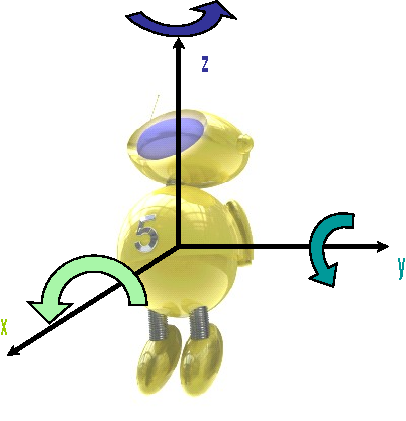
\includegraphics{img/reference-frame}
\end{center}

\begin{description}
\item[Origin] the center of mass of the robot
\item[X axis] oriented towards the front of the robot. If there is a
  camera, the front is defined by the default direction of the camera,
  otherwise the front will be seen as the natural frontal orientation
  for a mobile robot (the direction of ``forward'' movement). If the
  robot is not naturally oriented, the X axis will be chosen to match
  the main axis of symmetry of the robot body and it will be oriented
  towards the smallest side, typically the top of a cone for
  example. In case of a perfectly symmetrical body, the X axis can be
  chosen arbitrarily but a clear mark should be made visible on the
  robot body to indicate it.
\item[Z axis] oriented in the opposite direction from the gravity. If
  there is no gravity or natural up/down orientation in the
  environment or normal operation mode of the robot, the Z axis should
  be chosen in the direction of the main axis of symmetry in the
  orthogonal plane defined by the X axis, oriented towards the
  smallest side. In case of a perfectly symmetrical plane, the Z axis
  can be chosen arbitrarily but a clear mark should be made visible on
  the robot body to indicate it.
\item[Y axis] oriented to make a right-handed coordinate system.
\end{description}


The axes are oriented in a counter-clockwise direction, as depicted in
the illustration above.

\section{Component naming}

Each component A, which is a sub-component of component B has a name, distinct
from the name of all the other components at the same level.
This name is a generic designation of what A represents, such as ``leg''
,``head'', or ``finger''.

Using the correct name for each component is a critical part of this standard.
No formal rule can be given to find this name for any possible robot
configuration. However, this document includes a table covering many different
possible cases. We recommend that robot manufacturers pick from this table
the name that fits the most the description of their component.

\section{Localization}
When two identical components A1 and A2, such as the two legs of an humanoid
robots, are present in the same sub-component B, an extra node is inserted in
the hierarchy to differentiate them. This node is of the \code{Localizer} type,
and provides a \code{[]} operator, taking a \code{Localization} argument, used
to access each of the identical sub-components.
The \usdk provides an implementation for the \code{Localizer} and
\code{Localization} classes.
When possible, localization should be simple geometrical qualifier like
\textit{right}/\textit{center}/\textit{left},
\textit{front}/\textit{middle}/\textit{back} or
\textit{up}/\textit{in-between}/\textit{down}.
Note that ``right'' or ``front'' are
understood here from the point of view of a man standing and looking
in the direction of the X-axis of the robot, and \textit{up/pown}
matches the Z-axis, as depicted in the figure below:

\begin{center}
  
\includegraphics[width=.5\linewidth]{img/cube}
\end{center}

Several geometric qualifiers can be used at the same time to further
refine the position. In this case, multiple Localizer nodes are used.
As a convention, height information (U/I/D) comes first,
followed by depth information (F/M/H), and then side information (R/C/L).

\begin{urbiunchecked}
// Front-left wheel of a four-wheeled robot:
robot.body.wheel[front][left];
// Front laser of a robot equipped with multiple sonars:
robot.body.laser[front];
// Left camera from a robot with a stereo camera at the end of an arm:
robot.body.arm.camera[left];
// Top-left LED of the left eye.
robot.body.head.eye[left].led[up][left].val = 1;
// Touch sensor at the end of the front-left leg of a four-legged robot:
robot.body.leg[front][left].foot.touch;
\end{urbiunchecked}

You can further qualify a side+depth localization with an additional
F/B side information. This can be used in the typical layout below:

\begin{center}
  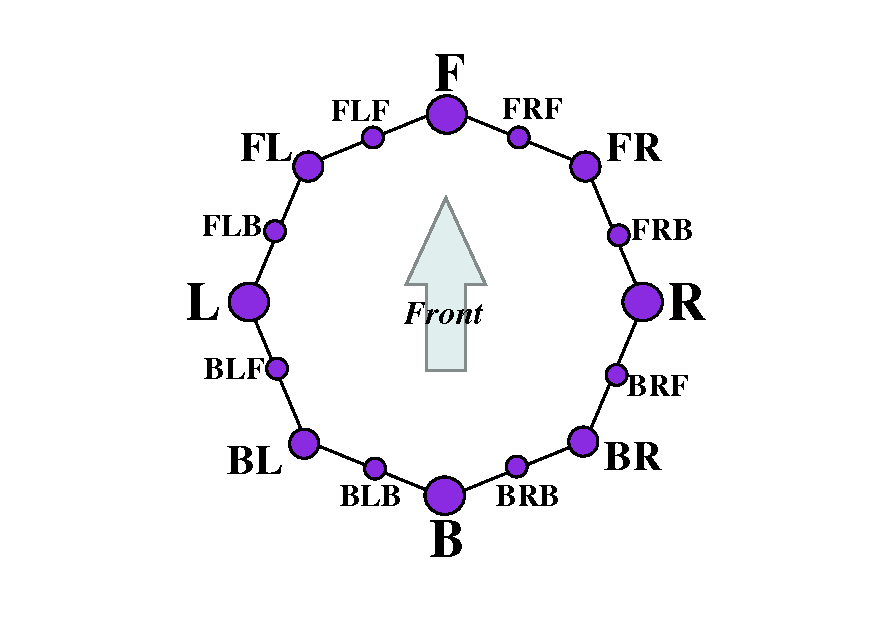
\includegraphics{img/localizer-multidim}
\end{center}

This dual positioning using side+depth can also be used to combine
side+height or height+depth information.

Layouts with a sequence of three or more identical components can use numbers
as their Localization, starting from 0.  The smaller the number, the closer to
the front, up, or left. For instance, an insectoid robot with 3 legs on each
side will use
\code{robot.body.leg[left][0]} to address the frontleft leg.

Layouts with identical components arranged in a circle can also use numeric
localization. The component with index 0 should be the uppermost, or front-most
if non applicable. Index should increase counterclockwise.

Some components like spines or tails are highly articulated with a set
of identical sub-components. When talking about these sub-components,
the above localization should be replaced by an array with a numbering
starting at 0. The smaller the number, the closer the sub-component is
to the robot main body. For surface-like sub-components, like skin
touch sensors, the array can be two dimensional.


Other possible localization for sensors are the X, Y and Z axis
themselves, like for example for an accelerometer or a gyro sensor,
available in each of the three directions.

\begin{urbiunchecked}
robot.body.accel[x]; // accelerometer in the x direction
\end{urbiunchecked}


Examples of component names including localization:

\begin{urbiunchecked}
leg[right], leg[left];
finger[right], finger[center], finger[left];      // three-finger hand
joint[0], joint[1] ... joint[5] // from tail
touch[478][124]                 // from skin
accel[x], accel[y], accel[z];         // typical accelerometer
gyro[x], gyro[y], gyro[z];            // typical gyro sensor
\end{urbiunchecked}

\section{Interface}
\label{sec:interface}

An ``interface'' describes some aspects of a type of device, by specifying the
slots and methods that implementations must provide. Each child node of
the component hierarchy should implement at least one interface.

For example, for a joint, we can have a ``Swivel'' interface, used to define
patella joints. For the robot body itself, we have a ``Mobile'' interface
describing mobile robots, which includes some standard way of
requesting a move forward, a turn, etc.

In short, interfaces are standard Urbi objects that components can inherit
from to declare that they have some functionalities.

The following pages describe a few of the most standard interfaces. Each
device in the component hierarchy which falls within the category of an
interface should implement it.

Each interface defines slots, which can be functions, events or plain data.
Some of those slots are optional: they are grayed and put around square
brackets in the following table.

\interface{Identity}

Contains information about the robot identity.

\begin{urbiscriptapi}
\item[type]%
  This describes the robot category among: humanoid, four-legged, wheeled,
  industrial arm. It gives a general idea of the robot family, but does not
  replace a more systematic probe of available services by investigating the
  list of attributes of the object.

\item[name]%
  Name of the robot.

\item[model] Model of the robot.

\item[serial] Serial number (if available).
\end{urbiscriptapi}


\interface{Network}

Contains information about the network identification of the robot.

\begin{urbiscriptapi}
\item[IP] IP address of the robot.
\end{urbiscriptapi}

\interface{Motor}

This interface is used to describe a generic motor controller.

\begin{urbiscriptapi}
\item[val] This slot is a generic pointer to a more specific slot describing
  the motor position, like \code{position} or \code{angle}, depending on the
  type of motor. It is mandatory in the Urbi Ready standard as a universal
  proxy to control an actuator. The more specific slot is described in a
  subclass of \code{Motor}.
\item[PGain?] Controls the P gain of the PID controller.
\item[IGain?] Controls the I gain of the PID controller.
\item[DGain?] Controls the D gain of the PID controller.
\end{urbiscriptapi}

\interface[Motor]{LinearMotor}


This interface is used to describe a linear motor controller.

A wheel can fall in this category, if the reported position is the distance
traveled by a point at the surface of the wheel.

\begin{urbiscriptapi}
\item[position] Position of the motor in meters.  Pointed to by the
  \code{val} slot.

\item[force] Intensity of the measured or estimated force applied on a
  linear motor.
\end{urbiscriptapi}

\interface[Motor]{LinearSpeedMotor}

Motor similar to \code{LinearMotor}, but controlled by its translation speed.

\begin{urbiscriptapi}
\item[speed] Translation speed in meters per second. Pointed to by the
  \code{val} slot.
\end{urbiscriptapi}


\interface[Motor]{RotationalMotor}


This interface is used to describe a position-controlled rotational motor
controller.

\begin{urbiscriptapi}
\item[angle] Angle of the motor in radian, modulo $2\pi$. Pointed to by the
  \code{val} slot.

\item[turn] Absolute angular position of the motor, expressed in number of
  turns.

\item[torque] Intensity of the measured or estimated torque applied on the
  motor.
\end{urbiscriptapi}

\interface[Motor]{RotationalSpeedMotor}

Interface describing a motor similar to \code{RotationalMotor} controlled
by its rotation speed.

\begin{urbiscriptapi}
\item[speed] Rotation speed in radians per second.
\end{urbiscriptapi}

\interface{Sensor}

This interface is used to describe a generic sensor.

\begin{urbiscriptapi}
\item[val] This slot is a generic pointer to a more specific slot describing
  the sensor value, like \code{distance} or \code{temperature}, depending on
  the type of sensor. It is mandatory in the Urbi Ready standard as a
  universal proxy to read a sensor. The more specific slot is described in a
  subclass of \code{Sensor}.
\end{urbiscriptapi}


\interface[Sensor]{DistanceSensor}

This interface is used to describe a distance sensor (infrared, laser,
ultrasonic...).

\begin{urbiscriptapi}
\item[distance] Measured distance expressed in meters.  Pointed to by the
  \code{val} slot.
\end{urbiscriptapi}


\interface[Sensor]{TouchSensor}

This interface is used to describe a touch pressure sensor (contact,
induction,...).

\begin{urbiscriptapi}
\item[pressure] Intensity of the pressure put on the touch sensor. Can be
  0/1 for simple buttons or expressed in Pascal units. Pointed to by the
  \code{val} slot.
\end{urbiscriptapi}


\interface[Sensor]{AccelerationSensor}

This interface is used to describe an accelerometer.

\begin{urbiscriptapi}
\item[acceleration] Acceleration expressed in $m/s^2$.  Pointed to by the
  \code{val} slot.
\end{urbiscriptapi}

\interface[Sensor]{GyroSensor}
This interface is used to describe an gyrometer.

\begin{urbiscriptapi}
\item[speed] Rotational speed in $\mathrm{rad}/s$.  Pointed to by the
  \code{val} slot.
\end{urbiscriptapi}

\interface[Sensor]{TemperatureSensor}
This interface is used to describe a temperature sensor.

\begin{urbiscriptapi}
\item[temperature] Measured temperature in Celsius degrees.  Pointed to by
  the \code{val} slot.
\end{urbiscriptapi}

\interface[Sensor]{Laser}
Interface for a scanning laser rangefinder, or other similar technologies.

\begin{urbiscriptapi}
\item[val] Last scan result. Can be either a list of ufloat, or a binary
  containing a packed array of doubles.

\item[angleMin] Start scan angle in radians, relative to the front of the
  device.

\item[angleMax] End scan angle in radians, relative to the front of the
  device.

\item[resolution] Angular resolution of the scan, in radians.

\item[distanceMin] Minimum measurable distance.

\item[distanceMax] Maximum measurable distance.

\item[rate?] Number of scans per second.
\end{urbiscriptapi}

Depending on the implementation, some of the parameters can be read-only, or
can only accept a few possible values. In that case it is up to the implementer
to select the closest possible value to what the user entered. It is the
responsibility of the user to read the parameter after setting it to check
what value will actually be used by the implementation.


\interface{Mobile}

Mobile robots all share this generic interface to provide high order
level motion control capabilities.

\begin{urbiscriptapi}
\item[go](<x>) Move approximately \var{x} meters forward if \var{x} is
  positive, backward otherwise.

\item[turn](<x>) Turn right approximately \var{x} radians.  \var{x} can be a
  positive or negative value.
\end{urbiscriptapi}

\interface{Tracker}

Camera-equipped robots can sometimes move the orientation of the field
of view horizontally and vertically, which is a very important feature
for many applications. In that case, this interface abstracts how such
motion can be achieved, whether it is done with a pan/tilt camera or
with whole body motion or a combination of both.

\begin{urbiscriptapi}
\item[yaw] Rotational articulation around the Z axis in the robot, expressed
  in radians.
\item[pitch] Rotational articulation around the Y axis in the robot,
  expressed in radians.
\end{urbiscriptapi}

\interface{VideoIn}

The VideoIn interface groups every information relative to cameras or any
image sensor.

\begin{urbiscriptapi}
\item[val] Image represented as a \code{Binary} value.
\item[xfov] The x field of view of the camera expressed in radians.
\item[yfov] The y field of view of the camera expressed in radians.

\item[height] Height of the image in the current resolution, expressed in
  pixels.

\item[width] Width of the image in the current resolution, expressed in
  pixels

\item[format?]
    Format of the image, expressed as an integer in the enum
    urbi::UImageFormat.  See below for more information.

\item[exposure?] Exposure duration, expressed in seconds. 0 if non
  applicable.

\item[wb?]  White balance (expressed with an integer value depending on the
  camera documentation). 0 if non applicable.

\item[gain?]  Camera gain amplification (expressed as a coefficient between
  0 and infinity). 1 if non applicable.

\item[resolution?]  Image resolution, expressed as an integer. 0 corresponds
  to the maximal resolution of the camera. Successive values correspond to
  all the supported image sizes in decreasing order.  Once modified, the
  effective resolution in X/Y can be checked with the width and height
  slots.

\item[quality?]  If the image is in the jpeg format, this slot sets the
  compression quality, from 0 (best compression, worst quality) to 100 (best
  quality, bigger image).
\end{urbiscriptapi}

The image sensor is expected to use the cheapest way in term of CPU and/or
energy consumption to produce images of the requested format.
Implementations linked to a physical image sensor do not have to implement
all the possible formats. In this case, the format closest to what was
requested must be used.
A generic image conversion object will be provided. In order to avoid
duplicate image conversions when multiple unrelated behaviors need the same
format, it is recommended that this object be instantiated in a slot of the
VideoIn object named after the format it converts to:
\begin{urbiunchecked}
if (!robot.body.head.camera.hasSlot("jpeg"))
{
  var robot.body.head.camera.jpeg =
    ImageConversion.new(robot.body.head.camera.getSlot("val"));
  robot.body.head.camera.jpeg.format = 3;
}
\end{urbiunchecked}

\interface{AudioOut}
The AudioOut interface groups every information relative to speakers.

\begin{urbiscriptapi}
\item[val] The speaker value, expressed as a binary, in the format given by
  the binary header during the assignment.

  Speakers are write-only devices, so there is not much sense in reading the
  content of this attribute. At best, it returns the remaining sound to be
  played if it is not over yet, but this is not a requirement.


\item[remain] The amount of time remaining to play in the speaker sound
  buffer (expressed in \textit{ms} as a default unit).


\item[playing] This is a Boolean value which is true when there is a sound
  currently playing (the buffer is not empty)%

\item[volume?] Volume of the play back, in decibels.
\end{urbiscriptapi}



\interface{AudioIn}

The AudioIn interface groups every information relative to microphones.

\begin{urbiscriptapi}
\item[val] Binary value corresponding to the sound heard, expressed in the
  current unit (wav, mp3...). The unit can be changed like any other regular
  unit in Urbi.

  The content is the sound heard by the microphone since the last update
  event.
\item[duration] Amount of sound in the val attribute, expressed in
  \textit{ms}.
\item[gain?] Microphone gain amplification (expressed between 0 and 1).
\end{urbiscriptapi}


\interface{BlobDetector}

Ball detectors, marker detectors and various feature-based detectors
should all share a similar interface. They extract a part of the image
that fits some criteria and define a \dfn{blob} accordingly. Here are
the typical slots expected:

\begin{urbiscriptapi}
\item[x] The x position of the center of the blob in the image

\item[y] The y position of the center of the blob in the image

\item[ratio] The size of the blob expressed as a normalized image size: 1 =
  full image, 0 = nothing.

\item[visible] A Boolean expressing whether there is a blob in the image or
  not (see \refSlot{threshold}).

\item[threshold] The minimum value of ratio to decide that the blob is
  visible.

\item[orientation?]  Angle of the main ellipsoid axis of the blob (0 =
  horizontal), expressed in radians.

\item[elongation?]  Ratio between the main and the second diameter of the
  blob enveloping ellipse.
\end{urbiscriptapi}

\interface{TextToSpeech}
Text to speech allows to read text using a speech synthesizer. Default
implementations should use the \code{speaker} component (or alias) as
their default sound output.

\begin{urbiscriptapi}
\item[lang?]  The language used, in international notation (fr, en, it…):
  ISO 639

\item[speed?]  How fast the voice should go.  A positive number, with 1
  standing for ``regular speed''.

\item[pitch?] Voice pitch.  A positive number, with 1 standing the regular
  pitch.

\item[gender?] Gender of the speaker (0:male/1:female).

\item[age?] Age of the speaker, if applicable.

\item[voice?]
    Most TTS engines propose several voices, this attribute allows picking
    one. It's a string identifier specific to the TTS developer.

\item[say](s) Speak the sentence given in parameter \var{s}.

\item[voicexml?](s) Speak the text \var{s} expressed as a VoiceXML string.

\item[script?](s) Speak the text \var{s} augmented by script markups (see
  specific Gostai documentation) to generate \urbi events.
\end{urbiscriptapi}


\interface{SpeechRecognizer}

Speech recognition allows to transform a stream of sound into a text
using various speech recognition algorithms. Implementations
should use the \code{micro} component as their default sound input.

\begin{urbiscriptapi}
\item[lang?]  The language used, in international notation (fr, en, it…):
  ISO 639.
\item[hear](s) This event has one parameter which is the string describing
  what the speech engine has recognized (can be a word or a sentence).
\end{urbiscriptapi}

\interface{Led}

Simple uni-color Led.

\begin{urbiscriptapi}
\item[val] Led intensity between 0 and 1.
\end{urbiscriptapi}


\interface[Led]{RGBLed}

Tri-color led.

\begin{urbiscriptapi}
\item[r] Intensity of the red component, between 0 and 1.
\item[g] Intensity of the green component, between 0 and 1.
\item[b] Intensity of the blue component, between 0 and 1.
\end{urbiscriptapi}

\interface{Battery}

Power source of any kind.

\begin{urbiscriptapi}
\item[remain] Estimation of the remaining energy between 0 and 1.
\item[capacity] Storage capacity in Amp.Hour.
\item[current] Current current consumption in Amp.
\item[voltage] Current voltage in Volt.
\end{urbiscriptapi}


\section{Standard Components}

Standard components correspond to components typically found in wheeled
robots, humanoid or animaloid robots, or in industrial arms. This section
provides a list of such components. Whenever possible, robots compatible with
the \gsrapi should name all the components in the hierarchy using this list.

\subsection{Yaw/Pitch/Roll orientation}
\label{sec:naming:ypr}

Note that \gsrapi considers the orientation to be a component name, and
not a localizer. So one would write \lstinline|head.yaw| and not
\lstinline|head.joint[yaw]| to refer to a rotational articulation of the head
around the Z axis.

It is not always clear which rotational direction corresponds to the
yaw, pitch or roll components (listed in the table below). This is a
quick guideline to help determine the proper association.

Let us consider the robot in its resting, most prototypical position,
like ``standing'' on two or four legs for a humanoid or animaloid, and
let all members ``naturally'' fall under gravity. When gravity has no
effect on a certain joint (because it is in the orthogonal plan to Z,
for example), the medium position between rangemin and rangemax should
be used. The body position achieved will be considered as a reference.
Then for each component that is described in terms of yaw/pitch/roll
sub-decomposition, the association will be as follow:

\begin{description}
\item[yaw] rotational articulation around the Z axis in the robot.
\item[pitch] rotational articulation around the Y axis in the robot.
\item[roll] rotational articulation around the X axis in the robot.
\end{description}

When there is no exact match with the X/Y/Z axis, the closest match, or
the default remaining available axis, should be selected to determine
the yaw/pitch/roll meaning.

\subsection{Standard Component List}
\label{sec:naming:components}

The following table summarizes the currently referenced standard
components, with a description of potential components that they could
be sub-component of, a description of potential components they may
contain, and a list of relevant interfaces. This table should be seen as a
quick reference guide to identify available components in a given
robot.

\newcommand{\component}[5]
{
  \lstindex{#1} &
  #5 &
  \code{#2} &
  \code{#3} &
  \code{#4}\\\hline
}

\tablehead{\hline
\textbf{Name} &
\textbf{Description} &
\textbf{Sub. of} &
\textbf{Contains} &
\textbf{Facets} \\\hline}
\begin{supertabular}{|m{.115\linewidth}|m{.45\linewidth}|*{4}{m{.12\linewidth}|}}
  \component{robot}{}{body}{Identity Network Mobile Tracker}{
    %%
    This is the main component that represents an abstraction of the
    robot, and the root node of the whole component hierarchy.
    %%
  }

  \component{body}{robot}{wheel arm leg neck head wheel tail skin torso
    \ldots}{}{
    %%
    This is the main component that contains every piece of hardware
    in the robot. This includes all primary kinematics sub-chains
    (arms, legs, neck, head, etc) and non-localized sensor arrays,
    typically body skin or heat detectors.  Localized sensors, like
    fingertips touch sensors, will typically be found attached to the
    finger component they belong and not directly to the body.
    %%
  }

  \component{wheel}{body}{}{Rotational\-Motor}{
    %%
    Wheel attached to its parent component.
    %%
  }
  \component{leg}{body}{hip knee ankle foot joint}{}{
    %%
    Legs are found in humanoid or animaloid robots and correspond to
    part of the kinematics chain that are attached to the main body by
    one extremity only and which do touch the ground in normal
    operation mode (unlike arms). A typical configuration for
    humanoids contains a hip, a knee and an ankle. If the leg is more
    segmented, the leg can be described with a simple array of joints.
    %%
  }

  \component{arm}{body}{shoulder elbow wrist hand grip joint}{}{
    %%
    Unlike legs, an arm's extremity does not always touch the ground
    in normal operating mode. This applies to humanoid robots or
    single-arm industrial robots. Arms supersede legs in the
    nomenclature: if a body part behaves alternatively like an arm and
    like a leg, it will be considered as an arm.
    %%
  }

  \component{shoulder}{arm}{yaw pitch roll}{}{
    %%
    The shoulder is the upper part of the arm. It can have one, two or
    three degrees of freedom and is the closest part of the arm
    relative to the body.
    %%
  }

  \component{elbow}{arm}{pitch}{}{
    %%
    Separates the upper arm and the lower arm, this is usually a
    single rotational axis.
    %%
  }

  \component{wrist}{arm}{yaw pitch roll}{}{
    %%
    Connects the hand and the lower part of the arm. Usually three
    degrees of freedom axis.
    %%
  }

  \component{hand}{arm}{finger}{}{
    %%
    The hand is an extension of the arm that usually holds
    fingers. It's not the wrist, which is articulated and between the
    arm and the hand.
    %%
  }

  \component{finger}{hand}{touch}{Motor}{
    %%
    Fingers are a series of articulated motors at the extremity of the
    arm, and connected to the hand. They are usually localized with
    arrays and/or lateral localization respective to the hand.
    %%
  }

  \component{grip}{arm hand}{touch}{Motor}{
    %%
    Simple two-fingers system.
    %%
  }

  \component{hip}{leg}{yaw pitch roll}{}{
    %%
    The hip is the upper part of the leg and connects it to the main
    body. It can have one, two or three degrees of freedom.
    %%
  }

  \component{knee}{leg}{pitch}{}{
    %%
    Separates the upper leg and the lower leg, this is usually a
    single rotational axis.
    %%
    }

  \component{ankle}{leg}{yaw pitch roll}{}{
    %%
    Connects the foot and the lower part of the leg. Usually three
    degrees of freedom axis.
    %%
    }

  \component{foot}{leg}{touch}{}{
    %%
    The foot is an extension of the leg that usually holds toes. It's
    not the ankle, which is articulated and between the leg and the
    foot. The foot can also contain touch sensors in simple
    configurations.
    %%
  }

  \component{toe}{foot}{touch}{Motor}{
    %%
    Like fingers, but attached to the foot.
    %%
  }

  \component{neck}{body}{yaw pitch roll}{}{
    %%
    The neck corresponds to a degree of freedom not part of the head,
    but relative to the rigid connection between the head and the main
    body.
    %%
  }

  \component{tail}{body}{joint}{}{
    %%
    A tail is a series of articulated motors at the back of the robot.
    %%
  }

  \component{head}{body neck}{camera mouth ear lip eye eyebrow}{}{
    %%
    The head main pivotal axis.
    %%
  }

  \component{mouth}{head}{lip}{Motor}{
    %%
    The robot mouth (open/close)
    %%
  }

  \component{ear}{head}{}{Motor}{
    %%
    Ears may have degrees of freedom in certain robots.
    %%
  }

  \component{joint}{tail arm leg lip}{}{Motor}{
    %%
    Generic articulation in the robot.
    %%
  }

  \component{yaw}{body neck knee ankle shoulder elbow wrist
    torso}{}{Rotational\-Motor Rotational\-Speed\-Motor}{
    %%
    Rotational articulation around the Z axis in the
    robot. See \autoref{sec:naming:ypr}.
    %%
  }

  \component{pitch}{body neck knee ankle shoulder elbow wrist
    torso}{}{Rotational\-Motor Rotational\-Speed\-Motor}{
    %%
    Rotational articulation around the Y axis in the
    robot.  See \autoref{sec:naming:ypr}.
    %%
  }

  \component{roll}{body neck knee ankle shoulder elbow wrist
    torso}{}{Rotational\-Motor Rotational\-Speed\-Motor}{
    %%
    Rotational articulation around the X axis in the robot. See
    \autoref{sec:naming:ypr}.
    %%
  }

  \component{x}{body arm}{}{Linear\-Motor Linear\-Speed\-Motor}{
    %%
    Translational movement along the X axis.
    %%
  }

  \component{y}{body arm}{}{Linear\-Motor Linear\-Speed\-Motor}{
    %%
    Translational movement along the Y axis.
    %%
  }

  \component{z}{body arm}{}{Linear\-Motor Linear\-Speed\-Motor}{
    %%
    Translational movement along the Z axis.
    %%
  }

  \component{lip}{mouth}{joint}{Motor}{
    %%
    Corresponds to animated lips.
    %%
  }

  \component{eye}{head}{camera}{}{
    %%
    Corresponds to the eyeball pivotal axis.
    %%
    }

  \component{eyebrow}{head}{joint}{Motor}{
    %%
    Some robots will have eyebrows with generally one or several
    degrees of freedom.
    %%
    }

  \component{torso}{body}{yaw pitch roll}{}{
    %%
    This corresponds to a pivotal or rotational axis in the middle of
    the main body.
    %%
    }

  \component{spine}{torso}{joint}{}{
    %%
    This is a more elaborated version of ``torso'', with a series of
    articulations to give several degrees of freedom in the back of
    the robot.
    %%
    }

  \component{clavicle}{body}{}{Motor}{
    %%
    This is not to be mixed up with the ``top of the arm'' body part. It
    is an independent degree of freedom that can be used to bring the
    two arms closer in a sort of ``shoulder raising'' movement.
    %%
    }

  \component{touch}{finger grip foot toe}{}{TouchSensor}{
    %%
      Touch sensor.
    %%
    }

  \component{gyro}{body}{}{GyroSensor}{
    %%
      Gyrometer sensor.
    %%
    }

  \component{accel}{body}{}{Accel\-eration\-Sensor}{
    %%
      Accelerometer sensor.
    %%
    }

  \component{camera}{head body}{}{VideoIn}{
    %%
    Camera sensor. If several cameras are available, localization
    shall apply; however there must always be an alias from
    \code{camera} to one of the effective cameras (like \code{cameraR}
    or \code{cameraL}).
    %%
    }

  \component{speaker}{head body}{}{AudioIn}{
    %%
    Speaker device. If several speakers are available, localization
    shall apply; however there must always be an alias from
    \code{speaker} to one of the effective speakers (like
    \code{speakerR} or \code{speakerL}).
    %%
    }

  \component{micro}{head body}{}{AudioOut}{
    %%
    Microphone devices. If several microphones are available,
    localization shall apply; however there must always be an alias
    from \code{micro} to one of the effective microphones (like
    \code{microR} or \code{microL}).
    %%
  }

  \component{speech}{robot}{}{Speech\-Recognizer}{
    %%
      Speech recognition component.
    %%
    }

  \component{voice}{robot}{}{TextTo\-Speech}{
    %%
      Voice synthesis component.
    %%
    }

\end{supertabular}



\section{Compact notation}

Components are usually identified with their full-length name, which is
the path to access them inside the structure tree. For convenience and
backward compatibility with pre-2.0 versions of \urbi, there is also a
compact notation available. We will describe here how to construct the
compact notation starting from the full name and the structure tree.

\tablehead{\hline
Full name &
Compact name\\\hline}
\begin{supertabular}{|m{9.008cm}|m{5.533cm}|}
\code{robot.body.armR.elbow} &
\code{elbowR} \\\hline
\code{robot.body.head.yaw} &
\code{headYaw} \\\hline
\code{robot.body.legL.knee.pitch} &
\code{kneeL} \\\hline
\code{robot.body.armR.hand.finger[3][2]} &
\code{fingerR[3][2]} \\\hline
\code{robot.body.armL.hand.fingerR} &
\code{fingerLR} \\\hline
\end{supertabular}

The rule is to move every localization qualifier at the end of the
compact notation, in the order where they appear in the full-length
name. The remaining component names should then be considered one by
one to see if they are needed to remove ambiguities. If they are not,
like typically the robot or body components which are shared with
almost every other full-length name, they can be ignored. If finally
several component names have to be kept, they should be separated by
using upper case letters for the first character instead of a dot, like
in Java-style notation.

\begin{example}[\code{robot.body.armL.hand.fingerR}]~\\
  \begin{enumerate}
  \item Move all localization at the end:
    \code{robot.body.arm.hand.fingerLR}
  \item The full name remaining is: \code{robot.body.arm.hand.finger}
  \item \code{finger} should be kept, \code{hand}, \code{arm},
    \code{body} and \code{robot} are not necessary since every
    finger component will always be attached only to a hand, itself
    attached to an arm and a body and a robot.
  \item The result is \code{fingerLR}
  \end{enumerate}
\end{example}


\begin{example}[\code{robot.body.head.yaw}]~\\
  \begin{enumerate}
  \item No localization to move
  \item \code{yaw} must be kept because \code{head} also have a
    \code{pitch} sub-component and
  \item \code{head} must also be kept to avoid ambiguity with other
    components having a \code{yaw} sub-component.
  \item The result is \code{headYaw}
  \end{enumerate}
\end{example}

\begin{example}[\code{robot.body.legL.knee.pitch}]~\\
  \begin{enumerate}
  \item Move all localization at the end:
    \code{robot.body.leg.knee.pitchL}
  \item \code{pitch} is not necessary because \code{knee} has only a
    \code{pitch}, so \code{knee} will be kept only
  \item The result is \code{kneeL}
  \end{enumerate}
\end{example}

\section{Support classes}
The \usdk provides a few support \us classes to help you build the component
hierarchy.  You can access to those classes by including the files
\file{urbi/naming-standard.u} and \file{urbi/component.h}.

\let\subsectionOrig\subsection
\let\subsection\subsectionObject

\subsection{Interface}

The \code{Interface} class contains \us objects for all the interfaces defined
in this document. Implementations must inherit from the correct interface.

\begin{urbiunchecked}
// Instantiate a camera.
var cam = myCamera.new();
// Make it inherit from VideoIn.
cam.addProto(Interface.VideoIn);
\end{urbiunchecked}

The \code{Interface.interfaces} method can be called to get a list of all
the interfaces an object implements.

\subsection{Component}

The \code{Component} class can be used to create intermediate nodes of the
hierarchy. It provides the following methods:

\begin{urbiscriptapi}

\item[addComponent](<name>)%
  Add a new sub-component to the current component. \var{name} can
  be the name of the new component to create, or an instance of
  \code{Component}.

\item[addDevice](<name>, <value>)%
  Add device \var{value} as sub-component, under the name \var{name}. The
  device must inherit from at least one Interface.

\item[makeCompactNames]%
  This function must be called once on the root node (\code{robot})
  after the hierarchy is completed.  It automatically computes the
  short name of all the devices, and insert them as slots of the
  \code{Global} object.

\item[dump]%
  Display a hierarchical view of the component hierarchy.

\item[flatDump]%
  Display all the devices in the hierarchy, sorted by the Interface
  they implement.
\end{urbiscriptapi}

\subsection{Localizer}

The \code{Localizer} class is a special type of \code{Component} that stores
other components based on their localization. It provides a \code{[]} operator
that takes a \code{Localization}, such as \lstinline|top,left,front|, and that
can be used to set and get the \code{Component} or device associated with
that \code{Localization}.

Note that the \code{[]} function is using a mechanisms to automatically look
for its argument as a slot of \code{Localizer}. As a consequence, you cannot
pass a variable to this function, but only one of the constant
\code{Localization}.
To pass a variable, use the \code{get(loc)} or the \code{set(loc, value)}
function.

The following example illustrates a typical instantiation sequence:

\begin{urbiunchecked}
// Create the top-level node.
var Global.robot = Component.new("robot");
robot.addComponent("head");
var cam = MyCamera.new;
cam.addProto(Interface.VideoIn);
robot.head.addDevice("camera", cam);
// Add two wheels
robot.addComponent(Localizer.new("wheel"));
robot.wheel[left] = MyWheel.new(0).addProto(Interface.RotationalMotor);
robot.wheel[right] = MyWheel.new(1).addProto(Interface.RotationalMotor);
// Implement the Mobile facet in urbiscript:
var robot.go = function(d)
{
  robot.wheel.val = robot.wheel.val + d / wheelRadius adaptive:1
};
var robot.turn = function(r)
{
  var v = r * wheelDistance / wheelRadius;
  robot.wheel[left].val = robot.wheel[left].val + v adaptive:1 &
  robot.wheel[right].val = robot.wheel[right].val - v adaptive:1
};
robot.addProto(Interface.Mobile);
robot.makeCompactNames;
// Let us see the result:
robot.flatDump;
[00010130] *** Mobile: robot
[00010130] *** RotationalMotor: wheelL wheelR
[00010130] *** VideoIn: camera
\end{urbiunchecked}

%% Restore the definition of \section.
\let\subsection\subsectionOrig

%%% Local Variables:
%%% mode: latex
%%% TeX-master: "../urbi-sdk"
%%% ispell-dictionary: "american"
%%% ispell-personal-dictionary: "../urbi.dict"
%%% fill-column: 76
%%% End:


%%% Local Variables:
%%% mode: latex
%%% TeX-master: "../urbi-sdk"
%%% ispell-dictionary: "american"
%%% ispell-personal-dictionary: "../urbi.dict"
%%% fill-column: 76
%%% End:

\ifthen{\boolean{platforms}}
{
  %% Copyright (C) 2009-2010, Gostai S.A.S.
%%
%% This software is provided "as is" without warranty of any kind,
%% either expressed or implied, including but not limited to the
%% implied warranties of fitness for a particular purpose.
%%
%% See the LICENSE file for more information.

\part{\urbi Platforms}
\label{part:platforms}

%% Copyright (C) 2010, Gostai S.A.S.
%%
%% This software is provided "as is" without warranty of any kind,
%% either expressed or implied, including but not limited to the
%% implied warranties of fitness for a particular purpose.
%%
%% See the LICENSE file for more information.

\begin{partDescription}{part:specs}
  {
    %
    This part defines the specifications of the \us language version
    2.0. It defines the expected behavior from the \us interpreter,
    the standard library, and the \sdk. It can be used to check
    whether some code is valid, or browse \us or \Cxx \api for a
    desired feature. Random reading can also provide you with advanced
    knowledge or subtleties about some \us aspects.

    This part is not an \us tutorial; it is not structured in a
    progressive manner and is too detailed.  Think of it as a
    dictionary: one does not learn a foreign language by reading a
    dictionary. The \us Tutorial (\autoref{part:tut}), or the live \us
    tutorial built in the interpreter are good introductions to \us.

    This part does not aim at giving advanced programming
    techniques. Its only goal is to define the language and its
    libraries.
    %
  }
\item[sec:tools]
  Presentation and usage of the different tools available with the
  \urbi framework related to \us, such as the \urbi server, the
  command line client, \umake, \ldots

\item[sec:lang]
  Core constructs of the language and their behavior.

\item[sec:stdlib]
  Listing of all classes and methods provided in the standard library.

\item[sec:specs:ros] \urbi provides a set of tools to communicate with ROS
  (Robot Operating System). For more information about ROS, see
  \url{http://www.ros.org}.  \urbi, acting as a ROS node, is able to
  interact with the ROS world.

\item[sec:naming]
  Also known as ``The \urbi Naming Standard'': naming conventions in
  for standard hardware/software devices and components implemented as
  UObject and the corresponding slots/events to access them.

%\item[sec:sdk]
%  The \urbi software development kit that enable to
%  interact with \urbi from \Cxx.
\end{partDescription}


%%% Local Variables:
%%% mode: latex
%%% TeX-master: "../urbi-sdk"
%%% ispell-dictionary: "american"
%%% ispell-personal-dictionary: "../urbi.dict"
%%% fill-column: 76
%%% End:


%% Alphabetical.
\newcommand{\inputPlatform}[1]{%
  \ifthen{\boolean{#1}}{\input{platforms/#1}}
}

\inputPlatform{bioloid}
\inputPlatform{nxt}
\inputPlatform{nao}
\inputPlatform{p3dx}
\inputPlatform{rmp}
\inputPlatform{spykee}
\inputPlatform{webots}

%%% Local Variables:
%%% mode: latex
%%% TeX-master: "../urbi-sdk"
%%% ispell-dictionary: "american"
%%% ispell-personal-dictionary: "../urbi.dict"
%%% fill-column: 76
%%% End:

}
%% Copyright (C) 2010, Gostai S.A.S.
%%
%% This software is provided "as is" without warranty of any kind,
%% either expressed or implied, including but not limited to the
%% implied warranties of fitness for a particular purpose.
%%
%% See the LICENSE file for more information.

\part{Tables and Indexes}
\label{part:tables}

%% Copyright (C) 2010, Gostai S.A.S.
%%
%% This software is provided "as is" without warranty of any kind,
%% either expressed or implied, including but not limited to the
%% implied warranties of fitness for a particular purpose.
%%
%% See the LICENSE file for more information.

\begin{partDescription}{part:specs}
  {
    %
    This part defines the specifications of the \us language version
    2.0. It defines the expected behavior from the \us interpreter,
    the standard library, and the \sdk. It can be used to check
    whether some code is valid, or browse \us or \Cxx \api for a
    desired feature. Random reading can also provide you with advanced
    knowledge or subtleties about some \us aspects.

    This part is not an \us tutorial; it is not structured in a
    progressive manner and is too detailed.  Think of it as a
    dictionary: one does not learn a foreign language by reading a
    dictionary. The \us Tutorial (\autoref{part:tut}), or the live \us
    tutorial built in the interpreter are good introductions to \us.

    This part does not aim at giving advanced programming
    techniques. Its only goal is to define the language and its
    libraries.
    %
  }
\item[sec:tools]
  Presentation and usage of the different tools available with the
  \urbi framework related to \us, such as the \urbi server, the
  command line client, \umake, \ldots

\item[sec:lang]
  Core constructs of the language and their behavior.

\item[sec:stdlib]
  Listing of all classes and methods provided in the standard library.

\item[sec:specs:ros] \urbi provides a set of tools to communicate with ROS
  (Robot Operating System). For more information about ROS, see
  \url{http://www.ros.org}.  \urbi, acting as a ROS node, is able to
  interact with the ROS world.

\item[sec:naming]
  Also known as ``The \urbi Naming Standard'': naming conventions in
  for standard hardware/software devices and components implemented as
  UObject and the corresponding slots/events to access them.

%\item[sec:sdk]
%  The \urbi software development kit that enable to
%  interact with \urbi from \Cxx.
\end{partDescription}


%%% Local Variables:
%%% mode: latex
%%% TeX-master: "../urbi-sdk"
%%% ispell-dictionary: "american"
%%% ispell-personal-dictionary: "../urbi.dict"
%%% fill-column: 76
%%% End:


%% Copyright (C) 2010, Gostai S.A.S.
%%
%% This software is provided "as is" without warranty of any kind,
%% either expressed or implied, including but not limited to the
%% implied warranties of fitness for a particular purpose.
%%
%% See the LICENSE file for more information.

\chapter{Notations}
\label{sec:notations}

This chapter introduces the various notations that are used in the
document.

\section{Words}

\begin{itemize}
\item \var{name}\\
  Depending on the context, a \dfn{variable} name (i.e., an identifier
  in \Cxx or \us), or a \dfn{meta-variable} name.  A meta-variable
  denotes a place where some syntactic construct may be entered.  For
  instance, in \lstinline|while (\var{expression}) \var{statement}|,
  \var{expression} and \var{statement} do not denote two variable
  names, but two placeholders which can be filled with an arbitrary
  expression, and an arbitrary statement.  For instance:

  \lstinline|while (!tasks.empty) { tasks.removeFront.process }|.

\item \env{name}\\
  An environment variable name, e.g., \env{PATH}.
\item \lstinline|code|\\
  A piece of \us or \Cxx code.
\item \file{name}\\
  A file name.
\end{itemize}

\section{Frames}

\subsection{Shell Sessions}
\label{sec:notations:shell}

Interactive sessions with a (Unix) shell are represented as follows.

\begin{shell}
$ echo toto
toto
\end{shell}

The user entered \samp{echo toto}, and the system answered
\samp{toto}.  \samp{\$} is the \dfn{prompt}: it starts the lines where
the system invites the user to enter her commands.

\subsection{\us Sessions}

Interactive sessions with \urbi are represented as follows.

\begin{urbiscript}[firstnumber=1]
echo("toto");
[00000001] *** toto
\end{urbiscript}

Contrary to shell interaction (see \autoref{sec:notations:shell}),
there is no prompt that marks the user-entered lines (here
\lstinline|echo("toto");|, but, on the contrary, answers from the \urbi
server start with a label that includes a timestamp (here
\samp{00000001}), and possibly a channel name, \samp{output} in the
following example.

\begin{urbiscript}
cout << "toto";
[00000002:output] "toto"
\end{urbiscript}


\subsection{\us Assertions}

\us features assertions blocks, see \autoref{sec:assertions}.  The
following assertion frame:

\begin{urbiassert}
1 == 2 / 2;
1 < 2;
true;
"foobar"[0, 3] == "foo";
[1, 2, 3].map (function (a) { a * a }) == [1, 4, 9];
[ => ].empty;
\end{urbiassert}

\noindent
actually denotes the following assertion-block in an \us-session
frame:

\begin{urbiscript}
assert
{
  true;
  1 < 2;
  1 + 2 * 3 == 7;
  "foobar"[0, 3] == "foo";
  [1, 2, 3].map (function (a) { a * a }) == [1, 4, 9];
  [ => ].empty;
};
\end{urbiscript}

\subsection{\Cxx Code}

\Cxx source code is presented in frames as follows.

\begin{cxx}
class Int
{
public:
  Foo(int v = 0)
    : val_(v)
  {}

  void operator(int v)
  {
    std::swap(v, val_);
    return v;
  }

  int operator() const
  {
    return val_;
  }

private:
  int val_;
};
\end{cxx}

%%% Local Variables:
%%% mode: latex
%%% TeX-master: "urbi-sdk"
%%% ispell-dictionary: "american"
%%% ispell-personal-dictionary: "urbi.dict"
%%% fill-column: 76
%%% End:

%% Copyright (C) 2010, Gostai S.A.S.
%%
%% This software is provided "as is" without warranty of any kind,
%% either expressed or implied, including but not limited to the
%% implied warranties of fitness for a particular purpose.
%%
%% See the LICENSE file for more information.

\chapter{Release Notes}
\label{sec:news}

This chapter lists the user-visible changes in \usdk releases.

\section{\usdk 2.3}
Released on 2010-09-28.

\subsection{Fixes}
\begin{itemize}
\item \refSlot[Date]{asFloat} is restored.
\item \refSlot[File]{create} empties existing files first.
\item \refSlot[Lobby]{lobby} always returns the current lobby, even if
  invoked on another lobby.
\item \refSlot[Object]{inspect} works properly, even if the target is a
  remote lobby.
\item \slot[Regexp]{match}s renamed as \refSlot[Regexp]{matches}.
\item \refSlot[System]{version} Really returns the current version.
\item Fix multiple race conditions in RTP handling code preventing proper
  initialization of remote UObjects.
\item Fix Windows deployment to have both debug and release UObjects
  installed.
\item Fix \command{urbi-sound} in the liburbi examples.
\item Fix server mode of \samp{urbi-launch --remote}.
\end{itemize}

\subsection{New Features}
\begin{itemize}
\item The documentation of \urbi SDK Remote, our middleware layer to
  communicate with an \urbi server --- either by hand or via the UObjects
  ---, is included in the binary packages (in
  \file{share/doc/urbi-sdk/sdk-remote.htmldir/index.html}.  It is also
  available on-line at
  \url{\downloadUrl/\packageTarname/\packageVersion/doc/sdk-remote.htmldir}.

\item In addition to Gostai Console 2.5, Windows installers of \usdk now
  include the Gostai Editor 2.4.1.

\item By popular demand, all the Boost libraries (1.38) are included in the
  binary packages.  We used to provide only the headers and libraries \usdk
  depends upon.  Boost.Python, because it has too many dependencies, is not
  included.

\item When launched with no input (i.e., none of the options
  \option{-e}/\option{--expression}, \option{-f}/\option{--file},
  \option{-P}/\option{--port} were given), the interpreter is interactive.

\item Assignment operators such as \lstinline|'+='| are redefinable.  See
  \autoref{sec:lang:iass}.

\item \refSlot[Date]{'-'} accepts a \refObject{Duration} or a
  \refObject{Float} in addition to accepting a \refObject{Date}.

\item \refSlot[Float]{fresh} generates unique integers.

\item \refSlot[InputStream]{close}.

\item \refSlot[List]{'+='}.

\item Support for \lstinline|else| in \lstinline|try| blocks
  (\autoref{sec:lang:catch}).  Run only when the \lstinline|try|
  block completed properly.
\begin{urbiscript}
// Can we run "riskyFeature"?
try { riskyFeature } catch { false } else { true };
[00004220] false

function riskyFeature() { throw "die" }|;
try { riskyFeature } catch { false } else { true };
[00004433] false

riskyFeature = function () { 42 }|;
try { riskyFeature } catch { false } else { true };
[00004447] true
\end{urbiscript}

\item Support for \lstinline|finally| in \lstinline|try| blocks
  (\autoref{sec:lang:except:finally}).  Use it for code that must be run
  whatever the control flow can be.  For instance:
\begin{urbiscript}
try { echo(1) } catch { echo(2) } else { echo(3) } finally { echo(4) };
[00002670] *** 1
[00002670] *** 3
[00002670] *** 4

try { throw 1 } catch { echo(2) } else { echo(3) } finally { echo(4) };
[00002671] *** 2
[00002671] *** 4
\end{urbiscript}

\item \refSlot[System]{eval} and \refSlot[System]{load} report syntax
  warnings.
\begin{urbiscript}
eval("new Object");
[00001388:warning] !!! 1.1-10: `new Obj(x)' is deprecated, use `Obj.new(x)'
[00001388:warning] !!!    called from: eval
[00001388] Object_0x1001b2320
\end{urbiscript}
\item New functions \lstinline|as| and \lstinline|fill| on UVar to ease access
to the generic cast system.
\item Add support to \code{boost::unordered\_map} to UObject casting system.
\item Optimize remote UObjects: notifies between two objects in the same
  process instance are transmitted locally.
\item Provide a \code{CustomUVar} class to ease encapsulation of custom data
  in UVar.
\item Bind the \code{constant} property on UVar.
\end{itemize}


\section{\usdk 2.2}
Released on 2010-08-23.

\subsection{Fixes}
\begin{itemize}
\item The main loop optimization triggered several issues with GNU/Linux and
  Mac OS X in interactive sessions (truncated output, possibly blocked
  input).  These issues are fixed on Snow Leopard and Leopard and GNU/Linux.
\item Deep overall of the event handling primitives.  Watching an expression
  will succeed in cases where it used to fail.  For instance:

\begin{urbiscript}
at (isdef (myVar))
  echo("var myVar = " + myVar),

myVar;
[00000001:error] !!! lookup failed: myVar

var myVar = 42|;
[00000003] *** var myVar = 42
\end{urbiscript}

\noindent
or

\begin{urbiunchecked}
var x = 0|;
function f() { x == 1 }|;
at (f()) echo("OK");
x = 1|;
[00000001] *** OK
\end{urbiunchecked}

  Support for sustained events is fixed too (see \autoref{sec:lang:at}).
\item \refSlot[List]{max} and \refSlot[List]{min} will now report the right
  indexes in error messages.
\item \lstinline|onleave| blocks on lasting events are now run
  asynchronously, as expected.
\item \lstinline|at (expression ~ duration)| is now supported.
\item Fix a bug if emitting an event triggers its unsubscription.
\item Fix printing of \lstinline|Exception.Type| and
  \lstinline|Exception.ArgumentType|.
\item Fix timestamp overflow on Windows after 40 minutes.
\item Fix fatal error when manipulating the first \var{Job} prototype.
\end{itemize}


\subsection{New Features}
\begin{itemize}
\item Pressing \key{C-c} in the \us shell (\samp{urbi -i}) interrupts the
  foreground job, and clears the pending commands.  A second \key{C-c} in a
  row invokes \refSlot[System]{shutdown}, giving a chance to the system to
  shut down properly.  A third \key{C-c} kills
  \command{urbi}/\command{urbi-launch}.  See
  \autoref{sec:tools:urbi:quitting} for more details.
\item Closing the standard input (e.g., by pressing \key{C-d}) in
  interactive sessions shuts down the server.
\item Remote UObjects now support the RTP protocol to exchange value with
  the engine (\autoref{sec:uob:api:rtp}).
\item NotifyChange/access callbacks can now take any type as argument.
  \lstinline|UVar&| still has the previous behavior. For any other type,
  the system will try to convert the value within the UVar to this type.
\item \refSlot[CallMessage]{eval}.
\item \refSlot[Float]{ceil}, \refSlot[Float]{floor}, \refSlot[Float]{isInf},
  \refSlot[Float]{isNan}.
\item \refObject{Traceable}.
\item Improved context (the call stacks) when error are reported.
  Especially when using \refSlot[System]{eval}/\refSlot[System]{load}.
\item \lstinline|at (expression)| --- as opposed to \lstinline|at (event?)| ---
  implementation has been improved: the condition will now be reevaluated even
  if a parameter not directly in the expression (in the body of a called
  function, for instance) is modified.
\item \slot[Regexp]{match}s.
\item \refObject{Date} objects now have microsecond resolution and
  have bit slightly revamped to not rely on Unix's epoch.
\item UVars now have the timestamp of their latest assignment.
\end{itemize}

\subsection{Documentation}
\begin{itemize}
\item \refSlot[Float]{hex}.
\end{itemize}

\section{\usdk 2.1}
Released on 2010-07-08.

\subsection{Fixes}
\begin{itemize}
\item \refSlot[Lobby]{connectionTag} monitors the jobs launched from the
  lobby, but can no longer kill the lobby itself.
\item \samp{123foo} is no longer accepted as a synonym to \samp{123 foo}.
  As a consequence, in case you were using \lstinline|x = 123cos: 1|,
  convert it to \lstinline|x = 123 cos: 1|.
\item Some old tools that no longer make sense in \usdk 2.0 have been
  removed: \command{umake-engine}, \command{umake-fullengine},
  \command{umake-lib}, \command{umake-remote}.  Instead, use
  \command{umake}, see \autoref{sec:tools:umake}.
\item On Windows \command{urbi-launch} could possibly miss module files to
  load if the extension (\samp{.dll}) was not specified.  One may now
  safely, run \samp{urbi-launch my-module} (instead of \samp{urbi-launch
    my-module.dll} or \samp{urbi-launch my-module.so}) on all the platforms.
\end{itemize}

\subsection{New Features}
\begin{itemize}
\item \refSlot[Regexp]{asPrintable}, \refSlot[Regexp]{asString},
  \refSlot[Regexp]{has}.
\item \refSlot[System.Platform]{host}, \refSlot[System.Platform]{hostAlias},
  \refSlot[System.Platform]{hostCpu}, \refSlot[System.Platform]{hostOs},
  \refSlot[System.Platform]{hostVendor}.
\item UObject init method and methods bound by notifyChange no longer need
  to return an int.
\item \refSlot[Channel]{Filter}, a \refObject{Channel} that outputs text
  that can be parsed without error by the liburbi.
\item \refSlot[RangeIterable]{all}, \refSlot[RangeIterable]{any}, moved from
  \refObject{List}.
\item Support for \href{http://www.ros.org}{ROS}, the Robot Operating
  System.  See \autoref{sec:tut:ros} for an introduction, and
  \autoref{sec:specs:ros} for the details.
\item \refSlot[Lobby]{lobby} and \refSlot[Lobby]{instances}, bounced to from
  \refSlot[System]{lobby} and \refSlot[System]{lobbies}.
\item \refSlot[Tag]{scope}, bounced to from \refSlot[System]{scopeTag}.
\end{itemize}

\subsection{Optimization}
\begin{itemize}
\item The main loop was reorganized to factor all socket polling in a single
  place: latency of \refObject{Socket} is greatly reduced.
\end{itemize}

\subsection{Documentation}
\begin{itemize}
\item \refSlot[Lobby]{authors},  \refSlot[Lobby]{thanks}.
\item \refObject{System.PackageInfo}.
\item \refSlot[System]{spawn}.
\item LEGO Mindstorms NXT support (\autoref{sec:nxt}).
\item Pioneer 3-DX support (\autoref{sec:p3dx}).
\item Support for Segway RMP (\autoref{sec:segway-rmp}).
\end{itemize}


\section{\usdk 2.0.3}
Released on 2010-05-28.

\subsection{New Features}
\begin{itemize}
\item \refObject{Container}, prototype for \refObject{Dictionary},
  \refObject{List} derive.
\item \lstinline|\var{e} not in \var{c}| is mapped onto
  \lstinline|\var{c}.hasNot(\var{e})| instead of
  \lstinline|!\var{c}.has(\var{e})|.
\item \refObject{Float.limits}
\item \refSlot[Job]{asString}
\item \refObject{IoService}
\item \refSlot[Event]{'<<'}
\item \refSlot[List]{argMax}, \refSlot[List]{argMin}, \refSlot[List]{zip}
\item \refSlot[Tuple]{'+'}
\item \refSlot[Tuple]{'*'}
\item Assertion failures are more legible:

\begin{urbiscript}
var one = 1|;
var two = 2|;
assert (one == two);
[00000002:error] !!! failed assertion: one == two (1 != 2)
\end{urbiscript}

  \noindent
  instead of

\begin{urbiunchecked}
assert (one == two);
[00000002:error] !!! failed assertion: one.'=='(two)
\end{urbiunchecked}
  \noindent
  previously.  As a consequence, \lstinline{System.assert_op} is deprecated.
  The never documented following slots have been removed from
  \refObject{System}: \lstinline{assert_eq}, \lstinline{assert_ge},
  \lstinline{assert_gt}, \lstinline{assert_le}, \lstinline{assert_lt},
  \lstinline{assert_meq}, \lstinline{assert_mne}, \lstinline{assert_ne}.
\end{itemize}

\subsection{Fixes}
\begin{itemize}
\item \refSlot[List]{'<'} and \refSlot[Tuple]{'<'} implement true
  lexicographic order: \lstinline|[0, 4] < [1, 3]| is true.  List comparison
  used to implement member-wise comparison; the previous assertion was not
  verified because \lstinline|4 < 3| is not true.
\item \refSlot[Mutex]{asMutex} is fixed.
\item \refObject{Directory} events were not launched if a
  \refObject{Directory} had already been created on the same
  \refObject{Path}.
\item \lstinline"waituntil" no longer ignores pattern guards.
\end{itemize}

\subsection{Documentation}
\begin{itemize}
\item Bioloid (\autoref{sec:bioloid}).
\item Garbage collection (\autoref{sec:lang:gc}).
\item Structural Pattern matching (\autoref{sec:lang:pattern}).
\item \refSlot[CallMessage]{sender} and \refSlot[CallMessage]{target}.
\item \refSlot[Dictionary]{asString}.
\item \refSlot[Directory]{fileCreated} and \refSlot[Directory]{fileDeleted}.
\item \refSlot[List]{max}, \refSlot[List]{min}.
\item \refSlot[Mutex]{asMutex}.
\item \refSlot[Object]{localSlotNames}.
\end{itemize}

\section{\usdk 2.0.2}
Released on 2010-05-06.

\subsection{\us}
\begin{itemize}
\item \refSlot[Control]{detach} and \refSlot[Control]{disown} return the
  \refObject{Job}.
\end{itemize}

\subsection{Fixes}
\begin{itemize}
\item \samp{make install} failures are addressed.
\item \lstinline|freezeif| can be used more than once inside a scope.
\end{itemize}

\subsection{Documentation}

\begin{itemize}
\item \refObject{StackFrame}
\item \refSlot[String]{split}
\end{itemize}

\section{\usdk 2.0.1}
Released on 2010-05-03.

\subsection{\us}
\begin{itemize}
\item Minor bug fixes.
\item The short option \option{-v} is reserved for \option{--verbose}.
  Tools that mistakenly used \option{-V} for \option{--verbose} and
  \option{-v} for \option{--version} have been corrected (short options are
  swapped).  Use long options in scripts, not short options.
\item \refSlot[Lobby]{echoEach}: new.
\item \refSlot[String]{closest}: new.
\item \refSlot[Tuple]{size}: new.
\end{itemize}

\subsection{Documentation}

\begin{itemize}
\item How to build \usdk (\autoref{sec:build}).
\item Hyperlinks to slots (e.g., \refSlot[Float]{asString}).
\end{itemize}

\subsection{Fixes}
\begin{itemize}
\item Closures enclose the lobby.  Now slots of the lobby in which the
  closure has been defined are visible in functions called from the closure.
\end{itemize}

\section{\usdk 2.0}

Released on 2010-04-09.

\subsection{\us}

\subsubsection{Changes}

\begin{itemize}
\item \slot{Global}{Tags} is renamed as \refSlot[Tag]{tags}.

\item \slot{Global}{Task} is renamed as \refSlot[Global]{Job}.

\item \slot{Global}{topLevel} is renamed as \refSlot[Channel]{topLevel}.

\item \slot{Global}{output}, \slot{Global}{error} are removed, they were
  deprecated in favor of \refSlot[Global]{cout} and \refSlot[Global]{cerr}.

\item \refSlot[Object]{getPeriod} is deprecated in favor of
  \refSlot[System]{period}.

\item As announced long ago, and as displayed by warnings,
  \refSlot[Object]{slotNames} now returns all the slot names, ancestors
  included.  Use \refSlot[Object]{localSlotNames} to get the list of the
  names of the slot the object owns.

\item \refSlot[Semaphore]{acquire} and \refSlot[Semaphore]{release} are
  promoted over \refSlot[Semaphore]{p} and \refSlot[Semaphore]{v}.
\end{itemize}

\subsubsection{New features}

\begin{itemize}
\item Dictionary can now be created with literals.

  \begin{center}
    \begin{tabular}{|c|c|}
      \hline
      Syntax & Semantics\\
      \hline
      \lstinline|[ => ]|
      &
      \lstinline|Dictionary.new|
      \\
      \lstinline|["a" => 1, "b" => 2, "c" => 3]|
      &
      \lstinline|Dictionary.new("a", 1, "b", 2, "c", 3)|
      \\
      \hline
    \end{tabular}
  \end{center}

\item \refSlot[Float]{srandom}
\item \refSlot[List]{subset}
\item \refSlot[Object]{getLocalSlot}.
\item String escapes accept one- and two-digit octal numbers.
  For instance \lstinline|"\0"|, \lstinline|"\00"| and
  \lstinline|"\000"| all denote the same value.

\item Tuple can now be created with literals.

  \begin{center}
    \begin{tabular}{|c|c|}
      \hline
      Syntax & Semantics\\
      \hline
      \lstinline|()|        & \lstinline|Tuple.new([])| \\
      \lstinline|(1,)|      & \lstinline|Tuple.new([1])| \\
      \lstinline|(1, 2, 3)| & \lstinline|Tuple.new([1, 2, 3])| \\
      \hline
    \end{tabular}
  \end{center}

\item Location.'=='.

\item type replaces \lstinline|'$type'| %% Pacify emacs: $
\end{itemize}

\subsection{UObjects}

\begin{itemize}
\item Remote timers (USetUpdate, USetTimer) are now handled locally
  instead of by the kernel.
\item UVars can be copied using the \refSlot[UVar]{copy} method.
\item New UEvent class, similar to UVar. Can be used to emit events.
\item Added support for dictionaries: new UDictionary structure in the
  UValue union.
\end{itemize}

\subsection{Documentation}

\begin{itemize}
\item \refObject{Barrier}
\item \refSlot[Date]{now}
\item \refSlot[Float]{srandom}
\item \refObject{Pattern}
\item \refObject{PubSub}
\item \refObject{PubSub.Subscriber}
\item \refObject{Profiling}
\item \refObject{Semaphore}
\item Trajectories
\item \refObject{TrajectoryGenerator}
\item urbi-image
\item waituntil clauses
\item whenever clauses
\end{itemize}

\section{\usdk 2.0 RC 4}
Released on 2010-01-29.

\subsection{\us}
\subsubsection{Changes}

\begin{itemize}
\item \lstinline|'$id'| replaces id
\item List derives from Orderable.
\end{itemize}

\subsubsection{New objects}
\begin{itemize}
\item \refObject{Location}
\item \refObject{Position}
\end{itemize}

\subsubsection{New features}
\begin{itemize}
\item \refSlot[File]{remove}
\item \refSlot[File]{rename}
\end{itemize}

\subsection{UObjects}

\begin{itemize}
\item The UObject API is now thread-safe: All UVar and UObject
  operations can be performed from any thread.
\item You can request bound functions to be executed asynchronously in
  a different thread by using UBindThreadedFunction instead of
  UBindFunction.
\end{itemize}


\section{\usdk 2.0 RC 3}
Released on 2010-01-13.

\subsection{\us}

\subsubsection{Fixes}
\begin{itemize}
\item \file{local.u} works as expected.
\end{itemize}

\subsubsection{Changes}
\begin{itemize}
\item \refSlot[Lobby]{quit} replaces \slot[System]{quit}.
\item \refSlot[Socket]{connect} accepts integers.
\item UObject remote notifyChange on USensor variable now works as expected.
\item UObject timers can now be removed with UObject::removeTimer().
\end{itemize}

\subsection{Documentation}

\begin{itemize}
\item \refObject{Socket} provides a complete example.
\item The Naming Standard documents the support classes provided to ease
  creation of the component hierarchy.
\end{itemize}

\section{\usdk 2.0 RC 2}
Released on 2009-11-30.

This release candidate includes many fixes and improvements that are
not reported below. The following list is by no means exhaustive.

\subsection{Optimization}

The \us engine was considerably optimized in both space and
time.

\subsection{urbiscript}

\subsubsection{New constructs}

\begin{itemize}
\item \lstinline|assert { claim1; claim2;... };|

\item \lstinline{every|}

\item \lstinline|break| and \lstinline|continue| are supported in
  \lstinline{every|} loops.

\item \lstinline|for(num)| and \lstinline|for(var i: set)| support the
  \lstinline|for&|, \lstinline{for|} and \lstinline|for;| flavors.

\item \lstinline|for(init; cond; inc)| supports the \lstinline{for|}
  and \lstinline|for;| flavors.

\item non-empty lists of expressions in list literals, in function calls,
  and non-empty lists of function formal arguments may end with a
  trailing optional comma.  For instance:

\begin{urbiunchecked}
function binList(a, b,) { [a, b,] } | binList(1, 2,)
\end{urbiunchecked}

  \noindent
  is equivalent to

\begin{urbiunchecked}
function binList(a, b) { [a, b] } | binList(1, 2)
\end{urbiunchecked}

\item consecutive string literals are joined into a unique string
  literal, as in \Cxx.
\end{itemize}

\subsubsection{New objects}
\begin{itemize}
\item \refObject{Component}, \refObject{Localizer}, \refObject{Interface}:
  naming standard infrastructure classes.
\item \refObject{Date}
\item \refObject{Directory}
\item \refObject{File}
\item \refObject{Finalizable}: objects that call \lstinline|finalize()| when
  destroyed.
\item \refObject{InputStream}
\item \refObject{Mutex}
\item \refObject{OutputStream}
\item \refObject{Process}: Start and monitor child processes.
\item \refObject{Regexp}
\item \refObject{Server}: TCP/UDP server socket.
\item \refObject{Socket}: TCP/UDP client socket.
\item \refObject{Timeout}
%%% FIXME: use \refObject when documented.
\item \code{WeakDictionary}, \code{WeakPointer}: Store
  dictionary of objects without increasing their reference count.
\end{itemize}

\subsubsection{New features}
\begin{itemize}
\item \refSlot[Object]{asBool}.
\item \refSlot[Lobby]{wall}.
\item \refSlot[Dictionary]{size}.
\item \refSlot[Global]{evaluate}.
\item \refSlot[Group]{each}, \lstinline|Group.each&|
\item \refSlot[Lobby]{onDisconnect}, \refSlot[Lobby]{remoteIP}
  \refSlot[Lobby]{create}.
\item \refSlot[Object]{inspect}.
\item \refSlot[String]{fromAscii}, \refSlot[String]{replace},
  \refSlot[String]{toAscii}.
\item System: \lstinline|_exit|, \lstinline|assert_eq|,
  \refSlot[System]{system}.
\end{itemize}

\subsubsection{Fixes}
\begin{itemize}
\item at constructs do not leak local variables anymore.
\item Each tag now has its enter and leave events.
\item \refSlot[File]{content} reads the whole file.
\item Invalid assignments such as \lstinline|f(x) = n| are now refused as
  expected.
\end{itemize}

\subsubsection{Deprecations}
\begin{itemize}
\item \slot{Object.ownsSlot} is deprecated in favor of
  \refSlot[Object]{hasSlot}/\refSlot[Object]{hasLocalSlot}.
\item \refSlot[Object]{slotNames} is deprecated in favor of
  \refSlot[Object]{allSlotNames}/\refSlot[Object]{localSlotNames}.
\end{itemize}

\subsubsection{Changes}
\begin{itemize}
\item empty strings, dictionaries and lists are now evaluated as
  "false" in conditions.
\item \refSlot[Dictionary]{asString} does not sort the keys.
\item \refSlot[Dictionary]{'[]='} returns the assigned value, not the
  dictionary.
\item \refSlot[Dictionary]{'[]'} raises an exception if the key is missing.
\item Constants is merged into Math.
\item \lstinline|every| no longer goes in background.  Instead of:

\begin{urbiunchecked}
every (1s) echo("foo");
\end{urbiunchecked}

  \noindent
  write (note the change in the separator)

\begin{urbiunchecked}
every (1s) echo("foo"),
\end{urbiunchecked}

  \noindent
  or

\begin{urbiunchecked}
detach({ every (1s) echo("foo"); });
\end{urbiunchecked}

\item Tag: begin and end now simply print the tag name followed by
  \samp{begin} or \samp{end}.
\item System-code is now hidden from the backtraces.
\item \refSlot[Code]{apply}: the call message can be changed by passing it
  as an extra argument.
\end{itemize}

\subsection{UObjects}
\begin{itemize}
\item Handle UObject destruction. To remove an UObject, call the \us
  \code{destroy} method. The corresponding \Cxx instance will be deleted.

\item Add \lstinline|UVar::unnotify()|. When called, it removes all
  UNotifyChange registered with the UVar.

\item Bound functions using UBindFunction can now take arguments of type
  \lstinline|UVar&| and \lstinline|UObject*|. The recommended method to pass
  UVars from urbiscript is now to use \samp{camera.getSlot("val")} instead
  of \samp{"camera.val"}.

\item Add a 0-copy mode for UVars: If \samp{UVar::enableBypass(true)} is
  called on an UVar, notifyChange on this UVar can recover the not-copied
  data by using \lstinline|UVar.get()|, returning an
  \lstinline|UValue&|. However, the data is only accessible from within
  notifyChange: reading the UVar directly will return nil.

\item Add support for the \lstinline|changed!| event on UVars. Code like:

\begin{urbiunchecked}
at (headTouch.val->changed? if headTouch.val)
  tts.say("ouch");
\end{urbiunchecked}
  \noindent
  will now work. This hook costs one \lstinline|at| per UVar, and can be
  disabled by setting \refSlot[UVar]{hookChanged} to false.

\item Add a statistics-gathering tool. Enable it by calling
  \samp{uobjects.enableStats(true)}. Reset counters by calling
  \samp{uobjects.clearStats}. \samp{uobjects.getStats} will return a
  dictionary of all bound \Cxx function called, including timer callbacks,
  along with the average, min, max call durations, and the number of calls.

\item When code registered by a notifyChange throws, the exception is
  intercepted to protect other unrelated callbacks. The throwing
  callback gets removed from the callback list, unless the
  removeThrowingCallbacks on the UVar is false.

\item the environment variable \env{URBI\_UOBJECT\_PATH} is used by
  urbi-launch and urbiscript's loadModule to find uobjects.

\item fixed multiple notifications of event trigger in remote UObjects.

\item Many other bug fixes and performance improvements.

\item an exception is now thrown if the C++ init method failed.
\end{itemize}


\subsection{Documentation}

The documentation was fixed, completed, and extended.  Its layout was
also improved.  Changes include, but are not limited to:

\begin{itemize}
\item various programs: \command{urbi}, \command{urbi-launch},
  \command{urbi-send} etc. (\autoref{sec:tools}).
\item environment variables: \env{URBI\_UOBJECT\_PATH}, \env{URBI\_PATH},
  \env{URBI\_ROOT} (\autoref{sec:tools:envvars}).
\item special files \file{global.u}, \file{local.u}
  (\autoref{sec:tools:files}).
\item k1-to-k2: Conversion idioms from \us 1 to \us 2 (\autoref{sec:k1}).
\item FAQ (\autoref{sec:faq})
  \begin{itemize}
  \item stack exhaustion
  \item at and waituntil: performance considerations
  \end{itemize}
\item Specifications:
  \begin{itemize}
  \item completion of the definition of the control flow constructs
    (\lstinline|every|, \lstinline{every|}, \lstinline|if|,
    \lstinline|for|, \lstinline|loop|)
  \item tools (umake, umake-shared, umake-deepclean, urbi,
    urbi-launch, urbi-send).
  \item \refObject{Boolean}
  \item \refObject{Channel}
  \item \refObject{Date}
  \item \refObject{Dictionary}
  \item \refObject{Exception}
  \item \refObject{File}
  \item \refObject{Kernel1}
  \item \refObject{InputStream}
  \item \refObject{Lazy}
  \item \refObject{Math}
  \item \refObject{Mutex}
  \item \refObject{Regexp}
  \item \refObject{Object}
  \item \refObject{OutputStream}
  \item \refObject{Pair}
  \item \refObject{String}
  \item \refObject{Tag}
  \item \refObject{Timeout}
  \end{itemize}
\item tutorial:
  \begin{itemize}
  \item uobjects
  \end{itemize}
\end{itemize}

\subsection{Various}

\begin{itemize}
\item Text files are converted to DOS end-of-lines for Windows packages.

\item \command{urbi-send} supports \option{--quit}.

\item The files \file{global.u}/\file{local.u} replace
  \file{URBI.INI}/\file{CLIENT.INI}.

\item \command{urbi} supports \option{--quiet} to inhibit the banner.
\end{itemize}

\section{\usdk 2.0 RC 1}
Released on 2009-04-03.

\subsection{Auxiliary programs}

\begin{itemize}
\item \command{urbi-send} no longer displays the server version
  banner, unless given \option{-b}/\option{--banner}.
\item \command{urbi-console} is now called simply \command{urbi}.
\item \command{urbi.bat} should now work out of the box under windows.
\end{itemize}


\subsection{\us}

\subsubsection{Syntax of events}

The keyword \lstinline|emit| is deprecated in favor of \lstinline|!|.

\begin{center}
  \begin{tabular}{|c|c|}
    \hline
    Deprecated & Updated \\
    \hline
    \lstinline|emit e;| &              \lstinline|e!;| \\
    \lstinline|emit e(a);| &           \lstinline|e!(a);| \\
    \lstinline|emit e ~ 1s;| &         \lstinline|e! ~ 1s;| \\
    \lstinline|emit e(a) ~ 1s;| &      \lstinline|e!(a) ~ 1s;| \\
    \hline
  \end{tabular}
\end{center}

The \lstinline|?| construct is changed for symmetry.

\begin{center}
  \begin{tabular}{|c|c|}
    \hline
    Deprecated & Updated \\
    \hline
   \lstinline|at (?e)|                  & \lstinline|at (e?)|\\
   \lstinline|at (?e(var a))|           & \lstinline|at (e?(var a))|\\
   \lstinline|at (?e(var a) if 0 <= a)| & \lstinline|at (e?(var a) if 0 <= a)|\\
   \lstinline|at (?e(2))|               & \lstinline|at (e?(2))|\\
 \end{tabular}
\end{center}

This syntax for sending and receiving is traditional and can be found
in various programming languages.

\subsubsection{Changes}

\begin{itemize}
\item \refObject{System.Platform} enhances former \slot[System]{platform}.
  Use \refSlot[System.Platform]{kind} instead of \slot[System]{platform}.
\end{itemize}

\subsubsection{Fixes}
\begin{itemize}
\item Under some circumstances successful runs could report "at job
  handler exited with exception TerminateException".  This is fixed.

\item Using waituntil on an event with no payload (i.e.,
  \lstinline|waituntil(e?) ...;)| will not cause an internal error
  anymore.
\end{itemize}

\subsection{URBI Remote SDK}

The API for plugged-in UObjects is not thread safe, and never was:
calls to the API must be done only in the very same thread that runs
the Urbi code.  Assertions (run-time failures) are now triggered for
invalid calls.

\subsection{Documentation}

Extended documentation on: \refObject{Comparable}, \refObject{Orderable}.


\section{\usdk 2.0 beta 4}
Released on 2009-03-03.

\subsection{Documentation}

An initial sketch of documentation (a tutorial, and the language and
library specifications) is included.

\subsection{\us}
\subsubsection{Bug fixes}

\begin{itemize}
\item Bitwise operations.

  The native "long unsigned int" type is now used for all the bitwise
  operations (\lstinline|&|, \lstinline{|}, \lstinline|^|,
  \lstinline|compl|, \lstinline|<<|, \lstinline|>>|).  As a consequence it
  is now an error to pass negative operands to these operations.

\item \refSlot[System]{PackageInfo}.

  This new object provides version information about the Urbi package.  It
  is also used to ensure that the initialization process uses matching Urbi
  and \Cxx files.  This should prevent accidental mismatches due to
  incomplete installation processes.

\item Precedence of operator \lstinline|**|.

  In conformance with the usage in mathematics, the operator \lstinline|**|
  now has a stronger precedence than the unary operators.  Therefore, as in
  Perl, Python and others, '-2 ** 2 == -4' whereas it used to be equal to
  '4' before (as with GNU bc).

\item \lstinline|whenever| now properly executes the else branch when the
  condition is false.  It used to wait for the condition to be verified at
  least once before.
\end{itemize}

\subsubsection{Changes}

\begin{itemize}
\item \refSlot[String]{asFloat}

  This new method has been introduced to transform a string to a float.  It
  raises a PrimitiveError exception if the conversion fails:

\begin{urbiscript}
"2.1".asFloat;
[00000002] 2.1
"2.0a".asFloat;
[00000003:error] !!! asFloat: unable to convert to float: "2.0a"
\end{urbiscript}
\end{itemize}

\subsection{Programs}

\subsubsection{Environment variables}

The environment variable \env{URBI\_ROOT} denotes the directory which
is the root of the tree into which Urbi was installed.  It corresponds
to the "prefix" in GNU Autoconf parlance, and defaults to
\file{/usr/local} under Unix.  urbiscript library files are expected
to be in <URBI\_ROOT>/share/gostai/urbi.

The environment variable URBI\_PATH, which allows to specify a
colon-separated list of directories into which urbiscript files are
looked-up, may extend or override URBI\_ROOT.  Any superfluous colon
denotes the place where the URBI\_ROOT path is taken into account.

\subsubsection{Scripting}

To enable writing (batch) scripts seamlessly in Urbi, \command{urbi-console}
\option{-f}/\option{--fast} is now renamed as \option{-F}/\option{--fast}.
Please, never use short options in batch programs, as they are likely to
change.

Two new option pairs, \option{-e}/\option{--expression} and
\option{-f}/\option{--file}, plus the ability to reach the command line
arguments from Urbi make it possible to write simple batch Urbi programs.
For instance:

\begin{shell}
$ cat demo
#! /usr/bin/env urbi-console
cout << System.arguments;
shutdown;

$ ./demo 1 2 3 | grep output
[00000004:output] ["1", "2", "3"]
\end{shell}

\subsubsection{urbi-console}

urbi-console is now a simple wrapper around urbi-launch.  Running

\begin{shell}
urbi-console arg1 arg2...
\end{shell}

\noindent
is equivalent to running

\begin{shell}
urbi-launch --start -- arg1 arg2...
\end{shell}


\subsubsection{Auxiliary programs}
The command line interface of \command{urbi-sendbin} has been updated.
\command{urbi-send} now supports \option{-e}/\option{--expression} and
\option{-f}/\option{--file}.  For instance

\begin{urbiunchecked}
$ urbi-send -e 'var x;' -e "x = $value;" -e 'shutdown;'
\end{urbiunchecked}



\section{\usdk 2.0 beta 3}
Released on 2009-01-05.

\subsection{Documentation}

A new document, \file{FAQ.txt}, addresses the questions most frequently
asked by our users during the beta-test period.

\subsection{\us}

\subsubsection{Fixes}

\begin{itemize}
\item If a file loaded from \file{URBI.INI} cannot be found, it is now
  properly reported.
\end{itemize}


\subsubsection{Changes}

\begin{description}
\item \lstinline|new| syntax revamped

  The syntax "new myObject(myArgs)" has been deprecated and now gives a
  warning. The recommended "myObject.new(myArgs)" is suggested.

\item \lstinline|delete| has been removed

  \lstinline|delete| was never the right thing to do. A local variable
  should not be deleted, and a slot can be removed using
  \refSlot[Object]{removeSlot}.  The construct "delete object" has been
  removed from the language.

\item \lstinline|__HERE__|

  The new \lstinline|__HERE__| pseudo-symbol gives the current position.  It
  features three self explanatory slots: "file", "line", and "column".

\item Operator "()"

  It is now possible to define the "()" operator on objects and have it
  called as soon as at least one parameter is given:

\begin{urbiscript}
class A {
  function '()' (x) { echo("A called with " + x) };
}|;
A;
[00000001] A
A();
[00000002] A
A(42);
[00000003] *** A called with 42
\end{urbiscript}

\item \lstinline|catch(\var{type} \var{name}| syntax removed

  It was used to catch exceptions if and only if they inherited
  \var{type}. This behavior can be obtained with the more general guard
  system:

\begin{urbiunchecked}
catch (var e if e.isA(<type>))
{
  ...
}
\end{urbiunchecked}

\item Pattern matching and guards in catch blocks

  Exception can now be filtered thanks to pattern matching, just like
  events. Moreover, the pattern can be followed by the "if" keyword and an
  arbitrary guard. The block will catch the exception only if the guard is
  true.

\begin{urbiunchecked}
try
{ ... }
catch ("foo") // Catch only the "foo" string
{ ... }
catch (var x if x.isA(Float) && x > 10) // Catch all floats greater than 10
{ ... }
catch (var e)  // Catch any other exception
{ ... }
\end{urbiunchecked}

\item Parsing of integer literals

  The parser could not read integer literals greater than 2**31-1.  This
  constraint has been alleviated, and Urbi now accepts integer literals up
  to 2**63-1.

\item Display of integer literals

  Some large floating point values could not be displayed correctly at the
  top level of the interpreter. This limitation has been removed.

\item Variables binding in event matching

  Parentheses around variables bindings ("var x") are no longer required in
  event matching:

\begin{urbiunchecked}
at (?myEvent(var x, var y, 1))
\end{urbiunchecked}

\noindent
instead of:

\begin{urbiunchecked}
at (?myEvent((var x), (var y), 1))
\end{urbiunchecked}

\item Waituntil and bindings

  Bindings performed in "waituntil" constructs are now available in its
  context:

\begin{urbiunchecked}
waituntil(?event(var x));
// x is available
echo (x);
\end{urbiunchecked}

\item "\refSlot[List]{insert}" method

  Now uses an index as its first argument and inserts the given element
  before the index position:

\begin{urbiscript}
["a", "b", "c"].insert(1, "foo");
[00000001] ["a", "foo", "b", "c"]
\end{urbiscript}

\item "\refSlot[List]{sort}" method

  Now takes an optional argument, which is a function to call instead of the
  "<" operator. Here are two examples illustrating how to sort strings,
  depending on whether we want to be case-sensitive (the default) or not:

\begin{urbiscript}
["foo", "bar", "Baz"].sort;
[00000001] ["Baz", "bar", "foo"]
["foo", "bar", "Baz"].sort(function(x, y) {x.toLower < y.toLower});
[00000002] ["bar", "Baz", "foo"]
\end{urbiscript}

\item "\refSlot[System]{searchPath}" method

  It is now possible to get the search path for files such as \file{urbi.u}
  or \file{URBI.INI} by using \refSlot[System]{searchPath}.

\item "\refSlot[System]{getenv}" method

  Now returns "nil" if a variable cannot be found in the environment instead
  of "void". This allows you do to things such as:

\begin{urbiscript}
var ne = System.getenv("nonexistent");
if (!ne.isNil) do_something(ne);
\end{urbiscript}

  \noindent
  while previously you had to retrieve the environment variable twice, once
  to check for its existence and once to get its content.

\item "\refSlot[Control]{disown}"

  It is now possible to start executing code in background while dropping
  all the tags beforehand, including the connection tag. The code will still
  continue to execute after the connection that created it has died.

\item "\refSlot[Object]{removeSlot}"

  Now silently accepts non-existing slot names instead of signaling an
  error.

\item "\refSlot[Semaphore]{criticalSection}"

  It is now possible to define a critical section associated with a
  semaphore. The \refSlot[Semaphore]{acquire} method will be called at the
  beginning, and if after that the operation is interrupted by any means the
  \refSlot[Semaphore]{release} operation will be called before going on. If
  there are no interruption, the \refSlot[Semaphore]{release} operation will
  also be called at the end of the callback:

\begin{urbiunchecked}
var s = \refSlot[Semaphore]{new}(1);
s.criticalSection(function () { echo ("In the critical section") });
\end{urbiunchecked}

\item "\refSlot[System]{stats}"
  Its output is now expressed in seconds rather than milliseconds, for
  consistency with the rest of the kernel.
\end{description}

\subsection{UObjects}

\begin{description}
\item[void] The error message given to the user trying to cast a void UVar
  has been specialized.

  Remote bound methods can now return void.


\item[Coroutine interface]

  The functions \lstinline|yield()|, \lstinline|yield_until()|, and
  \lstinline|yield_until_things_changed()| have been added to the
  UObject API. They allow the user to write plugin UObject code that
  behaves like any other coroutine in the kernel: if yield() is called
  regularly, the kernel can continue to work while the user code runs.
  Meaningful implementation for these functions is provided also in
  remote mode: calling yield() will allow the UObject remote library
  to process pending messages from within the user callback.

\item[Remote UObject initialization]

  Remote UObject instantiation is now atomic: the API now ensures that
  all variables and functions bound from the UObject constructor and
  init are visible as soon as the UObject itself is visible. Code
  like:

\begin{urbiunchecked}
waituntil(uobjects.hasSlot("MyRemote")) | var m = \refSlot[MyRemote]{new}();
\end{urbiunchecked}

\noindent
is now safe.
\end{description}

\subsection{Auxiliary programs}

\begin{description}
\item[urbi-launch] Now, options for \command{urbi-launch} are separated from
  options to give to the underlying program (in remote and start modes) by
  using \option{--}. Use \samp{urbi-launch --help} to get the full usage
  information.
\end{description}



\section{\usdk 2.0 beta 2}
Released on 2008-11-03.

\subsection{\us}

\begin{description}
\item "object" and "from" as identifiers

  "object" and "from" are now regular identifiers and can be used as other
  names.  For example, it is now legal to declare:

\begin{urbiscript}
var object = 1|;
var from = 1|;
\end{urbiscript}

\item Hexadecimal literals
  It is now possible to enter (integral) hexadecimal numbers by
  prefixing them with "0x", as in:

\begin{urbiscript}
0x2a;
[00000001] 42
\end{urbiscript}

Only integral numbers are supported.

%% FIXME: The hexadecimal representation of a number can be obtained by specifying the
%% FIXME: base to \refSlot[Float]{asString}:
%% FIXME:
%% FIXME: \begin{urbiscript}
%% FIXME: 42.asString(16);
%% FIXME: [00000001] "2a"
%% FIXME: // \refSlot[Float]{hex} is a shortcut:
%% FIXME: 42.hex;
%% FIXME: [00000001] "2a"
%% FIXME: \end{urbiscript}
\end{description}

\subsection{Standard library}
\begin{description}

\item \refSlot[String]{asList}

  "String" now has a "asList" method, which can be used transparently to
  iterate over the characters of a string:

\begin{urbiscript}
for (var c: "foo") echo (c);
[00000001] *** f
[00000002] *** o
[00000003] *** o
\end{urbiscript}

\item \refSlot[String]{split} method Largely improved.

%%% FIXME: \item "\refSlot[String]{join}" method
%%% FIXME:
%%% FIXME:   It is now possible to easily join list members by inserting an
%%% FIXME:   arbitrary string between them:
%%% FIXME:
%%% FIXME: \begin{urbiscript}
%%% FIXME: ", ".join(["abc", "def", "ghi"]);
%%% FIXME: [00000001] "abc, def, ghi"
%%% FIXME: \end{urbiscript}
\item "min" and "max"

It is now possible to call "min" and "max" on a list. By default, the
"<" comparison operator is used, but one explicit `lower than'
function can be provided as "min" or "max" argument should one be
needed. Here is an example on how to compare strings in case-sensitive
and case-insensitive modes:

\begin{urbiscript}
["the", "brown", "Fox"].min;
[00000001] "Fox"
["the", "brown", "Fox"].min(function (l, r) { l.toLower < r.toLower });
[00000002] "brown"
\end{urbiscript}

Global functions "min" and "max" taking an arbitrary number of
arguments have also been defined. In this case, the default "<"
operator is used for comparison:

\begin{urbiscript}
min(3, 2, 17);
[00000001] 2
\end{urbiscript}

\item Negative indices

It is now possible to use negative indices when taking list elements.
For example, -1 designates the last element, and -2 the one before that.

\begin{urbiscript}
["a", "b", "c"][-1];
[00000001] "c"
\end{urbiscript}

\item Tag names

  Tags were displayed as \lstinline|Tag_0xADDR| which did not make
  their "name" slot apparent. They are now displayed as "Tag<name>":

\begin{urbiscript}
Tag.new;
[00000001] Tag<tag_1>
Tag.new("mytag");
[00000002] Tag<mytag>
\end{urbiscript}

\item "every" and exceptions

If an exception is thrown and not caught during the execution of an "every"
block, the "every" expression is stopped and the exception displayed.
\end{description}

\subsection{UObjects}
\begin{description}
\item "UVar::type()" method

It is now possible to get the type of a "UVar" by calling its "type()"
method, which returns a "UDataType" (see \file{urbi/uvalue.hh} for the
types declarations).
\end{description}

\subsection{Run-time}
\begin{description}
\item Stack exhaustion check on Windows

  As was done on GNU/Linux already, stack exhaustion condition is detected
  on Windows, for example in the case of an infinite recursion. In this
  case, SchedulingError will be raised and can be caught.

\item Errors from the trajectory generator are propagated

  If the trajectory generator throws an exception, for example because it
  cannot assign the result of its computation to a non-existent variable,
  the error is propagated and the generator is stopped:

\begin{urbiunchecked}
xx = 20 ampli:5 sin:10s;
[00002140:error] !!! lookup failed: xx
\end{urbiunchecked}
\end{description}

\subsection{Bug fixes}
\begin{description}
\item Support for Windows shares

  Previous versions of the kernel could not be launched from a Windows
  remote directory whose name is starting with two slashes such as
  \file{//share/some/dir}.

\item Implement "UVar::syncValue()" in plugged uobjects

  Calling "syncValue()" on a "UVar" from a plugged UObject resulted in a
  link error.  This method is now implemented, but does nothing as there is
  nothing to do. However, its presence is required to be able to use the
  same UObject in both remote and engine modes.

\item "isdef" works again

  The support for k1 compatibility function "isdef" was broken in the case
  of composed names or variables whose content was "void". Note that we do
  not recommend using "isdef" at all. Slots related methods such as
  "getSlot", "hasSlot", "locateSlot", or "slotNames" have much cleaner
  semantics.

\item "\_\_name" macro

  In some cases, the \lstinline|__name| macro could not be used with
  plugged uobjects, for example in the following expression:

\begin{urbiunchecked}
send(__name + ".val = 1;");
\end{urbiunchecked}
  \noindent
  This has been fixed. \lstinline|__name| contains a valid slot name
  of \lstinline|uobjects|.
\end{description}

\subsection{Auxiliary programs}

The sample programs demonstrating the SDK Remote, i.e., how to write a
client for the Urbi server, have been renamed from \command{urbi*} to
\command{urbi-*}.  For instance \command{urbisend} is now spelled
\command{urbi-send}.

Besides, their interfaces are being overhauled to be more consistent with
the Urbi command-line tool-box.  For instance while \command{urbisend} used
to require exactly two arguments (host-name, file to send), it now supports
options (e.g., \option{--help}, \option{--port} to specify the port etc.),
and as many files as provided on the command line.


%% == New in 2.0 beta 1 ==
%% Released on 2008-10-21.
%% === Full Object Orientation Support ===
%%  * Everything is an object.[[br]]
%%    In the 1.x series there were several kind of entities: numbers,
%%    lists, strings, images, etc. and objects.  In the 2.x series,
%%    everything is an object, including the atomic values.  For instance
%%    {{{"foo"}}} evaluates into an object that derives from the
%%    {{{String}}}.
%%
%%  * Objects are dictionaries of slots.[[br]]
%%    Objects are implemented as associative arrays: a mapping from
%%    symbols to objects.
%%
%%  * The distinction between value and function is blurred.[[br]]
%%    From a software engineering point of view, the client (i.e., the
%%    "caller") should not know how the provider (i.e., the "callee") is
%%    implemented.  In particular, it is an implementation detail whether
%%    {{{object.feature}}} is an attribute, or a function taking no
%%    argument.  Therefore, parentheses are not needed to invoke
%%    functions that do not have argument (other that {{{self}}}.
%%
%%    {{{
%%    # 0-ary functions and attributes should behave equally.
%%    var feature = 42;
%%    [11648000] 42
%%    feature;
%%    [11680000] 42
%%    feature();
%%    [11712000] 42
%%    feature(42);
%%    [11776000:error] !!! input.u:8.1-11: expected 0 arguments, given 1
%%
%%    feature = function () { 42 };
%%    [11872000] function () {
%%      42
%%    }
%%    feature;
%%    [12000000] 42
%%    feature();
%%    [12128000] 42
%%    feature(42);
%%    [12192000:error] !!! input.u:10.1-11: expected 0 arguments, given 1
%%
%%    feature = function (x) { x };
%%    [12256000] function (x) {
%%      x
%%    }
%%    feature;
%%    [12288000:error] !!! input.u:26.1-7: expected 1 arguments, given 0
%%    feature();
%%    [12288000:error] !!! input.u:28.1-9: expected 1 arguments, given 0
%%    feature(42);
%%    [12384000] 42
%%    }}}
%%
%%  * Functions are first-class citizens.[[br]]
%%    In other words, functions are objects and can be manipulated like
%%    any other type of object.  For instance you may copy a function
%%    from an object to another.  Be careful though that by default code
%%    is evaluated, see the following example.
%%
%%    {{{
%%    var counter_ = 0;
%%    [09856000] 0
%%    var counter = function () { counter_ += 1; };
%%    [09952000] function () {
%%      counter_.'+='(1);
%%    }
%%    counter;
%%    [10080000] 1
%%    counter;
%%    [10208000] 2
%%    var counter2 = counter;
%%    [10368000] 3
%%    counter2;
%%    [10400000] 3
%%    counter2;
%%    [10432000] 3
%%    var counter3 = getSlot("counter");
%%    [10528000] function () {
%%      counter_.'+='(1);
%%    }
%%    counter3;
%%    [10656000] 4
%%    counter3;
%%    [10784000] 5
%%    counter;
%%    [10912000] 6
%%    }}}
%%
%%  * Arbitrary identifiers.[[br]]
%%    Identifiers can be composed of any sequence of characters enclosed
%%    between {{{'}}}, but some sequences behave magically.
%%    * Regular identifiers.[[br]]
%%      Traditional identifiers ({{{MyObject}}}, {{{my_function_2}}},
%%      {{{SomeVariableName}}} etc.) need no quotes.
%%    * Traditional connectives.[[br]]
%%      Connectives such as {{{+}}}, {{{*}}}, {{{<=}}} and so forth, when
%%      used unquoted behave as usual (e.g., {{{1 < 2}}}), but between
%%      quotes, they behave like regular function names (e.g.,
%%      {{{1.'<'(2)}}}).
%%
%%  * Fewer primitives, more expressive power.[[br]]
%%    The basic connectives, such as {{{+}}}, {{{*}}}, {{{<=}}} and so
%%    forth, are regular functions that the user can freely define.
%%    For instance {{{Person.'<' = function (rhs) { name < rhs.name }}}}
%%    define the {{{<}}} between {{{Person}}}.
%%
%%  * Objects can be arbitrarily nested.[[br]]
%%    The previous limitations of the language are alleviated, and the
%%    {{{.}}} connective can now be freely used.  For instance:
%%
%%    {{{robot.leg("rear-left").joint("knee").value}}}
%%
%%  * Name spaces.[[br]]
%%
%%    There is no global name space in the Urbi language: there are no
%%    global variables or functions in the traditional sense.  Rather,
%%    the Urbi world is a network of objects that use each other (either
%%    via inheritance, or via aggregation).  To reach a particular
%%    object, for instance {{{Object}}} from which all the objects
%%    derive, one uses a series of local names starting from the current
%%    object.
%%
%%    For instance {{{true}}} is defined as a member of
%%    {{{Object.Constants}}}, which is a prototype of {{{Object}}} (i.e.,
%%    {{{Object}}} "derives" from {{{Object.Constants}}}.  Since every
%%    object derives from {{{Object}}}, the {{{true}}} is available from
%%    anywhere.
%%
%%  * Lobbies.[[br]]
%%
%%    Sessions with the Urbi server, via files or via network
%%    connections, are handled via "lobbies".  Lobbies implement the
%%    local scope: variables introduced during the interaction are
%%    only visible from this lobby.  Nevertheless, because lobbies are
%%    connected to the rest of the Urbi network of objects, the user can
%%    introduce new features in the common space, for instance by
%%    extending {{{Object}}}.  The user may also provide access to
%%    his/her own lobby by giving it a name in an object that is
%%    reachable from the other lobbies.
%%
%%  * An object can have any number of prototypes.[[br]]
%%    Multiple inheritance is fully supported.  This allows to factor
%%    common code.  For instance the object {{{Orderable}}} provides
%%    implementations of ordered comparators in terms of each other
%%    (e.g., {{{function '>=' (rhs) { rhs < self }}}}), and
%%    {{{Comparable}}} relates {{{==}}} and {{{!=}}}.  If your
%%    {{{object}}} provides {{{==}}} and {{{<}}}, then running
%%    {{{object.addProto(Comparable);object.addProto(Orderable);}}}
%%    provides the others.
%%
%%
%% === Tickless kernel ===
%% The kernel doesn't consume more CPU than needed and avoids to do any busy
%% loop. This should greatly dicrease the robots battery consumtion.
%%
%% === Closures ===
%% It is now possible to create local functions that are able to access local
%% variables of their enclosing scope. For instance, the following code will
%% create a function {{{makeCounter}}} which returns a new function acting
%% as an independent counter, incrementing its result each time it is called.
%%
%% {{{
%% var Object.makeCounter = function () {
%%   var count = 0;
%%   makeClosure (function () { count++ })
%% };
%%
%% var counter1 = Object.makeCounter;
%% counter1;
%% [14760721] 0
%% counter1;
%% 17192816] 1
%%
%% var counter2 = Object.makeCounter;
%% counter2;
%% [37131341] 2
%%
%% counter1;
%% [45807168] 3
%%
%% }}}
%%
%% === Deprecated features are removed. ===
%%
%% The following constructs, deprecated in the 1.x series, are no
%% longer supported.
%%
%%  * Function call syntax[[br]]
%%    Function calls are normalized to {{{object.method(args)}}}.
%%    * {}.
%%    * {}.
%%    * {{{<object> on}}}.
%%    * {{{<object> off}}}.
%%    * {{{<object> switch}}}.
%%    * {{{copy <arg>}}}
%%    * {{{echo <arg>}}}
%%    * {{{sleep <arg>}}}
%%  * {{{<integer> ^ <integer> denotes binary xor}}}.
%%  * {{{foreach}}} and {{{loopn}}}.
%%  * {{{wait(<duration>)}}}, use {{{sleep}}}.
%%  * new variables must be declared with {{{var}}}.
%%
%% == New in 1.6 ==
%%
%% === inherits and disinherits are deprecated ===
%% Inheritance now uses the regular function calling scheme.
%% Rather than {{{sub inherits super}}}, write {{{sub.inherit(super)}}}.
%%
%% Note {{{inherit}}} vs. {{{inherits}}}.  Likewise for {{{disinherit}}}
%% and {{{disinherits}}}.
%%
%% === Connections can be prioritized. ===
%%
%% Use {{{setpriority N}}} to set a connection priority. Valid range is
%% [-100, 100]. Default value is 0.  A second connection is created on
%% startup with priority 80, loading the file {{{URBIRT.INI}}}.
%%
%% === Kernel can be 'sealed' ===
%% To prevent interference with high-priority code, use {{{seal}}}.
%% Once activated:
%%   * no {{{+connection}}} can be used to connections with higher priority.
%%   * no {{{setpriority}}} can be called with a positive value.
%%
%%
%% == New in 1.5 ==
%%
%% === "foreach" and "loopn" are deprecated ===
%% Use "for" instead.
%%
%% === Use "**", not "^", to denote exponentiation ===
%% In the future "^" between numbers will denote exclusive-or.
%%
%% === Consistent function call syntax ===
%%
%% {{{copy}}}, {{{echo}}}, and {{{wait}}} use a more traditional function
%% syntax === Use {{{echo (1)}}} instead of {{{echo 1}}}, and {{{wait
%% (1s)}}} instead of {{{wait 1s}}}.  Similarly with {{{copy}}}.
%%
%% === Job control and channels are different. ===
%% The structure {{{tag : code}}} used to address two different issues:
%% enabling job control, and reporting values.  They now have two
%% different syntaxes.  Write {{{chan << code}}} to send the evaluation
%% of {{{code}}} to the channel {{{chan}}}, and write {{{tag : code}}} to allow
%% job control over {{{code}}}.
%%
%% === Numbers ===
%% Numbers are no longer output in fixed format, hence 1+2*3 yields
%% 7, no longer 7.000000.  Besides, so called "scientific notation"
%% is supported: {{{1e-5}}} stands for {{{0.00001}}} etc.
%%
%% == New in 1.0 ==
%%
%% === New keyword `taglist' ===
%% To display the tags of currently running commands.
%%
%% === UObject::send(string) ===
%% It is now available to send URBI code from any UObject
%% (plugged or remote). The code is executed immediately in plugin mode, which
%% makes it convenient to add specialized initialization in UObject
%% constructors to setup some useful wrappers.
%%
%% == New in 1.0 RC2: ==
%%
%% === USensor becomes UOwned ===
%% (with backward compatibility).
%%
%% === Function redefinition ===
%% It is now OK to redefine a function that already exist, you will get a
%% warning in scrict mode only.
%%
%% === inherit changes to 'inherits' ===
%% Same for disinherit.
%%
%% === UNotifyChange bug fix. ===
%%
%% Important bug fix on UNotifyChange: was not working with motor variables
%% like headPan.val from within a UObject. NotifyAccess and NotifyChange
%% simultaneous usage has also been improved in plugin mode.
%%
%%
%% New in 1.0 RC1:
%%
%% === New support for multi events ===
%% Example:
%% {{{
%%   at (e(x)) echo x;
%%   emit e(4) & emit e(11);
%%   [00018969:notag] *** 11.000000
%%   [00018969:notag] *** 4.000000
%% }}}
%% === 'events' keyword ===
%% To list existing declared events.
%%
%% === Do not use 'return' inside functions defining background commands ===
%%   like 'at', return will terminate function and everything it contains.
%%   Simply end the function without calling return, and use a comma when you
%%   call it:
%% {{{
%%   function f()
%%   {
%%     at (test) ping;
%%   };
%%   f(),
%% }}}
%%
%% === Multiple inheritance ===
%% The inherit/disinherit keywords are now available to manage inheritance and
%% multiple inheritance at runtime. Syntax:
%% {{{
%%   class1 inherit class2;
%%   class1 disinherit class2;
%% }}}
%%
%% === {{{::}}} ===
%%
%% The :: construct allows you to call a parent method inside a redefined
%% {{{
%%   subclass method:
%%
%%   function parent.f(x) { ... };
%%   sub = new parent;
%%   function sub.f(x)
%%   {
%%     parent::f(x);
%%     ...
%%   };
%% }}}
%%
%%   This is a powerful feature needed in more advanced object-oriented
%%   programming.
%%
%%
%% == Version 1.0 beta2                        released on xx.xx.2006 ==
%%
%% === Bug fixes ===
%%  * derivative extension fixed for autoupdate variables
%%
%% === New features ===
%%  * add delete operator
%%  * group objects, hardware, software added
%%
%% === Changes ===
%%  * renamed global. into system.
%%
%%
%% == Version 1.0.0                        released on xx.xx.2006 ==
%%
%% === Bug fixes ===
%%  * lists of lists works now
%%
%% === New features ===
%%  * lists can contain any type of data, including binary
%%
%% === Changes ===
%%
%%  * register with {{{external var <name>}}} or
%%    {{{external function(<nbparam>) <name>}}} or
%%    {{{external event(<nbparam>) <name>}}}.
%%  * syntax change def=>var, function or event, defcheckon=>strict, group=>alias
%%  * class implementation (see detail in doc)
%%  * emit() now works (<=> emit(inf))
%%
%% === To do ===
%%
%%  * add event def (out of class definition)
%%  * class
%%    * add function def
%%    * add event def
%%    * operator new
%%    * call to init
%%    * inheritance integrated class a:b {...};
%%    * function polymorphism
%%    * var polymorphism
%%    * name resolution inside function => class members identification
%%  * aliases update
%%  * list type?
%%  * a=b <=> alias a b? yes, with alias unicity
%%
%% == Version 0.9.8                        released on xx.01.2006 ==
%%
%% === Bug fixes ===
%%  * sgn now works as expected
%%  * addition of lists now works correctly
%%  * || or && separated events now work fine
%%  * closed connection do no hold zombie events anymore
%%  * context is now properly liberated when a parse error occur inside a
%%  function definition
%%
%% === New features ===
%%  * 'list groupname.var' evaluates as the list [groupmember1.var,
%%  groupmember2.val]...
%%
%% == Version 0.9.7                        released on 29.10.2005 ==
%%
%% Major changes in the kernel interface to allow softdevices to be plugged in
%% the kernel
%%
%% === Bug fixes ===
%%  * memoryleak on {{{+timeout}}} flag is fixed
%%  * multiple flags are now handled properly
%%  * softtest in functions are now handled properly
%%  * {{{'n}}} now works with virtual devices
%%  * operator priority in tests is now fixed
%%  * at memory leak from 0.9.7  now fixed
%%  * {{{$(...)}}} inside function now works properly
%%
%% === New features ===
%%  * the command {{{connections;}}} returns a list of opened connections
%%  * new flag: {{{+connection("U1234566") : command}}} starts the command in
%%  the given connection. Can also be used with {{{all}}} as a parameter
%%  (starts in every connection) or {{{other}}} (starts in every connection
%%  except the current one). You can create a chat room with this:
%%  myname+connection("other"):echo "hello!";
%%  * .val is now optional with devices and virtual devices. headPan.val is
%%  equivalent to headPan. Makes the code simpler.
%%  * event integrated, emit is available (see doc for full description)
%%  * added 'loadwav' function
%%  * time values can now be expressed as a combination of d,h,m,s,ms
%%  * new {{{every (time) ...}}} command
%%  * the {{{reset}}} command now virtually reboot your robot, so that you can
%%  reload scripts and test modifications easily
%%  * the {{{undefall}}} command clear all user defined variables and functions
%%  * list type is now available: {{{[1,2,"bla",14]}}}. You can iterate a list
%%  L with the {{{foreach}}} command: {{{foreach i in L {...}}}};
%%  * {{{+bg}}} flag added
%%  * echo can now have a connection modifier to specify a connection where the
%%  message is displayed: echo "..." connection:ID. ID can be {{{all}}} or
%%  {{{other}}} or a specific connection ID.
%%  * partial test evaluation occurs now when (false && b) or (true || b) is
%%  calculated (b is not evaluated)
%%  * prefixing variables with {{{local}}} make then explicitely local to the
%%  connection, which is useful inside functions to access local variables.
%%  * sgn(x) function
%%
%% === Changes ===
%%
%%  * ball.x and ball.y are now centered between -1/2 and 1/2, avoiding the
%%  unecessary translation
%%  * motoron and motoroff are now changed to {{{motor on}}} and {{{motor
%%        off}}}, to prepare the way for future deivce control mechanisms. You
%%  also have the {{{motor switch}}} command to change from on to off and
%%  vice-versa.
%%  * static variables are now prefixed by @. The keyword 'only' as a prefix is
%%  used where @ was before, to signal a non recursive descent in a virtual
%%  device expression.
%%  * the timeout modifier no longer exist because of conflicts with the new
%%  'timeout' command.
%%
%%
%% == Version 0.9.6c                       released on 09.09.2005 ==
%% === Bug fixes ===
%%  * {{{URBI.INI}}} was not properly read at each robot start, on a random
%%  basis. It's fixed.
%%
%%
%%
%% == Version 0.9.6b                       released on 07.09.2005 ==
%% === Bug fixes ===
%%  * the {{{>=}}} operator now works fine
%%  * operator precedence in tests has been fixed
%%  * function local variables are now correctly freed at the end of the
%%  function call
%%  * bug with undef instabilities now fixed
%%  * memory leak on tests is fixed
%%  * the stop command now works better, in particular inside nested
%%  loops. stop/freeze/block are now taking one cycle to execute (they are no
%%  more ZTEC: Zero Time Execution Commands).
%%  * fixed precedence between {{{;}}} and {{{,}}}
%%  * fixed {{{exec}}} command bug occuring in conjunction with {{{stop}}}
%%
%%
%% === New features ===
%%  * a new {{{=~=}}} comparison operator is available: it takes into accound
%%  the delta property of variables to perform a ~= comparison. Very useful to
%%  put tests on motor values. It is also better than the
%%  {{{global.epsilontilde + ~=}}} approach because it is device
%%  specific. Delta composition for complex expressions will be added soon.
%%  * the ghost connection now outputs its messages to the debug port (59000)
%%  * stopall command clears all commands in every connection. It is very powerful and should be used carefuly.
%%
%% === Changes ===
%%
%%  * tests are now expressions, like in C. You can write stuffs like {{{while
%%        (1) ...}}}
%%  * the wait command is not polymorphic anymore. Use {{{wait(t)}}} to wait a
%%  certain time and {{{waituntil(test)}}} for a condition
%%  * the {{{main}}} device is now called {{{global}}} again. The main device
%%  affects: global.name, global.device[i] and global.nbdevices,
%%  global.epsilontilde, global.epsilonpercent, global.ghostID. This name is
%%  subject to another change in the future, as it should better reflect the
%%  notion of {{{superdevice}}}.
%%  * robot.epsilontilde and robotl.epsilonpercent are now again
%%  global.epsilontilde and global.epsilonpercent for consistancy.
%%  * function {{{booleval}}} no longer exists
%%  * global.device[i] and global.joint[i] are now aliases pointing to the
%%  corresponding device.val variable, instead of strings with the device
%%  name. The old string value can now be accessed with global.devicename[i]
%%  and global.jointname[i]. This serves the most common usage of such
%%  shortcuts and save the trouble of understanding the $(...) operator for
%%  most users.
%%  * the std.u file has been modified: robot.leg aliases are now global.leg
%%  * robot.ledMode is now global.ledMode
%%  * better cpuload() measure
%%
%%
%% == Version 0.9.6                         released on 03.09.2005 ==
%%
%% === Syntax changes ===
%%   * valn is replaced by val'n. Any variable can now be accessed in a
%%   normalized form by using the 'n suffix. Other suffixes will be available
%%   in the future, extending the possibilities (average on a time frame,
%%   max/min, etc).
%%   * blend modes, ranges and speedmin/max are now set/read with
%%   variable "properties", which are accessed via the -> indirection:
%% {{{
%%    variable->blend = mix; // instead of blend[mix] variable
%%    variable->rangemin = 45;
%%    variable->rangemax;
%%    variable->speedmin = 15;
%%    variable->speedmax = 10;
%%    variable->unit = "cm";
%% }}}
%%   * the {{{delta}}} property is accessible for variables: variable->delta =
%%   ... This property set the level of tolerance when adaptive trajectory are
%%   executed. Basically, it means that the assignment {{{variable = x}}} will
%%   be done with a precision of +/- variable->delta. For normal variables, the
%%   delta is zero. For variables related to motor devices, it reflects the
%%   precision of the underlying hardware.
%%   * global.motortolerance and global.errorsensibility no longer exist and
%%   they are replaced by the corresponding joint.val delta property. Note that
%%   this property, like any property, can be assigned using a group
%%   assignment. For example: robot.val->delta = ...
%%   * the {{{delete}}} operator is replaced by {{{undef}}} which is now common
%%   for variables and functions. If both a variable and a function share the
%%   same name {{{x}}}, {{{undef x}}} will delete the function first.
%%   * the isdef function now works with variables **and** functions.
%%   * camera.ballx, camera.bally and camera.ballsize are replaced by ball.x,
%%   ball.y and ball.size. This is in prevision of future soft devices
%%   semantics.
%%   * {{{global.name}}}, {{{global.device[i]}}}, {{{global.nbdevices}}} are
%%   replaced by {{{robot.name}}}, {{{robot.device[i]}}} and
%%   {{{robot.nbdevices}}} for semantic consistancy.
%%   * the {{{+condout}}} flag is changed into {{{+stopif}}}, for consistancy
%%   with the new {{{+blockif}}} flag
%%
%% === Bug fixes ===
%%  * +report now works fine with function calls
%%  * load and exec now work as expected, they actually insert the code where
%%  the command is called (and not at the end of the execution buffer)
%%  * tags for grouped commands that include background commands now work (like
%%  tag:{at ...})
%%  * {{{loop {noop}}}} and {{{loop noop}}} now run the same, without having a
%%  double execution time difference
%%  * the FOR command morphing policy has been changed to a more semantically
%%  valid version
%%
%% === New features ===
%%  * the +blockif(test) flag is now available and the command is blocked when
%%  the test is true, unblocked when it is false.
%%  * def is now working with variables. {{{def my.var}}} defines my.var,
%%  without a type. {{{def {x;y;z}}}} defines x,y and z in one shot. {{{def
%%        mydevice {a;b}}}} defines mydevice.a and mydevice.b in one shot. The
%%  interest of this feature is to use the {{{defchekon}}} command to make the
%%  interpreter strict about undefined assignments (reject
%%  it). {{{defcheckoff}}} returns to the default permissive policy.
%%  * the 'e extension is available: it gives the difference between estimated
%%  value and measured value for a device, which is a crude measure of the
%%  force/torque for a motor device.
%%  * for any variable the ' and '' extensions are now available to return the
%%  derivative and the second derivative. The value used is the theoretical
%%  motion profile as expressed by the currently running assignments. For the
%%  real derivative and second derivative, measured from the sensor output, the
%%  'd and 'dd extensions are available.
%%
%%
%% === Changes ===
%%  * {{{def f(x) instruction;}}} is now valid if instruction is alone (no
%%  brackets needed). Otherwise, brackets must be used to enclose several
%%  commands, like: {{{def f(x) {x;x+1};}}}
%%  * array indexes are now "auto-static". There is no need to use the tab[:i]
%%  construct in a loop. tab[i] has the same effect. This is to simplify the
%%  syntax, considering that array indexes would probably never need to be
%%  non-static. ===
%%  * {{{delayed}}} motor messages no longer exist. They can be emulated
%%  trivially with: whenever (device.val'e > device.val->delta) echo {{{******
%%        delayed}}};
%%  * speedmax enforcement is now very strict and works. You can restrict any
%%  motor device {{{d}}} with: d.val->speedmax = ... (units/s)
%%
%% == Version 0.9.5                         released on 24.07.2005 ==
%%
%% Major kernel code revision for variable storage and access. Caching
%% mechanism implemented. Various perfomance optimization.
%%
%% === Bug fixes ===
%%  * fixed some bug for the propagation of {{{stop}}} commands in the command
%%  tree (now: only !UONQUEUE commands affected).
%%  * prefixes are now ignored for system functions like {{{sin}}},
%%  {{{string}}}, {{{cos}}},... This make toto.sin(2); a valid evaluation (it's
%%  very permissive) but solve a known bug with cross client function
%%  definitions.
%%  * no more spasm-like shake after a motoron when the joints have moved.
%%
%% === New features ===
%%
%%  * function 'abs' added
%%  * global.ghostID variable added: it returns the ID of the ghost connection
%%  * function cpuload() added and a warning is issued when cpuload > 120% for
%%                                 % more than 10 iterations of the work loop
%%
%% === Changes ===
%%
%%  * Aliases are now traced once when a command is executed, so dynamic
%%  modification of aliases chains will not affect already running code. This
%%  is done for optimization purposes.
%%  * variable access caching system is functional
%%  * the way the group hiearchy is passed has changed: group a {b,c};a.x=0
%%  time:10; will not generate errors on a.x anymore. Only leaves are taken
%%  into account for error report (this is a subtle problem, but you will be
%%  happy it is solved).
%%
%%
%%
%% == Version 0.9.4                         released on 05.05.2005 ==
%% === Bug fixes ===
%%  * grouped commands without tag are not labelled {{{notag}}} anymore, but
%%  __UGrouped_set_of_commands__
%%
%% === New features ===
%%  * atan function added
%%
%% === Changes ===
%%
%%  * the target value of a sin-modified assignment is constantly reevaluated
%%  during execution, not only at start.
%%  * Error messages are now prefixed by !!! and simple system messages by
%%  ******
%%  * sin assignments don't require the variable to be already defined
%%  anymore. It's just a {{{normal}}} assignment.
%%
%%
%% == Version 0.9.3                         released on 23.02.2005 ==
%%
%% === Bug fixes ===
%%
%%  * {{{valn}}} evaluation doesn't change the {{{val}}} value anymore
%%  * type mismatch with binary variables is correctly handled
%%  * tags on grouped commands (between { }) are now working
%%  * +report flag now works fine with grouped commands (between { })
%%
%% === New features ===
%%
%%  * functions are now implemented (in a limited extend, see doc)
%%  * the keyword {{{def}}} alone lists the existing function definitions
%%  * {{{undef <functionname>}}} can be used to undefine a function
%%  * {{{isdef(variable)}}} returns 1 or 0, if the variable is defined or not
%%  * arrays can now be indexed with strings and not only numbers
%%  * +timeout and +condout flags added
%%  * added the 'getphase' modificator
%%
%% === Changes ===
%%
%%  * the $() operator will now add a connectionID when no prefix is given for
%%  the variable, making it local to the connection.
%%
%% == Version 0.9.2                         released on 14.02.2005 ==
%%
%% === Bug fixes ===
%%  * fixed problem with assignment result just after a blend[mix]
%%
%% === New features ===
%%  * added a new {{{add}}} blending mode
%%
%% == Version 0.9.1                         released on 22.01.2005 ==
%%
%% === Bug fixes ===
%%  * The behavior of {{{for &}}} is now as expected in the specification.
%%
%% === New features ===
%%
%%  * added static variables usage with the {{{:}}} prefix, to freeze
%%    variable evaluation
%%
%%  * added 'alias' command
%%
%%
%%
%% == Version 0.9                           released on 12.01.2005 ==
%%
%% Initial main release, after versions 0.1, 0.2, 0.3 not included here.


%%% Local Variables:
%%% mode: latex
%%% TeX-master: "../urbi-sdk"
%%% ispell-dictionary: "american"
%%% ispell-personal-dictionary: "../urbi.dict"
%%% fill-column: 76
%%% End:

%% Copyright (C) 2010, Gostai S.A.S.
%%
%% This software is provided "as is" without warranty of any kind,
%% either expressed or implied, including but not limited to the
%% implied warranties of fitness for a particular purpose.
%%
%% See the LICENSE file for more information.

\chapter{Licenses}
\label{sec:licenses}

\newcommand{\inputLicense}[1]
{%
  \lstinputlisting[language={},basicstyle={\ttfamily\footnotesize}]{tables/licenses/#1.txt}%
}

Part of the \usdk is based on software distributed under the following
licenses.  Other licenses are included below for information; each section
explains why its corresponding license is included here.

% FIXME: determine and detail which parts are based on what license.

\section{BSD License}
\label{sec:license:bsd}
In order to be included in \usdk, contributors can use this license for
their patches, see \autoref{sec:faq:contribute}.

This license is also known as the ``modified BSD License'', see the
\href{http://www.gnu.org/licenses/license-list.html}{License List}
maintained by the Free Software Foundation.

\inputLicense{bsd}

\section{Expat License}
\label{sec:license:expat}
In order to be included in \usdk, contributors can use this license for
their patches, see \autoref{sec:faq:contribute}.

This license is also known as the ``MIT License'', see the
\href{http://www.gnu.org/licenses/license-list.html}{License List}
maintained by the Free Software Foundation.

\inputLicense{expat}

\section{Independent JPEG Group's Software License}

\usdk uses the Independent JPEG Group's software, better known as libjpeg.
Its license requires us to state that:

\begin{quote}
  This software is based in part on the work of the Independent JPEG Group.
\end{quote}

The license below is the relevant part of the \file{COPYRIGHT} file in the
top-level directory of libjpeg.

\inputLicense{libjpeg}


\section{Libcoroutine License}

\urbi uses the libcoroutine from the \dfn{Io} language.  See
\url{http://www.iolanguage.com/}.

\inputLicense{libcoroutine}

\section{OpenSSL License}

\inputLicense{openssl}

\clearpage
\section{Urbi Open Source Contributor Agreement}
\label{sec:license:uosca}

The following text is not a license, but it's one way for \usdk contributors
to enable us to use their code.  See \autoref{sec:faq:contribute}.  This
document itself is licensed under a Creative Commons Attribution-Share Alike
3.0 Unported License \url{http://creativecommons.org/licenses/by-sa/3.0/}.


\begin{center}
  IMPORTANT - PLEASE READ CAREFULLY BEFORE SIGNING
\end{center}

These terms apply to your contribution of materials to the Urbi Open Source
project owned and managed by us (Gostai S.A.S), and set out the intellectual
property rights you grant to us in the contributed materials. If this
contribution is on behalf of a company, the term 'you' will also mean the
company you identify below. If you agree to be bound by these terms, fill in
the information requested below and provide your signature.

\begin{enumerate}
\item The term ``contribution'' means any source code, object code, patch,
  tool, creation, images, sound, sample, graphic, specification, manual,
  documentation, or any other material posted or submitted by you to the
  Urbi Open Source project, in human or machine readable form. For the
  avoidance of doubt: is considered as a ``contribution'' any material that
  you will send to us via one of the email addresses of the Gostai employees
  or owned projects (for example \texttt{\var{project}-contrib@gostai.com}
  as displayed on the project web page), or via pushing to any of our public
  git/svn or other code repositories.

  \begin{itemize}
  \item you hereby assign to us joint ownership, and to the extent that such
    assignment is or becomes invalid, ineffective or unenforceable, you
    hereby grant to us a perpetual, irrevocable, non-exclusive, worldwide,
    no-charge, royalty-free, unrestricted license to exercise all rights
    under those copyrights, including a license to use, reproduce, prepare
    derivative works of, publicly display, publicly perform and
    distribute. This also includes, at our option, the right to sublicense
    these same rights to third parties through multiple levels of
    sublicensees or other licensing arrangements;

  \item you agree that each of us can do all things in relation to your
    contribution as if each of us were the sole owners, and if one of us
    makes a derivative work of your contribution, the one who makes the
    derivative work (or has it made) will be the sole owner of that
    derivative work;

  \item you agree that you will not assert any moral rights in your
    contribution against us, our licensees or transferees;

  \item you agree that we may register a copyright in your contribution and
    exercise all ownership rights associated with it; and

  \item you agree that neither of us has any duty to consult with, obtain
    the consent of, pay or render an accounting to the other for any use or
    distribution of your contribution.
  \end{itemize}

\item With respect to any patents you own, or that you can license without
  payment to any third party, you hereby grant to us a perpetual,
  irrevocable, non-exclusive, worldwide, no-charge, royalty-free license to:

  \begin{itemize}
  \item make, have made, use, sell, offer to sell, import, and otherwise
    transfer your contribution in whole or in part, alone or in combination
    with or included in any product, work or materials arising out of the
    project to which your contribution was submitted, and

  \item at our option, to sublicense these same rights to third parties
    through multiple levels of sublicensees or other licensing arrangements.
  \end{itemize}

\item Except as set out above, you keep all right, title, and interest in
  your contribution. The rights that you grant to us under these terms are
  effective on the date you first submitted a contribution to us, even if
  your submission took place before the date you sign these terms.

\item With respect to your contribution, you represent that:
  \begin{itemize}
  \item it is an original work and that you can legally grant the rights set
    out in these terms;

  \item it does not to the best of your knowledge violate any third party's
    copyrights, trademarks, patents, or other intellectual property rights;
    and

  \item you are authorized to sign this contract on behalf of your company
    (if identified below).
  \end{itemize}

\item These terms will be governed in all respects by French laws and the
  French courts only shall have jurisdiction in relation to them.
\end{enumerate}

If available, please list your user name(s) (or ``login'') and the name of
the project(s) (or project website(s) or repository) for which you would
like to contribute materials.

\begin{tabular}{l}
  Your user name:                       \\
  Project name, website or repository: \\
  Your user name:                       \\
  Project name, website or repository: \\
\end{tabular}

Your contact information (Please print clearly):

\begin{tabular}{l}
  Your name:                             \\
  Your company's name (if applicable):   \\
  Mailing address:                       \\
  Telephone, Fax and Email:              \\
  Your signature:                        \\
  Date:                                  \\
\end{tabular}


To deliver these terms to us, scan and email, or fax a signed copy to us
using the \email{contrib@gostai.com} email address or fax number set out on
the appropriate project website.



%%% Local Variables:
%%% mode: latex
%%% TeX-master: "../urbi-sdk"
%%% ispell-dictionary: "american"
%%% ispell-personal-dictionary: "../urbi.dict"
%%% fill-column: 76
%%% End:

%% Copyright (C) 2010, Gostai S.A.S.
%%
%% This software is provided "as is" without warranty of any kind,
%% either expressed or implied, including but not limited to the
%% implied warranties of fitness for a particular purpose.
%%
%% See the LICENSE file for more information.

\chapter{Glossary}
\label{sec:glossary}

This chapter aggregates the definitions used in the this document.

% \screenshot{FILE-and-LABEL}{CAPTION}
% ------------------------------------
\newcommand{\screenshot}[2]
{
  \begin{figure}[htp]
    \centering
    \includegraphics[width=.8\linewidth]{img/#1}
    \caption{#2}
    \label{fig:#1}
  \end{figure}
}

\begin{description}
\item[Bioloid] The Robotis Bioloid is a hobbyist and educational robot kit
  produced by the Korean robot manufacturer Robotis. The Bioloid platform
  consists of components and small, modular servomechanisms called
  Dynamixels, which can be used in a daisy-chained fashion to construct
  robots of various configurations, such as wheeled, legged, or humanoid
  robots. The Bioloid system is thus comparable to the LEGO Mindstorms and
  VEXplorer kits.

\item[Gostai Console] This tool provides a graphical user interface to a
  remote \urbi server (see \autoref{fig:gostai-console}).  Unix users
  (GNU/Linux or Mac OS X) can use the traditional \command{telnet} tool.
  Windows users are invited to use Gostai Console instead.  See
  \autoref{sec:tut:started}.

  \screenshot{gostai-console}{Gostai Console}

\item[Gostai Editor] Also called UEdit, Gostai \us Editor
  (\autoref{fig:gostai-editor}) is a lightweight \us source code editor with
  semantical highlighting. It is available for Windows and GNU/Linux
  platforms.

  \screenshot{gostai-editor}{Gostai Editor}

\item[Gostai Lab] This tool (see \autoref{fig:gostai-lab}), which
  includes the features of Gostai Console, allows to build easily
  elaborate remote controller for robots.  It provides various widgets
  to visualize data from the robot (including video and sound), and to
  modify the state of the robot.

  \screenshot{gostai-lab}{Gostai Lab}

\item[Gostai Studio] This tool (see \autoref{fig:gostai-studio}),
  includes all the features of Gostai Console and Gostai Lab.  It is a
  high-level Integrated Development Environment for \urbi.  Its
  formalism is based on \dfn{Hierarchical Finite State Machines}.

  \screenshot{gostai-studio}{Gostai Studio}

\item[RMP] The Segway Robotic Mobility Platform is a robotic platform based
  on the Segway Personal Transporter.  See \url{http://rmp.segway.com}.

\item[ROS] Robot Operating System, \url{http://www.ros.org/}, developed by
  Willow Garage, \url{http://www.willowgarage.com/}.  It is an abstraction
  layer on top of the genuine operating system (such as GNU/Linux) that
  provides hardware abstraction, device control, common algorithms,
  message-passing between processes, and package management.

\item[Spykee] The Spykee is a WiFi-enabled robot built by Meccano (known as
  Erector in the United States). It is equipped with a camera, speaker,
  microphone, and moves using two tracks. See
  \url{http://www.spykeeworld.com}.

\item[urbi-console] Former name of ``Gostai Console''.  See that item.
\end{description}

%%% Local Variables:
%%% mode: latex
%%% TeX-master: "urbi-sdk"
%%% ispell-dictionary: "american"
%%% ispell-personal-dictionary: "../urbi.dict"
%%% fill-column: 76
%%% End:

\chapterIndex

%%% Local Variables:
%%% mode: latex
%%% TeX-master: "../urbi-sdk"
%%% ispell-dictionary: "american"
%%% ispell-personal-dictionary: "../urbi.dict"
%%% fill-column: 76
%%% End:



\end{document}

%%% Local Variables:
%%% mode: latex
%%% coding: utf-8
%%% TeX-master: t
%%% ispell-dictionary: "american"
%%% ispell-personal-dictionary: "urbi.dict"
%%% fill-column: 76
%%% End:
